\documentclass[12pt,a4paper]{article}

% --- Page Layout -------------------------------------------------------------
\usepackage[a4paper, top=0.8in, bottom=1.1in, left=0.8in, right=0.8in,
            headheight=14pt, footskip=30pt]{geometry}

% --- Fonts (XeLaTeX) ---------------------------------------------------------
\usepackage{fontspec}
\usepackage{unicode-math}
\setmainfont{TeX Gyre Pagella}
\setmonofont[Scale=0.88]{TeX Gyre Cursor}
\setmathfont{Latin Modern Math}

% --- Packages ---------------------------------------------------------------
\usepackage{xcolor}
\usepackage{titlesec}
\usepackage{titletoc}
\usepackage{enumitem}
\usepackage{tabularx}
\usepackage{booktabs}
\usepackage{array}
\usepackage{amsmath}
\usepackage{tikz}
\usetikzlibrary{shapes.geometric, arrows.meta, positioning, calc, fit,
                decorations.pathreplacing, decorations.pathmorphing}
\usepackage{tcolorbox}
\tcbuselibrary{skins, breakable}
\usepackage{hyperref}
\usepackage{fancyhdr}
\usepackage{graphicx}
\usepackage{microtype}
\hyphenpenalty=10000
\exhyphenpenalty=10000
\sloppy
\usepackage{caption}
\usepackage{setspace}
\usepackage{multirow}
\usepackage{tocloft}

% --- Q&A helper --------------------------------------------------------------
\newcommand{\Q}[1]{\textbf{#1}\par\noindent\ignorespaces}

% --- Colour Palette ----------------------------------------------------------
\definecolor{myred}{RGB}{196,30,58}
\definecolor{mydark}{RGB}{30,30,50}
\definecolor{mygreen}{RGB}{14,120,80}
\definecolor{myteal}{RGB}{0,130,140}
\definecolor{myamber}{RGB}{180,100,0}
\definecolor{mypurple}{RGB}{100,30,160}
\definecolor{mygray}{RGB}{246,247,249}
\definecolor{mgframe}{RGB}{180,185,200}
\definecolor{watermark}{RGB}{145,150,170}
\definecolor{hdrred}{RGB}{250,232,235}
\definecolor{hdrgreen}{RGB}{220,244,233}
\definecolor{hdrteal}{RGB}{220,242,244}
\definecolor{hdramber}{RGB}{253,242,215}
\definecolor{hdrpurple}{RGB}{238,228,255}
\definecolor{hdrgray}{RGB}{238,240,245}
\definecolor{rowalt}{RGB}{250,251,253}

% --- Part heading style (styled like a chapter divider) ---------------------
\titleformat{\part}[display]
  {\thispagestyle{empty}\centering\bfseries}
  {\color{myred}\rule{\linewidth}{1.5pt}\\[6pt]{\normalsize\color{mydark}
   \MakeUppercase{Part} \thepart}}
  {8pt}
  {\LARGE\color{myred}}
  [\vspace{4pt}\color{myred}\rule{\linewidth}{1.5pt}]

% --- Section / subsection formatting -----------------------------------------
\titleformat{\section}
  {\large\bfseries\color{myred}}{\thesection.}{0.5em}{}
  [\vspace{1pt}{\color{myred}\rule{\linewidth}{0.8pt}}]
\titleformat{\subsection}
  {\normalsize\bfseries\color{myteal}}{\thesubsection}{0.5em}{}
\titlespacing*{\part}{0pt}{0pt}{20pt}
\titlespacing*{\section}{0pt}{18pt}{7pt}
\titlespacing*{\subsection}{0pt}{11pt}{4pt}

% --- Paragraph ---------------------------------------------------------------
\setlength{\parindent}{0pt}
\setlength{\parskip}{4pt}
\raggedbottom

% --- TOC Styling -------------------------------------------------------------
\renewcommand{\cfttoctitlefont}{\large\bfseries\color{myred}}
\renewcommand{\cftaftertoctitle}{\par\noindent{\color{myred}\rule{\linewidth}{0.8pt}}}
\setlength{\cftbeforetoctitleskip}{0pt}
\setlength{\cftaftertoctitleskip}{6pt}

% Part entries in TOC
\renewcommand{\cftpartfont}{\large\bfseries\color{myred}}
\renewcommand{\cftpartpagefont}{\large\bfseries\color{myred}}
\setlength{\cftbeforepartskip}{12pt}

\renewcommand{\cftsecfont}{\normalsize\bfseries\color{mydark}}
\renewcommand{\cftsecpagefont}{\normalsize\bfseries\color{mydark}}
\renewcommand{\cftsecleader}{\cftdotfill{\cftdotsep}}
\setlength{\cftbeforesecskip}{5pt}
\renewcommand{\cftsubsecfont}{\small\color{mydark}}
\renewcommand{\cftsubsecpagefont}{\small\color{mydark}}
\setlength{\cftbeforesubsecskip}{2pt}
\setlength{\cftsubsecindent}{1.4em}

% --- Table helpers -----------------------------------------------------------
\renewcommand{\arraystretch}{1.45}
\setlength{\tabcolsep}{6pt}
\newcolumntype{B}[1]{>{\small\bfseries\raggedright\arraybackslash}m{#1}}
\newcolumntype{Y}{>{\small\raggedright\arraybackslash}X}
\renewcommand{\tabularxcolumn}[1]{m{#1}}

% --- Hyperref ---------------------------------------------------------------
\hypersetup{
  colorlinks=true, linkcolor=myteal, urlcolor=myteal,
  pdfauthor={Biraj Sarkar},
  pdftitle={BS-CH101 --- Long Book: Modules 2--5 Combined Notes},
  bookmarksnumbered=true,
  bookmarksopen=true
}

% --- tcolorbox styles --------------------------------------------------------
\tcbset{
  tikzbox/.style={
    colback=mygray, colframe=mgframe, boxrule=0.6pt, arc=4pt,
    left=8pt, right=8pt, top=6pt, bottom=6pt,
    colbacktitle=mgframe, coltitle=mydark, fonttitle=\small\bfseries},
  defbox/.style={
    colback=hdrgreen, colframe=mygreen, boxrule=0.8pt, arc=4pt,
    left=9pt, right=9pt, top=6pt, bottom=6pt,
    colbacktitle=mygreen, coltitle=white, fonttitle=\small\bfseries},
  formulabox/.style={
    colback=hdrteal, colframe=myteal, boxrule=0.8pt, arc=4pt,
    left=9pt, right=9pt, top=7pt, bottom=7pt,
    colbacktitle=myteal, coltitle=white, fonttitle=\small\bfseries},
  examplebox/.style={
    colback=hdramber, colframe=myamber, boxrule=0.8pt, arc=4pt,
    left=9pt, right=9pt, top=6pt, bottom=6pt,
    colbacktitle=myamber, coltitle=white, fonttitle=\small\bfseries},
  masonbox/.style={
    colback=hdrpurple, colframe=mypurple, boxrule=0.8pt, arc=4pt,
    left=9pt, right=9pt, top=6pt, bottom=6pt,
    colbacktitle=mypurple, coltitle=white, fonttitle=\small\bfseries},
  exambox/.style={
    colback=hdrpurple, colframe=mypurple, boxrule=1pt, arc=5pt,
    left=10pt, right=10pt, top=8pt, bottom=8pt,
    colbacktitle=mypurple, coltitle=white, fonttitle=\bfseries,
    breakable, title after break={\textbf{Frequently Asked / Viva Questions (contd.)}}}
}
\tcbset{breakable}

% --- TikZ styles -------------------------------------------------------------
\tikzset{
  block/.style={rectangle, draw=myteal, fill=hdrteal,
    text width=2.4cm, align=center, minimum height=0.95cm,
    font=\small, rounded corners=3pt, line width=0.7pt},
  redblock/.style={rectangle, draw=myred, fill=hdrred,
    text width=2.4cm, align=center, minimum height=0.95cm,
    font=\small, rounded corners=3pt, line width=0.7pt},
  netnode/.style={rectangle, draw=myteal, fill=hdrteal,
    text width=1.5cm, align=center, minimum height=0.8cm,
    font=\small, rounded corners=3pt, line width=0.7pt},
  sumjunc/.style={circle, draw=myamber, fill=hdramber,
    minimum size=0.62cm, font=\small, line width=0.8pt},
  snode/.style={circle, draw=mypurple, fill=hdrpurple,
    minimum size=0.55cm, font=\footnotesize, line width=0.7pt},
  arrow/.style={-Stealth, thick, color=mydark},
  redarrow/.style={-Stealth, thick, color=myred},
  line/.style={thick, color=mydark}
}

% --- Running header command (updated at each part) --------------------------
\newcommand{\moduletitle}{Combined Notes}
\pagestyle{fancy}
\fancyhf{}
\fancyhead[L]{\small\color{myred}\textbf{BS-CH101}\;\color{mydark}--- Chemistry-I}
\fancyhead[R]{\small\color{myteal}\textbf{\moduletitle}}
\fancyfoot[L]{\small\color{watermark}\textit{\copyright\ MAKAUT Wingman}}
\fancyfoot[C]{\small\color{mydark}\thepage}
\fancyfoot[R]{\small\color{watermark}\textit{\copyright\ Biraj}}
\renewcommand{\headrulewidth}{0.5pt}
\renewcommand{\footrulewidth}{0.3pt}

% ============================================================================
\begin{document}
\pagenumbering{roman}    % Roman for cover + TOC pages

% ============================================================================
%  COVER PAGE
% ============================================================================
\thispagestyle{empty}

% Full-page TikZ background — all bands AND text placed as nodes

\begin{tikzpicture}[remember picture, overlay]
  % --- Background fill --------------------------------------------------
  \fill[myred!10] (current page.north west) rectangle (current page.south east);

  % --- Top red band (4 cm tall) -----------------------------------------
  \fill[myred]
    (current page.north west) rectangle
    ([yshift=-4.0cm]current page.north east);

  % --- Teal accent stripe below red band --------------------------------
  \fill[myteal]
    ([yshift=-4.0cm]current page.north west) rectangle
    ([yshift=-4.4cm]current page.north east);

  % --- Bottom dark band (2.8 cm tall) -----------------------------------
  \fill[mydark]
    ([yshift=2.8cm]current page.south west) rectangle
    (current page.south east);

  % --- Top band: course code (white, large, bold) -----------------------
  \node[anchor=north, yshift=-0.65cm,
        font=\LARGE\bfseries, text=white]
    at (current page.north) {BS-CH101 / BS-CH201 \quad|\quad Chemistry-I};

  % --- Top band: semester info (white, normal) --------------------------
  \node[anchor=north, yshift=-1.55cm,
        font=\normalsize, text=white!85!myred]
    at (current page.north)
    {Semester I\,/\,II \quad$\bullet$\quad 3L:1T:0P \quad$\bullet$\quad 4 Credits};

  % --- Teal stripe: university name (dark, bold) ------------------------
  \node[anchor=north, yshift=-4.22cm,
        font=\small\bfseries, text=mydark]
    at (current page.north)
    {Maulana Abul Kalam Azad University of Technology, West Bengal (MAKAUT)};

  % --- Bottom band: MAKAUT Wingman (white, LARGE, bold) -----------------
  \node[anchor=south, yshift=0.6cm,
        font=\LARGE\bfseries, text=white]
    at (current page.south) {MAKAUT Wingman};
\end{tikzpicture}

% Push content below the top band
\vspace*{4.8cm}

\begin{center}
  \begin{tcolorbox}[
    colback=white, colframe=myred, boxrule=2pt, arc=8pt,
    left=18pt, right=18pt, top=16pt, bottom=16pt,
    width=\linewidth]
    \centering
    {\LARGE\bfseries\color{myred} Long-Book Combined Notes}\\[8pt]
    {\large\color{mydark} Modules 2, 3, 4 and 5}\\[10pt]
    {\color{myred}\rule{0.6\linewidth}{0.8pt}}\\[10pt]
    \begin{tabularx}{0.88\linewidth}{B{3.2cm} Y}
      Module 2 & Spectroscopic Techniques and Applications \\[4pt]
      Module 3 & Intermolecular Forces, Real Gases and Critical Phenomena \\[4pt]
      Module 4 & Free Energy and Chemical Equilibria \\[4pt]
      Module 5 & Periodic Properties \\
    \end{tabularx}
  \end{tcolorbox}
\end{center}

\vspace{1.4cm}

\begin{center}
  \begin{tcolorbox}[
    colback=hdrteal, colframe=myteal, boxrule=1.2pt, arc=6pt,
    left=14pt, right=14pt, top=10pt, bottom=10pt,
    width=0.72\linewidth]
    \centering
    {\normalsize\bfseries\color{mydark} CGEC \quad|\quad B.Tech ECE (2023--27)}\\[5pt]
    {\normalsize\color{mydark}\textit{Biraj Sarkar}}\\[5pt]
    {\small\color{myteal}\textit{Academic Year 2024--25}}
  \end{tcolorbox}
\end{center}

\vfill\vspace*{3.2cm}  % leave space for the bottom band

\newpage

% ============================================================================
%  TABLE OF CONTENTS
% ============================================================================
\thispagestyle{fancy}
\renewcommand{\moduletitle}{Table of Contents}
\hypersetup{linkcolor=mydark}
\tableofcontents
\hypersetup{linkcolor=myteal}

\newpage
\pagenumbering{arabic}    % Arabic from Module 2 onwards
\setcounter{page}{1}

% ============================================================================
\renewcommand{\moduletitle}{Module 2 --- Spectroscopic Techniques}
\part{Module 2: Spectroscopic Techniques and Applications}
\setcounter{section}{0}
% ============================================================================

% ===============================================================================
\section{Principles of Spectroscopy and Selection Rules}
% ===============================================================================

\begin{tcolorbox}[defbox]
\textbf{Spectroscopy} is the branch of science that studies the interaction of electromagnetic radiation with matter. The pattern of absorbed, emitted, or scattered radiation gives a fingerprint of the molecular structure, energy levels, and dynamics of the sample.
\end{tcolorbox}

\subsection{Electromagnetic Radiation and Its Quantum Nature}
Electromagnetic (EM) radiation behaves both as a wave and as a stream of photons. As a wave, it is described by frequency $\nu$, wavelength $\lambda$, and wavenumber $\bar{\nu}$. As a particle, each photon carries a discrete amount of energy $E=h\nu$.

\begin{tcolorbox}[formulabox, title={Wave--Particle Relations}]
\[
c = \nu\lambda, \qquad \bar{\nu}=\frac{1}{\lambda}=\frac{\nu}{c}, \qquad E=h\nu=\frac{hc}{\lambda}=hc\bar{\nu}
\]
\textbf{Symbols:} $c=3\times10^{8}\ \mathrm{m\,s^{-1}}$ (speed of light); $h=6.626\times10^{-34}\ \mathrm{J\,s}$ (Planck constant); $\lambda$ in m; $\nu$ in Hz; $\bar{\nu}$ in $\mathrm{cm^{-1}}$ when $\lambda$ is in cm.
\end{tcolorbox}

\subsection{The Electromagnetic Spectrum and Spectroscopic Regions}
Different regions of the EM spectrum probe different molecular motions because each region carries an energy that matches a specific kind of energy gap.

\begin{tcolorbox}[tikzbox, title={Electromagnetic Spectrum: Energy Increases Left to Right}]
\centering
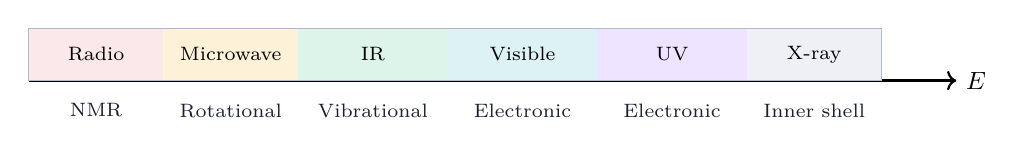
\begin{tikzpicture}[scale=0.95]
  % Energy axis
  \draw[->, thick] (0,0) -- (12.4,0) node[right, font=\small] {$E$};
  % Region bands
  \fill[hdrred]    (0.0,0) rectangle (1.8,0.7);
  \fill[hdramber]  (1.8,0) rectangle (3.6,0.7);
  \fill[hdrgreen]  (3.6,0) rectangle (5.6,0.7);
  \fill[hdrteal]   (5.6,0) rectangle (7.6,0.7);
  \fill[hdrpurple] (7.6,0) rectangle (9.6,0.7);
  \fill[hdrgray]   (9.6,0) rectangle (11.4,0.7);
  \draw[mgframe] (0,0) rectangle (11.4,0.7);
  % Region labels
  \node[font=\scriptsize] at (0.9,0.35)  {Radio};
  \node[font=\scriptsize] at (2.7,0.35)  {Microwave};
  \node[font=\scriptsize] at (4.6,0.35)  {IR};
  \node[font=\scriptsize] at (6.6,0.35)  {Visible};
  \node[font=\scriptsize] at (8.6,0.35)  {UV};
  \node[font=\scriptsize] at (10.5,0.35) {X-ray};
  % Transition labels under
  \node[font=\scriptsize, color=mydark] at (0.9,-0.40)  {NMR};
  \node[font=\scriptsize, color=mydark] at (2.7,-0.40)  {Rotational};
  \node[font=\scriptsize, color=mydark] at (4.6,-0.40)  {Vibrational};
  \node[font=\scriptsize, color=mydark] at (6.6,-0.40)  {Electronic};
  \node[font=\scriptsize, color=mydark] at (8.6,-0.40)  {Electronic};
  \node[font=\scriptsize, color=mydark] at (10.5,-0.40) {Inner shell};
\end{tikzpicture}
\end{tcolorbox}

\textbf{Region--energy mapping:}\par\noindent
\begin{tabularx}{\linewidth}{|B{2.6cm}|Y|Y|Y|}
\hline
\textbf{Region} & \textbf{Wavelength} & \textbf{Energy / quantum} & \textbf{Type of transition} \\
\hline
Radio  & $1\ \mathrm{m}$--$10\ \mathrm{km}$ & very low ($\mu\mathrm{eV}$) & Nuclear spin flip (NMR) \\
\hline
Microwave & $1\ \mathrm{mm}$--$1\ \mathrm{m}$ & $10^{-5}$--$10^{-3}\ \mathrm{eV}$ & Rotational (also ESR) \\
\hline
Infrared (IR) & $700\ \mathrm{nm}$--$1\ \mathrm{mm}$ & $10^{-3}$--$1\ \mathrm{eV}$ & Vibrational \\
\hline
Visible & $400$--$700\ \mathrm{nm}$ & $1.7$--$3.1\ \mathrm{eV}$ & Outer electronic \\
\hline
Ultraviolet (UV) & $10$--$400\ \mathrm{nm}$ & $3.1$--$124\ \mathrm{eV}$ & Outer electronic \\
\hline
X-ray & $0.01$--$10\ \mathrm{nm}$ & $0.1$--$100\ \mathrm{keV}$ & Inner-shell, diffraction \\
\hline
$\gamma$-ray & $<0.01\ \mathrm{nm}$ & $>100\ \mathrm{keV}$ & Nuclear (Mossbauer) \\
\hline
\end{tabularx}

\subsection{Absorption, Emission and Scattering}
Three primary photon-matter events form the basis of every spectroscopic experiment.

\begin{tcolorbox}[tikzbox, title={Three Photon--Matter Processes}]
\centering
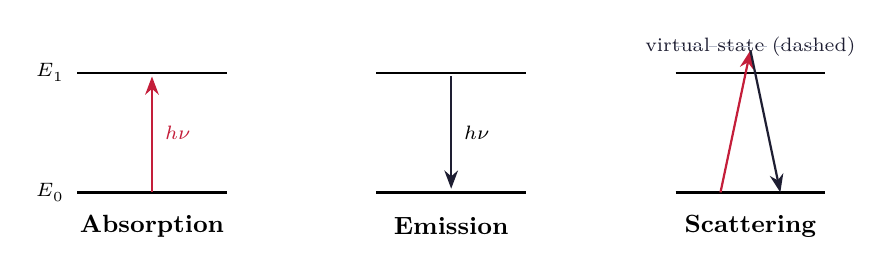
\begin{tikzpicture}[scale=0.95]
  % Absorption
  \draw[thick] (0,0) -- (2.0,0); \node[font=\scriptsize, anchor=east] at (-0.05,0) {$E_0$};
  \draw[thick] (0,1.6) -- (2.0,1.6); \node[font=\scriptsize, anchor=east] at (-0.05,1.6) {$E_1$};
  \draw[redarrow] (1.0,0) -- (1.0,1.55);
  \node[font=\scriptsize, color=myred, anchor=west] at (1.05,0.8) {$h\nu$};
  \node[font=\small\bfseries] at (1.0,-0.45) {Absorption};

  % Emission
  \draw[thick] (4.0,0) -- (6.0,0);
  \draw[thick] (4.0,1.6) -- (6.0,1.6);
  \draw[arrow] (5.0,1.55) -- (5.0,0.05);
  \node[font=\scriptsize, anchor=west] at (5.05,0.8) {$h\nu$};
  \node[font=\small\bfseries] at (5.0,-0.45) {Emission};

  % Scattering
  \draw[thick] (8.0,0) -- (10.0,0);
  \draw[thick] (8.0,1.6) -- (10.0,1.6);
  \node[font=\scriptsize, color=mydark] at (9.0,1.95) {virtual state (dashed)};
  \draw[dashed, mgframe] (8.0,1.95) -- (10.0,1.95);
  \draw[redarrow] (8.6,0) -- (9.0,1.9);
  \draw[arrow] (9.0,1.9) -- (9.4,0);
  \node[font=\small\bfseries] at (9.0,-0.45) {Scattering};
\end{tikzpicture}
\end{tcolorbox}

\textbf{Quick comparison:}\par\noindent
\begin{tabularx}{\linewidth}{|B{2.6cm}|Y|Y|Y|}
\hline
\textbf{Process} & \textbf{What happens} & \textbf{Detected as} & \textbf{Examples} \\
\hline
Absorption & Photon raises molecule from low to high state & Loss of intensity at $\nu$ & UV-Vis, IR \\
\hline
Emission & Excited molecule drops back, releasing photon & Light at characteristic $\nu$ & Fluorescence, AES \\
\hline
Scattering & Photon redirected (with or without energy change) & Light at angle from beam & Raman, X-ray scattering \\
\hline
\end{tabularx}

\subsection{Resonance Condition and the Bohr Frequency Rule}
A photon is absorbed only when its energy matches the gap between two molecular energy levels. This is the \emph{resonance condition}.

\begin{tcolorbox}[formulabox, title={Bohr Frequency Condition}]
\[
\Delta E = E_2 - E_1 = h\nu = \frac{hc}{\lambda} = hc\bar{\nu}
\]
Only photons with this exact $\nu$ are absorbed. Off-resonance photons pass through unchanged. This is why spectra show \emph{discrete lines or bands} instead of a continuum.
\end{tcolorbox}

\subsection{Selection Rules: Allowed and Forbidden Transitions}
Even when the resonance condition is satisfied, a transition occurs only if the corresponding selection rule is obeyed. Selection rules come from the requirement that the transition dipole moment integral be non-zero.

\begin{tcolorbox}[formulabox, title={Transition Probability and Dipole Moment}]
\[
P_{1\to2} \propto |\,\mu_{12}\,|^{2}, \qquad
\mu_{12}=\int \psi_2^{*}\,\hat{\mu}\,\psi_1\,d\tau
\]
\textbf{Allowed} transition: $\mu_{12}\neq 0$ — strong band, high intensity.\\
\textbf{Forbidden} transition: $\mu_{12}=0$ in the simple model — band absent or very weak.
\end{tcolorbox}

\textbf{Two general selection rules:}
\begin{enumerate}[leftmargin=*, itemsep=2pt, topsep=2pt]
  \item \textbf{Gross selection rule:} The molecule must possess a property (e.g.\ permanent or oscillating dipole) capable of interacting with the radiation.
  \item \textbf{Specific selection rule:} The change in quantum numbers must obey definite values, e.g.\ $\Delta v = \pm 1$, $\Delta J = \pm 1$, $\Delta l = \pm 1$.
\end{enumerate}

\textbf{Selection rules across spectroscopies:}\par\noindent
\begin{tabularx}{\linewidth}{|B{2.8cm}|Y|Y|}
\hline
\textbf{Spectroscopy} & \textbf{Gross rule (must have)} & \textbf{Specific rule} \\
\hline
Rotational (microwave) & Permanent electric dipole moment & $\Delta J=\pm 1$ \\
\hline
Vibrational (IR) & Vibration must change dipole moment & $\Delta v=\pm 1$ (harmonic); $\pm 1, \pm 2,\ldots$ (anharmonic) \\
\hline
Raman & Vibration must change polarisability & $\Delta v=\pm 1$; $\Delta J=0,\pm 2$ \\
\hline
Electronic (UV-Vis) & Allowed orbital symmetry transition & $\Delta S=0$ (spin); $\Delta l=\pm 1$ (Laporte) \\
\hline
NMR & Magnetic spin $I\neq 0$ in field $B_0$ & $\Delta m_I=\pm 1$ \\
\hline
ESR & Unpaired electron $S\neq 0$ & $\Delta m_S=\pm 1$ \\
\hline
\end{tabularx}

\begin{tcolorbox}[examplebox, title={Solved Example: Why \texorpdfstring{$\mathrm{N_2}$}{N2} Shows No IR but Shows Raman}]
\textbf{Problem:} Predict whether $\mathrm{N_2}$ molecule shows IR absorption or Raman scattering.

\textbf{Solution:} For IR, the vibration must change the molecular dipole moment.\\
$\mathrm{N_2}$ is homonuclear, so its dipole moment is zero throughout the stretching vibration. \\$\Rightarrow$ IR-\textbf{inactive}.\\
For Raman, the vibration must change the polarisability of the electron cloud. The $\mathrm{N{\equiv}N}$ stretch does change polarisability. \\$\Rightarrow$ Raman-\textbf{active}.
\end{tcolorbox}

\begin{tcolorbox}[masonbox, title={Mutual Exclusion Principle}]
For molecules with a centre of symmetry (e.g.\ $\mathrm{CO_2}$, $\mathrm{N_2}$), a vibration that is IR-active is Raman-inactive, and vice-versa. This rule is a powerful structural fingerprint and a common viva question.
\end{tcolorbox}

\subsection{Population of Energy Levels: Boltzmann Distribution}
The intensity of an absorption line depends on how many molecules occupy the lower level at thermal equilibrium. The Boltzmann distribution governs this population.

\begin{tcolorbox}[formulabox, title={Boltzmann Population Ratio}]
\[
\frac{N_2}{N_1}=\frac{g_2}{g_1}\,\exp\!\left(-\frac{\Delta E}{k_B T}\right)
\]
where $g_1, g_2$ are degeneracies, $k_B=1.381\times10^{-23}\ \mathrm{J\,K^{-1}}$ and $T$ is temperature in K.
\end{tcolorbox}

\textbf{Implication:} Microwave (rotational) transitions involve very small $\Delta E$, so excited rotational levels are well populated even at room temperature. NMR transitions involve $\Delta E\ll k_BT$, so the population difference is tiny — that is why NMR is intrinsically a low-sensitivity technique.

\subsection{Resolution and Linewidth: The Heisenberg Limit}
Spectral lines are not infinitely sharp. They have natural widths set by the lifetime of the excited state through Heisenberg's uncertainty principle.

\begin{tcolorbox}[formulabox, title={Natural Linewidth}]
\[
\Delta E\cdot\Delta t \gtrsim \frac{\hbar}{2}, \qquad \Delta\nu \approx \frac{1}{2\pi\tau}
\]
A short excited-state lifetime $\tau$ produces a broad line; a long lifetime gives a sharp line.
\end{tcolorbox}

\textbf{Other broadening sources:} Doppler broadening (gas phase), collisional broadening (high pressure), and instrumental broadening.

\subsection{Transmittance vs Absorbance}
Two scales describe how much light a sample lets through. Confusing them is the most common 2-mark error.

\begin{tcolorbox}[formulabox, title={Transmittance and Absorbance}]
\[
T=\frac{I}{I_0}, \qquad \%T=100\,T, \qquad A=-\log_{10}T=\log_{10}\!\frac{I_0}{I}
\]
$T$ is linear in light intensity but \emph{non-linear} in concentration. $A$ is linear in concentration through Beer--Lambert. Always plot $A$, never $T$, against concentration for calibration.
\end{tcolorbox}

\subsection{Einstein A and B Coefficients}
Einstein analysed the equilibrium between matter and radiation by introducing three rate constants for the photon--matter exchange.

\begin{tcolorbox}[formulabox, title={Einstein Coefficients}]
\textbf{Stimulated absorption rate:} $\;R_{12}=B_{12}\,N_1\,\rho(\nu)$\\
\textbf{Stimulated emission rate:} $\;R_{21}^{\mathrm{stim}}=B_{21}\,N_2\,\rho(\nu)$\\
\textbf{Spontaneous emission rate:} $\;R_{21}^{\mathrm{spon}}=A_{21}\,N_2$\\
At thermal equilibrium,
\[
\frac{A_{21}}{B_{21}}=\frac{8\pi h\nu^{3}}{c^{3}}, \qquad B_{12}\,g_1=B_{21}\,g_2
\]
$\rho(\nu)$ is the radiation density at frequency $\nu$.
\end{tcolorbox}

\textbf{Why this matters:} The $\nu^{3}$ scaling shows that spontaneous emission dominates at high frequencies (visible/UV $\Rightarrow$ fluorescence) while stimulated processes dominate at low frequencies (microwave/RF $\Rightarrow$ NMR sensitivity problem). This is the theoretical basis for both lasers (population inversion makes $B_{21}$ exceed $B_{12}$ rates) and the weak NMR signal at room temperature.

\subsection{Franck--Condon Principle}
Electronic transitions are vertical on a potential-energy diagram because nuclei are too heavy to move during the $10^{-15}\ \mathrm{s}$ duration of an electronic absorption.

\begin{tcolorbox}[defbox]
\textbf{Franck--Condon principle:} An electronic transition is most probable when the vibrational wave functions of the two states have the largest overlap. Because the transition is vertical, the molecule lands in a vibrationally excited level of the upper electronic state.
\end{tcolorbox}

\begin{tcolorbox}[tikzbox, title={Franck--Condon Vertical Transitions and Vibrational Progression}]
\centering
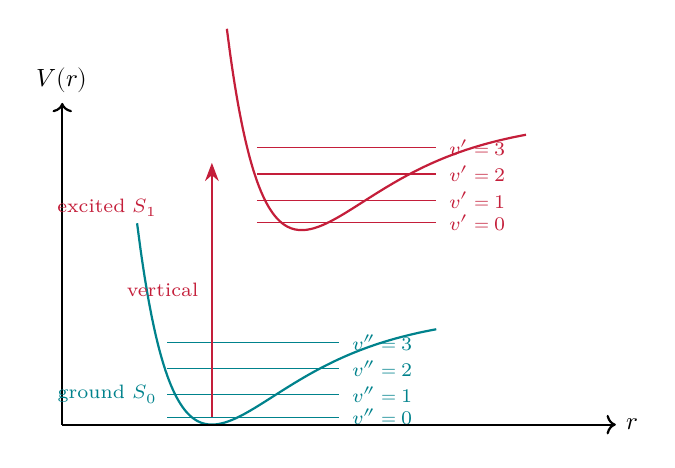
\begin{tikzpicture}[scale=0.95]
  % Lower state Morse
  \draw[myteal, thick, domain=-1.0:3.0, samples=80, smooth, variable=\x] plot ({\x+2.0},{1.5*(1-exp(-0.85*\x))^2});
  % Upper state Morse (shifted right and up)
  \draw[myred, thick, domain=-1.0:3.0, samples=80, smooth, variable=\x] plot ({\x+3.2},{2.6+1.5*(1-exp(-0.85*\x))^2});
  % vibrational levels
  \foreach \v/\y in {0/0.10, 1/0.40, 2/0.75, 3/1.10} {
     \draw[thin, myteal] (1.4,\y) -- (3.7,\y); \node[font=\scriptsize, color=myteal, anchor=west] at (3.75,\y) {$v''=\v$};
  }
  \foreach \v/\y in {0/2.70, 1/3.00, 2/3.35, 3/3.70} {
     \draw[thin, myred] (2.6,\y) -- (5.0,\y);  \node[font=\scriptsize, color=myred, anchor=west] at (5.05,\y) {$v'=\v$};
  }
  % Vertical transition
  \draw[redarrow] (2.0,0.10) -- (2.0,3.50);
  \node[font=\scriptsize, color=myred, anchor=east] at (1.95,1.8) {vertical};
  % axes
  \draw[->, thick] (0,0) -- (7.4,0) node[right, font=\small] {$r$};
  \draw[->, thick] (0,0) -- (0,4.3) node[above, font=\small] {$V(r)$};
  \node[font=\scriptsize, color=myteal] at (0.6,0.4) {ground $S_0$};
  \node[font=\scriptsize, color=myred]  at (0.6,2.9) {excited $S_1$};
\end{tikzpicture}
\end{tcolorbox}

\textbf{Consequences of the Franck--Condon principle:}
\begin{itemize}[leftmargin=*, itemsep=2pt, topsep=2pt]
  \item Absorption spectra of polyatomic molecules show \emph{vibrational fine structure} (a band, not a line).
  \item The most intense vibronic line corresponds to the maximum-overlap (largest Franck--Condon factor) vibrational pair.
  \item After absorption, vibrational relaxation back to $v'=0$ explains the Stokes shift seen in fluorescence.
  \item Combined with Kasha's rule (next sections), it explains why fluorescence emission spectra are wavelength-independent of the excitation $\lambda$.
\end{itemize}

\begin{tcolorbox}[exambox, title={Exam Points (Section 1)}]
\begin{itemize}[leftmargin=*, itemsep=2pt, topsep=2pt]
  \item Always link region of EM spectrum to type of energy: radio--NMR, microwave--rotation, IR--vibration, UV-Vis--electronic.
  \item Use $E=h\nu=hc/\lambda=hc\bar{\nu}$ — examiners love unit conversion problems.
  \item Quote both the gross and specific selection rules; missing the gross rule is the most common cut.
  \item Mutual exclusion principle is a 2-mark gem; remember $\mathrm{CO_2}$.
  \item For NMR sensitivity question, refer to the Boltzmann ratio.
  \item Franck--Condon principle: ``electronic transitions are vertical, nuclei don't move''.
  \item Einstein relation $A_{21}/B_{21}=8\pi h\nu^{3}/c^{3}$ — explains why low-frequency NMR is intrinsically weak.
\end{itemize}
\end{tcolorbox}

% ===============================================================================
\section{Electronic (UV-Visible) Spectroscopy}
% ===============================================================================

\begin{tcolorbox}[defbox]
\textbf{Electronic spectroscopy} (UV-Vis) measures absorption of ultraviolet ($200$--$400\ \mathrm{nm}$) and visible ($400$--$800\ \mathrm{nm}$) light by molecules. The energy is sufficient to promote a valence electron from a filled orbital to an empty higher-energy orbital. The resulting spectrum gives information about chromophores, conjugation, and concentration.
\end{tcolorbox}

\subsection{Types of Electronic Transitions}
The valence electrons of organic molecules occupy four kinds of orbitals: bonding $\sigma$ and $\pi$, non-bonding $n$, and antibonding $\sigma^{*}$ and $\pi^{*}$. The four common electronic transitions, in increasing wavelength (decreasing energy), are listed below.

\begin{tcolorbox}[tikzbox, title={Energy-Level Order of Molecular Orbitals and Possible Transitions}]
\centering
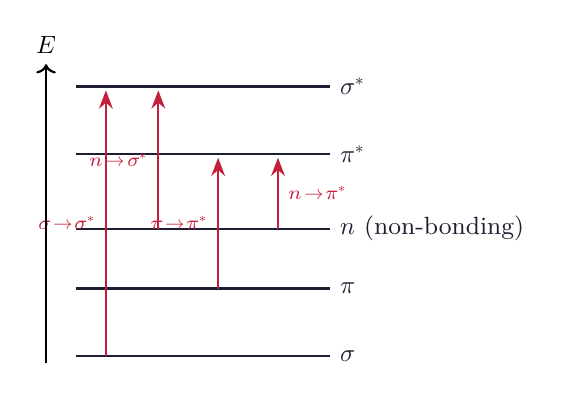
\begin{tikzpicture}[scale=0.95]
  % Levels
  \draw[thick, mydark] (0,0)   -- (3.4,0)   node[right, font=\small] {$\sigma$};
  \draw[thick, mydark] (0,0.9) -- (3.4,0.9) node[right, font=\small] {$\pi$};
  \draw[thick, mydark] (0,1.7) -- (3.4,1.7) node[right, font=\small] {$n$ (non-bonding)};
  \draw[thick, mydark] (0,2.7) -- (3.4,2.7) node[right, font=\small] {$\pi^{*}$};
  \draw[thick, mydark] (0,3.6) -- (3.4,3.6) node[right, font=\small] {$\sigma^{*}$};

  % Transitions (arrows)
  \draw[redarrow] (0.4,0)   -- (0.4,3.55) node[midway, left, font=\scriptsize, color=myred] {$\sigma\!\to\!\sigma^{*}$};
  \draw[redarrow] (1.1,1.7) -- (1.1,3.55) node[midway, left, font=\scriptsize, color=myred] {$n\!\to\!\sigma^{*}$};
  \draw[redarrow] (1.9,0.9) -- (1.9,2.65) node[midway, left, font=\scriptsize, color=myred] {$\pi\!\to\!\pi^{*}$};
  \draw[redarrow] (2.7,1.7) -- (2.7,2.65) node[midway, right, font=\scriptsize, color=myred] {$n\!\to\!\pi^{*}$};

  % Energy axis
  \draw[->, thick] (-0.4,-0.1) -- (-0.4,3.9) node[above, font=\small] {$E$};
\end{tikzpicture}
\end{tcolorbox}

\textbf{Comparison of the four transitions:}\par\noindent
\begin{tabularx}{\linewidth}{|B{2.4cm}|Y|Y|Y|}
\hline
\textbf{Transition} & \textbf{Compounds showing it} & \textbf{$\lambda_{\max}$ region} & \textbf{Intensity ($\varepsilon$)} \\
\hline
$\sigma\!\to\!\sigma^{*}$ & Saturated alkanes (CH$_4$, ethane) & $<150\ \mathrm{nm}$ (vacuum UV) & High but inaccessible \\
\hline
$n\!\to\!\sigma^{*}$ & H$_2$O, CH$_3$OH, alkyl halides, amines & $150$--$250\ \mathrm{nm}$ & Medium ($10^2$--$10^3$) \\
\hline
$\pi\!\to\!\pi^{*}$ & Alkenes, alkynes, aromatics, carbonyls & $170$--$250\ \mathrm{nm}$ & High ($10^3$--$10^4$) \\
\hline
$n\!\to\!\pi^{*}$ & Aldehydes, ketones, $\mathrm{>C{=}O}$, $\mathrm{>C{=}N}$ & $270$--$300\ \mathrm{nm}$ & Low ($10$--$10^2$) \\
\hline
\end{tabularx}

\subsection{Beer--Lambert Law: The Quantitative Backbone}
UV-Vis is a quantitative tool because the absorbance is linearly related to concentration through the Beer--Lambert law.

\begin{tcolorbox}[formulabox, title={Beer--Lambert Law}]
\[
A=\log_{10}\!\frac{I_0}{I}=\varepsilon\,c\,l
\]
\textbf{Symbols:} $A$ = absorbance (dimensionless); $I_0$ = incident intensity; $I$ = transmitted intensity; $\varepsilon$ = molar absorptivity ($\mathrm{L\,mol^{-1}\,cm^{-1}}$); $c$ = concentration ($\mathrm{mol\,L^{-1}}$); $l$ = path length (cm).\\
Also useful:
\[
T=\frac{I}{I_0},\qquad A=-\log_{10}T=2-\log_{10}(\%T)
\]
\end{tcolorbox}

\textbf{Limitations of Beer--Lambert law:}\par\noindent
\begin{tabularx}{\linewidth}{|B{3.4cm}|Y|}
\hline
\textbf{Cause of deviation} & \textbf{Reason} \\
\hline
High concentration ($>10^{-2}\ \mathrm{M}$) & Solute molecules interact, $\varepsilon$ is no longer constant \\
\hline
Polychromatic light & Different wavelengths have different $\varepsilon$, average becomes non-linear \\
\hline
Stray radiation & Light reaching detector by leakage flattens absorbance at high $A$ \\
\hline
Chemical equilibria & Dimerisation, ionisation, fluorescence change effective absorbing species \\
\hline
\end{tabularx}

\begin{tcolorbox}[examplebox, title={Solved Example: Absorbance to Concentration}]
\textbf{Problem:} A solution of an organic dye gives $A=0.92$ in a $1.0\ \mathrm{cm}$ cell at $510\ \mathrm{nm}$, where $\varepsilon=2300\ \mathrm{L\,mol^{-1}\,cm^{-1}}$. Find the concentration.

\textbf{Solution:} From $A=\varepsilon c l$,
\[
c=\frac{A}{\varepsilon l}=\frac{0.92}{2300\times 1.0}=4.0\times 10^{-4}\ \mathrm{mol\,L^{-1}}
\]
\textbf{Exam tip:} Always state whether you used $\log_{10}$ or $\ln$. The IUPAC form uses $\log_{10}$.
\end{tcolorbox}

\subsection{Chromophores and Auxochromes}
Functional groups that determine where a molecule absorbs are called chromophores, while certain saturated groups that shift the band of a chromophore are called auxochromes.

\begin{tcolorbox}[defbox]
\textbf{Chromophore:} Unsaturated functional group responsible for absorption (e.g.\ $\mathrm{C{=}C}$, $\mathrm{C{=}O}$, $\mathrm{N{=}N}$, $\mathrm{NO_2}$).\\
\textbf{Auxochrome:} Saturated group with non-bonding electrons (e.g.\ $\mathrm{-OH}$, $\mathrm{-NH_2}$, $\mathrm{-OR}$, $\mathrm{-X}$) that, when attached to a chromophore, shifts $\lambda_{\max}$ to longer wavelength and increases intensity.
\end{tcolorbox}

\textbf{Standard wavelength-shift terminology:}\par\noindent
\begin{tabularx}{\linewidth}{|B{2.6cm}|Y|Y|}
\hline
\textbf{Term} & \textbf{Effect on $\lambda_{\max}$} & \textbf{Cause} \\
\hline
Bathochromic (red) shift & $\lambda_{\max}$ \emph{increases} & Conjugation, auxochrome, polar solvent (for $\pi\!\to\!\pi^{*}$) \\
\hline
Hypsochromic (blue) shift & $\lambda_{\max}$ \emph{decreases} & Removal of conjugation, polar solvent (for $n\!\to\!\pi^{*}$) \\
\hline
Hyperchromic effect & $\varepsilon$ \emph{increases} & Increased symmetry/conjugation \\
\hline
Hypochromic effect & $\varepsilon$ \emph{decreases} & Distortion of chromophore \\
\hline
\end{tabularx}

\subsection{Effect of Conjugation}
Each additional conjugated $\mathrm{C{=}C}$ raises the highest occupied $\pi$ MO and lowers the lowest empty $\pi^{*}$ MO. The HOMO--LUMO gap shrinks, so $\lambda_{\max}$ moves to longer wavelength.

\begin{tabularx}{\linewidth}{|B{3.0cm}|Y|Y|}
\hline
\textbf{Compound} & \textbf{Conjugated double bonds} & \textbf{$\lambda_{\max}$ (nm)} \\
\hline
Ethylene & 1 & 165 \\
\hline
1,3-Butadiene & 2 & 217 \\
\hline
1,3,5-Hexatriene & 3 & 258 \\
\hline
$\beta$-Carotene & 11 & 470 (orange colour) \\
\hline
\end{tabularx}

\subsection{Solvent Effects on Electronic Spectra}
The solvent stabilises the ground and excited states differently, so the absorption band shifts.

\begin{tabularx}{\linewidth}{|B{2.4cm}|Y|Y|}
\hline
\textbf{Transition} & \textbf{Polar protic solvent effect} & \textbf{Reason} \\
\hline
$\pi\!\to\!\pi^{*}$ & Bathochromic (red shift) & Excited state ($\pi^{*}$) more polar, better stabilised \\
\hline
$n\!\to\!\pi^{*}$ & Hypsochromic (blue shift) & Hydrogen bonds with lone pair lower the ground state more \\
\hline
\end{tabularx}

\subsection{Block Diagram of a UV-Visible Spectrophotometer}
A double-beam spectrophotometer compares the sample beam with a reference beam in real time, eliminating fluctuations of the lamp.

\begin{tcolorbox}[tikzbox, title={Double-Beam UV-Vis Spectrophotometer}]
\centering
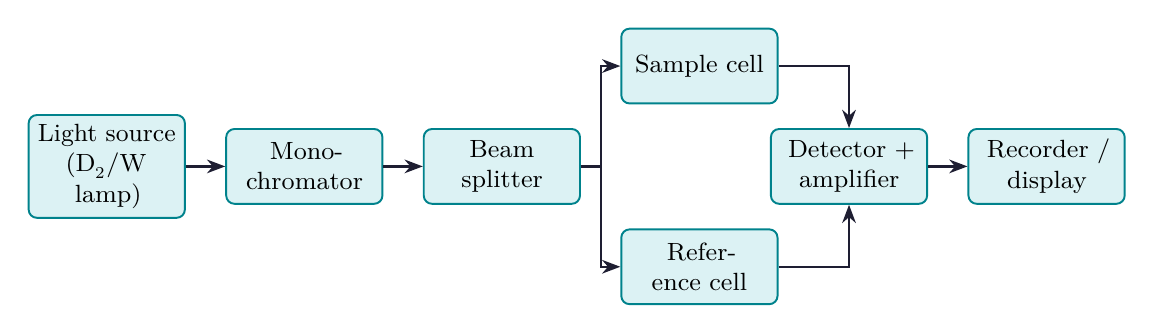
\begin{tikzpicture}[node distance=0.3cm and 0.45cm,
  sblock/.style={rectangle, draw=myteal, fill=hdrteal, text width=1.75cm,
    align=center, minimum height=0.95cm, font=\small,
    rounded corners=3pt, line width=0.7pt}]
  \node[sblock] (n1) {Light source\\(D$_2$/W lamp)};
  \node[sblock, right=0.5cm of n1] (n2) {Mono-chromator};
  \node[sblock, right=0.5cm of n2] (n3) {Beam splitter};
  \node[sblock, above right=0.3cm and 0.5cm of n3] (n4) {Sample cell};
  \node[sblock, below right=0.3cm and 0.5cm of n3] (n5) {Reference cell};
  \node[sblock, right=2.4cm of n3] (n6) {Detector + amplifier};
  \node[sblock, right=0.5cm of n6] (n7) {Recorder /\\display};

  \draw[arrow] (n1) -- (n2);
  \draw[arrow] (n2) -- (n3);
  \draw[arrow] (n3.east) -- ++(0.25,0) |- (n4.west);
  \draw[arrow] (n3.east) -- ++(0.25,0) |- (n5.west);
  \draw[arrow] (n4.east) -| (n6.north);
  \draw[arrow] (n5.east) -| (n6.south);
  \draw[arrow] (n6) -- (n7);
\end{tikzpicture}
\end{tcolorbox}

\textbf{Common light sources and their range:}
\begin{itemize}[leftmargin=*, itemsep=1pt, topsep=2pt]
  \item Deuterium ($\mathrm{D_2}$) lamp — UV region, $190$--$400\ \mathrm{nm}$.
  \item Tungsten--halogen lamp — visible region, $350$--$2500\ \mathrm{nm}$.
  \item Xenon flash lamp — both UV and visible.
\end{itemize}

\subsection{Applications of UV-Visible Spectroscopy}
\begin{itemize}[leftmargin=*, itemsep=2pt, topsep=2pt]
  \item Quantitative estimation of metal ions (Fe$^{3+}$ as thiocyanate, etc.).
  \item Determination of molar absorptivity and concentration in pharmaceuticals.
  \item Detection of conjugated systems and aromatic rings.
  \item Reaction kinetics: change in $A$ with time gives the rate.
  \item Identification of dyes and impurity profiling.
\end{itemize}

\subsection{Woodward--Fieser Rules}
For dienes and $\alpha,\beta$-unsaturated carbonyls, $\lambda_{\max}$ can be predicted to within $\pm 5\ \mathrm{nm}$ by adding empirical increments to a base value. This is a MAKAUT favourite for 5- and 10-mark questions.

\begin{tcolorbox}[formulabox, title={Woodward--Fieser Rule for Dienes}]
\[
\lambda_{\max} = \lambda_{\mathrm{base}} + \sum (\text{increments})
\]
Base values (in nm):\\[2pt]
Acyclic / heteroannular diene: $\bf 215$ \quad Homoannular diene: $\bf 253$\\[6pt]
Common increments:
\begin{itemize}[leftmargin=*, itemsep=1pt, topsep=2pt]
  \item Each extra conjugated $\mathrm{C{=}C}$: $+30$
  \item Alkyl group / ring residue: $+5$
  \item Exocyclic double bond: $+5$
  \item $-\mathrm{OR}$: $+6$, $-\mathrm{OAc}$: $0$, $-\mathrm{Cl}/-\mathrm{Br}$: $+5$, $-\mathrm{NR_2}$: $+60$
\end{itemize}
\end{tcolorbox}

\begin{tcolorbox}[examplebox, title={Solved Example: Predicting \texorpdfstring{$\lambda_{\max}$}{lambda max} of 2,4-Dimethyl-1,3-pentadiene}]
\textbf{Structure:} acyclic diene with two methyl substituents and one ring residue.

\textbf{Calculation:}
\begin{itemize}[leftmargin=*, itemsep=1pt, topsep=2pt]
  \item Base value (acyclic diene) \dotfill $215$
  \item Three alkyl groups $\times +5$ \dotfill $+15$
\end{itemize}
\[
\lambda_{\max}^{\text{pred}} = 215 + 15 = 230\ \mathrm{nm}
\]
\textbf{Reported:} $\lambda_{\max}=232\ \mathrm{nm}$ — within the $\pm 5\ \mathrm{nm}$ rule.
\end{tcolorbox}

\textbf{Woodward--Fieser rule for enones:} The rule extends to $\alpha,\beta$-unsaturated ketones with base value $215\ \mathrm{nm}$ (acyclic / six-ring) and base value $202\ \mathrm{nm}$ (five-ring). Each $\alpha$-substituent adds $10\ \mathrm{nm}$, $\beta$-substituent adds $12\ \mathrm{nm}$, and so on. Beyond the engineering syllabus the principle is the same — pile up empirical increments on a base.

\subsection{Isosbestic Point}
When two species $A$ and $B$ inter-convert (e.g.\ acid--base equilibrium or a kinetic transformation), their UV-Vis spectra cross at one or more wavelengths where the absorbance does \emph{not} change with composition.

\begin{tcolorbox}[defbox]
\textbf{Isosbestic point:} A wavelength at which two absorbing species have the same molar absorptivity. The presence of a sharp isosbestic point in a series of recorded spectra is direct evidence of a clean two-component equilibrium without any third absorbing intermediate.
\end{tcolorbox}

\textbf{Why exam-relevant:} In titrations, kinetic studies, and pH-dependent measurements the isosbestic point lets you measure total concentration independent of the equilibrium position.

\subsection{Single-Beam vs Double-Beam Instruments}
\begin{tabularx}{\linewidth}{|B{2.6cm}|Y|Y|}
\hline
\textbf{Feature} & \textbf{Single-beam} & \textbf{Double-beam} \\
\hline
Light path & One path: source $\to$ sample $\to$ detector & Two paths simultaneously: sample and reference \\
\hline
Reference correction & Manual (run blank, then sample) & Automatic, real-time \\
\hline
Lamp drift & Affects reading & Cancelled out \\
\hline
Cost & Cheaper, simpler & More expensive but more accurate \\
\hline
Use case & Routine fixed-$\lambda$ measurements & Spectral scanning, kinetics \\
\hline
\end{tabularx}

\subsection{Sample Cell (Cuvette) Materials}
Choosing the wrong cuvette is the most common practical mistake — quartz absorbs nothing in UV, glass cuts off below $340\ \mathrm{nm}$.

\begin{tabularx}{\linewidth}{|B{2.6cm}|Y|Y|}
\hline
\textbf{Material} & \textbf{Useful range} & \textbf{Notes} \\
\hline
Quartz / fused silica & $190$--$2500\ \mathrm{nm}$ & Mandatory for UV; expensive \\
\hline
Borosilicate glass & $340$--$2500\ \mathrm{nm}$ & Visible/NIR only \\
\hline
Polystyrene (disposable) & $340$--$800\ \mathrm{nm}$ & Single-use, cheap, visible only \\
\hline
$\mathrm{CaF_2}$ / $\mathrm{BaF_2}$ & $150\ \mathrm{nm}$--mid-IR & Vacuum-UV and IR work \\
\hline
\end{tabularx}

\begin{tcolorbox}[exambox, title={Exam Points (Section 2)}]
\begin{itemize}[leftmargin=*, itemsep=2pt, topsep=2pt]
  \item State all four transitions with energy order: $n\!\to\!\pi^{*}<\pi\!\to\!\pi^{*}<n\!\to\!\sigma^{*}<\sigma\!\to\!\sigma^{*}$.
  \item For Beer--Lambert numericals, watch units of $c$ and $l$.
  \item Always link conjugation with bathochromic shift ($\beta$-carotene, lycopene).
  \item Mention deuterium lamp for UV and tungsten lamp for visible.
  \item Use the Woodward--Fieser increment formula for enone / diene predictions.
  \item Quartz cuvette below $340\ \mathrm{nm}$, glass above $340\ \mathrm{nm}$.
  \item Sharp isosbestic point $=$ clean two-component equilibrium.
\end{itemize}
\end{tcolorbox}

% ===============================================================================
\section{Fluorescence and Its Applications in Medicine}
% ===============================================================================

\begin{tcolorbox}[defbox]
\textbf{Fluorescence} is the spontaneous emission of light by a molecule that has been excited to a higher singlet electronic state, when it returns to its ground state \emph{without changing spin multiplicity}. The emission lifetime is short ($10^{-9}$--$10^{-7}\ \mathrm{s}$), and the emission stops as soon as the exciting source is turned off.
\end{tcolorbox}

\subsection{Singlet, Triplet and the Jablonski Diagram}
A molecule can have its electron pair with antiparallel spins (singlet, $S$) or parallel spins (triplet, $T$). All photophysical processes can be summarised in a Jablonski diagram.

\begin{tcolorbox}[tikzbox, title={Jablonski Energy-Level Diagram}]
\centering
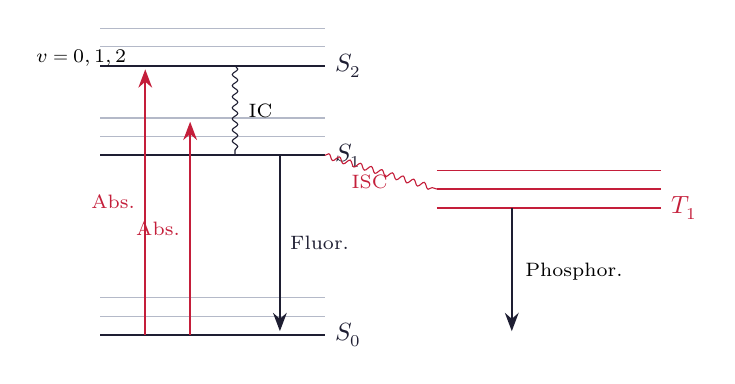
\begin{tikzpicture}[scale=0.95]
  % Singlet manifolds
  \draw[thick, mydark] (0,0) -- (3.0,0)   node[right, font=\small] {$S_0$};
  \draw[thick, mydark] (0,2.4) -- (3.0,2.4) node[right, font=\small] {$S_1$};
  \draw[thick, mydark] (0,3.6) -- (3.0,3.6) node[right, font=\small] {$S_2$};
  % Vibrational sub-levels
  \foreach \y in {0.25, 0.5}  \draw[thin, mgframe] (0,\y) -- (3.0,\y);
  \foreach \y in {2.65, 2.9} \draw[thin, mgframe] (0,\y) -- (3.0,\y);
  \foreach \y in {3.85, 4.1} \draw[thin, mgframe] (0,\y) -- (3.0,\y);
  % Triplet
  \draw[thick, myred] (4.5,1.7) -- (7.5,1.7) node[right, font=\small, color=myred] {$T_1$};
  \foreach \y in {1.95, 2.2} \draw[thin, myred] (4.5,\y) -- (7.5,\y);

  % Absorption arrows
  \draw[redarrow] (0.6,0)   -- (0.6,3.55) node[midway, left, font=\scriptsize, color=myred] {Abs.};
  \draw[redarrow] (1.2,0)   -- (1.2,2.85) node[midway, left, font=\scriptsize, color=myred] {Abs.};

  % IC (internal conversion) wavy down
  \draw[decorate, decoration={snake, amplitude=1pt, segment length=4pt}, color=mydark]
       (1.8,3.6) -- (1.8,2.4);
  \node[font=\scriptsize, anchor=west] at (1.85,3.0) {IC};

  % Fluorescence
  \draw[arrow] (2.4,2.4) -- (2.4,0.05) node[midway, right, font=\scriptsize] {Fluor.};

  % Inter-system crossing
  \draw[decorate, decoration={snake, amplitude=1pt, segment length=4pt}, color=myred]
       (3.0,2.4) -- (4.5,1.95);
  \node[font=\scriptsize, color=myred] at (3.6,2.05) {ISC};

  % Phosphorescence
  \draw[arrow] (5.5,1.7) -- (5.5,0.05);
  \node[font=\scriptsize, anchor=west] at (5.55,0.85) {Phosphor.};

  % Vibrational relaxation labels
  \node[font=\scriptsize] at (-0.25,3.7) {$v=0,1,2$};
\end{tikzpicture}
\end{tcolorbox}

\textbf{Key processes shown in the Jablonski diagram:}
\begin{itemize}[leftmargin=*, itemsep=2pt, topsep=2pt]
  \item \textbf{Absorption}: $S_0\to S_1$ or $S_0\to S_2$ in $10^{-15}\ \mathrm{s}$.
  \item \textbf{Vibrational relaxation (VR)}: loss of excess vibrational energy in $10^{-12}\ \mathrm{s}$.
  \item \textbf{Internal conversion (IC)}: non-radiative $S_2\to S_1$, same multiplicity.
  \item \textbf{Fluorescence (F)}: radiative $S_1\to S_0$ in $10^{-9}$--$10^{-7}\ \mathrm{s}$.
  \item \textbf{Inter-system crossing (ISC)}: $S_1\to T_1$, spin-forbidden but possible.
  \item \textbf{Phosphorescence (P)}: radiative $T_1\to S_0$ in $10^{-3}$--$10\ \mathrm{s}$.
\end{itemize}

\subsection{Fluorescence vs Phosphorescence}
\begin{tabularx}{\linewidth}{|B{3.0cm}|Y|Y|}
\hline
\textbf{Property} & \textbf{Fluorescence} & \textbf{Phosphorescence} \\
\hline
Initial state & Singlet excited ($S_1$) & Triplet excited ($T_1$) \\
\hline
Spin change & None (allowed) & Yes (formally forbidden) \\
\hline
Lifetime & $10^{-9}$--$10^{-7}\ \mathrm{s}$ & $10^{-3}$--$10\ \mathrm{s}$ \\
\hline
After source off & Stops immediately & Persists (afterglow) \\
\hline
Wavelength & Slightly higher than absorption & Even higher than fluorescence \\
\hline
Common at & Room temperature, fluid solution & Low temperature, rigid medium \\
\hline
\end{tabularx}

\subsection{Stokes Shift and Mirror-Image Rule}
\begin{tcolorbox}[defbox]
\textbf{Stokes shift} is the difference between the absorption maximum and the emission maximum, $\Delta\lambda=\lambda_{\mathrm{em}}-\lambda_{\mathrm{abs}}$. It arises because the molecule loses vibrational energy before emitting.\\
\textbf{Mirror-image rule:} For most rigid fluorophores the emission spectrum is approximately a mirror image of the absorption spectrum on the wavelength axis.
\end{tcolorbox}

\subsection{Quantum Yield and Quenching}
\begin{tcolorbox}[formulabox, title={Quantum Yield of Fluorescence}]
\[
\Phi_F=\frac{\text{number of photons emitted}}{\text{number of photons absorbed}}=\frac{k_F}{k_F+k_{NR}+k_{ISC}+k_Q[Q]}
\]
$k_F$ is the radiative rate; $k_{NR}, k_{ISC}, k_Q$ are non-radiative, inter-system crossing and quenching rates respectively. $0\le \Phi_F\le 1$.
\end{tcolorbox}

\textbf{Stern--Volmer equation for collisional quenching:}
\[
\frac{F_0}{F}=1+K_{SV}[Q]
\]
where $F_0$ is fluorescence intensity without quencher, $F$ is intensity in presence of quencher concentration $[Q]$, and $K_{SV}$ is the Stern--Volmer constant.

\subsection{Factors Influencing Fluorescence Intensity}
\begin{tabularx}{\linewidth}{|B{3.4cm}|Y|}
\hline
\textbf{Factor} & \textbf{Effect} \\
\hline
Rigidity of molecule & Rigid planar systems (fluorescein, rhodamine) fluoresce strongly because non-radiative pathways are suppressed. \\
\hline
Conjugation / aromaticity & Extended $\pi$-system shifts emission to longer $\lambda$ and increases $\Phi_F$. \\
\hline
Substituents & Electron-donating ($-\mathrm{NH_2}, -\mathrm{OH}$) enhance; heavy atoms (Br, I) and $\mathrm{NO_2}$ promote ISC and quench. \\
\hline
Solvent & Polar solvent stabilises the more polar excited state $\Rightarrow$ red-shifted, sometimes weaker emission. \\
\hline
Temperature & Higher $T$ increases collisional non-radiative loss $\Rightarrow$ weaker fluorescence. \\
\hline
Dissolved $\mathrm{O_2}$ & Triplet $\mathrm{O_2}$ quenches both fluorescence and phosphorescence. \\
\hline
pH & Protonation/deprotonation of acidic chromophores changes $\Phi_F$ and $\lambda_{em}$. \\
\hline
\end{tabularx}

\subsection{Spectrofluorimeter (Block Diagram)}
A fluorimeter detects light at $90^{\circ}$ to the excitation beam to avoid interference from transmitted light.

\begin{tcolorbox}[tikzbox, title={Block Diagram of a Spectrofluorimeter}]
\centering
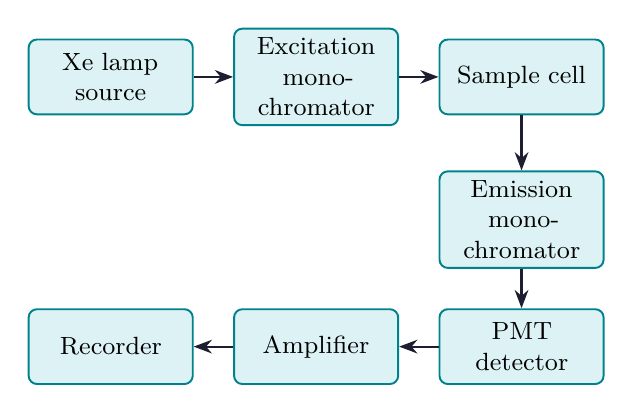
\begin{tikzpicture}[node distance=0.3cm and 0.45cm,
  sblock/.style={rectangle, draw=myteal, fill=hdrteal, text width=1.85cm,
    align=center, minimum height=0.95cm, font=\small,
    rounded corners=3pt, line width=0.7pt}]
  \node[sblock] (lamp) {Xe lamp source};
  \node[sblock, right=0.5cm of lamp] (mono1) {Excitation mono-chromator};
  \node[sblock, right=0.5cm of mono1] (cell) {Sample cell};
  \node[sblock, below=0.7cm of cell] (mono2) {Emission mono-chromator};
  \node[sblock, below=0.5cm of mono2] (det) {PMT detector};
  \node[sblock, left=0.5cm of det] (amp) {Amplifier};
  \node[sblock, left=0.5cm of amp] (rec) {Recorder};

  \draw[arrow] (lamp) -- (mono1);
  \draw[arrow] (mono1) -- (cell);
  \draw[arrow] (cell) -- (mono2);
  \draw[arrow] (mono2) -- (det);
  \draw[arrow] (det) -- (amp);
  \draw[arrow] (amp) -- (rec);
\end{tikzpicture}
\end{tcolorbox}

\subsection{Applications in Medicine and Biology}
Because fluorescence detection can sense single molecules, it has revolutionised diagnostics and therapy. The main medical applications are listed below.

\begin{tabularx}{\linewidth}{|B{3.4cm}|Y|}
\hline
\textbf{Application} & \textbf{How fluorescence is used} \\
\hline
Clinical assays (immunoassay) & Antibodies tagged with fluorescein/rhodamine bind specific antigens; concentration is read from fluorescence intensity (e.g.\ FIA, FACS). \\
\hline
DNA / RNA detection & Intercalating dyes (ethidium bromide, SYBR Green) and fluorescent probes used in gel imaging and \emph{quantitative} real-time PCR. \\
\hline
Fluorescence microscopy & GFP-tagged proteins visualised inside living cells; reveals localisation and dynamics. \\
\hline
Fluorescent angiography & Sodium fluorescein injected intravenously; ophthalmologist captures retinal vasculature images. \\
\hline
Cancer detection / surgery & 5-Aminolaevulinic acid (5-ALA) accumulates as fluorescent protoporphyrin IX in glioma cells; surgeon visualises tumour boundary in blue light. \\
\hline
Photodynamic therapy (PDT) & Light excites a porphyrin photosensitiser; via ISC it generates singlet oxygen which destroys tumour cells. \\
\hline
Pulse oximetry-related & Near-IR fluorescent probes monitor oxygenation; complementary to absorption oximetry. \\
\hline
Drug binding studies & Tryptophan in proteins (intrinsic fluorophore) reports drug-binding through quenching of its $340\ \mathrm{nm}$ band. \\
\hline
Biosensors & Fluorescence quenching of conjugated polymers used in glucose, $\mathrm{Ca^{2+}}$ and pH sensing. \\
\hline
\end{tabularx}

\begin{tcolorbox}[examplebox, title={Solved Example: Stern--Volmer Plot Reading}]
\textbf{Problem:} A fluorescence quenching experiment gives the following data:
\[
[Q] = 0,\,1,\,2\,\mathrm{mM};\quad F = 100,\,67,\,50\ \text{(arb.)}
\]
Find $K_{SV}$.

\textbf{Solution:} Compute $F_0/F$ for each $[Q]$:
\[
F_0/F = 1.00,\,1.49,\,2.00 \ \Rightarrow\ \text{slope}\approx 0.5\ \mathrm{mM^{-1}}
\]
\[
K_{SV}=500\ \mathrm{M^{-1}}
\]
A linear plot confirms purely collisional (dynamic) quenching.
\end{tcolorbox}

\begin{tcolorbox}[masonbox, title={Why Heavy Atoms and Oxygen Quench Fluorescence}]
Heavy atoms (Br, I) and dissolved $\mathrm{O_2}$ promote inter-system crossing $S_1\to T_1$. Once a molecule is in the triplet state, fluorescence is no longer possible. This ``heavy-atom effect'' is the basis of phosphorescent compounds, and the reason why deoxygenation is needed for high-quantum-yield emission measurements.
\end{tcolorbox}

\subsection{Kasha's Rule}
\begin{tcolorbox}[defbox]
\textbf{Kasha's rule:} Emission (fluorescence or phosphorescence) almost always occurs from the \emph{lowest} excited state of a given multiplicity, regardless of which higher state was initially populated by the absorbed photon.
\end{tcolorbox}

\textbf{Why it matters:}
\begin{itemize}[leftmargin=*, itemsep=2pt, topsep=2pt]
  \item Internal conversion $S_n \to S_1$ is much faster than $S_1 \to S_0$ fluorescence.
  \item The fluorescence wavelength is therefore independent of the excitation wavelength.
  \item This is why an excitation spectrum (intensity vs $\lambda_{\mathrm{exc}}$) reproduces the absorption spectrum exactly.
  \item Combined with the Franck--Condon principle (Section 1.7), it gives the mirror-image rule.
\end{itemize}

\subsection{Lifetime, Quantum Yield, and Radiative Rate}
The radiative lifetime $\tau_F$ and quantum yield $\Phi_F$ are not independent — they jointly fix the natural radiative rate $k_F$.

\begin{tcolorbox}[formulabox, title={Lifetime--Quantum Yield Connection}]
\[
\tau_F=\frac{1}{k_F+k_{NR}+k_{ISC}}, \qquad \Phi_F=k_F\,\tau_F
\]
The natural (radiative) lifetime is $\tau_0=1/k_F=\tau_F/\Phi_F$.\\
A short measured $\tau_F$ together with low $\Phi_F$ indicates strong non-radiative deactivation.
\end{tcolorbox}

\textbf{Diagnostic use:} Time-resolved fluorimetry measures $\tau_F$ directly. Combined with the steady-state $\Phi_F$, you can separate radiative ($k_F$) from non-radiative ($k_{NR}+k_{ISC}$) contributions and identify the dominant decay pathway.

\subsection{F\"orster Resonance Energy Transfer (FRET)}
FRET is non-radiative dipole--dipole energy transfer from an excited donor (D$^{*}$) to a nearby ground-state acceptor (A). The efficiency depends very strongly on the donor--acceptor distance, making FRET a ``spectroscopic ruler'' on the $1$--$10\ \mathrm{nm}$ scale.

\begin{tcolorbox}[formulabox, title={FRET Efficiency}]
\[
E=\frac{R_0^{6}}{R_0^{6}+r^{6}}=1-\frac{\tau_{DA}}{\tau_D}
\]
$r$ = donor--acceptor distance; $R_0$ = F\"orster radius (typically $1$--$10\ \mathrm{nm}$, the distance at which $E=50\%$); $\tau_D$ and $\tau_{DA}$ are donor lifetimes alone and in presence of acceptor.\\
Conditions: spectral overlap of donor emission and acceptor absorption; favourable orientation; $r$ within $\sim 2 R_0$.
\end{tcolorbox}

\begin{tcolorbox}[tikzbox, title={FRET: Donor and Acceptor Spectral Overlap}]
\centering
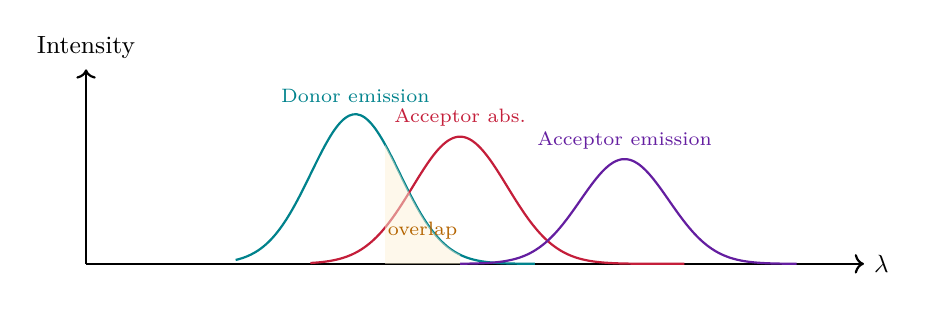
\begin{tikzpicture}[scale=0.95]
  \draw[->, thick] (0,0) -- (10.4,0) node[right, font=\small] {$\lambda$};
  \draw[->, thick] (0,0) -- (0,2.6) node[above, font=\small] {Intensity};
  % Donor emission (teal)
  \draw[myteal, thick, domain=2:6, samples=80, smooth, variable=\x] plot ({\x},{2.0*exp(-((\x-3.6)^2)/0.7)});
  \node[font=\scriptsize, color=myteal] at (3.6,2.25) {Donor emission};
  % Acceptor absorption (red, overlapping)
  \draw[myred, thick, domain=3:8, samples=80, smooth, variable=\x] plot ({\x},{1.7*exp(-((\x-5.0)^2)/0.8)});
  \node[font=\scriptsize, color=myred] at (5.0,1.95) {Acceptor abs.};
  % Acceptor emission (purple, far right)
  \draw[mypurple, thick, domain=5:9.5, samples=80, smooth, variable=\x] plot ({\x},{1.4*exp(-((\x-7.2)^2)/0.7)});
  \node[font=\scriptsize, color=mypurple] at (7.2,1.65) {Acceptor emission};
  % Overlap shading
  \fill[hdramber, opacity=0.5, domain=4:5, variable=\x]
       plot ({\x},{2.0*exp(-((\x-3.6)^2)/0.7)}) -- (5,0) -- (4,0) -- cycle;
  \node[font=\scriptsize, color=myamber] at (4.5,0.45) {overlap};
\end{tikzpicture}
\end{tcolorbox}

\textbf{Medical and biological applications of FRET:}
\begin{itemize}[leftmargin=*, itemsep=1pt, topsep=2pt]
  \item Protein conformational changes (label two residues with D and A).
  \item DNA hybridisation assays and SNP detection.
  \item Real-time PCR with TaqMan probes.
  \item Single-molecule FRET to track folding/binding kinetics.
  \item Fluorescent biosensors for $\mathrm{Ca^{2+}}$, $\mathrm{Zn^{2+}}$, ATP, kinase activity.
\end{itemize}

\begin{tcolorbox}[exambox, title={Exam Points (Section 3)}]
\begin{itemize}[leftmargin=*, itemsep=2pt, topsep=2pt]
  \item Always draw the Jablonski diagram first; mark $S_0, S_1, T_1$, IC, ISC, F, P.
  \item Stokes shift = ``vibrational relaxation before emission''.
  \item Compare F and P using a 4-row table.
  \item Medicine answer must include \emph{at least three} applications: fluorescein angiography, PDT, FIA.
  \item State Kasha's rule and link it to the wavelength-independence of emission.
  \item FRET efficiency $E = R_0^6/(R_0^6+r^6)$ — the $r^{-6}$ distance dependence is the standard 5-mark question.
\end{itemize}
\end{tcolorbox}

% ===============================================================================
\section{Vibrational and Rotational Spectroscopy of Diatomic Molecules}
% ===============================================================================

\begin{tcolorbox}[defbox]
A diatomic molecule rotates about its centre of mass and vibrates along its bond. Photon absorption in the microwave region excites pure rotation; absorption in the infrared region excites vibration (often together with simultaneous rotational changes). Together these tell us bond length, bond strength, force constant, and moment of inertia.
\end{tcolorbox}

\subsection{Rotational Spectroscopy: The Rigid-Rotor Model}
The molecule is modelled as two masses $m_1$ and $m_2$ joined by a rigid rod of length $r$ (the bond length). The reduced mass is
\[
\mu=\frac{m_1 m_2}{m_1+m_2}
\]
and the moment of inertia about the centre of mass is
\[
I=\mu r^{2}
\]

\begin{tcolorbox}[formulabox, title={Rotational Energy Levels (Rigid Rotor)}]
\[
E_J = \frac{\hbar^{2}}{2I}\,J(J+1) \quad\text{or}\quad \tilde{E}_J=\bar{B}\,J(J+1)\ \mathrm{cm^{-1}}
\]
where $J=0,1,2,\ldots$ is the rotational quantum number and the rotational constant is
\[
\bar{B}=\frac{h}{8\pi^{2} c\, I}\ \mathrm{cm^{-1}}
\]
\textbf{Selection rule:} $\Delta J=\pm 1$, and the molecule must possess a permanent dipole moment.
\end{tcolorbox}

\textbf{Spacing of allowed transitions:} For absorption $J\to J+1$,
\[
\Delta\tilde{E}=\tilde{E}_{J+1}-\tilde{E}_{J}=2\bar{B}(J+1)
\]
so successive lines are separated by a constant $2\bar{B}$. From this spacing one can compute $I$, then $r$.

\begin{tcolorbox}[tikzbox, title={Rotational Energy Levels and Spectrum}]
\centering
\begin{tikzpicture}[scale=0.95]
  % Energy ladder
  \foreach \J/\y in {0/0, 1/0.4, 2/1.2, 3/2.4, 4/4.0} {
     \draw[thick, mydark] (0,\y) -- (3.0,\y) node[right, font=\scriptsize] {$J=\J$};
  }
  % Transitions
  \draw[redarrow] (0.4,0)   -- (0.4,0.38);
  \draw[redarrow] (0.9,0.4) -- (0.9,1.18);
  \draw[redarrow] (1.4,1.2) -- (1.4,2.38);
  \draw[redarrow] (1.9,2.4) -- (1.9,3.98);

  % Stick spectrum on right
  \draw[->, thick] (4.6,0) -- (10.6,0) node[right, font=\small] {$\bar{\nu}$};
  \foreach \x/\h in {5.4/1.0, 6.4/1.0, 7.4/1.0, 8.4/1.0, 9.4/1.0} \draw[thick, myteal] (\x,0)--(\x,\h);
  \node[font=\scriptsize] at (5.4,-0.35) {$2\bar{B}$};
  \node[font=\scriptsize] at (6.4,-0.35) {$4\bar{B}$};
  \node[font=\scriptsize] at (7.4,-0.35) {$6\bar{B}$};
  \node[font=\scriptsize] at (8.4,-0.35) {$8\bar{B}$};
  \node[font=\scriptsize] at (9.4,-0.35) {$10\bar{B}$};
\end{tikzpicture}
\end{tcolorbox}

\begin{tcolorbox}[examplebox, title={Solved Example: Bond Length of HCl from Rotational Spectrum}]
\textbf{Problem:} For HCl, $\bar{B}=10.59\ \mathrm{cm^{-1}}$. Calculate the H--Cl bond length. Take $\mu_{\mathrm{HCl}}=1.628\times10^{-27}\ \mathrm{kg}$.

\textbf{Solution:} From $\bar{B}=h/(8\pi^{2}cI)$,
\[
I=\frac{h}{8\pi^{2}c\bar{B}}=\frac{6.626\times10^{-34}}{8\pi^{2}\times 3\times10^{10}\times 10.59}=2.64\times10^{-47}\ \mathrm{kg\,m^{2}}
\]
Using $I=\mu r^{2}$,
\[
r=\sqrt{\frac{I}{\mu}}=\sqrt{\frac{2.64\times10^{-47}}{1.628\times10^{-27}}}=1.27\times10^{-10}\ \mathrm{m}=127\ \mathrm{pm}
\]
\textbf{Result:} The H--Cl bond length is $\approx 127\ \mathrm{pm}$.
\end{tcolorbox}

\subsection{Vibrational Spectroscopy: Simple Harmonic Oscillator Model}
For small displacements the bond can be modelled as a Hookean spring with force constant $k$. Its quantised energies are
\[
E_v=\left(v+\tfrac{1}{2}\right)h\nu_0,\quad v=0,1,2,\ldots,\quad \nu_0=\frac{1}{2\pi}\sqrt{\frac{k}{\mu}}
\]
The fundamental absorption is the $v{=}0\to v{=}1$ transition.

\begin{tcolorbox}[formulabox, title={Vibrational Frequency and Wavenumber}]
\[
\bar{\nu}_0=\frac{1}{2\pi c}\sqrt{\frac{k}{\mu}}\ \mathrm{cm^{-1}}
\]
\textbf{Selection rule:} $\Delta v=\pm 1$ for harmonic oscillator (gross rule: vibration must change the dipole moment).\\
\textbf{Zero-point energy:} $E_0=\tfrac12 h\nu_0\neq 0$, even at $0\ \mathrm{K}$.
\end{tcolorbox}

\begin{tcolorbox}[tikzbox, title={Harmonic Oscillator and Anharmonic (Morse) Potential}]
\centering
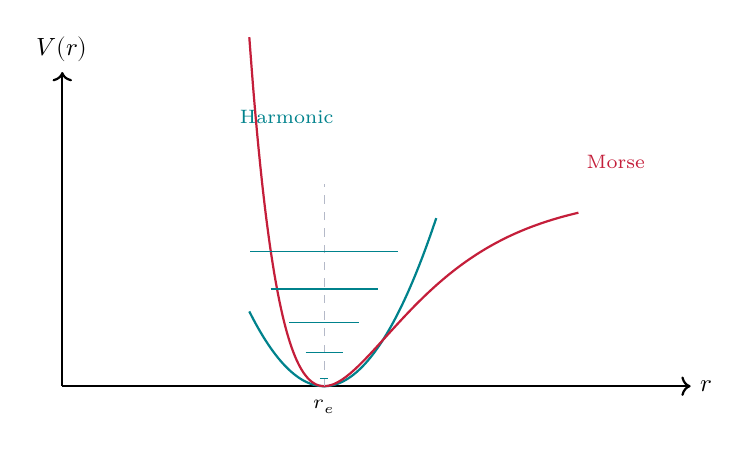
\begin{tikzpicture}[scale=0.95]
  % axes
  \draw[->, thick] (0,0) -- (8.4,0) node[right, font=\small] {$r$};
  \draw[->, thick] (0,0) -- (0,4.2) node[above, font=\small] {$V(r)$};
  % harmonic parabola
  \draw[myteal, thick, domain=-1.0:1.5, samples=80, smooth, variable=\x] plot ({\x+3.5},{(\x)^2});
  \node[font=\scriptsize, color=myteal] at (3.0,3.6) {Harmonic};
  % Morse curve
  \draw[myred, thick, domain=-1.0:3.4, samples=80, smooth, variable=\x] plot ({\x+3.5}, {2.6*(1-exp(-0.85*\x))^2});
  \node[font=\scriptsize, color=myred] at (7.4,3.0) {Morse};
  % equilibrium
  \draw[dashed, mgframe] (3.5,0) -- (3.5,2.7);
  \node[font=\scriptsize, anchor=north] at (3.5,-0.05) {$r_e$};
  % vibrational levels (harmonic)
  \foreach \v/\y in {0/0.10, 1/0.45, 2/0.85, 3/1.30, 4/1.80} {
     \draw[thin, myteal] (3.5-\y*0.55,\y) -- (3.5+\y*0.55,\y);
  }
\end{tikzpicture}
\end{tcolorbox}

\textbf{Anharmonicity (Morse) corrections:}\par\noindent
\begin{tabularx}{\linewidth}{|B{3.6cm}|Y|}
\hline
\textbf{Feature} & \textbf{Effect} \\
\hline
Levels not equally spaced & Spacing decreases as $v$ increases. \\
\hline
Selection rule modified & Overtones $\Delta v=\pm 2,\pm 3,\ldots$ become weakly allowed. \\
\hline
Bond dissociation possible & At sufficient $v$, vibration breaks the bond. \\
\hline
Energy expression & $\tilde{E}_v=\bar{\nu}_e(v+\tfrac12)-\bar{\nu}_e x_e (v+\tfrac12)^{2}$ \\
\hline
\end{tabularx}

\subsection{Vibration--Rotation (Rovibrational) Spectra of Diatomics}
A vibrational transition is usually accompanied by a change in $J$. The fundamental band of HCl, for example, shows a P-branch ($\Delta J=-1$) and an R-branch ($\Delta J=+1$) but \emph{no} central Q-branch ($\Delta J=0$).

\begin{tcolorbox}[tikzbox, title={Rovibrational Spectrum: P and R Branches}]
\centering
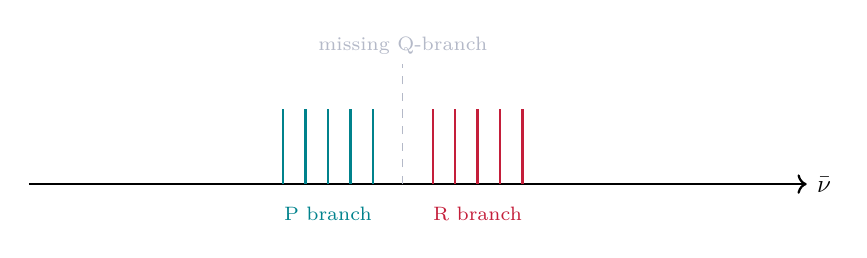
\begin{tikzpicture}[scale=0.95]
  \draw[->, thick] (0,0) -- (10.4,0) node[right, font=\small] {$\bar{\nu}$};
  \draw[dashed, mgframe] (5.0,0) -- (5.0,1.6);
  \node[font=\scriptsize, color=mgframe] at (5.0,1.85) {missing Q-branch};
  % P-branch
  \foreach \x in {3.4, 3.7, 4.0, 4.3, 4.6} \draw[thick, myteal] (\x,0)--(\x,1.0);
  \node[font=\scriptsize, color=myteal] at (4.0,-0.4) {P branch};
  % R-branch
  \foreach \x in {5.4, 5.7, 6.0, 6.3, 6.6} \draw[thick, myred] (\x,0)--(\x,1.0);
  \node[font=\scriptsize, color=myred] at (6.0,-0.4) {R branch};
\end{tikzpicture}
\end{tcolorbox}

\subsection{Modes of Vibration in Polyatomic Molecules}
A non-linear molecule with $N$ atoms has $3N-6$ vibrational modes; a linear one has $3N-5$ modes. Each mode is either stretching (along the bond) or bending (across the bond).

\begin{tcolorbox}[tikzbox, title={Stretching and Bending Vibrations}]
\centering
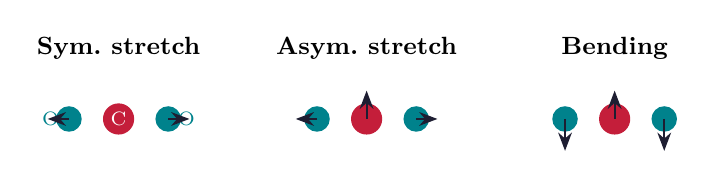
\begin{tikzpicture}[scale=0.9]
  % Symmetric stretch
  \node[font=\small\bfseries] at (1.0,2.0) {Sym.\ stretch};
  \fill[myteal] (0.3,1.0) circle (0.18) node[anchor=east, font=\scriptsize] {O};
  \fill[myred]  (1.0,1.0) circle (0.22) node[font=\scriptsize, color=white] {C};
  \fill[myteal] (1.7,1.0) circle (0.18) node[anchor=west, font=\scriptsize] {O};
  \draw[arrow] (0.3,1.0)--(0.0,1.0);
  \draw[arrow] (1.7,1.0)--(2.0,1.0);

  % Asymmetric stretch
  \node[font=\small\bfseries] at (4.5,2.0) {Asym.\ stretch};
  \fill[myteal] (3.8,1.0) circle (0.18);
  \fill[myred]  (4.5,1.0) circle (0.22);
  \fill[myteal] (5.2,1.0) circle (0.18);
  \draw[arrow] (3.8,1.0)--(3.5,1.0);
  \draw[arrow] (5.2,1.0)--(5.5,1.0);
  \draw[arrow] (4.5,1.0)--(4.5,1.4);

  % Bending
  \node[font=\small\bfseries] at (8.0,2.0) {Bending};
  \fill[myteal] (7.3,1.0) circle (0.18);
  \fill[myred]  (8.0,1.0) circle (0.22);
  \fill[myteal] (8.7,1.0) circle (0.18);
  \draw[arrow] (7.3,1.0)--(7.3,0.55);
  \draw[arrow] (8.7,1.0)--(8.7,0.55);
  \draw[arrow] (8.0,1.0)--(8.0,1.4);
\end{tikzpicture}
\end{tcolorbox}

\textbf{Number of modes for common molecules:}\par\noindent
\begin{tabularx}{\linewidth}{|B{2.6cm}|Y|Y|Y|}
\hline
\textbf{Molecule} & \textbf{Geometry} & \textbf{$3N-5$ or $3N-6$} & \textbf{Modes} \\
\hline
$\mathrm{CO_2}$ & Linear & $3(3)-5$ & 4 (sym str, asym str, two bends) \\
\hline
$\mathrm{H_2O}$ & Bent & $3(3)-6$ & 3 (sym str, asym str, scissor) \\
\hline
$\mathrm{NH_3}$ & Pyramidal & $3(4)-6$ & 6 \\
\hline
$\mathrm{CH_4}$ & Tetrahedral & $3(5)-6$ & 9 \\
\hline
\end{tabularx}

\subsection{Characteristic IR Group Frequencies}
A practical IR fingerprint table is essential for compound identification.

\begin{tabularx}{\linewidth}{|B{3.4cm}|Y|Y|}
\hline
\textbf{Group} & \textbf{Wavenumber (cm$^{-1}$)} & \textbf{Intensity / nature} \\
\hline
O--H (alcohol) & $3200$--$3550$ (broad) & Strong, broad due to H-bond \\
\hline
N--H (amine) & $3300$--$3500$ & Medium, sharp \\
\hline
C--H (sp$^{3}$) & $2850$--$2960$ & Strong \\
\hline
C--H (sp$^{2}$, aromatic) & $3000$--$3100$ & Medium \\
\hline
C${\equiv}$N & $2210$--$2260$ & Medium \\
\hline
C${\equiv}$C & $2100$--$2260$ & Weak \\
\hline
C${=}$O (ester, ketone) & $1680$--$1750$ & Very strong \\
\hline
C${=}$C & $1620$--$1680$ & Variable \\
\hline
N--O (NO$_2$) & $1300$--$1550$ (two bands) & Strong \\
\hline
C--O & $1000$--$1300$ & Strong \\
\hline
\end{tabularx}

\subsection{Block Diagram of an FT-IR Spectrometer}
Modern IR instruments use a Michelson interferometer and Fourier transform of the interferogram to obtain the spectrum.

\begin{tcolorbox}[tikzbox, title={Block Diagram of an FT-IR Spectrometer}]
\centering
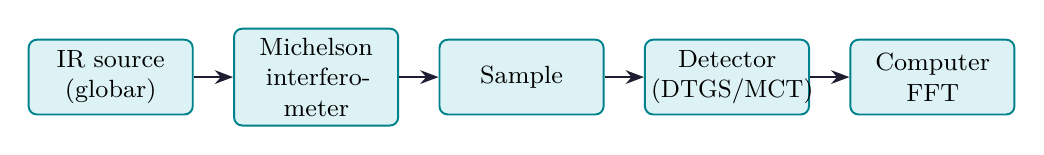
\begin{tikzpicture}[node distance=0.3cm and 0.45cm,
  sblock/.style={rectangle, draw=myteal, fill=hdrteal, text width=1.85cm,
    align=center, minimum height=0.95cm, font=\small,
    rounded corners=3pt, line width=0.7pt}]
  \node[sblock] (n1) {IR source\\(globar)};
  \node[sblock, right=0.5cm of n1] (n2) {Michelson interfero-meter};
  \node[sblock, right=0.5cm of n2] (n3) {Sample};
  \node[sblock, right=0.5cm of n3] (n4) {Detector\\(DTGS/MCT)};
  \node[sblock, right=0.5cm of n4] (n5) {Computer\\FFT};
  \draw[arrow] (n1)--(n2);
  \draw[arrow] (n2)--(n3);
  \draw[arrow] (n3)--(n4);
  \draw[arrow] (n4)--(n5);
\end{tikzpicture}
\end{tcolorbox}

\subsection{Applications of IR and Microwave Spectroscopy}
\begin{itemize}[leftmargin=*, itemsep=2pt, topsep=2pt]
  \item Identification of functional groups (most common organic-chem application).
  \item Distinguishing isomers (e.g.\ acetone vs propanal by C${=}$O stretch position).
  \item Hydrogen bonding studies through O--H shift.
  \item Quantitative analysis using calibrated absorbance.
  \item Microwave spectroscopy gives bond lengths and bond angles to better than $0.1\ \mathrm{pm}$.
  \item Pollution monitoring: IR detects $\mathrm{CO}, \mathrm{CO_2}, \mathrm{NO_x}, \mathrm{SO_2}$ in stack gas.
  \item Polymer/coating analysis (ATR-IR).
\end{itemize}

\subsection{Centrifugal Distortion of the Rigid Rotor}
At higher rotational levels the bond stretches slightly under centrifugal force, increasing the moment of inertia and reducing the spacing between successive lines. The corrected energy expression is
\[
\tilde{E}_J = \bar{B}\,J(J+1) - \bar{D}\,J^{2}(J+1)^{2}
\]
where $\bar{D}$ is the centrifugal-distortion constant ($\bar{D}\ll \bar{B}$). This makes high-$J$ lines slightly closer than the rigid-rotor prediction of $2\bar{B}$ spacing.

\subsection{Isotope Effect on Vibrational and Rotational Spectra}
Replacing $\mathrm{H}$ by $\mathrm{D}$ doubles the reduced mass without changing the force constant. This is a standard MAKAUT viva question and a standard 5-mark numerical.

\begin{tcolorbox}[formulabox, title={Effect of Isotopic Substitution}]
Since $\bar{\nu}_0=(1/2\pi c)\sqrt{k/\mu}$ and $k$ is unchanged,
\[
\frac{\bar{\nu}_{\mathrm{D}}}{\bar{\nu}_{\mathrm{H}}}=\sqrt{\frac{\mu_{\mathrm{H}}}{\mu_{\mathrm{D}}}}\approx \frac{1}{\sqrt{2}}\approx 0.71
\]
For rotational spectra, $\bar{B}\propto 1/\mu r^{2}$, so heavier isotopes give smaller $\bar{B}$ and tighter line spacing.
\end{tcolorbox}

\begin{tcolorbox}[examplebox, title={Solved Example: \texorpdfstring{$\mathrm{H{-}Cl}$}{H-Cl} vs \texorpdfstring{$\mathrm{D{-}Cl}$}{D-Cl} Vibrational Frequency}]
For HCl, $\bar{\nu}_0 \approx 2989\ \mathrm{cm^{-1}}$. Predict $\bar{\nu}_0$ for DCl.\\
The reduced masses are $\mu_{\mathrm{HCl}}=0.972\ \mathrm{u}$ and $\mu_{\mathrm{DCl}}=1.904\ \mathrm{u}$.
\[
\bar{\nu}_{\mathrm{DCl}}=\bar{\nu}_{\mathrm{HCl}}\sqrt{\frac{\mu_{\mathrm{HCl}}}{\mu_{\mathrm{DCl}}}}=2989\sqrt{\frac{0.972}{1.904}}=2989\times 0.715=2137\ \mathrm{cm^{-1}}
\]
Observed value: $2145\ \mathrm{cm^{-1}}$ — excellent agreement.
\end{tcolorbox}

\subsection{Fingerprint Region vs Functional-Group Region}
The IR spectrum is conventionally divided into two regions, and they are used differently in identification.

\begin{tabularx}{\linewidth}{|B{2.8cm}|Y|Y|}
\hline
\textbf{Region} & \textbf{Range (cm$^{-1}$)} & \textbf{Use} \\
\hline
Functional-group region & $4000$--$1500$ & Quick identification of common groups (O--H, N--H, C--H, C${=}$O, C${\equiv}$N, etc.). \\
\hline
Fingerprint region & $1500$--$400$ & Highly specific to the whole molecule; used to confirm identity by comparison with a reference spectrum. Do not assign every peak; match the overall pattern. \\
\hline
\end{tabularx}

\subsection{Sample Preparation for IR Spectroscopy}
The right method depends on the physical state of the sample.

\begin{tabularx}{\linewidth}{|B{2.8cm}|Y|Y|}
\hline
\textbf{Sample} & \textbf{Method} & \textbf{Notes} \\
\hline
Solid (crystalline) & KBr pellet & 1\,\% sample in dry KBr, pressed at $10\ \mathrm{tonnes}$; KBr is IR-transparent above $400\ \mathrm{cm^{-1}}$. \\
\hline
Solid (amorphous) & Nujol mull & Mineral oil paste between two NaCl plates. Nujol bands at $\sim 2900, 1460, 1380\ \mathrm{cm^{-1}}$ — ignore them. \\
\hline
Liquid (neat) & Capillary film & Single drop between two NaCl windows. \\
\hline
Liquid (dilute) & Solution cell & $\mathrm{CCl_4}$, $\mathrm{CHCl_3}$, or $\mathrm{CS_2}$ — all transparent in different ranges. \\
\hline
Gas & Long-path gas cell & $5$--$10\ \mathrm{cm}$ path, NaCl/KBr windows. \\
\hline
Surface / film & ATR (attenuated total reflectance) & No prep needed; press sample on Ge/diamond crystal. \\
\hline
\end{tabularx}

\subsection{IR vs Raman: Side-by-Side Comparison}
\begin{tabularx}{\linewidth}{|B{2.8cm}|Y|Y|}
\hline
\textbf{Feature} & \textbf{IR} & \textbf{Raman} \\
\hline
Photon process & Absorption & Inelastic scattering \\
\hline
Gross selection rule & Vibration must change \emph{dipole} & Vibration must change \emph{polarisability} \\
\hline
Strongest for & Polar bonds (O--H, C${=}$O) & Symmetric, non-polar bonds (C${=}$C, S--S) \\
\hline
Water as solvent & Bad (water absorbs strongly) & Excellent (water is a weak Raman scatterer) \\
\hline
Sample prep & KBr pellet, mull, ATR & Almost none; can be in glass capillary \\
\hline
Source & IR globar & Visible / NIR laser \\
\hline
Sensitivity & High & Low (only $\sim 10^{-7}$ of incident photons scattered) \\
\hline
\end{tabularx}

\begin{tcolorbox}[exambox, title={Exam Points (Section 4)}]
\begin{itemize}[leftmargin=*, itemsep=2pt, topsep=2pt]
  \item Quote both the gross rule (dipole change) and specific rule ($\Delta v=\pm1$) for IR.
  \item For numericals: $\bar{B}=h/(8\pi^{2}cI)$ and $\bar{\nu}_0=(1/2\pi c)\sqrt{k/\mu}$.
  \item Mention zero-point energy as a quantum effect.
  \item For polyatomic, give $3N-6$ / $3N-5$ rule with $\mathrm{H_2O}$/$\mathrm{CO_2}$ example.
  \item Always cite C${=}$O ($\sim 1700\ \mathrm{cm^{-1}}$) and O--H ($\sim 3400\ \mathrm{cm^{-1}}$) bands.
  \item Isotope shift $\bar{\nu}_{\mathrm{D}}/\bar{\nu}_{\mathrm{H}} \approx 1/\sqrt{2}$ for X--H vs X--D — standard 5-mark numerical.
  \item Sample prep choice: KBr pellet for solids, ATR for everything else.
  \item Fingerprint region $<1500\ \mathrm{cm^{-1}}$ confirms identity, functional-group region $>1500\ \mathrm{cm^{-1}}$ identifies groups.
\end{itemize}
\end{tcolorbox}

% ===============================================================================
\section{Nuclear Magnetic Resonance (NMR) and Magnetic Resonance Imaging (MRI)}
% ===============================================================================

\begin{tcolorbox}[defbox]
\textbf{Nuclear Magnetic Resonance (NMR)} is the absorption of radio-frequency radiation by nuclei placed in a strong magnetic field. Only nuclei with non-zero spin quantum number $I\neq 0$ are NMR-active (e.g.\ $^{1}\mathrm{H}, ^{13}\mathrm{C}, ^{19}\mathrm{F}, ^{31}\mathrm{P}$). The chemical environment of each nucleus modifies the resonance frequency and gives a structural fingerprint of the molecule.
\end{tcolorbox}

\subsection{Nuclear Spin and Magnetic Moment}
A nucleus with spin $I$ has a magnetic moment
\[
\vec{\mu}=\gamma\,\vec{I}\,\hbar
\]
where $\gamma$ is the magnetogyric ratio. In an external field $\vec{B}_0$, the spin can take $2I+1$ orientations of energy
\[
E_m=-\gamma m_I\hbar B_0,\qquad m_I=I, I-1,\ldots,-I
\]
For a $^{1}\mathrm{H}$ nucleus ($I=1/2$) only two states exist: $m_I=+1/2$ (lower, aligned with $B_0$) and $m_I=-1/2$ (higher, opposed).

\begin{tcolorbox}[formulabox, title={Larmor (Resonance) Condition}]
\[
\Delta E = \gamma\hbar B_0 = h\nu_L \quad\Rightarrow\quad \nu_L=\frac{\gamma B_0}{2\pi}
\]
$\nu_L$ is called the Larmor frequency. \textbf{Selection rule:} $\Delta m_I=\pm 1$.\\
For $^{1}\mathrm{H}$ in $B_0=11.74\ \mathrm{T}$, $\nu_L=500\ \mathrm{MHz}$.
\end{tcolorbox}

\subsection{Chemical Shift}
The local electron cloud shields each nucleus, so the actual field experienced is $B_{\mathrm{eff}}=B_0(1-\sigma)$, where $\sigma$ is the shielding constant. Different chemical environments have different $\sigma$, leading to slightly different resonance frequencies. To make the values instrument-independent, the chemical shift is referenced to TMS (tetramethylsilane).

\begin{tcolorbox}[formulabox, title={Chemical Shift}]
\[
\delta\ (\mathrm{ppm}) = \frac{\nu_{\mathrm{sample}}-\nu_{\mathrm{TMS}}}{\nu_{\mathrm{spectrometer}}}\times 10^{6}
\]
Higher $\delta$ = deshielded = downfield. Lower $\delta$ = shielded = upfield. TMS is set at $\delta=0\ \mathrm{ppm}$.
\end{tcolorbox}

\textbf{Typical $^{1}\mathrm{H}$ chemical shift ranges:}\par\noindent
\begin{tabularx}{\linewidth}{|B{3.4cm}|Y|Y|}
\hline
\textbf{Type of proton} & \textbf{$\delta$ (ppm)} & \textbf{Comment} \\
\hline
TMS & 0.0 & Reference standard \\
\hline
Alkyl C--H & 0.5--2.0 & Most shielded \\
\hline
Allylic / $\alpha$-carbonyl & 2.0--3.0 & Slight deshielding \\
\hline
$\mathrm{C{-}O{-}H}$, $\mathrm{C{-}O{-}CH}$ & 3.0--4.5 & Deshielded by O \\
\hline
Vinyl ($\mathrm{C{=}CH}$) & 4.5--6.5 & $\pi$-electron shielding \\
\hline
Aromatic & 6.5--8.5 & Ring current deshielding \\
\hline
Aldehyde ($\mathrm{CHO}$) & 9.0--10.0 & Strong deshielding by C${=}$O \\
\hline
Carboxylic acid OH & 10--13 (broad) & H-bonded, broad \\
\hline
\end{tabularx}

\subsection{Spin--Spin Coupling and Multiplicity}
Adjacent magnetic nuclei split each other's signals. The number of equivalent neighbours $n$ produces $n+1$ lines in a binomial intensity ratio (Pascal's triangle).

\begin{tcolorbox}[formulabox, title={\texorpdfstring{$n+1$}{n+1} Rule}]
\[
\text{multiplicity}=n+1
\]
where $n$ is the number of \emph{equivalent} neighbouring (vicinal) protons. The coupling constant $J$ is measured in Hz and is independent of $B_0$.
\end{tcolorbox}

\textbf{Common multiplets:}\par\noindent
\begin{tabularx}{\linewidth}{|B{2.4cm}|Y|Y|Y|}
\hline
\textbf{$n$ neighbours} & \textbf{Pattern} & \textbf{Intensity ratio} & \textbf{Example} \\
\hline
0 & Singlet & 1 & $\mathrm{(CH_3)_4Si}$ \\
\hline
1 & Doublet & 1:1 & CHCl$_2$--CH (coupled to 1H) \\
\hline
2 & Triplet & 1:2:1 & CH$_3$--CH$_2$--X \\
\hline
3 & Quartet & 1:3:3:1 & X--CH$_2$--CH$_3$ \\
\hline
6 & Septet & 1:6:15:20:15:6:1 & Isopropyl CH \\
\hline
\end{tabularx}

\begin{tcolorbox}[examplebox, title={Solved Example: NMR of Ethanol (\texorpdfstring{$\mathrm{CH_3CH_2OH}$}{CH3CH2OH})}]
\textbf{Three sets of equivalent protons:}
\begin{itemize}[leftmargin=*, itemsep=1pt, topsep=2pt]
  \item $\mathrm{CH_3}$ : $\delta\approx 1.2\ \mathrm{ppm}$, \textbf{triplet} (coupled to 2 CH$_2$ neighbours).
  \item $\mathrm{CH_2}$ : $\delta\approx 3.7\ \mathrm{ppm}$, \textbf{quartet} (coupled to 3 CH$_3$ neighbours).
  \item $\mathrm{OH}$ : $\delta\approx 2.6\ \mathrm{ppm}$, broad \textbf{singlet} (rapid exchange averages coupling).
\end{itemize}
Integration ratio: $3:2:1$, exactly matching the proton counts.
\end{tcolorbox}

\subsection{Block Diagram of an NMR Spectrometer}
Modern instruments are pulsed Fourier-transform spectrometers (FT-NMR), which excite all nuclei simultaneously with a strong RF pulse and detect the free-induction decay (FID).

\begin{tcolorbox}[tikzbox, title={Block Diagram of FT-NMR}]
\centering
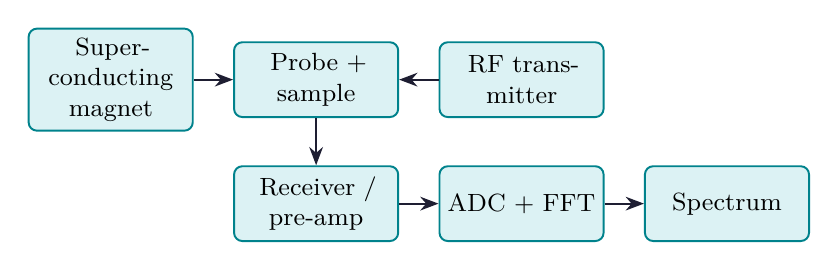
\begin{tikzpicture}[node distance=0.3cm and 0.45cm,
  sblock/.style={rectangle, draw=myteal, fill=hdrteal, text width=1.85cm,
    align=center, minimum height=0.95cm, font=\small,
    rounded corners=3pt, line width=0.7pt}]
  \node[sblock] (mag)  {Super-conducting magnet};
  \node[sblock, right=0.5cm of mag]  (probe) {Probe + sample};
  \node[sblock, right=0.5cm of probe] (rf)   {RF transmitter};
  \node[sblock, below=0.6cm of probe] (rec)  {Receiver / pre-amp};
  \node[sblock, right=0.5cm of rec]  (adc)  {ADC + FFT};
  \node[sblock, right=0.5cm of adc]  (disp) {Spectrum};
  \draw[arrow] (rf) -- (probe);
  \draw[arrow] (mag) -- (probe);
  \draw[arrow] (probe) -- (rec);
  \draw[arrow] (rec) -- (adc);
  \draw[arrow] (adc) -- (disp);
\end{tikzpicture}
\end{tcolorbox}

\subsection{Applications of NMR}
\begin{itemize}[leftmargin=*, itemsep=2pt, topsep=2pt]
  \item Structural elucidation of organic compounds (number of H environments, connectivity, stereochemistry).
  \item Molecular dynamics: relaxation times $T_1$ and $T_2$ probe motion.
  \item Quantitative NMR (qNMR) for drug purity certification.
  \item Solid-state NMR (MAS) for polymers, batteries, and materials.
  \item Protein structure determination via 2D NOESY/HSQC.
\end{itemize}

\subsection{Magnetic Resonance Imaging (MRI)}
MRI applies the principles of NMR to image the inside of the human body without ionising radiation.

\begin{tcolorbox}[defbox]
\textbf{MRI} produces tomographic images by spatially encoding the NMR signal of water protons in the body using \emph{magnetic field gradients}, then reconstructing the image by Fourier transform.
\end{tcolorbox}

\textbf{Why protons?} The body contains $\sim 60$--$70\%$ water, providing an abundant $^{1}\mathrm{H}$ signal. Different tissues differ in (i) proton density, (ii) longitudinal relaxation time $T_1$, and (iii) transverse relaxation time $T_2$ — the key contrast parameters.

\begin{tcolorbox}[formulabox, title={Spatial Encoding using Gradient Fields}]
A linear gradient $G_z=\partial B/\partial z$ makes the resonance frequency of a proton depend on its position $z$:
\[
\nu(z)=\frac{\gamma}{2\pi}\,\bigl(B_0 + G_z\,z\bigr)
\]
Combining $x, y, z$ gradients with phase and frequency encoding produces a 2D or 3D image.
\end{tcolorbox}

\begin{tcolorbox}[tikzbox, title={Major Components of an MRI Scanner}]
\centering
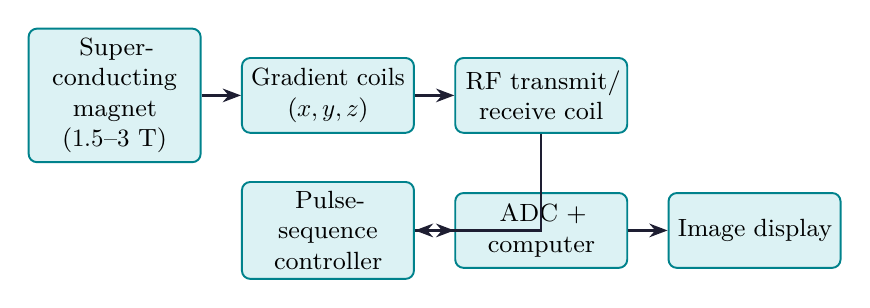
\begin{tikzpicture}[node distance=0.3cm and 0.45cm,
  sblock/.style={rectangle, draw=myteal, fill=hdrteal, text width=1.95cm,
    align=center, minimum height=0.95cm, font=\small,
    rounded corners=3pt, line width=0.7pt}]
  \node[sblock] (n1) {Super-conducting magnet ($1.5$--$3\ \mathrm{T}$)};
  \node[sblock, right=0.5cm of n1] (n2) {Gradient coils\\($x,y,z$)};
  \node[sblock, right=0.5cm of n2] (n3) {RF transmit/ receive coil};
  \node[sblock, below=0.6cm of n2] (n4) {Pulse-sequence controller};
  \node[sblock, right=0.5cm of n4] (n5) {ADC +\\computer};
  \node[sblock, right=0.5cm of n5] (n6) {Image display};
  \draw[arrow] (n1)--(n2);
  \draw[arrow] (n2)--(n3);
  \draw[arrow] (n3) |- (n4);
  \draw[arrow] (n4)--(n5);
  \draw[arrow] (n5)--(n6);
\end{tikzpicture}
\end{tcolorbox}

\subsection{T\texorpdfstring{$_1$}{1} and T\texorpdfstring{$_2$}{2} Contrast}
\begin{tabularx}{\linewidth}{|B{3.0cm}|Y|Y|}
\hline
\textbf{Image type} & \textbf{Contrast source} & \textbf{Tissue look} \\
\hline
$T_1$-weighted & Short TR, short TE; differences in spin--lattice relaxation & Fat is bright, water (CSF) is dark \\
\hline
$T_2$-weighted & Long TR, long TE; differences in spin--spin relaxation & Water is bright, fat is intermediate \\
\hline
Proton density & Long TR, short TE & Reflects total $^{1}\mathrm{H}$ count \\
\hline
fMRI (BOLD) & Magnetic susceptibility change of haemoglobin & Detects neural activity \\
\hline
\end{tabularx}

\subsection{Advantages and Limitations of MRI}
\begin{tabularx}{\linewidth}{|B{3.0cm}|Y|Y|}
\hline
\textbf{Aspect} & \textbf{Advantages} & \textbf{Limitations} \\
\hline
Radiation & Non-ionising, safe & --- \\
\hline
Soft-tissue contrast & Excellent (best of all imaging modalities) & --- \\
\hline
Cost & --- & Very expensive scanner and cryogen \\
\hline
Acquisition time & --- & Several minutes per sequence \\
\hline
Patient compatibility & --- & Pacemakers, ferromagnetic implants, claustrophobia \\
\hline
\end{tabularx}

\subsection{Medical Applications of MRI}
\begin{itemize}[leftmargin=*, itemsep=2pt, topsep=2pt]
  \item Brain: tumour detection, multiple sclerosis, stroke (diffusion MRI).
  \item Spinal cord and joints: disc prolapse, ligament tears.
  \item Cardiac MRI: chamber size, ejection fraction, myocardial viability.
  \item Functional MRI (fMRI): mapping of brain activity using BOLD contrast.
  \item Magnetic resonance angiography (MRA) without iodinated contrast.
  \item Whole-body screening and oncology staging.
\end{itemize}

\subsection{Origin of Chemical Shift: Shielding Mechanisms}
A nucleus's resonance frequency is determined by the local field $B_{\mathrm{eff}}=B_0(1-\sigma)$. The shielding constant $\sigma$ has three additive contributions in organic molecules.

\begin{tabularx}{\linewidth}{|B{3.4cm}|Y|}
\hline
\textbf{Mechanism} & \textbf{Effect} \\
\hline
Diamagnetic shielding ($\sigma_d$) & Local circulation of bonding electrons opposes $B_0$. Increases with electron density on the nucleus. Electronegative neighbours \emph{decrease} $\sigma_d$ and shift signal downfield. \\
\hline
Paramagnetic shielding ($\sigma_p$) & Mixing of low-lying excited states with the ground state \emph{adds} to $B_{\mathrm{eff}}$ and shifts signal downfield. Important in $^{13}\mathrm{C}$ but small in $^{1}\mathrm{H}$. \\
\hline
Anisotropic / ring-current shielding & Aromatic $\pi$-electrons circulate in $B_0$, generating a secondary field. Protons \emph{above/below} the ring are shielded; protons \emph{at the edge} are deshielded ($\delta\sim 7$--$8\ \mathrm{ppm}$). \\
\hline
\end{tabularx}

\textbf{Why TMS is the reference:} Si is electropositive, the four equivalent $\mathrm{CH_3}$ groups are heavily shielded (high electron density on H), and TMS has only one sharp singlet at very low $\delta$, well outside the range of typical organic protons. It is also chemically inert, volatile, and miscible with most solvents.

\subsection{Coupling Constant J and Integration}
A $^{1}\mathrm{H}$ NMR spectrum delivers four pieces of information; the multiplet pattern alone is not enough.

\begin{tabularx}{\linewidth}{|B{3.0cm}|Y|}
\hline
\textbf{Information} & \textbf{Reads from} \\
\hline
Chemical environment & Number of separate signals (peaks at different $\delta$). \\
\hline
Chemical shift $\delta$ & Position in ppm; identifies the type of proton. \\
\hline
Coupling pattern & Number of neighbours through $n+1$ rule. \\
\hline
Integration & Area under each peak; ratio gives \emph{number of protons} in each environment. \\
\hline
\end{tabularx}

\begin{tcolorbox}[formulabox, title={Coupling Constant \texorpdfstring{$J$}{J}}]
\[
J\ (\mathrm{Hz}) = (\nu_2 - \nu_1)
\]
$J$ is measured directly from the line spacing within a multiplet and is \emph{independent} of $B_0$ (chemical shift in Hz scales with $B_0$, but $J$ does not). This is the standard way to distinguish a closely-spaced multiplet from two coincidentally overlapping singlets.
\end{tcolorbox}

\textbf{Typical $^{1}\mathrm{H}{-}^{1}\mathrm{H}$ coupling constants:}
\begin{itemize}[leftmargin=*, itemsep=1pt, topsep=2pt]
  \item Geminal ($^{2}J$, on same C): $-12$ to $+15\ \mathrm{Hz}$.
  \item Vicinal ($^{3}J$, on adjacent C, freely rotating): $6$--$8\ \mathrm{Hz}$.
  \item Vicinal cis (alkene): $6$--$12\ \mathrm{Hz}$.
  \item Vicinal trans (alkene): $12$--$18\ \mathrm{Hz}$.
  \item Aromatic ortho: $\sim 8\ \mathrm{Hz}$, meta: $\sim 2\ \mathrm{Hz}$, para: $<1\ \mathrm{Hz}$.
\end{itemize}

\begin{tcolorbox}[examplebox, title={Solved Example: Distinguishing Cis and Trans Alkenes from \texorpdfstring{$J$}{J}}]
\textbf{Problem:} A sample of \emph{butenedioic acid} can be either maleic acid (cis) or fumaric acid (trans). The vinyl proton signals split into two doublets with $J=11.6\ \mathrm{Hz}$.

\textbf{Solution:} $J$ is in the cis range ($6$--$12\ \mathrm{Hz}$), well below the trans range ($12$--$18\ \mathrm{Hz}$). $\Rightarrow$ \textbf{maleic acid} (cis isomer).
\end{tcolorbox}

\subsection{MRI Contrast Agents}
Some pathologies are hard to see in native $T_1$ or $T_2$ contrast. A paramagnetic contrast agent is then injected intravenously to enhance differences locally.

\begin{tabularx}{\linewidth}{|B{2.8cm}|Y|Y|}
\hline
\textbf{Class} & \textbf{Mechanism} & \textbf{Examples} \\
\hline
Gadolinium chelates & $\mathrm{Gd^{3+}}$ has 7 unpaired electrons; shortens water $T_1$, brightens regions where it accumulates & Gd-DTPA (Magnevist), Gd-DOTA (Dotarem) \\
\hline
SPIONs (super-paramagnetic iron oxide nanoparticles) & Strong local field inhomogeneities shorten $T_2$, darken regions where they accumulate & Ferumoxytol, Resovist \\
\hline
Hyperpolarised gases / metabolites & External polarisation amplifies signal of $^{129}\mathrm{Xe}$, $^{13}\mathrm{C}$-pyruvate, etc. & Xe lung MRI, $^{13}\mathrm{C}$ metabolic MRI \\
\hline
\end{tabularx}

\textbf{Safety note:} Free $\mathrm{Gd^{3+}}$ is toxic; clinical agents use a strong chelator (DTPA, DOTA) to keep it bound until the agent is renally excreted. Patients with reduced kidney function (eGFR\,$<30$) avoid Gd contrast due to nephrogenic systemic fibrosis risk.

\begin{tcolorbox}[masonbox, title={Why MRI Has Better Soft-Tissue Contrast than X-ray CT}]
X-ray CT contrast comes only from electron density, so most soft tissues look similar. MRI exploits proton density \emph{and} two relaxation times $T_1, T_2$, giving multiple contrast knobs and clear discrimination of grey vs white matter, oedema vs tumour, etc.
\end{tcolorbox}

\begin{tcolorbox}[exambox, title={Exam Points (Section 5)}]
\begin{itemize}[leftmargin=*, itemsep=2pt, topsep=2pt]
  \item NMR-active nuclei need $I\neq 0$. List $^{1}\mathrm{H}, ^{13}\mathrm{C}, ^{19}\mathrm{F}, ^{31}\mathrm{P}$.
  \item Always quote Larmor equation $\nu=\gamma B_0/2\pi$.
  \item Use the $n+1$ rule and Pascal's triangle to sketch multiplets.
  \item Define $\delta$ in ppm and reference TMS.
  \item For MRI, mention magnetic gradients for spatial encoding and $T_1/T_2$ contrast.
  \item Three shielding mechanisms: diamagnetic, paramagnetic, ring-current.
  \item Coupling constant $J$ is in Hz and \emph{independent} of $B_0$ (chemical shift in Hz is not).
  \item Distinguish cis/trans alkenes from $J$ values: cis $6$--$12\ \mathrm{Hz}$, trans $12$--$18\ \mathrm{Hz}$.
  \item Gd-DTPA shortens water $T_1$ and brightens MRI images; SPIONs shorten $T_2$ and darken them.
\end{itemize}
\end{tcolorbox}

% ===============================================================================
\section{Surface Characterisation Techniques}
% ===============================================================================

\begin{tcolorbox}[defbox]
\textbf{Surface characterisation} techniques probe the outermost few atomic layers of a solid to give information about (i) topography (shape and roughness), (ii) elemental composition, (iii) chemical state of surface atoms, and (iv) electronic structure. They are essential for catalysts, semiconductors, thin films, biomaterials, and corrosion studies.
\end{tcolorbox}

\subsection{Why a Special Technique for Surfaces?}
Bulk techniques (e.g.\ XRD) average over millions of atomic layers and miss surface effects such as adsorption, oxidation, segregation, and reconstruction. Surface techniques use probes (electrons, ions, photons, mechanical tip) that penetrate only a few nanometres.

\begin{tabularx}{\linewidth}{|B{2.6cm}|Y|Y|Y|}
\hline
\textbf{Technique} & \textbf{Probe in} & \textbf{Signal out} & \textbf{Information} \\
\hline
SEM & Electrons (5--30 kV) & Secondary / back-scattered electrons & Topography, morphology \\
\hline
TEM & Electrons (100--300 kV) & Transmitted electrons & Internal structure, lattice imaging \\
\hline
AFM & Sharp tip & Tip deflection / force & Atomic-scale topography \\
\hline
STM & Tunnelling current & Current vs $z$ & Electronic + topographic image \\
\hline
XPS / ESCA & Soft X-rays & Photo-electrons (KE) & Surface composition, oxidation state \\
\hline
AES & Electron beam & Auger electrons & Elemental composition (light elements) \\
\hline
SIMS & Ion beam & Sputtered secondary ions & Trace elements, depth profile \\
\hline
\end{tabularx}

\subsection{Scanning Electron Microscopy (SEM)}
A focused beam of electrons is rastered over the surface; secondary electrons (SE) reveal topography while back-scattered electrons (BSE) give compositional contrast.

\begin{tcolorbox}[tikzbox, title={Block Diagram of an SEM}]
\centering
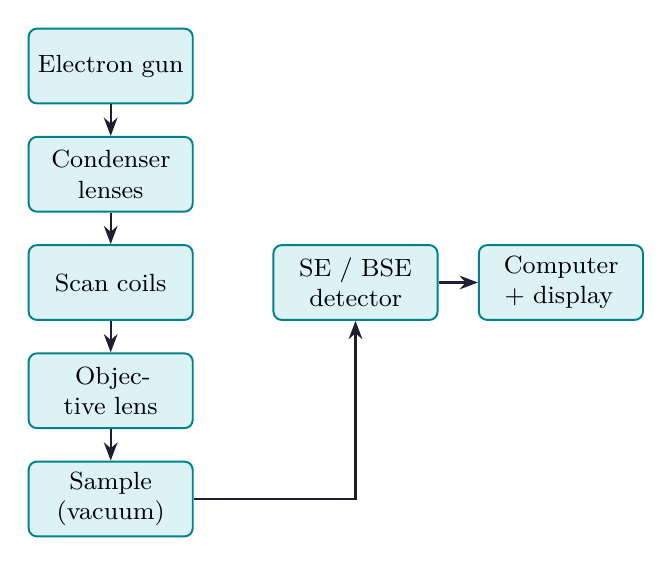
\begin{tikzpicture}[node distance=0.3cm and 0.45cm,
  sblock/.style={rectangle, draw=myteal, fill=hdrteal, text width=1.85cm,
    align=center, minimum height=0.95cm, font=\small,
    rounded corners=3pt, line width=0.7pt}]
  \node[sblock] (n1) {Electron gun};
  \node[sblock, below=0.4cm of n1] (n2) {Condenser lenses};
  \node[sblock, below=0.4cm of n2] (n3) {Scan coils};
  \node[sblock, below=0.4cm of n3] (n4) {Objective lens};
  \node[sblock, below=0.4cm of n4] (n5) {Sample (vacuum)};
  \node[sblock, right=1.0cm of n3] (n6) {SE / BSE detector};
  \node[sblock, right=0.5cm of n6] (n7) {Computer + display};
  \draw[arrow] (n1) -- (n2);
  \draw[arrow] (n2) -- (n3);
  \draw[arrow] (n3) -- (n4);
  \draw[arrow] (n4) -- (n5);
  \draw[arrow] (n5.east) -| (n6.south);
  \draw[arrow] (n6) -- (n7);
\end{tikzpicture}
\end{tcolorbox}

\textbf{Key features of SEM:} resolution $\sim 1\ \mathrm{nm}$, depth of field very large (3D-looking images), needs conducting or coated sample, high vacuum.

\subsection{X-ray Photoelectron Spectroscopy (XPS / ESCA)}
A sample is irradiated with monochromatic soft X-rays (Al~K$\alpha$, $h\nu=1486.6\ \mathrm{eV}$). Core-level electrons are ejected; their kinetic energy is measured.

\begin{tcolorbox}[formulabox, title={XPS Energy-Conservation Equation}]
\[
E_{B}=h\nu - E_{K} - \phi
\]
$E_B$ = binding energy; $E_K$ = kinetic energy of detected photo-electron; $\phi$ = spectrometer work function.\\
$E_B$ is element-specific and shifts with chemical state, e.g.\ Fe(0) vs Fe$_2$O$_3$.
\end{tcolorbox}

\textbf{Information obtained from XPS:}
\begin{itemize}[leftmargin=*, itemsep=1pt, topsep=2pt]
  \item Elemental identification (all elements except H, He).
  \item Oxidation state and chemical environment (chemical shift).
  \item Quantitative composition of top $5$--$10\ \mathrm{nm}$.
  \item Depth profiling when combined with Ar$^{+}$ sputtering.
\end{itemize}

\subsection{Atomic Force Microscopy (AFM)}
A nanometric tip on a flexible cantilever is scanned over the surface. A laser reflected off the cantilever measures sub-nanometre deflections that map height (topography) and tip--surface forces.

\begin{tcolorbox}[tikzbox, title={Working Principle of AFM}]
\centering
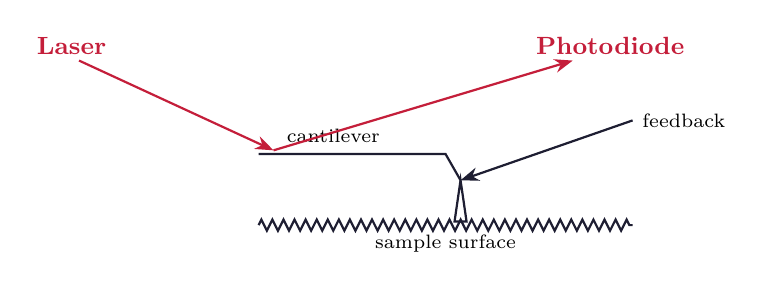
\begin{tikzpicture}[scale=0.95]
  % laser source
  \node[font=\small\bfseries, color=myred] at (0.5,3.4) {Laser};
  \draw[redarrow] (0.6,3.2) -- (3.2,2.0);
  % cantilever
  \draw[thick, mydark] (3.0,1.95) -- (5.5,1.95) -- (5.7,1.6);
  \node[font=\scriptsize] at (4.0,2.2) {cantilever};
  % tip
  \draw[thick, mydark] (5.7,1.6) -- (5.78,1.05) -- (5.62,1.05) -- cycle;
  % sample surface (rough)
  \draw[thick, mydark, decorate, decoration={zigzag, segment length=4pt, amplitude=2pt}]
        (3.0,1.0) -- (8.0,1.0);
  \node[font=\scriptsize] at (5.5,0.75) {sample surface};
  % reflected laser to detector
  \draw[redarrow] (3.2,2.0) -- (7.2,3.2);
  \node[font=\small\bfseries, color=myred] at (7.7,3.4) {Photodiode};
  % feedback
  \node[font=\scriptsize, anchor=west] at (8.0,2.4) {feedback};
  \draw[arrow] (8.0,2.4) -- (5.7,1.6);
\end{tikzpicture}
\end{tcolorbox}

\textbf{Modes of AFM:}
\begin{itemize}[leftmargin=*, itemsep=1pt, topsep=2pt]
  \item \emph{Contact mode}: tip drags on surface; high resolution but can damage soft samples.
  \item \emph{Tapping mode}: cantilever oscillates near resonance, tip touches lightly; safe for biology and polymers.
  \item \emph{Non-contact mode}: tip senses long-range forces; lowest damage.
\end{itemize}

\textbf{Advantages of AFM:} works in air, liquid, and vacuum; no special coating; gives true 3D height; image biological molecules (DNA, proteins) directly.

\subsection{Comparison of Major Surface Techniques}
\begin{tabularx}{\linewidth}{|B{2.4cm}|Y|Y|Y|}
\hline
\textbf{Feature} & \textbf{SEM} & \textbf{AFM} & \textbf{XPS} \\
\hline
Probe & Electrons & Mechanical tip & Soft X-rays \\
\hline
Signal & SE / BSE & Force / deflection & Photo-electrons \\
\hline
Lateral resolution & $\sim 1\ \mathrm{nm}$ & $\sim 0.1\ \mathrm{nm}$ (atomic) & $\sim 10\ \mu\mathrm{m}$ (small spot $\sim 10\ \mu\mathrm{m}$) \\
\hline
Depth probed & Few nm (SE) & Top atomic layer & 5--10 nm \\
\hline
Vacuum & High vacuum & Air / liquid OK & Ultra-high vacuum \\
\hline
Sample preparation & Coat if non-conductive & Almost none & Conductive desirable \\
\hline
Composition info & Possible with EDX & No (height only) & Yes, with chemical state \\
\hline
\end{tabularx}

\subsection{TEM vs SEM}
The two electron-beam microscopies are complementary: SEM gives surface topography while TEM gives internal structure with atomic resolution.

\begin{tabularx}{\linewidth}{|B{2.4cm}|Y|Y|}
\hline
\textbf{Feature} & \textbf{SEM} & \textbf{TEM} \\
\hline
Beam energy & $5$--$30\ \mathrm{kV}$ & $100$--$300\ \mathrm{kV}$ \\
\hline
What is detected & Secondary / back-scattered electrons \emph{above} sample & Electrons \emph{transmitted through} thin sample \\
\hline
Sample form & Bulk, polished, conductive coating if needed & Ultra-thin film ($<100\ \mathrm{nm}$) on grid \\
\hline
Resolution & $\sim 1\ \mathrm{nm}$ & $0.1$--$0.2\ \mathrm{nm}$ (atomic in HRTEM) \\
\hline
Image gives & Topography, depth of field, morphology & Internal structure, lattice fringes, defects \\
\hline
Diffraction option & Limited (EBSD) & Selected-area electron diffraction (SAED) \\
\hline
\end{tabularx}

\subsection{Scanning Tunnelling Microscopy (STM)}
STM achieves true atomic resolution on conducting surfaces by exploiting the quantum tunnelling current that flows between a sharp metal tip and the surface when separated by $\sim 1\ \mathrm{nm}$.

\begin{tcolorbox}[formulabox, title={Tunnelling Current in STM}]
\[
I_{T} \propto V\,\exp(-2\kappa d), \qquad \kappa=\sqrt{\frac{2m_e\phi}{\hbar^{2}}}
\]
$V$ = bias voltage; $d$ = tip--surface gap; $\phi$ = work function. Because $I_T$ falls off exponentially with $d$, a $0.1\ \mathrm{nm}$ change in $d$ changes $I_T$ by a factor of $\sim 10$ — that is the source of atomic-scale sensitivity.
\end{tcolorbox}

\textbf{STM operating modes:}
\begin{itemize}[leftmargin=*, itemsep=1pt, topsep=2pt]
  \item Constant-current mode: feedback adjusts $z$ to keep $I_T$ fixed; image is the $z(x,y)$ map.
  \item Constant-height mode: tip $z$ is fixed; image is the $I_T(x,y)$ map; faster but only safe on flat samples.
\end{itemize}

\textbf{Limitation:} STM only works on conductors and semiconductors, while AFM works on insulators too. STM is the original ``atomic resolution'' technique that won Binnig and Rohrer the 1986 Nobel Prize.

\subsection{BET Surface Area Analysis}
The Brunauer--Emmett--Teller (BET) isotherm extends the Langmuir model to multilayer adsorption and lets you compute the specific surface area of a porous solid from $\mathrm{N_2}$ adsorption at $77\ \mathrm{K}$.

\begin{tcolorbox}[formulabox, title={BET Equation}]
\[
\frac{P/P_0}{V(1-P/P_0)} = \frac{1}{V_m C} + \frac{C-1}{V_m C}\!\left(\frac{P}{P_0}\right)
\]
$P/P_0$ = relative pressure; $V$ = adsorbed volume at $P/P_0$; $V_m$ = monolayer volume; $C$ = BET constant.\\
A plot of LHS vs $P/P_0$ is linear in the range $0.05$--$0.30$. From the slope and intercept, $V_m$ is obtained, and the specific surface area is
\[
S_{\mathrm{BET}} = \frac{V_m\,N_A\,a_m}{V_{\mathrm{molar}}}
\]
where $a_m\approx 0.162\ \mathrm{nm^{2}}$ is the cross-sectional area of an $\mathrm{N_2}$ molecule.
\end{tcolorbox}

\textbf{Why important:} BET surface area is the standard metric for catalysts (Pt/$\gamma$-$\mathrm{Al_2O_3}$ \\$\sim 200\ \mathrm{m^{2}/g}$), zeolites ($\sim 600\ \mathrm{m^{2}/g}$), activated carbon ($>1000\ \mathrm{m^{2}/g}$), and metal-organic frameworks (up to $7000\ \mathrm{m^{2}/g}$).

\subsection{Contact-Angle Measurement: Surface Wettability}
A drop of water on a clean surface forms a contact angle $\theta$ with the surface. This single number is a powerful surface characterisation tool.

\begin{tcolorbox}[formulabox, title={Young's Equation}]
\[
\gamma_{SV}=\gamma_{SL}+\gamma_{LV}\cos\theta
\]
$\gamma_{SV}, \gamma_{SL}, \gamma_{LV}$ = solid--vapour, solid--liquid, liquid--vapour interfacial tensions.\\
\textbf{Hydrophilic} surface: $\theta<90^\circ$ (water spreads). \textbf{Hydrophobic} surface: $\theta>90^\circ$ (water beads). \textbf{Superhydrophobic} (lotus leaf): $\theta>150^\circ$.
\end{tcolorbox}

\textbf{Applications:} surface treatment of biomaterials, anti-fouling coatings, microfluidic device design, paint-adhesion checks.

\begin{tcolorbox}[exambox, title={Exam Points (Section 6)}]
\begin{itemize}[leftmargin=*, itemsep=2pt, topsep=2pt]
  \item Distinguish surface from bulk techniques and explain why probe penetration matters.
  \item For SEM: mention gun, lenses, scan coils, SE/BSE detectors, vacuum.
  \item Quote the XPS equation $E_B=h\nu-E_K-\phi$ and one application (oxidation state).
  \item Sketch AFM tip + cantilever + laser + photodiode.
  \item TEM gives internal structure ($0.1\ \mathrm{nm}$); SEM gives surface topography ($1\ \mathrm{nm}$).
  \item STM tunnelling current $I_T \propto \exp(-2\kappa d)$; works only on conductors.
  \item BET surface area uses $\mathrm{N_2}$ adsorption at $77\ \mathrm{K}$; activated carbon $> 1000\ \mathrm{m^{2}/g}$.
  \item Contact angle: $<90^\circ$ hydrophilic, $>90^\circ$ hydrophobic, $>150^\circ$ superhydrophobic.
\end{itemize}
\end{tcolorbox}

% ===============================================================================
\section{Diffraction and Scattering}
% ===============================================================================

\begin{tcolorbox}[defbox]
\textbf{Diffraction} is the constructive interference of waves scattered by a regular array of atoms or molecules. It produces sharp peaks and is the principal tool for determining crystal structure. \textbf{Scattering} more generally is the redirection of radiation by particles, with or without change of energy; it gives information about size, shape and electron distribution of the scatterers.
\end{tcolorbox}

\subsection{Bragg's Law of X-ray Diffraction}
A crystal acts like a 3D grating because atoms lie on parallel planes separated by an interplanar spacing $d$. Constructive interference occurs at angles satisfying Bragg's law.

\begin{tcolorbox}[formulabox, title={Bragg's Law}]
\[
n\lambda = 2d\sin\theta
\]
$n$ = order (integer); $\lambda$ = wavelength of X-ray (typically Cu~K$\alpha$, $1.5418\,\text{\AA}$); $d$ = interplanar spacing; $\theta$ = Bragg angle (half of the diffraction angle $2\theta$).
\end{tcolorbox}

\begin{tcolorbox}[tikzbox, title={Bragg Reflection from Two Lattice Planes}]
\centering
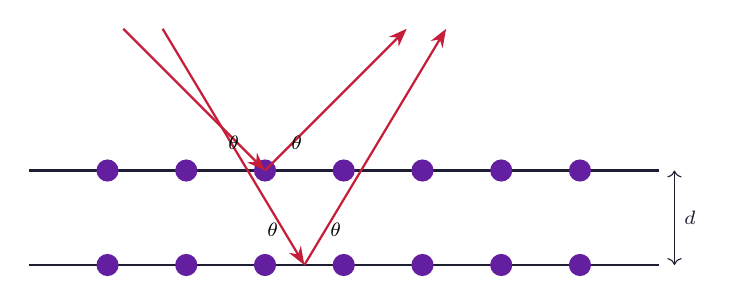
\begin{tikzpicture}[scale=1.0]
  % atomic planes
  \draw[thick, mydark] (0,0) -- (8.0,0);
  \draw[thick, mydark] (0,1.2) -- (8.0,1.2);
  \foreach \x in {1,2,3,4,5,6,7} \fill[mypurple] (\x,0) circle (4pt);
  \foreach \x in {1,2,3,4,5,6,7} \fill[mypurple] (\x,1.2) circle (4pt);
  % d label
  \draw[<->, mydark] (8.2,0) -- (8.2,1.2) node[midway, right, font=\scriptsize] {$d$};
  % incoming/outgoing rays
  \draw[redarrow] (1.2,3.0) -- (3.0,1.2);
  \draw[redarrow] (3.0,1.2) -- (4.8,3.0);
  \draw[redarrow] (1.7,3.0) -- (3.5,0.0);
  \draw[redarrow] (3.5,0.0) -- (5.3,3.0);
  % theta arcs / labels
  \node[font=\scriptsize] at (2.6,1.55) {$\theta$};
  \node[font=\scriptsize] at (3.4,1.55) {$\theta$};
  \node[font=\scriptsize] at (3.1,0.45) {$\theta$};
  \node[font=\scriptsize] at (3.9,0.45) {$\theta$};
\end{tikzpicture}
\end{tcolorbox}

\textbf{Path difference:} The lower ray travels an extra $2d\sin\theta$. Constructive interference (bright spot) requires this to equal $n\lambda$.

\begin{tcolorbox}[examplebox, title={Solved Example: Spacing of NaCl from Bragg Reflection}]
\textbf{Problem:} A first-order ($n=1$) Bragg reflection from NaCl is observed at $\theta=15.5^{\circ}$ with Cu~K$\alpha$ X-rays ($\lambda=0.154\ \mathrm{nm}$). Find the interplanar spacing.

\textbf{Solution:}
\[
d=\frac{n\lambda}{2\sin\theta}=\frac{1\times 0.154}{2\times \sin 15.5^{\circ}}=\frac{0.154}{2\times 0.2672}=0.288\ \mathrm{nm}
\]
This corresponds to the $(200)$ planes of NaCl.
\end{tcolorbox}

\subsection{Powder X-ray Diffraction (PXRD)}
A polycrystalline powder presents all crystallographic orientations to the beam. Each $\{hkl\}$ plane satisfying Bragg's law produces a cone of diffracted intensity, recorded as a series of peaks vs $2\theta$.

\textbf{Information from a powder pattern:}
\begin{itemize}[leftmargin=*, itemsep=1pt, topsep=2pt]
  \item Identification of phases (matched against the ICDD database).
  \item Lattice parameters from peak positions.
  \item Crystallite size from peak broadening (Scherrer formula).
  \item Quantitative phase analysis (Rietveld refinement).
\end{itemize}

\begin{tcolorbox}[formulabox, title={Scherrer Equation for Crystallite Size}]
\[
D=\frac{K\lambda}{\beta\cos\theta}
\]
$D$ = average crystallite size; $K\approx 0.9$ (shape factor); $\beta$ = full-width at half-maximum (FWHM) in radians; $\theta$ = Bragg angle.
\end{tcolorbox}

\subsection{Block Diagram of an X-ray Diffractometer}
\begin{tcolorbox}[tikzbox, title={Block Diagram of a Powder Diffractometer}]
\centering
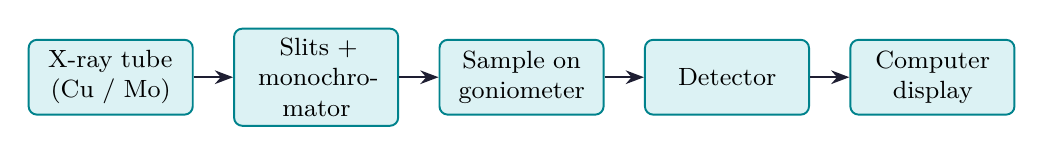
\begin{tikzpicture}[node distance=0.3cm and 0.45cm,
  sblock/.style={rectangle, draw=myteal, fill=hdrteal, text width=1.85cm,
    align=center, minimum height=0.95cm, font=\small,
    rounded corners=3pt, line width=0.7pt}]
  \node[sblock] (n1) {X-ray tube\\(Cu / Mo)};
  \node[sblock, right=0.5cm of n1] (n2) {Slits +\\monochromator};
  \node[sblock, right=0.5cm of n2] (n3) {Sample on goniometer};
  \node[sblock, right=0.5cm of n3] (n4) {Detector};
  \node[sblock, right=0.5cm of n4] (n5) {Computer\\display};
  \draw[arrow] (n1)--(n2);
  \draw[arrow] (n2)--(n3);
  \draw[arrow] (n3)--(n4);
  \draw[arrow] (n4)--(n5);
\end{tikzpicture}
\end{tcolorbox}

\subsection{Electron and Neutron Diffraction}
\begin{tabularx}{\linewidth}{|B{2.4cm}|Y|Y|}
\hline
\textbf{Probe} & \textbf{Wavelength} & \textbf{Speciality} \\
\hline
X-ray & $0.05$--$0.3\ \mathrm{nm}$ & Senses electron density; routine crystallography. \\
\hline
Electron & $\sim 0.005\ \mathrm{nm}$ at 100 kV & Strongly absorbed; ideal for thin films and TEM. \\
\hline
Neutron & $0.1$--$0.3\ \mathrm{nm}$ & Senses nuclear positions, locates light atoms (H, Li); resolves magnetic structure. \\
\hline
\end{tabularx}

\subsection{Rayleigh and Raman Scattering}
When light passes through a transparent medium, a small fraction is scattered. Most of the scattered photons retain the original frequency (\emph{Rayleigh}, elastic). A tiny fraction exchanges energy with molecular vibrations (\emph{Raman}, inelastic).

\begin{tcolorbox}[tikzbox, title={Rayleigh, Stokes and Anti-Stokes Lines in Raman}]
\centering
\begin{tikzpicture}[scale=0.95]
  \draw[->, thick] (0,0) -- (10.4,0) node[right, font=\small] {$\bar{\nu}$};
  \draw[thick, myteal] (5.0,0) -- (5.0,2.4); \node[font=\scriptsize, color=myteal] at (5.0,2.7) {Rayleigh};
  \draw[thick, myred]  (3.4,0) -- (3.4,1.4); \node[font=\scriptsize, color=myred]  at (3.4,1.6) {Stokes};
  \draw[thick, myred]  (6.6,0) -- (6.6,0.7); \node[font=\scriptsize, color=myred]  at (6.6,0.9) {anti-Stokes};
  \draw[<->, dashed, mydark] (5.0,-0.5) -- (3.4,-0.5);
  \node[font=\scriptsize] at (4.2,-0.85) {$+\bar{\nu}_{\text{vib}}$};
  \draw[<->, dashed, mydark] (5.0,-0.5) -- (6.6,-0.5);
  \node[font=\scriptsize] at (5.8,-0.85) {$-\bar{\nu}_{\text{vib}}$};
\end{tikzpicture}
\end{tcolorbox}

\textbf{Raman selection rule:} the vibration must change the molecular polarisability. Combined with the IR rule (dipole change), Raman and IR are often \emph{complementary}.

\begin{tcolorbox}[formulabox, title={Rayleigh Intensity Dependence}]
\[
I_{\mathrm{scat}}\propto \frac{1}{\lambda^{4}}
\]
This $\lambda^{-4}$ dependence explains why the sky is blue (short wavelengths scatter more) and why sunsets are red.
\end{tcolorbox}

\subsection{Other Scattering Techniques}
\begin{tabularx}{\linewidth}{|B{3.0cm}|Y|}
\hline
\textbf{Technique} & \textbf{Information} \\
\hline
Small-angle X-ray scattering (SAXS) & Particle size, shape, $1$--$100\ \mathrm{nm}$ aggregates, polymers. \\
\hline
Dynamic light scattering (DLS) & Hydrodynamic radius and diffusion of nanoparticles in solution. \\
\hline
Static light scattering (SLS) & Molar mass and radius of gyration of polymers (Zimm plot). \\
\hline
Surface-enhanced Raman (SERS) & Trace molecule detection on rough Ag/Au surfaces; single-molecule sensitivity. \\
\hline
\end{tabularx}

\subsection{Applications of Diffraction and Scattering}
\begin{itemize}[leftmargin=*, itemsep=2pt, topsep=2pt]
  \item Crystal-structure determination of metals, ceramics, drugs and proteins.
  \item Phase identification in alloys and minerals.
  \item Quality control of pharmaceuticals (polymorphs).
  \item Thin-film analysis (texture, residual stress) by glancing-incidence XRD.
  \item Particle-size and aggregation studies (DLS, SAXS).
  \item Vibrational fingerprinting using Raman; complements IR.
\end{itemize}

\subsection{Three Classical X-ray Diffraction Methods}
There are three historical setups, each suited to a different sample form.

\begin{tabularx}{\linewidth}{|B{2.6cm}|Y|Y|}
\hline
\textbf{Method} & \textbf{Sample} & \textbf{What is varied} \\
\hline
Laue method & Single crystal, fixed orientation & Polychromatic X-rays (white beam); each plane satisfies Bragg at its own $\lambda$. Used to find crystal symmetry and orient single crystals. \\
\hline
Rotating-crystal method & Single crystal mounted on a goniometer & Crystal rotated; monochromatic $\lambda$. Records reflections from all planes during rotation. \\
\hline
Debye--Scherrer (powder) method & Polycrystalline powder & Random orientations present every plane to the beam; monochromatic $\lambda$. Produces concentric cones, recorded as a $2\theta$ pattern. Most common in materials labs. \\
\hline
\end{tabularx}

\subsection{Raman Effect: Quantum Picture}
Stokes and anti-Stokes lines arise because the molecule can either gain (anti-Stokes) or lose (Stokes) one vibrational quantum during the inelastic scattering event.

\begin{tcolorbox}[formulabox, title={Stokes / Anti-Stokes Intensity Ratio}]
\[
\frac{I_{\text{anti-Stokes}}}{I_{\text{Stokes}}} = \!\left(\frac{\bar{\nu}_0+\bar{\nu}_v}{\bar{\nu}_0-\bar{\nu}_v}\right)^{\!4}\exp\!\left(-\frac{hc\,\bar{\nu}_v}{k_B T}\right)
\]
At room temperature anti-Stokes lines are much weaker because few molecules occupy the $v=1$ state. Heating the sample increases the anti-Stokes/Stokes ratio --- an old way to measure local temperature.
\end{tcolorbox}

\subsection{Why the Sky is Blue: A Worked Rayleigh Calculation}
Sunlight contains all visible wavelengths. Each colour scatters with intensity $\propto 1/\lambda^{4}$.

\begin{tcolorbox}[examplebox, title={Solved Example: Blue / Red Scattering Ratio}]
\textbf{Problem:} Compare the Rayleigh-scattered intensity of blue ($\lambda=470\ \mathrm{nm}$) and red ($\lambda=650\ \mathrm{nm}$) light.

\textbf{Solution:}
\[
\frac{I_{\mathrm{blue}}}{I_{\mathrm{red}}}=\!\left(\frac{650}{470}\right)^{\!4}=(1.383)^{4}=3.66
\]
Blue light is scattered $\sim 3.7\times$ more strongly than red. When you look up away from the sun, you see this scattered blue light; when you look directly at sunset/sunrise the direct beam has been depleted of blue and appears red.
\end{tcolorbox}

\subsection{Raman Spectroscopy: Practical Applications}
Beyond the engineering chemistry textbook, Raman is now a workhorse technique in industry and forensics.

\begin{itemize}[leftmargin=*, itemsep=1pt, topsep=2pt]
  \item Pharmaceutical quality control: through-bottle identification of API and excipients (TRS technology).
  \item Polymorph screening in drug formulation.
  \item Forensic analysis of paints, fibres, narcotics --- non-destructive, no sample prep.
  \item Identification of pigments in art and archaeology (no sampling of priceless objects).
  \item Carbon-material characterisation: D, G and 2D bands in graphene/CNT.
  \item Biomedical Raman: in-vivo cancer margin detection (handheld probes).
  \item SERS for trace explosives and pesticide residue detection.
\end{itemize}

\begin{tcolorbox}[masonbox, title={IR vs Raman: Complementary Spectra of \texorpdfstring{$\mathrm{CO_2}$}{CO2}}]
$\mathrm{CO_2}$ has four vibrational modes. The symmetric stretch is Raman-active (IR-inactive), while the asymmetric stretch and the two bends are IR-active (Raman-inactive). Together IR + Raman map all modes — a direct application of the mutual exclusion principle.
\end{tcolorbox}

\begin{tcolorbox}[exambox, title={Exam Points (Section 7)}]
\begin{itemize}[leftmargin=*, itemsep=2pt, topsep=2pt]
  \item Always state Bragg's law with all symbols defined.
  \item Mention the use of Cu~K$\alpha$ ($\lambda=1.54\,\text{\AA}$) and that we measure peak position $2\theta$.
  \item For nanoparticles, recall Scherrer's equation $D=K\lambda/(\beta\cos\theta)$.
  \item Distinguish Rayleigh (elastic) vs Raman (inelastic) and link to selection rules.
  \item Quote the $1/\lambda^{4}$ Rayleigh law and ``why the sky is blue''.
  \item Three classical XRD methods: Laue (single crystal, polychromatic), rotating-crystal, Debye--Scherrer (powder).
  \item Anti-Stokes/Stokes intensity ratio depends on temperature --- thermometry application.
  \item SERS gives single-molecule sensitivity for forensic and trace detection.
\end{itemize}
\end{tcolorbox}

\newpage
\begin{center}
  {\large\bfseries\color{myred} Quick Revision --- Module 2}\\[3pt]
  {\small\color{mydark} Spectroscopic Techniques and Applications $|$ BS-CH101}
\end{center}
\noindent{\color{myred}\rule{\linewidth}{1.2pt}}
\vspace{4pt}

\begin{tcolorbox}[formulabox, breakable, title={Key Formulas at a Glance},
  title after break={\textbf{Key Formulas at a Glance (contd.)}}]
\begin{tabularx}{\linewidth}{|B{4.4cm}|Y|}
\hline
\textbf{Formula / Rule} & \textbf{Meaning} \\
\hline
$E=h\nu=\displaystyle\frac{hc}{\lambda}=hc\bar{\nu}$ & Photon energy in terms of $\nu, \lambda, \bar{\nu}$. \\
\hline
$\Delta E=h\nu$ & Bohr resonance condition for absorption / emission. \\
\hline
$P_{1\to 2}\propto |\mu_{12}|^{2}$ & Transition probability; selection rules emerge here. \\
\hline
$\dfrac{N_2}{N_1}=\dfrac{g_2}{g_1}\,e^{-\Delta E/k_B T}$ & Boltzmann level population. \\
\hline
$A=\varepsilon c l$ & Beer--Lambert law for UV-Vis quantitation. \\
\hline
$\Phi_F=\dfrac{k_F}{k_F+k_{NR}+k_{ISC}}$ & Fluorescence quantum yield. \\
\hline
$\dfrac{F_0}{F}=1+K_{SV}[Q]$ & Stern--Volmer quenching. \\
\hline
$\bar{B}=\dfrac{h}{8\pi^{2}cI}$, $\,I=\mu r^{2}$ & Rotational constant and moment of inertia. \\
\hline
$E_v=(v+\tfrac12)h\nu_0$ & Harmonic-oscillator vibrational energy. \\
\hline
$\bar{\nu}_0=\dfrac{1}{2\pi c}\sqrt{\dfrac{k}{\mu}}$ & Vibrational wavenumber. \\
\hline
$\nu_L=\dfrac{\gamma B_0}{2\pi}$ & NMR Larmor (resonance) frequency. \\
\hline
$\delta\,(\mathrm{ppm})=\dfrac{\nu_{\text{sample}}-\nu_{\text{TMS}}}{\nu_{\text{spec}}}\times 10^{6}$ & NMR chemical shift relative to TMS. \\
\hline
\end{tabularx}
\vspace{3pt}
\begin{tabularx}{\linewidth}{|B{4.4cm}|Y|}
\hline
$E_B=h\nu-E_K-\phi$ & XPS binding-energy equation. \\
\hline
$n\lambda=2d\sin\theta$ & Bragg's law for X-ray diffraction. \\
\hline
$D=\dfrac{K\lambda}{\beta\cos\theta}$ & Scherrer equation, crystallite size. \\
\hline
$I_{\text{scat}}\propto 1/\lambda^{4}$ & Rayleigh scattering law. \\
\hline
$\lambda_{\max} = \lambda_{\mathrm{base}} + \sum \text{increments}$ & Woodward--Fieser empirical prediction. \\
\hline
$E = \displaystyle\frac{R_0^{6}}{R_0^{6}+r^{6}}$ & FRET efficiency. \\
\hline
$\displaystyle\frac{\bar{\nu}_{\mathrm{D}}}{\bar{\nu}_{\mathrm{H}}} = \sqrt{\mu_{\mathrm{H}}/\mu_{\mathrm{D}}}$ & Isotope shift ($\approx 1/\sqrt{2}$ for X--H/X--D). \\
\hline
$\Phi_F = k_F\,\tau_F$ & Quantum-yield/lifetime relation. \\
\hline
$\displaystyle\frac{A_{21}}{B_{21}}=\frac{8\pi h\nu^{3}}{c^{3}}$ & Einstein A/B coefficient ratio. \\
\hline
$I_T \propto \exp(-2\kappa d)$ & STM tunnelling current (atomic resolution). \\
\hline
$\gamma_{SV}=\gamma_{SL}+\gamma_{LV}\cos\theta$ & Young's equation for contact angle. \\
\hline
$S_{\mathrm{BET}}=\displaystyle\frac{V_m N_A a_m}{V_{\mathrm{molar}}}$ & BET specific surface area. \\
\hline
\end{tabularx}
\end{tcolorbox}

\begin{tcolorbox}[defbox, title={One-Line Definitions}]
\begin{itemize}[leftmargin=*, itemsep=2pt, topsep=2pt]
  \item \textbf{Spectroscopy:} Study of interaction of EM radiation with matter.
  \item \textbf{Selection rule:} Quantum-number condition that decides whether a transition is allowed.
  \item \textbf{Chromophore:} Functional group responsible for absorption of UV-Vis light.
  \item \textbf{Auxochrome:} Saturated group that shifts and intensifies an existing chromophore.
  \item \textbf{Bathochromic shift:} Movement of $\lambda_{\max}$ to longer wavelength (red shift).
  \item \textbf{Fluorescence:} Spin-allowed radiative emission from $S_1$ to $S_0$.
  \item \textbf{Phosphorescence:} Radiative $T_1\to S_0$ emission, long-lived afterglow.
  \item \textbf{Stokes shift:} Difference between absorption and emission maxima.
  \item \textbf{Quantum yield ($\Phi_F$):} Fraction of absorbed photons re-emitted as fluorescence.
  \item \textbf{Rotational constant ($\bar{B}$):} Inverse moment of inertia in $\mathrm{cm^{-1}}$.
  \item \textbf{Reduced mass ($\mu$):} $m_1 m_2/(m_1+m_2)$ for a diatomic molecule.
  \item \textbf{Force constant ($k$):} Stiffness of a bond modelled as a spring.
  \item \textbf{Chemical shift ($\delta$):} NMR resonance position relative to TMS, in ppm.
  \item \textbf{Larmor frequency:} Resonance $\nu$ of a nuclear spin in a field $B_0$.
  \item \textbf{MRI gradient:} Linear field variation that encodes spatial position.
  \item \textbf{Bragg angle:} Half of the diffraction angle at which constructive interference occurs.
  \item \textbf{Crystallite size (Scherrer):} Average coherent domain size estimated from peak broadening.
  \item \textbf{Rayleigh scattering:} Elastic redirection of light by sub-wavelength particles.
  \item \textbf{Raman scattering:} Inelastic scattering with vibrational energy exchange.
  \item \textbf{Mutual exclusion principle:} For molecules with a centre of symmetry, IR-active modes are Raman-inactive and vice-versa.
  \item \textbf{Franck--Condon principle:} Electronic transitions are vertical because nuclei do not move on the timescale of electronic excitation.
  \item \textbf{Einstein coefficients:} Three rate constants $A_{21}, B_{12}, B_{21}$ describing spontaneous emission, stimulated absorption and stimulated emission.
  \item \textbf{Kasha's rule:} Emission always originates from the lowest excited state of a given multiplicity.
  \item \textbf{FRET:} Distance-dependent non-radiative dipole--dipole energy transfer; $E\propto 1/r^{6}$.
  \item \textbf{Woodward--Fieser rules:} Empirical formula to predict $\lambda_{\max}$ of dienes and enones.
  \item \textbf{Isosbestic point:} Wavelength where two interconverting species have equal $\varepsilon$.
  \item \textbf{Coupling constant ($J$):} Spacing within a multiplet in Hz; independent of $B_0$.
  \item \textbf{Integration:} Area under an NMR signal, proportional to the number of equivalent protons.
  \item \textbf{Ring-current effect:} Aromatic $\pi$-electron circulation deshields ring protons.
  \item \textbf{Gd-DTPA:} Gadolinium chelate used as $T_1$-shortening MRI contrast agent.
  \item \textbf{BET surface area:} Specific surface area measured by $\mathrm{N_2}$ adsorption at $77\ \mathrm{K}$.
  \item \textbf{STM:} Atomic-resolution microscopy based on quantum tunnelling current between tip and conducting surface.
  \item \textbf{Contact angle:} Angle a liquid drop makes with a solid surface; quantifies wettability.
  \item \textbf{Laue method:} Single-crystal XRD with a polychromatic beam, used to determine crystal orientation.
\end{itemize}
\end{tcolorbox}

\begin{tcolorbox}[exambox, title={Frequently Asked / Viva Questions}]
\begin{enumerate}[topsep=0pt, label=\textbf{Q\arabic*.}, itemsep=5pt]
  \item \Q{State the principle of spectroscopy.}
    A molecule absorbs a photon when its energy matches the gap between two allowed levels: $\Delta E = h\nu$.
  \item \Q{What are gross and specific selection rules?}
    Gross rule sets a property the molecule must have (dipole, polarisability, spin), specific rule restricts the change in quantum numbers (e.g.\ $\Delta v=\pm 1$).
  \item \Q{Why is $\mathrm{N_2}$ IR-inactive but Raman-active?}
    The $\mathrm{N_2}$ stretch does not change the dipole moment (zero) but does change polarisability.
  \item \Q{State Beer--Lambert law and one limitation.}
    $A=\varepsilon c l$. It fails at high concentration because intermolecular interactions alter $\varepsilon$.
  \item \Q{Define chromophore and give two examples.}
    Unsaturated group responsible for UV-Vis absorption; e.g.\ $\mathrm{C{=}O}$, $\mathrm{C{=}C}$.
  \item \Q{What is the difference between fluorescence and phosphorescence?}
    Fluorescence is spin-allowed $S_1\to S_0$ ($10^{-9}$--$10^{-7}\ \mathrm{s}$); phosphorescence is spin-forbidden $T_1\to S_0$ ($10^{-3}$--$10\ \mathrm{s}$).
  \item \Q{Name two medical uses of fluorescence.}
    Fluorescein retinal angiography and photodynamic therapy of cancer.
  \item \Q{Why does $\mathrm{HCl}$ show a microwave spectrum but $\mathrm{H_2}$ does not?}
    Only $\mathrm{HCl}$ has a permanent electric dipole; the rotational gross rule fails for $\mathrm{H_2}$.
  \item \Q{State the harmonic-oscillator selection rule for IR.}
    $\Delta v = \pm 1$, with the requirement that the vibration changes the dipole moment.
  \item \Q{State the Larmor equation.}
    $\nu_L=\gamma B_0/(2\pi)$; for $^{1}\mathrm{H}$ at $11.74\ \mathrm{T}$, $\nu_L=500\ \mathrm{MHz}$.
  \item \Q{What is chemical shift in NMR?}
    Position of a resonance in ppm relative to TMS: $\delta=(\nu_s-\nu_{\mathrm{TMS}})/\nu_{\mathrm{spec}}\times 10^{6}$.
  \item \Q{How does MRI distinguish tissues?}
    Through differences in proton density, $T_1$ and $T_2$ relaxation times of water in each tissue.
  \item \Q{Give two surface techniques and one piece of information each.}
    SEM (topography), XPS (oxidation state of surface atoms).
  \item \Q{State Bragg's law.}
    $n\lambda = 2d\sin\theta$; gives $d$-spacings of crystal planes from peak positions.
  \item \Q{Differentiate Rayleigh and Raman scattering.}
    Rayleigh is elastic, same $\nu$. Raman is inelastic, $\pm \bar{\nu}_{\mathrm{vib}}$ shifted lines.
  \item \Q{State Franck--Condon principle.}
    Electronic transitions are vertical on a potential-energy diagram because nuclei do not move during the $10^{-15}\ \mathrm{s}$ duration of electronic absorption.
  \item \Q{What does Kasha's rule state?}
    Emission almost always originates from the lowest vibrational level of the lowest excited state of a given spin multiplicity, regardless of the excitation wavelength.
  \item \Q{Define FRET and give one application.}
    Non-radiative resonance energy transfer from an excited donor to a nearby acceptor; $E\propto R_0^{6}/(R_0^{6}+r^{6})$. Used as a molecular ruler in single-molecule biophysics and TaqMan PCR.
  \item \Q{State Woodward--Fieser rules.}
    Empirical addition of base value plus increments for substituents predicts $\lambda_{\max}$ of dienes ($215\ \mathrm{nm}$ acyclic) and $\alpha,\beta$-unsaturated ketones ($215\ \mathrm{nm}$ acyclic) within $\pm 5\ \mathrm{nm}$.
  \item \Q{What is an isosbestic point?}
    Wavelength where two interconverting species have equal $\varepsilon$; presence of a sharp isosbestic point confirms a clean two-component equilibrium.
  \item \Q{Why does $\mathrm{D{-}Cl}$ absorb at lower wavenumber than $\mathrm{H{-}Cl}$?}
    Same force constant but doubled reduced mass; $\bar{\nu}\propto 1/\sqrt{\mu}$ gives a factor of $\sim 0.71$. So DCl absorbs at $\sim 2137\ \mathrm{cm^{-1}}$ vs HCl at $2989\ \mathrm{cm^{-1}}$.
  \item \Q{What information does NMR integration give?}
    Area under a peak is proportional to the number of equivalent protons in that environment, providing the H-count of each chemical type.
  \item \Q{What is the coupling constant $J$ and how do you measure it?}
    Spacing within a multiplet, expressed in Hz, independent of $B_0$. It is read directly from line spacing in the spectrum and is diagnostic of cis/trans, geminal/vicinal coupling.
  \item \Q{Name two MRI contrast agents.}
    Gd-DTPA (Magnevist) shortens water $T_1$ to brighten tissues; SPIONs shorten $T_2$ to darken regions where they accumulate.
  \item \Q{How does STM achieve atomic resolution?}
    Tunnelling current $I_T\propto \exp(-2\kappa d)$ falls off exponentially with tip--surface gap, so a $0.1\ \mathrm{nm}$ change alters the current by $\sim 10\times$.
  \item \Q{What is BET surface area?}
    Specific surface area of porous solids measured from $\mathrm{N_2}$ adsorption at $77\ \mathrm{K}$ using the BET multilayer-isotherm equation. Activated carbon $>1000\ \mathrm{m^{2}/g}$.
  \item \Q{What is the contact angle and what does it tell you?}
    Angle a sessile drop makes with a surface; $<90^\circ$ hydrophilic, $>90^\circ$ hydrophobic, $>150^\circ$ superhydrophobic. Quantifies surface wettability via Young's equation.
  \item \Q{Why is the sky blue and the sunset red?}
    Rayleigh-scattered intensity $\propto 1/\lambda^{4}$, so blue scatters $\sim 3.7\times$ more than red. Looking up reveals scattered blue; the direct sunset beam has been depleted of blue and looks red.
\end{enumerate}
\end{tcolorbox}

\begin{tcolorbox}[tikzbox, title={Summary Reference Table of Spectroscopic Techniques}]
\begin{tabularx}{\linewidth}{|B{3.0cm}|Y|Y|Y|}
\hline
\textbf{Technique} & \textbf{Region / probe} & \textbf{Information} & \textbf{Key formula / rule} \\
\hline
UV-Vis & 200--800 nm photons & Electronic transitions, concentration & $A=\varepsilon c l$ \\
\hline
Fluorescence & UV-Vis emission & Excited state, medical imaging & $\Phi_F$, Stern--Volmer \\
\hline
IR / FT-IR & $400$--$4000\ \mathrm{cm^{-1}}$ & Functional groups & $\bar{\nu}_0=\frac{1}{2\pi c}\sqrt{k/\mu}$ \\
\hline
Microwave & $1$--$300\ \mathrm{GHz}$ & Bond length, $I$, $\bar{B}$ & $\bar{B}=h/(8\pi^{2}cI)$ \\
\hline
NMR & RF in strong $B_0$ & H/C environments, structure & $\nu_L=\gamma B_0/(2\pi)$ \\
\hline
MRI & RF + magnetic gradients & Soft-tissue images & $T_1, T_2$ contrast \\
\hline
SEM / AFM / XPS & Electrons / tip / X-rays & Surface morphology + chemistry & $E_B=h\nu-E_K-\phi$ (XPS) \\
\hline
XRD & X-rays on crystal & Crystal structure, $d$-spacings & $n\lambda=2d\sin\theta$ \\
\hline
Raman & Vis/NIR scattering & Vibrational + symmetry info & Polarisability change \\
\hline
\end{tabularx}
\end{tcolorbox}

\newpage
% ============================================================================
\renewcommand{\moduletitle}{Module 3 --- Intermolecular Forces}
\part{Module 3: Intermolecular Forces, Real Gases and Critical Phenomena}
\setcounter{section}{0}
% ============================================================================

% ===============================================================================
\section{Intermolecular Forces: Classification and Origin}
% ===============================================================================

\begin{tcolorbox}[defbox]
\textbf{Intermolecular forces (IMF)} are attractive or repulsive forces between molecules, atoms, or ions that are not covalently bonded. They arise from electrostatic interactions between charge distributions and are the cause of condensation, surface tension, viscosity, solubility, and deviation from ideal-gas behaviour. They are \emph{weaker} than intramolecular (covalent/ionic) bonds but collectively determine the physical state and material properties of matter.
\end{tcolorbox}

\subsection{Classification of Intermolecular Forces}
All intermolecular forces can be traced to Coulomb's law: $V \propto q_1 q_2 / r$. Depending on whether the charges are permanent, induced, or fluctuating, we get different categories.

\begin{tabularx}{\linewidth}{|B{2.8cm}|Y|Y|Y|}
\hline
\textbf{Force} & \textbf{Between} & \textbf{Origin} & \textbf{Example} \\
\hline
Ion--ion & Two ions & Full charges $q_1q_2$ & NaCl lattice \\
\hline
Ion--dipole & Ion + polar molecule & Charge + permanent dipole & $\mathrm{Na^+}$--water hydration \\
\hline
Dipole--dipole (Keesom) & Two polar molecules & Two permanent dipoles & HCl--HCl, acetone \\
\hline
Dipole--induced dipole (Debye) & Polar + polarisable molecule & Permanent dipole induces temporary dipole & HCl--Ar \\
\hline
Dispersion (London) & Any two molecules & Instantaneous dipole--induced dipole & Ar--Ar, $\mathrm{CH_4}$ \\
\hline
Hydrogen bonding & H covalently bonded to F, O, N & Electrostatic + partial covalent & Water, HF, DNA \\
\hline
\end{tabularx}

\subsection{Ionic Interactions}
An ionic interaction is the electrostatic attraction between oppositely charged ions. It is the strongest non-covalent force.

\begin{tcolorbox}[formulabox, title={Coulomb Potential Between Two Ions}]
\[
V_{\mathrm{ion-ion}}=-\frac{z_1 z_2 e^2}{4\pi\varepsilon_0 r}
\]
$z_1, z_2$ = signed charge numbers; $e=1.602\times10^{-19}\ \mathrm{C}$; $r$ = interionic distance; $\varepsilon_0=8.854\times10^{-12}\ \mathrm{C^2\,N^{-1}\,m^{-2}}$.\\[2pt]
Energy falls as $1/r$ (long range). In a crystal, many-ion Madelung sums give the lattice energy.
\end{tcolorbox}

\textbf{Lattice energy and Born--Haber cycle:} The Born--Haber cycle uses Hess's law to evaluate the lattice energy $U_L$ indirectly, since direct measurement is impossible:
\[
U_L = \Delta H_f^\circ(\mathrm{salt}) - \Delta H_{\mathrm{sub}} - \Delta H_{\mathrm{IE}} - \tfrac12 \Delta H_{\mathrm{diss}} - \Delta H_{\mathrm{EA}}
\]
Higher lattice energy means harder crystal, higher melting point. $\mathrm{MgO}$ ($U_L\approx3850\ \mathrm{kJ\,mol^{-1}}$) is harder than $\mathrm{NaCl}$ ($U_L\approx787\ \mathrm{kJ\,mol^{-1}}$) because $\mathrm{Mg^{2+}/O^{2-}}$ charges are double.

\subsection{Dipole Moment and Polar Molecules}

\begin{tcolorbox}[defbox]
\textbf{Dipole moment} $\vec{\mu}$ arises whenever positive and negative charge centres do not coincide. For a diatomic $\mathrm{A{-}B}$: $\mu = q\cdot d$, where $q$ is the partial charge and $d$ is the bond length. Units: debye (D), $1\ \mathrm{D}=3.336\times10^{-30}\ \mathrm{C\,m}$.
\end{tcolorbox}

\begin{tabularx}{\linewidth}{|B{2.6cm}|Y|Y|}
\hline
\textbf{Molecule} & \textbf{$\mu$ (D)} & \textbf{Comment} \\
\hline
$\mathrm{H_2O}$ & 1.85 & Bent structure, dipoles add \\
\hline
$\mathrm{NH_3}$ & 1.47 & Pyramidal \\
\hline
$\mathrm{HCl}$ & 1.08 & Heteronuclear diatomic \\
\hline
$\mathrm{CO_2}$ & 0 & Linear, dipoles cancel \\
\hline
$\mathrm{CCl_4}$ & 0 & Tetrahedral, dipoles cancel \\
\hline
$\mathrm{CHCl_3}$ & 1.01 & Asymmetric tetrahedral \\
\hline
\end{tabularx}

\textbf{Why $\mathrm{CO_2}$ and $\mathrm{CCl_4}$ are non-polar:} Each individual bond is polar but the vector sum of all bond dipoles is zero due to the symmetric geometry.

\subsection{Dipole--Dipole (Keesom) Interaction}
Two polar molecules attract when oppositely charged ends face each other and repel when like ends face. After thermal averaging over all orientations:

\begin{tcolorbox}[formulabox, title={Keesom Orientational Energy (Thermal Average)}]
\[
V_{\mathrm{Keesom}} = -\frac{2\mu_1^2\mu_2^2}{3(4\pi\varepsilon_0)^2 k_B T\,r^6}
\]
Key feature: falls as $r^{-6}$ and is temperature-dependent (decreases at higher $T$ because thermal motion disrupts orientation).
\end{tcolorbox}

\subsection{Dipole--Induced Dipole (Debye) Interaction}
A polar molecule distorts the electron cloud of a nearby polarisable, non-polar molecule creating an induced dipole. The interaction is always attractive.

\begin{tcolorbox}[formulabox, title={Debye Induction Energy}]
\[
V_{\mathrm{Debye}} = -\frac{\mu^2\alpha'}{(4\pi\varepsilon_0)^2 r^6}
\]
$\alpha'$ = polarisability volume (SI: $\mathrm{C^2\,m^2\,J^{-1}}$; often tabulated in \r{A}$^3$). Like Keesom, falls as $r^{-6}$ but is \emph{temperature-independent}.
\end{tcolorbox}

\subsection{London Dispersion Forces}
Even completely non-polar atoms/molecules (noble gases, hydrocarbons) attract each other and can be liquefied. This requires a quantum-mechanical explanation.

\begin{tcolorbox}[defbox]
\textbf{London dispersion (induced-dipole--induced-dipole) force:} At any instant, the electron distribution in an atom fluctuates, creating a transient dipole. This instantaneous dipole polarises a neighbouring atom, inducing a correlated dipole. The time-averaged interaction is always \emph{attractive}.
\end{tcolorbox}

\begin{tcolorbox}[formulabox, title={London Dispersion Energy}]
\[
V_{\mathrm{London}} = -\frac{3}{2}\,\frac{\alpha_1'\alpha_2'}{(4\pi\varepsilon_0)^2 r^6}\cdot\frac{I_1 I_2}{I_1+I_2}
\]
$I_1, I_2$ = ionisation energies; $\alpha_1', \alpha_2'$ = polarisability volumes.\\
Key: falls as $\boldsymbol{r^{-6}}$; increases with polarisability (larger molecules, more electrons, heavier atoms).
\end{tcolorbox}

\textbf{Why dispersion forces increase down a group:}

\begin{tabularx}{\linewidth}{|B{2.4cm}|Y|Y|Y|}
\hline
\textbf{Noble gas} & \textbf{Polarisability (pm$^3$)} & \textbf{Boiling point (K)} & \textbf{Trend} \\
\hline
He & 2.3 & 4.2 & \\
\hline
Ne & 4.0 & 27.1 & \\
\hline
Ar & 16.3 & 87.3 & Increasing down \\
\hline
Kr & 24.8 & 119.9 & \\
\hline
Xe & 40.4 & 165.1 & \\
\hline
\end{tabularx}

\begin{tcolorbox}[examplebox, title={Solved Example: Why Hexane Boils at 69$^\circ$C but Pentane at 36$^\circ$C}]
Both are non-polar and rely on London dispersion only. Hexane ($\mathrm{C_6H_{14}}$, MW = 86) has more electrons and higher polarisability than pentane ($\mathrm{C_5H_{12}}$, MW = 72). The stronger London forces require more energy to overcome, raising the boiling point by $\sim33^\circ\mathrm{C}$.
\end{tcolorbox}

\subsection{Hydrogen Bonding}
Hydrogen bonding is the strongest intermolecular interaction between neutral molecules ($15$--$40\ \mathrm{kJ\,mol^{-1}}$, about 10--20\% of a covalent bond). It requires:
\begin{enumerate}[leftmargin=*, itemsep=1pt, topsep=2pt]
  \item A hydrogen covalently bonded to a highly electronegative atom (F, O, or N) --- the \emph{donor}.
  \item A nearby lone pair on another electronegative atom --- the \emph{acceptor}.
\end{enumerate}

\begin{tcolorbox}[tikzbox, title={Hydrogen Bonding in Water}]
\centering
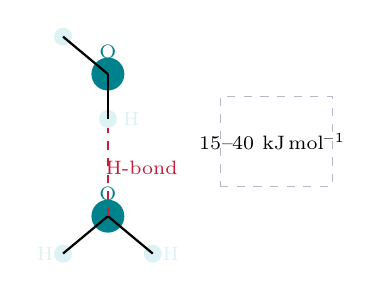
\begin{tikzpicture}[scale=0.95]
  % Molecule 1
  \fill[myteal]   (0,0) circle (0.22) node[above=2pt, font=\scriptsize] {O};
  \fill[hdrteal]  (-0.6,-0.5) circle (0.12) node[left, font=\scriptsize] {H};
  \fill[hdrteal]  (0.6,-0.5) circle (0.12) node[right, font=\scriptsize] {H};
  \draw[thick] (0,0)--(-0.6,-0.5);
  \draw[thick] (0,0)--(0.6,-0.5);
  % H-bond
  \draw[dashed, myred, thick] (0,0)--(0,1.3);
  \node[font=\scriptsize, color=myred] at (0.45,0.65) {H-bond};
  % Molecule 2
  \fill[myteal]   (0,1.9) circle (0.22) node[above=2pt, font=\scriptsize] {O};
  \fill[hdrteal]  (-0.6,2.4) circle (0.12);
  \fill[hdrteal]  (0,1.3)    circle (0.12) node[right=2pt, font=\scriptsize] {H};
  \draw[thick] (0,1.9)--(-0.6,2.4);
  \draw[thick] (0,1.9)--(0,1.3);
  \node[font=\scriptsize] at (2.2,1.0) {$15$--$40\ \mathrm{kJ\,mol^{-1}}$};
  \draw[dashed, mgframe] (1.5,0.4)--(3.0,0.4)--(3.0,1.6)--(1.5,1.6)--cycle;
\end{tikzpicture}
\end{tcolorbox}

\textbf{Consequences of hydrogen bonding:}
\begin{itemize}[leftmargin=*, itemsep=2pt, topsep=2pt]
  \item Anomalously high boiling points: water (100$^\circ$C) vs $\mathrm{H_2S}$ ($-60^\circ$C), HF (19.5$^\circ$C) vs HCl ($-85^\circ$C).
  \item High heat of vaporisation of water ($44\ \mathrm{kJ\,mol^{-1}}$).
  \item Ice is less dense than liquid water (open hydrogen-bonded network).
  \item Protein secondary structure (alpha helix: $i$ to $i+4$ N--H$\cdots$O$=$C).
  \item DNA double helix held by A--T (2 H-bonds) and G--C (3 H-bonds) base pairing.
\end{itemize}

\textbf{Intermolecular vs intramolecular H-bonding:}\par\noindent
\begin{tabularx}{\linewidth}{|B{3.2cm}|Y|Y|}
\hline
\textbf{Type} & \textbf{Occurs between} & \textbf{Effect} \\
\hline
Intermolecular & Different molecules & Higher bp, greater association in solution \\
\hline
Intramolecular & Within same molecule & Lower bp than without H-bond; less association \\
\hline
\end{tabularx}

Example: \emph{ortho}-nitrophenol has an intramolecular H-bond between OH and the adjacent $\mathrm{NO_2}$; \emph{para}-nitrophenol cannot, so it forms intermolecular H-bonds and has a higher melting point.

\subsection{Polarisability and Its Determinants}

\begin{tcolorbox}[defbox]
\textbf{Polarisability} $\alpha$ measures how easily the electron cloud of an atom or molecule is distorted by an external electric field. Induced dipole $\mu_{\mathrm{ind}} = \alpha E$.
\end{tcolorbox}

Polarisability increases with:
\begin{itemize}[leftmargin=*, itemsep=1pt, topsep=2pt]
  \item Increasing number of electrons (larger atoms, heavier atoms down a group).
  \item Larger atomic radius.
  \item $\pi$-electron systems (benzene, graphene).
  \item Ease of electron delocalisation.
\end{itemize}

\subsection{Relative Strengths: Summary Table}
\begin{tabularx}{\linewidth}{|B{2.8cm}|Y|Y|Y|}
\hline
\textbf{Force} & \textbf{Range} & \textbf{Energy (kJ mol$^{-1}$)} & \textbf{$r$ dependence} \\
\hline
Ion--ion & Long & $250$--$1000$ & $r^{-1}$ \\
\hline
Ion--dipole & Medium & $15$--$85$ & $r^{-2}$ \\
\hline
H-bond & Short--medium & $15$--$40$ & $r^{-2}$--$r^{-3}$ \\
\hline
Dipole--dipole & Short & $3$--$20$ & $r^{-6}$ (avg.) \\
\hline
Dipole--induced & Short & $1$--$5$ & $r^{-6}$ \\
\hline
London dispersion & Short & $0.1$--$10$ & $r^{-6}$ \\
\hline
\end{tabularx}

\begin{tcolorbox}[exambox, title={Exam Points (Section 1)}]
\begin{itemize}[leftmargin=*, itemsep=2pt, topsep=2pt]
  \item Arrange forces: London $<$ dipole--dipole $<$ H-bond $<$ ion--dipole $<$ ion--ion.
  \item Keesom and London both vary as $r^{-6}$; Keesom is temperature-dependent.
  \item Polarisability increases down a group; explains increasing bp of noble gases.
  \item H-bond needs F, O, or N on both donor and acceptor.
  \item $\mu = qd$ in debye (1 D = $3.336\times10^{-30}\ \mathrm{C\,m}$); zero for symmetric molecules.
  \item Born--Haber cycle: use it to evaluate lattice energy of ionic solids.
\end{itemize}
\end{tcolorbox}

% ===============================================================================
\section{Potential Energy Curves and the Lennard-Jones Model}
% ===============================================================================

\begin{tcolorbox}[defbox]
A \textbf{potential energy curve} $V(r)$ describes how the potential energy of a pair of molecules (or atoms) changes with their separation distance $r$. It is the single most important concept linking molecular theory to macroscopic properties.
\end{tcolorbox}

\subsection{Qualitative Shape of the Potential Energy Curve}
At very large $r$: $V(r) \to 0$ (no interaction). As $r$ decreases, London/dipole attraction lowers $V$. At short range, electron-cloud repulsion rises steeply. The curve has a minimum at the equilibrium separation $r_e$.

\begin{tcolorbox}[tikzbox, title={Potential Energy Curve: Key Features}]
\centering
\begin{tikzpicture}[scale=1.0]
  \draw[->, thick] (0,0) -- (8.5,0) node[right, font=\small] {separation $r$};
  \draw[->, thick] (0,-2.4) -- (0,2.8) node[above, font=\small] {$V(r)$};
  % curve (Morse-like)
  \draw[myteal, very thick, domain=0.52:8.0, samples=180, smooth, variable=\x]
        plot (\x, {1.7*(exp(-4.0*(\x-1.22))-2*exp(-2.0*(\x-1.22)))+0.18});
  % zero line
  \draw[dashed, mgframe, thin] (0.1,0.18) -- (8.0,0.18) node[right, font=\scriptsize] {$V=0$};
  % equilibrium
  \draw[dashed, myred] (1.22,-2.22) -- (1.22,0.18);
  \node[myred, font=\small, anchor=north] at (1.22,-2.22) {$-\varepsilon$};
  \node[myred, font=\small, anchor=south] at (1.22,0.28) {$r_e$};
  % labels
  \node[myteal, font=\small] at (0.65,2.0) {repulsion};
  \node[myteal, font=\small] at (4.5,-1.0) {attraction};
  \draw[decorate, decoration={brace, amplitude=5pt}, thick, myred]
       (1.22,0.18) -- (1.22,-2.22) node[midway, right=8pt, font=\small, color=myred] {$\varepsilon$ (well depth)};
\end{tikzpicture}
\end{tcolorbox}

\subsection{Force from the Potential Energy Curve}

\begin{tcolorbox}[formulabox, title={Force and Potential Energy}]
\[
F(r) = -\frac{dV}{dr}
\]
\textbf{At $r = r_e$:} $F = 0$, $V$ is minimum (equilibrium).\\
\textbf{At $r < r_e$:} $dV/dr < 0$, so $F > 0$ (repulsive).\\
\textbf{At $r > r_e$:} $dV/dr > 0$, so $F < 0$ (attractive).
\end{tcolorbox}

\begin{tcolorbox}[examplebox, title={Solved Example: Equilibrium Separation}]
A model potential has $V(r)=\varepsilon\left[(r_0/r)^{12}-2(r_0/r)^6\right]$. Find the equilibrium separation.

\textbf{Solution:} Set $dV/dr = 0$:
\[
\frac{dV}{dr}=\varepsilon\left[-12\,\frac{r_0^{12}}{r^{13}}+12\,\frac{r_0^{6}}{r^{7}}\right]=0
\quad\Rightarrow\quad \frac{r_0^{12}}{r^{13}}=\frac{r_0^{6}}{r^{7}}
\quad\Rightarrow\quad r_e = r_0
\]
The equilibrium separation equals the parameter $r_0$.
\end{tcolorbox}

\subsection{The Lennard-Jones 12-6 Potential}
The most widely used pair potential in chemistry and molecular simulation is:

\begin{tcolorbox}[formulabox, title={Lennard-Jones (12-6) Potential}]
\[
V_{\mathrm{LJ}}(r) = 4\varepsilon\!\left[\left(\frac{\sigma}{r}\right)^{12}-\left(\frac{\sigma}{r}\right)^{6}\right]
\]
\begin{itemize}[leftmargin=*, itemsep=1pt, topsep=2pt]
  \item $\varepsilon$ = well depth (energy unit), measure of attraction strength.
  \item $\sigma$ = the separation at which $V_{\mathrm{LJ}}=0$ (effective diameter).
  \item $r_e = 2^{1/6}\sigma \approx 1.122\,\sigma$ (equilibrium separation).
  \item $(\sigma/r)^{12}$ = short-range repulsion (Pauli exclusion / electron-cloud overlap).
  \item $(\sigma/r)^{6}$ = long-range London dispersion attraction.
\end{itemize}
\end{tcolorbox}

\begin{tabularx}{\linewidth}{|B{2.4cm}|Y|Y|}
\hline
\textbf{Pair} & \textbf{$\varepsilon/k_B$ (K)} & \textbf{$\sigma$ (pm)} \\
\hline
Ar--Ar & 120 & 341 \\
\hline
Kr--Kr & 171 & 360 \\
\hline
$\mathrm{N_2}$--$\mathrm{N_2}$ & 95 & 370 \\
\hline
$\mathrm{CH_4}$--$\mathrm{CH_4}$ & 148 & 382 \\
\hline
\end{tabularx}

\textbf{Limitations:} The LJ potential ignores many-body effects, anisotropy, and electrostatics. For polar molecules or water, more elaborate potentials (TIP4P, SPC/E) are needed in simulations.

\subsection{Morse Potential for Chemical Bonds}
For vibrating diatomic molecules the Morse potential gives a more realistic description than the harmonic oscillator (seen in Module 2):

\begin{tcolorbox}[formulabox, title={Morse Potential}]
\[
V_{\mathrm{Morse}}(r) = D_e\!\left[1-e^{-\beta(r-r_e)}\right]^2
\]
$D_e$ = dissociation energy measured from the bottom of the well; $\beta = \omega_e\sqrt{\mu/2D_e}$ relates to the harmonic vibrational frequency $\omega_e$.\\[2pt]
\textbf{Advantage over harmonic:} reproduces dissociation, anharmonicity, and unequal level spacing.
\end{tcolorbox}

\subsection{Potential Energy Surface (PES) for Chemical Reactions}
For a reaction like $\mathrm{A + BC \to AB + C}$, the energy depends on two distances $r_{\mathrm{AB}}$ and $r_{\mathrm{BC}}$ — forming a 2D surface in 3D space.

\begin{tcolorbox}[tikzbox, title={Reaction Path on a Potential Energy Surface}]
\centering
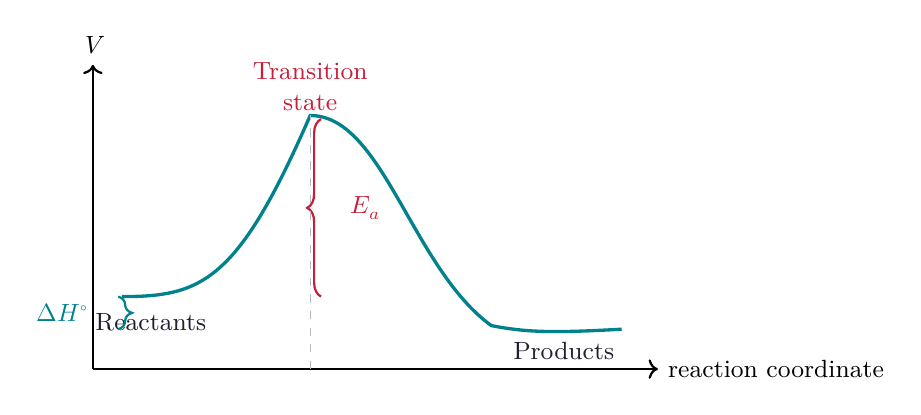
\begin{tikzpicture}[scale=0.92]
  \draw[->, thick] (0,0) -- (7.8,0) node[right, font=\small] {reaction coordinate};
  \draw[->, thick] (0,0) -- (0,4.2) node[above, font=\small] {$V$};
  % energy profile
  \draw[myteal, very thick] (0.4,1.0)
       .. controls (1.5,1.0) and (2.0,1.2) .. (3.0,3.5)
       .. controls (4.0,3.5) and (4.4,1.4) .. (5.5,0.6)
       .. controls (6.0,0.5) and (6.4,0.5) .. (7.3,0.55);
  % reactant/product/TS labels
  \node[font=\small, color=mydark] at (0.8, 0.65) {Reactants};
  \node[font=\small, color=myred,  align=center] at (3.0, 3.9) {Transition\\state};
  \node[font=\small, color=mydark] at (6.5, 0.25) {Products};
  % activation energy brace
  \draw[decorate, decoration={brace, amplitude=5pt}, myred, thick]
       (3.15,1.0) -- (3.15,3.45)
       node[midway, right=7pt, font=\small, color=myred] {$E_a$};
  % delta H brace
  \draw[decorate, decoration={brace, amplitude=5pt, mirror}, myteal, thick]
       (0.35,0.55) -- (0.35,1.0)
       node[midway, left=7pt, font=\small, color=myteal] {$\Delta H^\circ$};
  % dashed vertical at TS
  \draw[dashed, mgframe] (3.0,0) -- (3.0,3.5);
\end{tikzpicture}
\end{tcolorbox}

\textbf{Key features of a PES:}
\begin{itemize}[leftmargin=*, itemsep=2pt, topsep=2pt]
  \item \textbf{Minima} = stable molecules (reactants, products, intermediates).
  \item \textbf{Saddle points} = transition states (highest energy along the reaction path).
  \item \textbf{Activation energy} $E_a$ = energy barrier from reactants to the saddle point.
  \item \textbf{Reaction enthalpy} $\Delta H^\circ$ = difference in energy between reactants and products.
  \item An \emph{exothermic} reaction has products at lower energy; \emph{endothermic} has products higher.
\end{itemize}

\subsection{Transition State Theory (Activated Complex Theory)}
Transition state theory (TST, Eyring, 1935) treats the saddle-point configuration as a quasi-equilibrium ``activated complex'' $[\mathrm{ABC}]^\ddagger$.

\begin{tcolorbox}[formulabox, title={Eyring Rate Equation}]
\[
k = \frac{k_B T}{h}\,e^{-\Delta G^\ddagger/RT} = \frac{k_B T}{h}\,e^{\Delta S^\ddagger/R}\,e^{-\Delta H^\ddagger/RT}
\]
$\Delta G^\ddagger, \Delta H^\ddagger, \Delta S^\ddagger$ are the free energy, enthalpy, and entropy of activation.\\
The factor $k_B T/h \approx 6.3\times10^{12}\ \mathrm{s^{-1}}$ at 298 K is the attempt frequency.
\end{tcolorbox}

\textbf{Connection to Arrhenius:} Comparing with $k=A\,e^{-E_a/RT}$ gives $E_a \approx \Delta H^\ddagger + RT$ and the pre-exponential factor $A = (k_BT/h)\,e^{1+\Delta S^\ddagger/R}$.

\begin{tcolorbox}[exambox, title={Exam Points (Section 2)}]
\begin{itemize}[leftmargin=*, itemsep=2pt, topsep=2pt]
  \item Draw the LJ potential; label $\sigma$, $\varepsilon$, $r_e = 2^{1/6}\sigma$.
  \item At $r_e$: $V$ minimum, $F=0$. For $r<r_e$: repulsion. For $r>r_e$: attraction.
  \item Morse potential adds anharmonicity and dissociation — improves on harmonic oscillator.
  \item On a PES: minima = stable species, saddle points = transition states.
  \item Eyring equation: $k = (k_BT/h)\exp(-\Delta G^\ddagger/RT)$.
\end{itemize}
\end{tcolorbox}

% ===============================================================================
\section{Equations of State for Real Gases}
% ===============================================================================

\begin{tcolorbox}[defbox]
An \textbf{equation of state} (EOS) is a mathematical relationship between the state variables $P$, $V$, $T$, and $n$ of a substance. The ideal gas law ($PV = nRT$) is the simplest EOS but fails at high pressure and low temperature. \emph{Real-gas} equations of state introduce correction terms that account for finite molecular size and intermolecular attractions.
\end{tcolorbox}

\subsection{The Ideal Gas Law and Its Assumptions}
The ideal gas law rests on two assumptions that break down at real conditions:
\begin{enumerate}[leftmargin=*, itemsep=2pt, topsep=2pt]
  \item Molecules are point particles (zero volume).
  \item No intermolecular forces (no attraction or repulsion).
\end{enumerate}

\begin{tcolorbox}[formulabox, title={Ideal Gas Law}]
\[
PV = nRT, \qquad R = 8.314\ \mathrm{J\,mol^{-1}\,K^{-1}} = 0.08206\ \mathrm{L\,atm\,mol^{-1}\,K^{-1}}
\]
\end{tcolorbox}

\subsection{Van der Waals Equation of State}
Van der Waals (1873) introduced two correction parameters:
\begin{itemize}[leftmargin=*, itemsep=2pt, topsep=2pt]
  \item \textbf{$b$ (co-volume):} excluded volume per mole due to finite molecular size. Corrects $V$.
  \item \textbf{$a$ (attraction parameter):} pressure is reduced by attraction, so an internal pressure term $a n^2/V^2$ is added. Corrects $P$.
\end{itemize}

\begin{tcolorbox}[formulabox, title={Van der Waals Equation}]
\[
\boxed{\left(P + \frac{an^2}{V^2}\right)(V - nb) = nRT}
\]
For one mole:
\[
\left(P + \frac{a}{V_m^2}\right)(V_m - b) = RT
\]
$V_m = V/n$ is the molar volume; $a$ in $\mathrm{L^2\,atm\,mol^{-2}}$; $b$ in $\mathrm{L\,mol^{-1}}$.
\end{tcolorbox}

\textbf{Physical interpretation:}
\begin{itemize}[leftmargin=*, itemsep=1pt, topsep=2pt]
  \item $(V_m - b)$: the free volume available to molecules is the total volume minus what the molecules themselves occupy.
  \item $a/V_m^2$: molecules near the wall are pulled back by neighbours --- the measured pressure $P$ is less than the kinetic-theory pressure $P_{\mathrm{kin}}$, so we add back $a/V_m^2$.
\end{itemize}

\begin{tabularx}{\linewidth}{|B{2.4cm}|Y|Y|}
\hline
\textbf{Gas} & \textbf{$a$ (L$^2$ atm mol$^{-2}$)} & \textbf{$b$ (L mol$^{-1}$)} \\
\hline
$\mathrm{H_2}$ & 0.244 & 0.0266 \\
\hline
$\mathrm{N_2}$ & 1.39  & 0.0391 \\
\hline
$\mathrm{CO_2}$ & 3.59 & 0.0427 \\
\hline
$\mathrm{H_2O}$ & 5.46 & 0.0305 \\
\hline
$\mathrm{He}$ & 0.034 & 0.0237 \\
\hline
\end{tabularx}

\begin{tcolorbox}[examplebox, title={Solved Example: Pressure of Real vs Ideal Gas}]
\textbf{Problem:} 1 mol of $\mathrm{CO_2}$ in a $V=1.0\ \mathrm{L}$ container at $T=500\ \mathrm{K}$. Compare ideal and van der Waals pressures.

\textbf{Ideal:}
\[
P_{\mathrm{ideal}} = \frac{RT}{V_m} = \frac{0.08206\times500}{1.0} = 41.0\ \mathrm{atm}
\]
\textbf{Van der Waals} ($a=3.59$, $b=0.0427$):
\[
P = \frac{RT}{V_m - b} - \frac{a}{V_m^2} = \frac{0.08206\times500}{1.0-0.0427} - \frac{3.59}{1.0^2}
= 42.8 - 3.6 = \mathbf{39.2}\ \mathrm{atm}
\]
The real gas pressure is lower because the net effect of attractions ($a$) exceeds the volume correction ($b$) at this condition.
\end{tcolorbox}

\subsection{Compressibility Factor Z}
\begin{tcolorbox}[formulabox, title={Compressibility Factor}]
\[
Z = \frac{PV_m}{RT} = \frac{PV}{nRT}
\]
Ideal gas: $Z = 1$ at all $P$.\\
Real gas: $Z < 1$ when attractions dominate (usually at low--moderate $P$).\\
Real gas: $Z > 1$ when finite volume (repulsion) dominates (very high $P$).
\end{tcolorbox}

\begin{tcolorbox}[tikzbox, title={Compressibility Factor vs Pressure for Real Gases}]
\centering
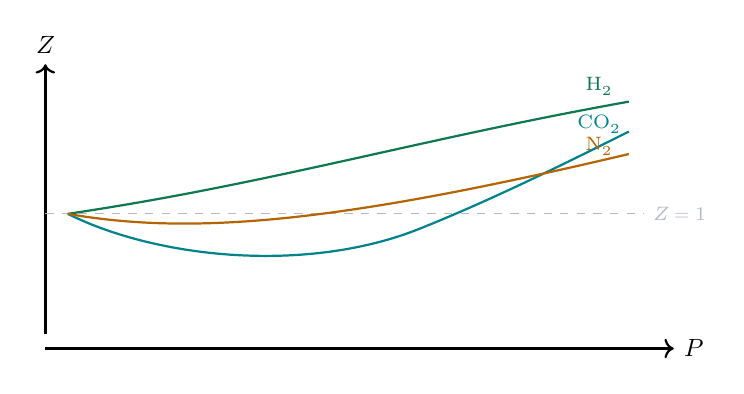
\begin{tikzpicture}[scale=0.95]
  \draw[->, thick] (0,0) -- (8.4,0) node[right, font=\small] {$P$};
  \draw[->, thick] (0,0.2) -- (0,3.8) node[above, font=\small] {$Z$};
  % Z=1 dashed
  \draw[dashed, mgframe] (0.0,1.8) -- (8.0,1.8) node[right, font=\scriptsize] {$Z=1$};
  % H2 (always > 1 at moderate P)
  \draw[mygreen, thick] (0.3,1.8) .. controls (3,2.2) and (5,2.8) .. (7.8,3.3);
  \node[mygreen, font=\scriptsize] at (7.4,3.5) {$\mathrm{H_2}$};
  % CO2 (dips below then rises)
  \draw[myteal, thick] (0.3,1.8) .. controls (1.5,1.2) and (3.5,1.0) .. (5.0,1.6)
       .. controls (6.0,2.0) and (7.0,2.5) .. (7.8,2.9);
  \node[myteal, font=\scriptsize] at (7.4,3.0) {$\mathrm{CO_2}$};
  % N2
  \draw[myamber, thick] (0.3,1.8) .. controls (2.0,1.5) and (4.0,1.7) .. (7.8,2.6);
  \node[myamber, font=\scriptsize] at (7.4,2.7) {$\mathrm{N_2}$};
\end{tikzpicture}
\end{tcolorbox}

\subsection{Virial Equation of State}
The virial equation expresses $Z$ as a power series in density $1/V_m$:

\begin{tcolorbox}[formulabox, title={Virial Equation of State}]
\[
Z = \frac{PV_m}{RT} = 1 + \frac{B}{V_m} + \frac{C}{V_m^2} + \cdots
\]
$B$ = second virial coefficient (accounts for pair interactions), $C$ = third virial coefficient. For the van der Waals gas at low density: $B = b - a/(RT)$.\\
At the Boyle temperature $T_B$: $B = 0$ so $Z \approx 1$ at low--moderate pressure.
\end{tcolorbox}

\subsection{Other Equations of State}

\begin{tabularx}{\linewidth}{|B{2.6cm}|Y|Y|}
\hline
\textbf{EOS} & \textbf{Expression (1 mol)} & \textbf{Improvement over VdW} \\
\hline
Dieterici & $P(V_m-b)=RT\,e^{-a/RTV_m}$ & Better near critical point \\
\hline
Redlich--Kwong & $P=\displaystyle\frac{RT}{V_m-b}-\frac{a}{T^{1/2}V_m(V_m+b)}$ & Better for gas-phase calculations \\
\hline
Peng--Robinson & Modified cubic with two parameters & Used in petroleum engineering \\
\hline
Ideal gas & $PV_m = RT$ & Reference baseline \\
\hline
\end{tabularx}

\subsection{Boyle Temperature}
At the Boyle temperature, the second virial coefficient $B = 0$, so the gas behaves nearly ideally over a range of pressures.

\begin{tcolorbox}[formulabox, title={Boyle Temperature for a van der Waals Gas}]
\[
T_B = \frac{a}{Rb}
\]
\end{tcolorbox}

\begin{tcolorbox}[examplebox, title={Solved Example: Boyle Temperature of \texorpdfstring{$\mathrm{CO_2}$}{CO2}}]
$a=3.59\ \mathrm{L^2\,atm\,mol^{-2}}$, $b=0.0427\ \mathrm{L\,mol^{-1}}$:
\[
T_B = \frac{3.59}{0.08206\times0.0427} = \frac{3.59}{0.003504} = 1024\ \mathrm{K}
\]
Below $T_B$ (1024 K for $\mathrm{CO_2}$), attractions dominate and $Z<1$ at modest pressures.
\end{tcolorbox}

\subsection{Joule--Thomson Effect}
When a real gas expands irreversibly through a porous plug (throttle) from high pressure to low, the process is isenthalpic ($\Delta H = 0$). The temperature may rise or fall.

\begin{tcolorbox}[formulabox, title={Joule--Thomson Coefficient}]
\[
\mu_{\mathrm{JT}} = \left(\frac{\partial T}{\partial P}\right)_H
\]
For a van der Waals gas at low density:
\[
\mu_{\mathrm{JT}} \approx \frac{1}{C_P}\!\left(\frac{2a}{RT} - b\right)
\]
\textbf{At $T < T_i$ (inversion temperature):} $\mu_{\mathrm{JT}} > 0$, gas cools on expansion.\\
\textbf{At $T > T_i$:} $\mu_{\mathrm{JT}} < 0$, gas warms on expansion.
\end{tcolorbox}

\begin{tabularx}{\linewidth}{|B{3.0cm}|Y|Y|}
\hline
\textbf{Condition} & \textbf{$\mu_{\mathrm{JT}}$} & \textbf{Effect} \\
\hline
$T < T_i$ & Positive & Cooling (used in liquefaction) \\
\hline
$T = T_i$ & Zero & No temperature change \\
\hline
$T > T_i$ & Negative & Heating \\
\hline
\end{tabularx}

\textbf{Inversion temperature:} $T_i = 2a/(Rb)$. Note $T_i = 2T_B$. For $\mathrm{N_2}$: $T_i\approx 621\ \mathrm{K}$, so pre-cooling is needed before throttling to liquefy nitrogen. For $\mathrm{H_2}$ and $\mathrm{He}$: $T_i$ is below room temperature, so they warm on throttling without pre-cooling.

\begin{tcolorbox}[masonbox, title={Linde Liquefaction Process and Joule--Thomson Effect}]
The Linde process uses the Joule--Thomson effect to liquefy air: compressed gas expands through a throttle valve, cools, is recycled back, and after many cycles reaches the liquefaction temperature. Gas must be pre-cooled below its inversion temperature first. This principle is used to produce liquid $\mathrm{N_2}$ ($77\ \mathrm{K}$), liquid $\mathrm{O_2}$ ($90\ \mathrm{K}$), and liquid air for cryogenics.
\end{tcolorbox}

\begin{tcolorbox}[exambox, title={Exam Points (Section 3)}]
\begin{itemize}[leftmargin=*, itemsep=2pt, topsep=2pt]
  \item Van der Waals: $a$ corrects $P$ (attractions), $b$ corrects $V$ (molecular size).
  \item Solve $P = RT/(V_m-b) - a/V_m^2$ numerically in 5-mark problems.
  \item $Z < 1$: attraction-dominated; $Z > 1$: repulsion-dominated.
  \item Boyle temperature: $T_B = a/(Rb)$; $B = 0$ there.
  \item Joule--Thomson: isenthalpic expansion; $\mu_{\mathrm{JT}} > 0$ below inversion temperature.
  \item Inversion temperature: $T_i = 2a/(Rb) = 2T_B$.
\end{itemize}
\end{tcolorbox}

% ===============================================================================
\section{Critical Phenomena and the Continuity of State}
% ===============================================================================

\begin{tcolorbox}[defbox]
\textbf{Critical phenomena} describe the behaviour of substances at the \emph{critical point} --- the unique temperature $T_c$, pressure $P_c$, and molar volume $V_c$ at which the liquid--vapour interface vanishes and liquid and vapour become identical. Above $T_c$, no amount of pressure can liquefy the gas.
\end{tcolorbox}

\subsection{Phase Diagram and the Liquid--Vapour Boundary}

\begin{tcolorbox}[tikzbox, title={Pressure--Temperature Phase Diagram}]
\centering
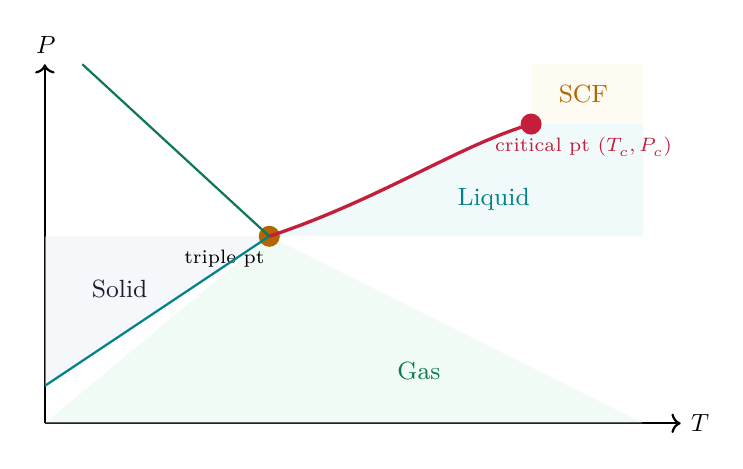
\begin{tikzpicture}[scale=0.95]
  \draw[->, thick] (0,0) -- (8.5,0) node[right, font=\small] {$T$};
  \draw[->, thick] (0,0) -- (0,4.8) node[above, font=\small] {$P$};
  % Solid region
  \fill[hdrgray, opacity=0.5] (0,0.5)--(3.0,2.5)--(0,2.5)--cycle;
  \node[font=\small, color=mydark] at (1.0,1.8) {Solid};
  % Liquid region
  \fill[hdrteal, opacity=0.4] (3.0,2.5)--(6.5,4.0)--(8.0,4.0)--(8.0,2.5)--cycle;
  \node[font=\small, color=myteal] at (6.0,3.0) {Liquid};
  % Gas region
  \fill[hdrgreen, opacity=0.4] (0,0)--(3.0,2.5)--(8.0,0)--cycle;
  \node[font=\small, color=mygreen] at (5.0,0.7) {Gas};
  % Supercritical
  \fill[hdramber, opacity=0.3] (6.5,4.0)--(8.0,4.0)--(8.0,4.8)--(6.5,4.8)--cycle;
  \node[font=\small, color=myamber] at (7.2,4.4) {SCF};
  % Triple point
  \fill[myamber] (3.0,2.5) circle (4pt);
  \node[font=\scriptsize] at (2.4,2.2) {triple pt};
  % Critical point
  \fill[myred] (6.5,4.0) circle (4pt);
  \node[font=\scriptsize, color=myred] at (7.2,3.7) {critical pt ($T_c,P_c$)};
  % Vapour pressure curve
  \draw[myred, very thick] (3.0,2.5) .. controls (4.5,3.0) and (5.5,3.7) .. (6.5,4.0);
  % Sublimation and fusion curves
  \draw[myteal, thick] (3.0,2.5) -- (0,0.5);
  \draw[mygreen, thick] (3.0,2.5) -- (0.5,4.8);
\end{tikzpicture}
\end{tcolorbox}

\textbf{Key points:}
\begin{itemize}[leftmargin=*, itemsep=1pt, topsep=2pt]
  \item \textbf{Triple point}: all three phases coexist (unique $T$ and $P$). For water: $T_{tr}=273.16\ \mathrm{K}$, $P_{tr}=611.7\ \mathrm{Pa}$.
  \item \textbf{Critical point}: liquid--vapour boundary terminates. Above $T_c$: single supercritical fluid (SCF) phase.
  \item \textbf{Vapour pressure curve}: slope given by Clausius--Clapeyron equation.
\end{itemize}

\subsection{Derivation of Critical Constants from the Van der Waals Equation}

\begin{tcolorbox}[formulabox, title={Conditions at the Critical Point}]
At the critical point, the isotherm has an inflection point with zero slope:
\[
\left(\frac{\partial P}{\partial V_m}\right)_{T_c} = 0
\qquad\text{and}\qquad
\left(\frac{\partial^2 P}{\partial V_m^2}\right)_{T_c} = 0
\]
\end{tcolorbox}

Starting from the van der Waals EOS for 1 mol:
\[
P = \frac{RT}{V_m - b} - \frac{a}{V_m^2}
\]

First derivative:
\[
\frac{\partial P}{\partial V_m} = -\frac{RT}{(V_m-b)^2} + \frac{2a}{V_m^3} = 0
\quad\Rightarrow\quad RT(V_m-b)^2 = 2a\,\frac{(V_m-b)^2\,(V_m-b)}{V_m^3}\cdot V_m^3 \tag{i}
\]

Second derivative:
\[
\frac{\partial^2 P}{\partial V_m^2} = \frac{2RT}{(V_m-b)^3} - \frac{6a}{V_m^4} = 0
\quad\Rightarrow\quad RT(V_m-b)^3 = 3a\cdot\frac{(V_m-b)^3}{V_m^4}\cdot V_m^4 \tag{ii}
\]

Dividing (ii) by (i):
\[
\frac{(V_m-b)}{1} = \frac{3}{2}V_m \quad\Rightarrow\quad 2V_m - 2b = 3V_m \quad\Rightarrow\quad \boxed{V_c = 3b}
\]

Substituting back into (i):
\[
RT_c = \frac{2a(V_c-b)^2}{V_c^3} = \frac{2a(2b)^2}{(3b)^3} = \frac{8a}{27b}
\quad\Rightarrow\quad \boxed{T_c = \frac{8a}{27Rb}}
\]

And using the VdW EOS at the critical point:
\[
\boxed{P_c = \frac{a}{27b^2}}
\]

\begin{tcolorbox}[formulabox, title={Critical Constants (Van der Waals)}]
\[
V_c = 3b, \qquad T_c = \frac{8a}{27Rb}, \qquad P_c = \frac{a}{27b^2}
\]
Also useful: $\displaystyle\frac{P_c V_c}{RT_c} = \frac{3}{8} = 0.375$\quad (critical compression factor for a VdW gas).
\end{tcolorbox}

\begin{tcolorbox}[examplebox, title={Solved Example: Critical Constants of \texorpdfstring{$\mathrm{N_2}$}{N2}}]
$a=1.39\ \mathrm{L^2\,atm\,mol^{-2}}$, $b=0.0391\ \mathrm{L\,mol^{-1}}$:
\[
V_c = 3(0.0391) = 0.117\ \mathrm{L\,mol^{-1}}
\]
\[
T_c = \frac{8(1.39)}{27(0.08206)(0.0391)} = \frac{11.12}{0.08661} = 128.4\ \mathrm{K}
\]
\[
P_c = \frac{1.39}{27(0.0391)^2} = \frac{1.39}{0.04128} = 33.7\ \mathrm{atm}
\]
Experimental: $T_c=126.2\ \mathrm{K}$, $P_c=33.9\ \mathrm{atm}$ --- excellent agreement.
\end{tcolorbox}

\subsection{Reduced Variables and the Law of Corresponding States}

\begin{tcolorbox}[defbox]
\textbf{Reduced variables} express $T$, $P$, and $V$ as fractions of their critical values:
\[
T_r = \frac{T}{T_c}, \qquad P_r = \frac{P}{P_c}, \qquad V_r = \frac{V_m}{V_c}
\]
\textbf{Law of Corresponding States (van der Waals):} All gases obey the \emph{same} equation of state when expressed in terms of reduced variables, regardless of their identity.
\end{tcolorbox}

Substituting into the van der Waals equation:
\[
\left(P_r + \frac{3}{V_r^2}\right)\!\left(V_r - \frac{1}{3}\right) = \frac{8}{3}T_r
\]
This \emph{reduced van der Waals equation} has no gas-specific parameters. It predicts that at the same $T_r$ and $P_r$, all gases have the same $Z$ --- the basis of \emph{generalised compressibility charts} used in engineering.

\begin{tcolorbox}[examplebox, title={Application: Comparing States of Different Gases}]
$\mathrm{CO_2}$ at $T=340\ \mathrm{K}$, $P=100\ \mathrm{atm}$ has $T_r=340/304=1.12$ and $P_r=100/72.9=1.37$.\\
$\mathrm{CH_4}$ at $T=215\ \mathrm{K}$, $P=63.5\ \mathrm{atm}$ has $T_r=215/191=1.12$ and $P_r=63.5/46.1=1.38$.\\
By the law of corresponding states, both gases have approximately the same $Z$ even though their absolute conditions differ.
\end{tcolorbox}

\subsection{Andrews Isotherms and the Critical Region}

\begin{tcolorbox}[tikzbox, title={$P$--$V_m$ Isotherms of a Real Gas (Andrews-Type)}]
\centering
\begin{tikzpicture}[scale=0.95]
  \draw[->, thick] (0,0) -- (8.5,0) node[right, font=\small] {$V_m$};
  \draw[->, thick] (0,0) -- (0,4.8) node[above, font=\small] {$P$};
  % Isotherm T >> Tc (nearly ideal)
  \draw[mygreen, thick, domain=1.0:8.0, smooth, variable=\x]
       plot (\x, {3.0/\x+0.3}) node[right, font=\scriptsize, color=mygreen] {$T \gg T_c$};
  % Isotherm T > Tc
  \draw[myteal, thick, domain=0.8:8.0, smooth, variable=\x]
       plot (\x, {2.0/\x+0.15}) node[right, font=\scriptsize, color=myteal] {$T > T_c$};
  % Critical isotherm
  \draw[myred, very thick, domain=0.65:8.0, smooth, variable=\x]
       plot (\x, {2.9*exp(-0.6*(\x-1.5))^3 - 1.0*exp(-0.3*(\x-1.5))+1.2})
       node[right, font=\scriptsize, color=myred] {$T = T_c$};
  % Critical point
  \fill[myred] (1.5,1.2) circle (4pt);
  \node[myred, font=\scriptsize, anchor=south] at (1.8,1.4) {CP};
  % Subcritical isotherm with horizontal portion
  \draw[mypurple, thick] (0.5,2.5)--(0.8,2.5);
  \draw[mypurple, thick] (0.8,2.5) -- (4.2,2.5);
  \draw[mypurple, thick] (4.2,2.5)--(4.2,0.6);
  \draw[mypurple, thick, domain=4.2:8.0, smooth, variable=\x]
       plot (\x, {0.6/(\x-0.1)+0.1});
  \node[mypurple, font=\scriptsize] at (2.5,2.8) {$T < T_c$ (two-phase)};
\end{tikzpicture}
\end{tcolorbox}

\textbf{Reading the isotherms:}
\begin{itemize}[leftmargin=*, itemsep=2pt, topsep=2pt]
  \item Above $T_c$: smooth curves, gas cannot be liquefied.
  \item At $T_c$: inflection point at the critical point (critical isotherm).
  \item Below $T_c$: isotherms show a \emph{horizontal portion} where liquid and vapour coexist at constant $P$ (vapour pressure). Compression reduces volume along this plateau until all vapour condenses.
\end{itemize}

\subsection{Clausius--Clapeyron Equation}
Along the vapour-pressure curve, the slope $dP/dT$ is given by the Clausius--Clapeyron equation.

\begin{tcolorbox}[formulabox, title={Clausius--Clapeyron Equation}]
\[
\frac{dP}{dT} = \frac{\Delta H_{\mathrm{vap}}}{T\,\Delta V_{\mathrm{vap}}}
\quad\xrightarrow{\text{ideal gas approx.}}\quad
\frac{d\ln P}{dT} = \frac{\Delta H_{\mathrm{vap}}}{RT^2}
\]
Integrated form:
\[
\ln\frac{P_2}{P_1} = -\frac{\Delta H_{\mathrm{vap}}}{R}\!\left(\frac{1}{T_2}-\frac{1}{T_1}\right)
\]
A plot of $\ln P$ vs $1/T$ is linear with slope $-\Delta H_{\mathrm{vap}}/R$.
\end{tcolorbox}

\begin{tcolorbox}[examplebox, title={Solved Example: Vapour Pressure of Water}]
Water has $\Delta H_{\mathrm{vap}}=40.7\ \mathrm{kJ\,mol^{-1}}$. At $T_1=373\ \mathrm{K}$, $P_1=1\ \mathrm{atm}$. Find $P$ at $T_2=393\ \mathrm{K}$.
\[
\ln\frac{P_2}{1} = -\frac{40700}{8.314}\!\left(\frac{1}{393}-\frac{1}{373}\right)
= -4893\times(-1.364\times10^{-4}) = 0.668
\]
\[
P_2 = e^{0.668} = 1.95\ \mathrm{atm}
\]
The vapour pressure nearly doubles from $373\ \mathrm{K}$ to $393\ \mathrm{K}$, consistent with the rapid increase seen in pressure cookers.
\end{tcolorbox}

\subsection{Supercritical Fluids}
Above $T_c$ and $P_c$ the distinction between liquid and gas vanishes. The substance is a \textbf{supercritical fluid (SCF)} with properties intermediate between liquid and gas.

\begin{tabularx}{\linewidth}{|B{2.6cm}|Y|Y|Y|}
\hline
\textbf{Property} & \textbf{Gas} & \textbf{SCF} & \textbf{Liquid} \\
\hline
Density & Low & Liquid-like & High \\
\hline
Diffusivity & High & Intermediate & Low \\
\hline
Viscosity & Low & Low & High \\
\hline
Solvation & Negligible & Tunable & Fixed \\
\hline
\end{tabularx}

\textbf{Critical constants of common SCF solvents:}\par\noindent
\begin{tabularx}{\linewidth}{|B{2.4cm}|Y|Y|Y|}
\hline
\textbf{Solvent} & \textbf{$T_c$ (K)} & \textbf{$P_c$ (bar)} & \textbf{Applications} \\
\hline
$\mathrm{CO_2}$ & 304 & 73.8 & Decaffeination, dry cleaning, drug extraction \\
\hline
$\mathrm{H_2O}$ & 647 & 220.9 & Oxidation of organic waste, hydrothermal synthesis \\
\hline
$\mathrm{CH_4}$ & 191 & 46.1 & Natural gas processing \\
\hline
Ethanol & 516 & 63.8 & Food industry extraction \\
\hline
\end{tabularx}

\begin{tcolorbox}[masonbox, title={Why \texorpdfstring{$\mathrm{sc}$-$\mathrm{CO_2}$}{sc-CO2} is the Industrial SCF of Choice}]
Supercritical $\mathrm{CO_2}$ has $T_c=304\ \mathrm{K}$ (near room temperature) and $P_c=73.8\ \mathrm{bar}$ (accessible with standard pumps). It is non-toxic, non-flammable, cheap, and leaves no solvent residue. Its solvating power is tunable by pressure, making it ideal for pharmaceutical extraction, polymer processing, and green chemistry.
\end{tcolorbox}

\begin{tcolorbox}[exambox, title={Exam Points (Section 4)}]
\begin{itemize}[leftmargin=*, itemsep=2pt, topsep=2pt]
  \item Derive $V_c=3b$, $T_c=8a/27Rb$, $P_c=a/27b^2$ from the VdW conditions at CP.
  \item Critical compression factor: $Z_c = P_cV_c/RT_c = 3/8$.
  \item Law of corresponding states: all gases follow the same reduced VdW EOS.
  \item Andrews isotherms: identify two-phase region, critical point, and supercritical region.
  \item Clausius--Clapeyron: $\ln(P_2/P_1) = -(\Delta H_{\mathrm{vap}}/R)(1/T_2 - 1/T_1)$.
  \item SCF properties: liquid-like density, gas-like diffusivity; CO$_2$ example.
\end{itemize}
\end{tcolorbox}

% ===============================================================================
\section{Applications of Intermolecular Forces and Real-Gas Behaviour}
% ===============================================================================

\begin{tcolorbox}[defbox]
Understanding IMFs and real-gas equations of state is not purely theoretical --- they govern physical properties and underpin industrial processes from gas liquefaction to drug design.
\end{tcolorbox}

\subsection{Effect of IMFs on Physical Properties}

\begin{tabularx}{\linewidth}{|B{3.0cm}|Y|Y|}
\hline
\textbf{Property} & \textbf{How IMF controls it} & \textbf{Example} \\
\hline
Boiling point & Stronger IMF $\Rightarrow$ more energy to vaporise & $\mathrm{H_2O}$ (100$^\circ$C) vs $\mathrm{H_2S}$ ($-60^\circ$C) \\
\hline
Melting point & Stronger crystal forces $\Rightarrow$ higher mp & NaCl (801$^\circ$C) vs Ar ($-189^\circ$C) \\
\hline
Viscosity & Larger/polar molecules have stronger IMF $\Rightarrow$ more resistance to flow & Glycerol $\gg$ water \\
\hline
Surface tension & IMF pulling surface molecules inward & Water (72 mN m$^{-1}$) $\gg$ hexane (18 mN m$^{-1}$) \\
\hline
Solubility & Like-dissolves-like: matching IMF types & NaCl in water, iodine in CCl$_4$ \\
\hline
Heat of vaporisation & Energy to overcome IMF & Water $44\ \mathrm{kJ\,mol^{-1}}$, hexane $31\ \mathrm{kJ\,mol^{-1}}$ \\
\hline
\end{tabularx}

\subsection{Like-Dissolves-Like Rule}
\begin{tcolorbox}[defbox]
\textbf{Like dissolves like:} A solute dissolves in a solvent when the solvent--solute interactions are comparable in type and strength to the solvent--solvent interactions. Polar solutes dissolve in polar solvents; non-polar solutes dissolve in non-polar solvents.
\end{tcolorbox}

\textbf{Thermodynamic justification:} Dissolution is spontaneous when $\Delta G_{\mathrm{solvation}} < 0$. This requires $\Delta H_{\mathrm{solvation}} \approx -(\Delta H_{\mathrm{lattice/assoc}} + \Delta H_{\mathrm{solvent\ cavity}})$, which holds when IMF types match.

\subsection{Hydrogen Bonding in Biological Systems}
\begin{itemize}[leftmargin=*, itemsep=2pt, topsep=2pt]
  \item \textbf{DNA base pairing:} A--T has 2 H-bonds ($20\ \mathrm{kJ\,mol^{-1}}$); G--C has 3 ($30\ \mathrm{kJ\,mol^{-1}}$). Collectively they stabilise the double helix.
  \item \textbf{Protein folding:} H-bonds between backbone N--H and C$=$O groups stabilise $\alpha$-helices and $\beta$-sheets.
  \item \textbf{Enzyme catalysis:} H-bonds in the active site position substrates precisely.
  \item \textbf{Membrane fluidity:} Phospholipid bilayers rely on London forces between non-polar tails, H-bonds between polar heads and water.
\end{itemize}

\subsection{Gas Liquefaction and Industrial Gases}
Liquefying a gas requires cooling it below its critical temperature and then compressing it. The Joule--Thomson effect is harnessed industrially.

\begin{tcolorbox}[tikzbox, title={Linde Liquefaction Cycle (Schematic)}]
\centering
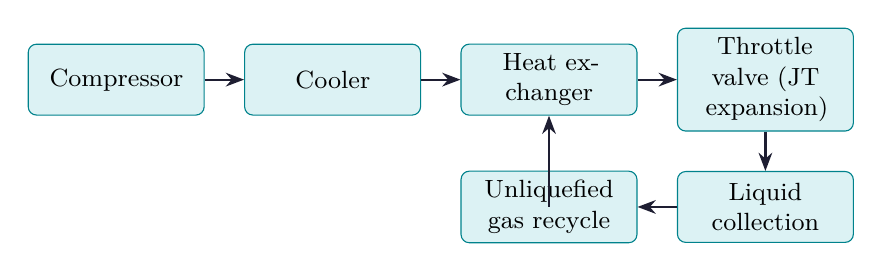
\begin{tikzpicture}[node distance=0.3cm and 0.4cm,
  sblock/.style={rectangle, draw=myteal, fill=hdrteal, text width=2.0cm,
    align=center, minimum height=0.9cm, font=\small, rounded corners=3pt}]
  \node[sblock] (n1) {Compressor};
  \node[sblock, right=0.5cm of n1] (n2) {Cooler};
  \node[sblock, right=0.5cm of n2] (n3) {Heat exchanger};
  \node[sblock, right=0.5cm of n3] (n4) {Throttle valve (JT expansion)};
  \node[sblock, below=0.5cm of n4] (n5) {Liquid collection};
  \node[sblock, left=0.5cm of n5] (n6) {Unliquefied gas recycle};
  \draw[arrow] (n1)--(n2);
  \draw[arrow] (n2)--(n3);
  \draw[arrow] (n3)--(n4);
  \draw[arrow] (n4)--(n5);
  \draw[arrow] (n5)--(n6);
  \draw[arrow] (n6)-|(n3);
\end{tikzpicture}
\end{tcolorbox}

\textbf{Industrial cryogens and their $T_c$:}
\begin{itemize}[leftmargin=*, itemsep=1pt, topsep=2pt]
  \item Liquid $\mathrm{N_2}$ ($77\ \mathrm{K}$): $T_c=126\ \mathrm{K}$, pre-cooling to $\sim100\ \mathrm{K}$ needed.
  \item Liquid $\mathrm{O_2}$ ($90\ \mathrm{K}$): $T_c=155\ \mathrm{K}$.
  \item Liquid $\mathrm{He}$ ($4.2\ \mathrm{K}$): $T_c=5.2\ \mathrm{K}$, requires liquid $\mathrm{N_2}$ pre-cool then JT expansion.
  \item Liquid $\mathrm{H_2}$ ($20\ \mathrm{K}$): $T_c=33\ \mathrm{K}$, must pre-cool below inversion temperature.
\end{itemize}

\subsection{Real Gases in Engineering Calculations}
Van der Waals and virial equations are used in:
\begin{itemize}[leftmargin=*, itemsep=1pt, topsep=2pt]
  \item Pipeline sizing for high-pressure natural gas ($Z\neq1$).
  \item Refrigeration cycle analysis (refrigerant properties near $T_c$).
  \item Supercritical extraction unit design.
  \item Prediction of dew points and bubble points in process engineering.
\end{itemize}

\subsection{Colligative Properties: IMF Context}
Though formally under solution chemistry, colligative properties arise from the modification of solvent--solvent IMFs by added solute.

\begin{tabularx}{\linewidth}{|B{3.0cm}|Y|Y|}
\hline
\textbf{Property} & \textbf{IMF connection} & \textbf{Equation} \\
\hline
Boiling-point elevation & Solute lowers solvent vapour pressure $\Rightarrow$ higher bp & $\Delta T_b = K_b\,m$ \\
\hline
Freezing-point depression & Solute disrupts lattice IMF network & $\Delta T_f = K_f\,m$ \\
\hline
Osmotic pressure & Solute concentration drives solvent flow across membrane & $\pi = iMRT$ \\
\hline
Raoult's law & Vapour pressure lowering $\Delta P = x_{\mathrm{sol}}P^\circ$ & Based on ideal mixing of IMFs \\
\hline
\end{tabularx}

\begin{tcolorbox}[exambox, title={Exam Points (Section 5)}]
\begin{itemize}[leftmargin=*, itemsep=2pt, topsep=2pt]
  \item Boiling point order: relates directly to IMF strength (H-bond $>$ dipole $>$ London).
  \item Like-dissolves-like: IMF type determines solubility.
  \item DNA A--T: 2 H-bonds; G--C: 3 H-bonds --- explains higher $T_m$ of GC-rich DNA.
  \item Linde process: compressor $\to$ cooler $\to$ heat exchanger $\to$ throttle (JT cooling) $\to$ liquid.
  \item Clausius--Clapeyron gives slope of vapour-pressure curve; use to find $\Delta H_{\mathrm{vap}}$.
\end{itemize}
\end{tcolorbox}

% ===============================================================================
\newpage
\begin{center}
  {\large\bfseries\color{myred} Quick Revision --- Module 3}\\[3pt]
  {\small\color{mydark} Intermolecular Forces, Real Gases and Critical Phenomena $|$ BS-CH101}
\end{center}
\noindent{\color{myred}\rule{\linewidth}{1.2pt}}
\vspace{4pt}

\begin{tcolorbox}[formulabox, breakable, title={Key Formulas at a Glance},
  title after break={\textbf{Key Formulas at a Glance (contd.)}}]
{\renewcommand{\arraystretch}{1.55}
\begin{tabularx}{\linewidth}{|B{4.6cm}|Y|}
\hline
\textbf{Formula} & \textbf{Meaning} \\
\hline
$V_{\mathrm{ion-ion}} = -\displaystyle\frac{z_1 z_2 e^2}{4\pi\varepsilon_0 r}$ & Coulomb energy between two ions ($\propto r^{-1}$). \\
\hline
$\mu = q\cdot d$ & Dipole moment; 1 D $= 3.336\times10^{-30}\ \mathrm{C\,m}$. \\
\hline
$V_{\mathrm{Keesom}} \propto -\displaystyle\frac{\mu^4}{k_BT\,r^6}$ & Dipole--dipole (thermal-averaged); $r^{-6}$, $T$-dependent. \\
\hline
$V_{\mathrm{London}} \propto -\displaystyle\frac{\alpha_1'\alpha_2' I_1 I_2}{r^6(I_1+I_2)}$ & London dispersion; $r^{-6}$, $T$-independent. \\
\hline
$V_{\mathrm{LJ}} = 4\varepsilon\!\left[(\sigma/r)^{12}-(\sigma/r)^6\right]$ & Lennard-Jones 12-6 potential; $r_e=2^{1/6}\sigma$. \\
\hline
$F = -dV/dr$ & Force from potential energy curve. \\
\hline
$V_{\mathrm{Morse}} = D_e[1-e^{-\beta(r-r_e)}]^2$ & Morse bond potential with dissociation limit. \\
\hline
$\left(P+\displaystyle\frac{a}{V_m^2}\right)(V_m-b)=RT$ & Van der Waals EOS (one mole). \\
\hline
$Z = PV_m/RT$ & Compressibility factor; $Z=1$ ideal. \\
\hline
$Z = 1 + B/V_m + C/V_m^2 + \cdots$ & Virial EOS; $B = b - a/(RT)$ for VdW. \\
\hline
\end{tabularx}}
\vspace{3pt}
{\renewcommand{\arraystretch}{1.55}
\begin{tabularx}{\linewidth}{|B{4.6cm}|Y|}
\hline
$T_B = a/(Rb)$ & Boyle temperature ($B=0$, near-ideal). \\
\hline
$V_c = 3b$, $T_c = 8a/27Rb$, $P_c = a/27b^2$ & Critical constants (VdW). \\
\hline
$Z_c = P_cV_c/RT_c = 3/8$ & Critical compressibility factor (VdW). \\
\hline
$T_r = T/T_c$, $P_r = P/P_c$, $V_r = V_m/V_c$ & Reduced variables. \\
\hline
$(P_r+3/V_r^2)(V_r-1/3)=8T_r/3$ & Reduced VdW EOS (universal). \\
\hline
$\mu_{\mathrm{JT}} = (\partial T/\partial P)_H$ & Joule--Thomson coefficient. \\
\hline
$T_i = 2a/(Rb) = 2T_B$ & Inversion temperature. \\
\hline
$\ln(P_2/P_1)=-(\Delta H_{\mathrm{vap}}/R)(1/T_2 - 1/T_1)$ & Clausius--Clapeyron (integrated). \\
\hline
$\Delta T_b = K_b m$; $\Delta T_f = K_f m$; $\pi = iMRT$ & Colligative properties. \\
\hline
\end{tabularx}}
\end{tcolorbox}

\begin{tcolorbox}[defbox, title={One-Line Definitions}]
\begin{itemize}[leftmargin=*, itemsep=2pt, topsep=2pt]
  \item \textbf{Intermolecular force:} Attractive or repulsive force between separate molecules/ions.
  \item \textbf{Dipole moment:} Vector quantity $\mu = qd$; non-zero for asymmetric charge distribution.
  \item \textbf{London dispersion:} IMF due to instantaneous and induced temporary dipoles; exists in all molecules.
  \item \textbf{Keesom interaction:} Thermal-averaged attraction between two permanent dipoles; proportional to $r^{-6}$ and $1/T$.
  \item \textbf{Debye interaction:} Attraction of permanent dipole on an induced dipole; $r^{-6}$, temperature-independent.
  \item \textbf{Hydrogen bond:} Strong directional interaction of H (bonded to F/O/N) with a lone pair; $15$--$40\ \mathrm{kJ\,mol^{-1}}$.
  \item \textbf{Polarisability:} Ease of distortion of an electron cloud by an electric field; increases down a group.
  \item \textbf{Lennard-Jones potential:} Empirical 12-6 pair potential combining repulsion and London dispersion.
  \item \textbf{Equilibrium separation ($r_e$):} Distance at which $V$ is minimum and $F = 0$.
  \item \textbf{Potential energy surface:} Multi-dimensional energy landscape as function of molecular geometry.
  \item \textbf{Transition state:} Saddle point on the PES; highest energy along the reaction path.
  \item \textbf{Activation energy ($E_a$):} Energy barrier separating reactants from transition state.
  \item \textbf{Real gas:} Gas deviating from ideal due to finite molecular volume and attractions.
  \item \textbf{Van der Waals $a$:} Correction for intermolecular attractions (reduces pressure).
  \item \textbf{Van der Waals $b$:} Excluded volume per mole due to finite molecular size (reduces free volume).
  \item \textbf{Compressibility factor ($Z$):} $PV_m/RT$; equals 1 for ideal gas.
  \item \textbf{Virial coefficient $B$:} Second virial coefficient; zero at Boyle temperature.
  \item \textbf{Boyle temperature:} $T_B = a/(Rb)$; gas behaves nearly ideally.
  \item \textbf{Critical temperature ($T_c$):} Highest $T$ at which gas can be liquefied by pressure alone.
  \item \textbf{Critical pressure ($P_c$):} Pressure needed to liquefy gas at $T_c$.
  \item \textbf{Critical point:} State where liquid and vapour become identical; $(T_c, P_c, V_c)$.
  \item \textbf{Reduced variables:} $T_r$, $P_r$, $V_r$; enable law of corresponding states.
  \item \textbf{Law of corresponding states:} All gases obey the same reduced EOS.
  \item \textbf{Joule--Thomson effect:} Temperature change of real gas on isenthalpic expansion through a throttle.
  \item \textbf{Inversion temperature ($T_i$):} $\mu_{\mathrm{JT}} = 0$; $T_i = 2a/(Rb)$.
  \item \textbf{Supercritical fluid:} Phase above $T_c$ and $P_c$ with liquid-like density and gas-like diffusivity.
  \item \textbf{Clausius--Clapeyron equation:} Relates vapour pressure change to temperature via $\Delta H_{\mathrm{vap}}$.
  \item \textbf{Like-dissolves-like:} Solubility is maximised when solute--solvent IMF type matches.
  \item \textbf{Linde process:} Industrial gas liquefaction using Joule--Thomson expansion cycle.
\end{itemize}
\end{tcolorbox}

\begin{tcolorbox}[exambox, title={Frequently Asked / Viva Questions}]
\begin{enumerate}[topsep=0pt, label=\textbf{Q\arabic*.}, itemsep=5pt]
  \item \Q{What are intermolecular forces? Arrange them in increasing strength.}
    Forces between molecules/ions: London $<$ dipole--dipole $<$ H-bond $<$ ion--dipole $<$ ion--ion.
  \item \Q{Why do London forces increase down a noble-gas group?}
    Larger atoms have more electrons and higher polarisability; instantaneous dipoles are stronger.
  \item \Q{Why is $\mathrm{CO_2}$ non-polar despite having polar bonds?}
    Linear geometry makes bond-dipole vectors cancel exactly.
  \item \Q{What is Keesom interaction and why is it temperature-dependent?}
    Dipole--dipole orientation averaged over thermal motion; higher $T$ scrambles alignment, weakening the interaction.
  \item \Q{State the Lennard-Jones potential and identify each term.}
    $V_{\mathrm{LJ}}=4\varepsilon[(\sigma/r)^{12}-(\sigma/r)^6]$; first term: repulsion; second: London attraction.
  \item \Q{What is the equilibrium separation in the LJ potential?}
    $r_e = 2^{1/6}\sigma \approx 1.122\,\sigma$; found by setting $dV/dr = 0$.
  \item \Q{What is a potential energy surface?}
    A multi-dimensional surface showing molecular energy as a function of geometry; minima = stable species, saddle points = transition states.
  \item \Q{Write the van der Waals equation and explain $a$ and $b$.}
    $(P + a/V_m^2)(V_m - b) = RT$; $a$ corrects for attractions (adds to $P$); $b$ corrects for finite molecular volume (subtracts from $V$).
  \item \Q{What does a compressibility factor $Z < 1$ indicate?}
    Attractive forces dominate; gas occupies less volume than ideal.
  \item \Q{State the virial EOS.}
    $Z = 1 + B/V_m + C/V_m^2 + \cdots$; $B$ is zero at the Boyle temperature.
  \item \Q{Derive the Boyle temperature from the VdW EOS.}
    At $T_B$, second virial coefficient $B = b - a/(RT_B) = 0$, giving $T_B = a/(Rb)$.
  \item \Q{Derive the critical constants from the VdW EOS.}
    Set $(\partial P/\partial V_m)_T = 0$ and $(\partial^2 P/\partial V_m^2)_T = 0$; solving gives $V_c=3b$, $T_c=8a/27Rb$, $P_c=a/27b^2$.
  \item \Q{What is the critical compressibility factor for a VdW gas?}
    $Z_c = P_cV_c/RT_c = 3/8 = 0.375$.
  \item \Q{State the law of corresponding states.}
    All gases obey the same reduced EOS $(P_r+3/V_r^2)(V_r-1/3) = 8T_r/3$ when variables are expressed relative to critical values.
  \item \Q{What is the Joule--Thomson effect?}
    Isenthalpic ($\Delta H=0$) expansion of a real gas through a throttle; temperature falls below the inversion temperature, rises above it.
  \item \Q{What is the inversion temperature?}
    $T_i = 2a/(Rb) = 2T_B$; above $T_i$ the JT coefficient is negative (gas warms).
  \item \Q{Why must hydrogen be pre-cooled before JT liquefaction?}
    $T_i(\mathrm{H_2}) \approx 200\ \mathrm{K}$, below room temperature; at room temperature $\mu_{\mathrm{JT}} < 0$, so H$_2$ warms on throttling.
  \item \Q{State and explain the Clausius--Clapeyron equation.}
    $d\ln P/dT = \Delta H_{\mathrm{vap}}/(RT^2)$; relates slope of vapour-pressure curve to enthalpy of vaporisation; $\ln P$ vs $1/T$ is linear.
  \item \Q{What is a supercritical fluid? Give one industrial example.}
    Fluid above $T_c$ and $P_c$ with tuneable density; supercritical $\mathrm{CO_2}$ ($T_c=304\ \mathrm{K}$, $P_c=73.8\ \mathrm{bar}$) used for caffeine extraction.
  \item \Q{How does hydrogen bonding stabilise the DNA double helix?}
    A--T: 2 H-bonds; G--C: 3 H-bonds; collectively millions of H-bonds along the helix provide thermodynamic stability while remaining individually reversible for replication.
  \item \Q{Why is water anomalous among hydrides?}
    Extensive H-bonding raises bp (100$^\circ$C vs $-60^\circ$C for H$_2$S), increases heat of vaporisation, and makes ice less dense than liquid water.
  \item \Q{What is the Andrews isotherm?}
    $P$--$V_m$ curve of a real gas at various temperatures; shows two-phase plateau below $T_c$ and inflection point at $T_c$.
  \item \Q{Define triple point and critical point.}
    Triple point: coexistence of solid, liquid, and gas at unique $(T_{tr},P_{tr})$. Critical point: end of liquid--vapour boundary at $(T_c,P_c,V_c)$.
\end{enumerate}
\end{tcolorbox}

\begin{tcolorbox}[tikzbox, title={Summary Reference Table --- Module 3}]
\begin{tabularx}{\linewidth}{|B{2.8cm}|Y|Y|Y|}
\hline
\textbf{Topic} & \textbf{Key concept} & \textbf{Key formula} & \textbf{Exam output} \\
\hline
IMF types & 6 types from ionic to London & $V \propto r^{-1}$ to $r^{-6}$ & Strength order + examples \\
\hline
Lennard-Jones & Repulsion + dispersion & $4\varepsilon[(\sigma/r)^{12}-(\sigma/r)^6]$ & Diagram + labels \\
\hline
PES & Energy vs geometry & Saddle point = TS & Reaction-path diagram \\
\hline
Van der Waals & Real-gas corrections & $(P+a/V_m^2)(V_m-b)=RT$ & Worked numerical \\
\hline
Compressibility & Deviation from ideal & $Z=PV_m/RT$ & Z vs $P$ sketch \\
\hline
Boyle temperature & $Z\approx1$, $B=0$ & $T_B=a/(Rb)$ & Calculation \\
\hline
Critical constants & From VdW conditions & $V_c=3b$, $T_c=8a/27Rb$ & Derivation or value \\
\hline
Corresponding states & Universal VdW & $(P_r+3/V_r^2)(V_r-1/3)=8T_r/3$ & State the law \\
\hline
Joule--Thomson & Isenthalpic expansion & $\mu_{\mathrm{JT}}=(\partial T/\partial P)_H$ & Table: $T$ vs $T_i$ \\
\hline
Clausius--Clapeyron & Vapour-pressure slope & $\ln(P_2/P_1)=-\frac{\Delta H}{R}\Delta(1/T)$ & Find $P$ or $\Delta H$ \\
\hline
Supercritical fluid & Above $T_c$, $P_c$ & $T_c(\mathrm{CO_2})=304\ \mathrm{K}$ & Applications \\
\hline
\end{tabularx}
\end{tcolorbox}

\newpage
% ============================================================================
\renewcommand{\moduletitle}{Module 4 --- Free Energy and Equilibria}
\part{Module 4: Free Energy and Chemical Equilibria}
\setcounter{section}{0}
% ============================================================================

% ===============================================================================
\section{First and Second Laws of Thermodynamics}
% ===============================================================================

\begin{tcolorbox}[defbox]
\textbf{Thermodynamics} is the study of energy transformations. The \emph{first law} states that energy is conserved; the \emph{second law} states that any spontaneous process increases the total entropy of the universe. Together they define the direction and limits of all chemical and physical processes.
\end{tcolorbox}

\subsection{System, Surroundings, and Universe}
\begin{tabularx}{\linewidth}{|B{2.4cm}|Y|Y|}
\hline
\textbf{Term} & \textbf{Definition} & \textbf{Types} \\
\hline
System & The part under study & Open (matter + energy exchange), closed (energy only), isolated (neither) \\
\hline
Surroundings & Everything outside the system & Provides or absorbs heat and work \\
\hline
Universe & System + surroundings & Total energy and entropy defined for universe \\
\hline
\end{tabularx}

\subsection{Internal Energy and the First Law}
\begin{tcolorbox}[formulabox, title={First Law of Thermodynamics}]
\[
\Delta U = q + w
\]
$\Delta U$ = change in internal energy; $q$ = heat absorbed by system (positive when absorbed); $w$ = work done on system.\\
For expansion against constant pressure: $w = -P_{\mathrm{ext}}\,\Delta V$.\\
At constant volume: $\Delta U = q_v$.\\
At constant pressure: $q_p = \Delta H = \Delta U + P\Delta V = \Delta U + \Delta n_g RT$ (for ideal gases).
\end{tcolorbox}

\subsection{Enthalpy and Heat Capacity}
\begin{tcolorbox}[formulabox, title={Enthalpy and Heat Capacity Relations}]
\[
H = U + PV \quad\Rightarrow\quad \Delta H = \Delta U + \Delta(PV)
\]
\[
C_P = \left(\frac{\partial H}{\partial T}\right)_P, \qquad C_V = \left(\frac{\partial U}{\partial T}\right)_V, \qquad C_P - C_V = R\ \text{(ideal gas)}
\]
For a process at constant $P$: $q_P = n C_P \Delta T$.\\
For a process at constant $V$: $q_V = n C_V \Delta T$.
\end{tcolorbox}

\subsection{Hess's Law and Standard Enthalpies}
\begin{tcolorbox}[defbox]
\textbf{Hess's law:} The enthalpy change of a reaction is independent of the pathway; only the initial and final states matter. Thermochemical equations can be combined algebraically to find $\Delta H$ of reactions that are difficult to measure directly.
\end{tcolorbox}

\begin{tcolorbox}[tikzbox, title={Hess's Law Energy Cycle for Combustion of Carbon}]
\centering
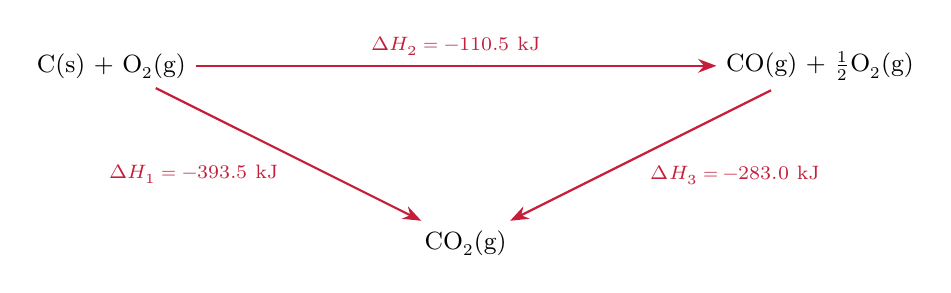
\begin{tikzpicture}[scale=0.9]
  % top-left: C(s) + O2
  \node[font=\small, align=center] (A) at (0,2.5) {C(s) + O$_2$(g)};
  % bottom: CO2(g)
  \node[font=\small, align=center] (B) at (5,0) {CO$_2$(g)};
  % top-right: CO(g) + 1/2 O2
  \node[font=\small, align=center] (C) at (10,2.5) {CO(g) + $\tfrac{1}{2}$O$_2$(g)};
  \draw[redarrow, thick] (A) -- node[below left, font=\scriptsize, color=myred] {$\Delta H_1=-393.5\ \mathrm{kJ}$} (B);
  \draw[redarrow, thick] (A) -- node[above, font=\scriptsize, color=myred] {$\Delta H_2=-110.5\ \mathrm{kJ}$} (C);
  \draw[redarrow, thick] (C) -- node[below right, font=\scriptsize, color=myred] {$\Delta H_3=-283.0\ \mathrm{kJ}$} (B);
\end{tikzpicture}
\end{tcolorbox}

\begin{tcolorbox}[examplebox, title={Solved Example: Hess's Law}]
\textbf{Problem:} Find $\Delta H$ for C(s) + $\tfrac{1}{2}$O$_2$(g) $\to$ CO(g) using:
\begin{enumerate}[leftmargin=*, itemsep=1pt, topsep=1pt]
  \item C(s) + O$_2$(g) $\to$ CO$_2$(g), $\Delta H_1 = -393.5\ \mathrm{kJ\,mol^{-1}}$
  \item CO(g) + $\tfrac{1}{2}$O$_2$(g) $\to$ CO$_2$(g), $\Delta H_2 = -283.0\ \mathrm{kJ\,mol^{-1}}$
\end{enumerate}
\textbf{Solution:} Reverse equation 2 and add:
\[
\Delta H = \Delta H_1 - \Delta H_2 = -393.5 - (-283.0) = -110.5\ \mathrm{kJ\,mol^{-1}}
\]
\end{tcolorbox}

\subsection{Entropy: The Second Law}
\begin{tcolorbox}[defbox]
\textbf{Entropy} $S$ is a state function that measures the dispersal of energy among available microstates. The \textbf{second law} states that for any spontaneous process, $\Delta S_{\mathrm{universe}} = \Delta S_{\mathrm{sys}} + \Delta S_{\mathrm{surr}} > 0$. For a reversible process, $\Delta S_{\mathrm{universe}} = 0$.
\end{tcolorbox}

\begin{tcolorbox}[formulabox, title={Entropy Expressions}]
\[
dS = \frac{\delta q_{\mathrm{rev}}}{T}, \qquad \Delta S = \int_1^2 \frac{\delta q_{\mathrm{rev}}}{T}
\]
For a reversible isothermal expansion of ideal gas: $\Delta S = nR\ln\frac{V_2}{V_1}$.\\
For heating at constant $P$: $\Delta S = nC_P\ln\frac{T_2}{T_1}$.\\
For heating at constant $V$: $\Delta S = nC_V\ln\frac{T_2}{T_1}$.\\
Clausius inequality: $\oint \frac{\delta q}{T} \leq 0$ (equality for reversible cycle).
\end{tcolorbox}

\subsection{Third Law and Absolute Entropy}
\begin{tcolorbox}[defbox]
\textbf{Third law of thermodynamics:} The entropy of a perfect crystalline substance is zero at absolute zero ($S = 0$ at $T = 0\ \mathrm{K}$). This provides an absolute reference scale for entropy.
\end{tcolorbox}

\textbf{Standard molar entropy} $S^\circ$ at 298 K (J mol$^{-1}$ K$^{-1}$):
\begin{tabularx}{\linewidth}{|B{2.6cm}|Y|B{2.6cm}|Y|}
\hline
\textbf{Substance} & \textbf{$S^\circ$} & \textbf{Substance} & \textbf{$S^\circ$} \\
\hline
C(graphite) & 5.7 & H$_2$O(l) & 69.9 \\
\hline
H$_2$(g) & 130.7 & CO$_2$(g) & 213.8 \\
\hline
O$_2$(g) & 205.2 & NaCl(s) & 72.1 \\
\hline
\end{tabularx}

Standard entropy change of reaction: $\Delta S^\circ_{\mathrm{rxn}} = \sum n_p S^\circ(\text{products}) - \sum n_r S^\circ(\text{reactants})$.

\subsection{Work in Reversible and Irreversible Expansion}
This is a 5-mark derivation in nearly every MAKAUT paper.

\begin{tcolorbox}[formulabox, title={Work Done by an Ideal Gas}]
\textbf{Reversible isothermal expansion} (maximum work):
\[
w_{\mathrm{rev}} = -nRT\ln\frac{V_2}{V_1} = -nRT\ln\frac{P_1}{P_2}
\]
\textbf{Irreversible expansion against constant external pressure}:
\[
w_{\mathrm{irrev}} = -P_{\mathrm{ext}}\Delta V = -P_{\mathrm{ext}}(V_2-V_1)
\]
\textbf{Free expansion} (into vacuum, $P_{\mathrm{ext}}=0$): $w = 0$.\\
Rule: $|w_{\mathrm{rev}}| > |w_{\mathrm{irrev}}|$ always — reversible processes deliver maximum work.
\end{tcolorbox}

\begin{tcolorbox}[examplebox, title={Solved Example: Reversible vs Irreversible Work}]
1 mol ideal gas at 300 K expands from $V_1=10\ \mathrm{L}$ to $V_2=30\ \mathrm{L}$.

\textbf{Reversible:}
\[
w_{\mathrm{rev}} = -nRT\ln\frac{V_2}{V_1} = -(1)(8.314)(300)\ln 3 = -2494\times1.099 = -2741\ \mathrm{J}
\]
\textbf{Irreversible} against $P_{\mathrm{ext}} = P_2 = nRT/V_2 = (1)(8.314)(300)/30\times10^{-3} = 83140\ \mathrm{Pa}$:

$w_{\mathrm{irrev}} = -(83140)(30-10)\times10^{-3} = -1663\ \mathrm{J}$

Reversible work ($2741\ \mathrm{J}$) is greater than irreversible work ($1663\ \mathrm{J}$) — confirms second law.
\end{tcolorbox}

\subsection{Entropy of Phase Transition and Trouton's Rule}
At a phase transition (melting, boiling), temperature is constant and heat flows reversibly:
\[
\Delta S_{\mathrm{vap}} = \frac{\Delta H_{\mathrm{vap}}}{T_b}, \qquad \Delta S_{\mathrm{fus}} = \frac{\Delta H_{\mathrm{fus}}}{T_m}
\]
\textbf{Trouton's rule:} For most non-associated liquids, $\Delta S_{\mathrm{vap}} \approx 85\ \mathrm{J\,mol^{-1}\,K^{-1}}$ at the normal boiling point. Water deviates ($\Delta S_{\mathrm{vap}} \approx 109\ \mathrm{J\,mol^{-1}\,K^{-1}}$) because its extensive H-bonding creates extra order in the liquid phase.

\subsection{Kirchhoff's Equation: ΔH Variation with Temperature}
Enthalpy of a reaction changes with temperature because reactant and product heat capacities differ.

\begin{tcolorbox}[formulabox, title={Kirchhoff's Equation}]
\[
\frac{d(\Delta H)}{dT} = \Delta C_P = \sum n_p C_P(\text{products}) - \sum n_r C_P(\text{reactants})
\]
Integrated form (assuming $\Delta C_P$ is constant):
\[
\Delta H_{T_2} = \Delta H_{T_1} + \Delta C_P\,(T_2 - T_1)
\]
\end{tcolorbox}

\begin{tcolorbox}[exambox, title={Exam Points (Section 1)}]
\begin{itemize}[leftmargin=*, itemsep=2pt, topsep=2pt]
  \item First law: $\Delta U = q + w$; at const $P$: $\Delta H = q_P$.
  \item $C_P - C_V = R$ for ideal gas; $\Delta H = \Delta U + \Delta n_g RT$ for gas reactions.
  \item Hess's law: $\Delta H$ is path-independent; combine equations algebraically.
  \item Second law: $\Delta S_{\mathrm{univ}} > 0$ for spontaneous; $= 0$ reversible.
  \item Third law: $S = 0$ at $0\ \mathrm{K}$ for perfect crystal — provides absolute entropy scale.
\end{itemize}
\end{tcolorbox}

% ===============================================================================
\section{Gibbs Free Energy and Spontaneity}
% ===============================================================================

\begin{tcolorbox}[defbox]
\textbf{Gibbs free energy} $G = H - TS$ is the thermodynamic potential that determines spontaneity at constant temperature and pressure. It combines both the enthalpic driving force (energy minimisation) and the entropic driving force (disorder maximisation) into a single criterion.
\end{tcolorbox}

\subsection{Derivation of the Gibbs Free Energy Criterion}
At constant $T$ and $P$, the second law requires $\Delta S_{\mathrm{univ}} \geq 0$. Since $\Delta S_{\mathrm{surr}} = -\Delta H / T$ (heat lost by system is gained by surroundings reversibly):
\[
\Delta S_{\mathrm{univ}} = \Delta S_{\mathrm{sys}} - \frac{\Delta H}{T} \geq 0
\quad\Rightarrow\quad T\Delta S - \Delta H \geq 0
\quad\Rightarrow\quad \Delta H - T\Delta S \leq 0
\]
Defining $\Delta G = \Delta H - T\Delta S$:

\begin{tcolorbox}[formulabox, title={Gibbs Free Energy Criterion}]
\[
\Delta G = \Delta H - T\Delta S
\]
\begin{itemize}[leftmargin=*, itemsep=1pt, topsep=2pt]
  \item $\Delta G < 0$: spontaneous (product-favoured).
  \item $\Delta G = 0$: system at equilibrium.
  \item $\Delta G > 0$: non-spontaneous (reactant-favoured under those conditions).
\end{itemize}
$\Delta G$ equals the maximum non-expansion (useful) work: $w_{\mathrm{max}} = \Delta G$.
\end{tcolorbox}

\subsection{The Four Spontaneity Cases}
The sign of $\Delta G = \Delta H - T\Delta S$ depends on temperature through the entropy term.

\begin{tabularx}{\linewidth}{|B{1.8cm}|B{1.8cm}|Y|Y|}
\hline
\textbf{$\Delta H$} & \textbf{$\Delta S$} & \textbf{Sign of $\Delta G$} & \textbf{Spontaneity} \\
\hline
$-$ & $+$ & Always $-$ & Spontaneous at \textbf{all} temperatures \\
\hline
$+$ & $-$ & Always $+$ & Non-spontaneous at \textbf{all} temperatures \\
\hline
$-$ & $-$ & $-$ at low $T$, $+$ at high $T$ & Spontaneous at \textbf{low} temperature \\
\hline
$+$ & $+$ & $+$ at low $T$, $-$ at high $T$ & Spontaneous at \textbf{high} temperature \\
\hline
\end{tabularx}

\textbf{Crossover temperature} (where $\Delta G = 0$):
\[
T^* = \frac{\Delta H}{\Delta S}
\]

\begin{tcolorbox}[examplebox, title={Solved Example: Crossover Temperature}]
For the decomposition of $\mathrm{CaCO_3}(s) \to \mathrm{CaO}(s) + \mathrm{CO_2}(g)$:
$\Delta H^\circ = +178\ \mathrm{kJ\,mol^{-1}}$, $\Delta S^\circ = +165\ \mathrm{J\,mol^{-1}\,K^{-1}} = +0.165\ \mathrm{kJ\,mol^{-1}\,K^{-1}}$.
\[
T^* = \frac{178}{0.165} = 1079\ \mathrm{K}
\]
Below 1079 K the reaction is non-spontaneous ($\Delta G > 0$); above it becomes spontaneous ($\Delta G < 0$). This explains why limestone kilns operate above $\sim 800^\circ\mathrm{C}$.
\end{tcolorbox}

\subsection{Standard Free Energy of Formation}
\begin{tcolorbox}[defbox]
$\Delta G_f^\circ$ is the Gibbs free energy change when one mole of a compound is formed from its elements in their standard states at 298 K and 1 bar. By definition, $\Delta G_f^\circ = 0$ for all elements in their standard states.
\end{tcolorbox}

\[
\Delta G^\circ_{\mathrm{rxn}} = \sum n_p\,\Delta G_f^\circ(\text{products}) - \sum n_r\,\Delta G_f^\circ(\text{reactants})
\]

\begin{tabularx}{\linewidth}{|B{3.2cm}|Y|B{3.2cm}|Y|}
\hline
\textbf{Substance} & \textbf{$\Delta G_f^\circ$ (kJ/mol)} & \textbf{Substance} & \textbf{$\Delta G_f^\circ$ (kJ/mol)} \\
\hline
H$_2$O(l) & $-237.1$ & CO$_2$(g) & $-394.4$ \\
\hline
CO(g) & $-137.2$ & NH$_3$(g) & $-16.5$ \\
\hline
HCl(g) & $-95.3$ & NO(g) & $+86.6$ \\
\hline
\end{tabularx}

\subsection{Temperature Dependence: Gibbs--Helmholtz Equation}
How does $\Delta G$ change with temperature?

\begin{tcolorbox}[formulabox, title={Gibbs--Helmholtz Equation}]
\[
\left(\frac{\partial(\Delta G/T)}{\partial T}\right)_P = -\frac{\Delta H}{T^2}
\]
Integrated form (assuming $\Delta H$ is independent of $T$):
\[
\frac{\Delta G_2}{T_2} - \frac{\Delta G_1}{T_1} = -\Delta H\!\left(\frac{1}{T_2} - \frac{1}{T_1}\right)
\]
Used to calculate $\Delta G$ at a new temperature $T_2$ from a known value at $T_1$.
\end{tcolorbox}

\begin{tcolorbox}[examplebox, title={Solved Example: \texorpdfstring{$\Delta G$}{Delta G} at New Temperature}]
$\Delta G^\circ_{298} = -33.0\ \mathrm{kJ\,mol^{-1}}$, $\Delta H^\circ = -92.0\ \mathrm{kJ\,mol^{-1}}$ for $\mathrm{N_2 + 3H_2 \to 2NH_3}$.
Find $\Delta G^\circ$ at 500 K:
\[
\frac{\Delta G^\circ_{500}}{500} - \frac{-33000}{298} = -(-92000)\!\left(\frac{1}{500} - \frac{1}{298}\right)
\]
\[
\frac{\Delta G^\circ_{500}}{500} + 110.7 = 92000\times\frac{202}{149000} = 124.8
\]
\[
\Delta G^\circ_{500} = (124.8 - 110.7)\times 500 = +7050\ \mathrm{J\,mol^{-1}} = +7.1\ \mathrm{kJ\,mol^{-1}}
\]
The reaction becomes non-spontaneous above $\sim 460\ \mathrm{K}$ (industrial Haber process must use a catalyst to achieve acceptable rate below this temperature).
\end{tcolorbox}

\begin{tcolorbox}[exambox, title={Exam Points (Section 2)}]
\begin{itemize}[leftmargin=*, itemsep=2pt, topsep=2pt]
  \item Derive $\Delta G = \Delta H - T\Delta S$ from the second law at constant $T$, $P$.
  \item Quote all 4 sign-of-$\Delta G$ cases; always give the temperature condition.
  \item Crossover temperature: $T^* = \Delta H/\Delta S$ (units: J cancel, gives K directly if both in J).
  \item $\Delta G^\circ_{\mathrm{rxn}}$ from formation free energies: products minus reactants.
  \item Gibbs--Helmholtz: $(\partial(\Delta G/T)/\partial T)_P = -\Delta H/T^2$.
\end{itemize}
\end{tcolorbox}

% ===============================================================================
\section{Free Energy and Chemical Equilibrium}
% ===============================================================================

\begin{tcolorbox}[defbox]
At equilibrium, the Gibbs free energy of a reacting mixture reaches its minimum value. The standard free energy change $\Delta G^\circ$ is directly related to the equilibrium constant $K$ through $\Delta G^\circ = -RT\ln K$, providing the fundamental link between thermodynamics and equilibrium chemistry.
\end{tcolorbox}

\subsection{Chemical Potential and Reaction Quotient}
For an ideal gas species $i$ at partial pressure $P_i$, the chemical potential is:
\[
\mu_i = \mu_i^\circ + RT\ln\frac{P_i}{P^\circ}
\]
For a reaction $a\mathrm{A} + b\mathrm{B} \to c\mathrm{C} + d\mathrm{D}$, the free energy change is:
\[
\Delta G = \Delta G^\circ + RT\ln Q
\]
where the reaction quotient $Q = \frac{[C]^c[D]^d}{[A]^a[B]^b}$ uses current concentrations (or partial pressures).

\subsection{Relationships Between \texorpdfstring{$K_p$, $K_c$, $K_x$}{Kp, Kc, Kx}}
Three forms of the equilibrium constant are commonly used. They are interrelated through the ideal gas law.

\begin{tcolorbox}[formulabox, title={Equilibrium Constant Relationships}]
\[
K_p = K_c\,(RT)^{\Delta n_g}, \qquad K_p = K_x\,P^{\Delta n_g}
\]
$K_p$ = equilibrium constant in terms of partial pressures (bar or atm).\\
$K_c$ = equilibrium constant in terms of molar concentrations (mol L$^{-1}$).\\
$K_x$ = equilibrium constant in terms of mole fractions (dimensionless).\\
$\Delta n_g$ = moles of gaseous products $-$ moles of gaseous reactants.\\
When $\Delta n_g = 0$: $K_p = K_c = K_x$ (e.g.\ $\mathrm{H_2 + I_2 \rightleftharpoons 2HI}$).
\end{tcolorbox}

\begin{tcolorbox}[examplebox, title={Solved Example: \texorpdfstring{$K_p$}{Kp} from \texorpdfstring{$K_c$}{Kc}}]
For $\mathrm{N_2(g) + 3H_2(g) \rightleftharpoons 2NH_3(g)}$ at 500 K, $K_c = 6.0\times10^{-2}\ \mathrm{L^2\,mol^{-2}}$.\\
$\Delta n_g = 2 - (1+3) = -2$.
\[
K_p = K_c\,(RT)^{\Delta n_g} = 6.0\times10^{-2}\times(0.0821\times500)^{-2}
= 6.0\times10^{-2}\times(41.05)^{-2} = 3.55\times10^{-5}\ \mathrm{atm^{-2}}
\]
$K_p < K_c$ because $\Delta n_g < 0$ (fewer moles of gas at equilibrium).
\end{tcolorbox}

\subsection{Derivation of \texorpdfstring{$\Delta G^\circ = -RT\ln K$}{Delta G0 = -RT ln K}}

\begin{tcolorbox}[formulabox, title={Free Energy and Equilibrium Constant}]
\[
\Delta G = \Delta G^\circ + RT\ln Q
\]
At equilibrium: $\Delta G = 0$ and $Q = K$, so:
\[
0 = \Delta G^\circ + RT\ln K \quad\Rightarrow\quad \boxed{\Delta G^\circ = -RT\ln K = -2.303\,RT\log K}
\]
At 298 K: $RT = 2.478\ \mathrm{kJ\,mol^{-1}}$, so a 10-fold change in $K$ changes $\Delta G^\circ$ by $5.71\ \mathrm{kJ\,mol^{-1}}$.
\end{tcolorbox}

\textbf{Relationship between $\Delta G^\circ$, $K$, and reaction direction:}\par\noindent
\begin{tabularx}{\linewidth}{|B{2.4cm}|Y|Y|}
\hline
\textbf{$\Delta G^\circ$} & \textbf{$K$} & \textbf{Meaning} \\
\hline
$\ll 0$ (e.g. $-100\ \mathrm{kJ}$) & $K \gg 1$ & Products strongly favoured \\
\hline
$\approx 0$ & $K \approx 1$ & Reactants and products in comparable amounts \\
\hline
$\gg 0$ (e.g. $+100\ \mathrm{kJ}$) & $K \ll 1$ & Reactants strongly favoured \\
\hline
\end{tabularx}

\begin{tcolorbox}[examplebox, title={Solved Example: K from \texorpdfstring{$\Delta G^\circ$}{Delta G0}}]
For $\mathrm{N_2O_4}(g) \rightleftharpoons 2\mathrm{NO_2}(g)$ at 298 K, $\Delta G^\circ = +4.8\ \mathrm{kJ\,mol^{-1}}$.
\[
\ln K = \frac{-\Delta G^\circ}{RT} = \frac{-4800}{8.314\times298} = -1.937
\]
\[
K = e^{-1.937} = 0.144
\]
$K < 1$: at equilibrium, $\mathrm{N_2O_4}$ predominates. At higher temperatures $K$ rises and $\mathrm{NO_2}$ increases.
\end{tcolorbox}

\subsection{Van't Hoff Equation: Temperature Dependence of K}
Combining $\Delta G^\circ = \Delta H^\circ - T\Delta S^\circ$ with $\Delta G^\circ = -RT\ln K$:
\[
-RT\ln K = \Delta H^\circ - T\Delta S^\circ
\quad\Rightarrow\quad
\ln K = -\frac{\Delta H^\circ}{RT} + \frac{\Delta S^\circ}{R}
\]
Differentiating with respect to $T$:

\begin{tcolorbox}[formulabox, title={Van't Hoff Equation}]
\[
\frac{d\ln K}{dT} = \frac{\Delta H^\circ}{RT^2}
\]
Integrated form:
\[
\ln\frac{K_2}{K_1} = -\frac{\Delta H^\circ}{R}\!\left(\frac{1}{T_2}-\frac{1}{T_1}\right)
\]
\textbf{Exothermic} reaction ($\Delta H^\circ < 0$): $K$ decreases as $T$ increases.\\
\textbf{Endothermic} reaction ($\Delta H^\circ > 0$): $K$ increases as $T$ increases.
\end{tcolorbox}

\begin{tcolorbox}[examplebox, title={Solved Example: Van't Hoff Equation}]
For the Haber process, $K_1 = 977$ at 300 K and $\Delta H^\circ = -92\ \mathrm{kJ\,mol^{-1}}$. Find $K_2$ at 500 K.
\[
\ln\frac{K_2}{977} = -\frac{-92000}{8.314}\!\left(\frac{1}{500}-\frac{1}{300}\right) = 11062\times(-1.333\times10^{-3}) = -14.75
\]
\[
K_2 = 977\times e^{-14.75} = 977\times3.93\times10^{-7} = 3.84\times10^{-4}
\]
The equilibrium constant drops by a factor of $\sim 2.5\times10^6$ from 300 K to 500 K --- explaining why the Haber process is thermodynamically challenged at high temperature.
\end{tcolorbox}

\subsection{Le Chatelier's Principle}
\begin{tcolorbox}[defbox]
\textbf{Le Chatelier's principle:} When a system at equilibrium is disturbed, it shifts in the direction that partially counteracts the disturbance and re-establishes equilibrium.
\end{tcolorbox}

\begin{tabularx}{\linewidth}{|B{2.6cm}|Y|Y|}
\hline
\textbf{Perturbation} & \textbf{Direction of shift} & \textbf{Effect on $K$} \\
\hline
Add reactant & Forward (towards products) & $K$ unchanged \\
\hline
Remove product & Forward & $K$ unchanged \\
\hline
Increase pressure (gas reaction) & Towards side with fewer moles of gas & $K$ unchanged \\
\hline
Increase temperature & Towards endothermic side & $K$ changes (van't Hoff) \\
\hline
Add inert gas (constant $V$) & No shift & $K$ unchanged \\
\hline
Add catalyst & Equilibrium reached faster; no shift & $K$ unchanged \\
\hline
\end{tabularx}

\begin{tcolorbox}[exambox, title={Exam Points (Section 3)}]
\begin{itemize}[leftmargin=*, itemsep=2pt, topsep=2pt]
  \item Derive $\Delta G^\circ = -RT\ln K$ from $\Delta G = \Delta G^\circ + RT\ln Q$ at equilibrium.
  \item If $\Delta G^\circ < 0$: $K > 1$ (products favoured). If $\Delta G^\circ > 0$: $K < 1$.
  \item Van't Hoff: $\ln(K_2/K_1) = -(\Delta H^\circ/R)(1/T_2 - 1/T_1)$.
  \item Exothermic reaction: $K$ decreases with temperature; endothermic: $K$ increases.
  \item Le Chatelier: temperature change alters $K$; other disturbances shift position but not $K$.
\end{itemize}
\end{tcolorbox}

% ===============================================================================
\section{Electrochemistry: Cell Potentials and the Nernst Equation}
% ===============================================================================

\begin{tcolorbox}[defbox]
\textbf{Electrochemistry} studies the interconversion of chemical and electrical energy. In a \textbf{galvanic cell}, a spontaneous redox reaction drives an electric current. The Gibbs free energy of the cell reaction is directly converted to electrical work: $\Delta G = -nFE$.
\end{tcolorbox}

\subsection{Galvanic vs Electrolytic Cells}
\begin{tabularx}{\linewidth}{|B{2.6cm}|Y|Y|}
\hline
\textbf{Feature} & \textbf{Galvanic cell} & \textbf{Electrolytic cell} \\
\hline
Energy source & Spontaneous chemical reaction & External electrical supply \\
\hline
$\Delta G$ & Negative (spontaneous) & Positive (non-spontaneous) \\
\hline
Anode polarity & Negative (oxidation) & Positive (oxidation) \\
\hline
Cathode polarity & Positive (reduction) & Negative (reduction) \\
\hline
Applications & Batteries, fuel cells & Electroplating, electrolysis \\
\hline
\end{tabularx}

\subsection{Standard Hydrogen Electrode and Standard Potentials}
\begin{tcolorbox}[defbox]
The \textbf{Standard Hydrogen Electrode (SHE)} consists of Pt immersed in 1 M H$^+$ with H$_2$ gas at 1 atm. Its electrode potential is defined as exactly $0.000\ \mathrm{V}$ at all temperatures. All standard electrode potentials $E^\circ$ are measured relative to SHE.
\end{tcolorbox}

\begin{tabularx}{\linewidth}{|B{5.0cm}|>{\centering\arraybackslash}X|}
\hline
\textbf{Half-reaction (reduction)} & \textbf{$E^\circ$ (V)} \\
\hline
$\mathrm{F_2 + 2e^- \to 2F^-}$ & $+2.87$ \\
\hline
$\mathrm{MnO_4^- + 8H^+ + 5e^- \to Mn^{2+} + 4H_2O}$ & $+1.51$ \\
\hline
$\mathrm{Cl_2 + 2e^- \to 2Cl^-}$ & $+1.36$ \\
\hline
$\mathrm{Cu^{2+} + 2e^- \to Cu}$ & $+0.34$ \\
\hline
$\mathrm{2H^+ + 2e^- \to H_2}$ & $0.00$ (ref) \\
\hline
$\mathrm{Fe^{2+} + 2e^- \to Fe}$ & $-0.44$ \\
\hline
$\mathrm{Zn^{2+} + 2e^- \to Zn}$ & $-0.76$ \\
\hline
$\mathrm{Na^+ + e^- \to Na}$ & $-2.71$ \\
\hline
\end{tabularx}

\textbf{Cell EMF:} $E^\circ_{\mathrm{cell}} = E^\circ_{\mathrm{cathode}} - E^\circ_{\mathrm{anode}}$.\\
The species with higher $E^\circ$ acts as cathode (is reduced); lower $E^\circ$ acts as anode (is oxidised).

\begin{tcolorbox}[tikzbox, title={Galvanic Cell: Daniell Cell (Zn--Cu)}]
\centering
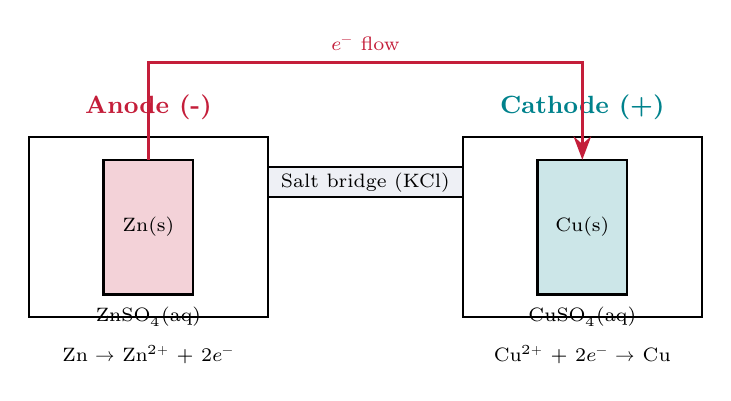
\begin{tikzpicture}[scale=0.95, node distance=0.3cm and 0.5cm,
  sblock/.style={rectangle, draw=myteal, fill=hdrteal, text width=2.0cm,
    align=center, minimum height=1.0cm, font=\small, rounded corners=3pt}]
  % Anode beaker
  \draw[thick] (0,0) rectangle (3.2,2.4);
  \node[font=\small\bfseries, color=myred] at (1.6,2.8) {Anode (-)};
  \draw[fill=myred!20, thick] (1.0,0.3) rectangle (2.2,2.1);
  \node[font=\scriptsize] at (1.6,1.2) {Zn(s)};
  \node[font=\scriptsize] at (1.6,0.0) {ZnSO$_4$(aq)};
  % Cathode beaker
  \draw[thick] (5.8,0) rectangle (9.0,2.4);
  \node[font=\small\bfseries, color=myteal] at (7.4,2.8) {Cathode (+)};
  \draw[fill=myteal!20, thick] (6.8,0.3) rectangle (8.0,2.1);
  \node[font=\scriptsize] at (7.4,1.2) {Cu(s)};
  \node[font=\scriptsize] at (7.4,0.0) {CuSO$_4$(aq)};
  % Salt bridge
  \draw[fill=hdrgray, thick] (3.2,1.6) rectangle (5.8,2.0);
  \node[font=\scriptsize] at (4.5,1.8) {Salt bridge (KCl)};
  % Electron flow (wire)
  \draw[redarrow, very thick] (1.6,2.1) -- (1.6,3.4) -- (7.4,3.4) -- (7.4,2.1);
  \node[font=\scriptsize, color=myred] at (4.5,3.65) {$e^-$ flow};
  % Half-reactions
  \node[font=\scriptsize, align=center] at (1.6,-0.5) {Zn $\to$ Zn$^{2+}$ + 2$e^-$};
  \node[font=\scriptsize, align=center] at (7.4,-0.5) {Cu$^{2+}$ + 2$e^-$ $\to$ Cu};
\end{tikzpicture}
\end{tcolorbox}

\subsection{Relationship Between \texorpdfstring{$\Delta G$}{Delta G} and Cell EMF}
\begin{tcolorbox}[formulabox, title={Free Energy and EMF}]
\[
\Delta G = -nFE, \qquad \Delta G^\circ = -nFE^\circ
\]
$n$ = number of electrons transferred; $F = 96485\ \mathrm{C\,mol^{-1}}$ (Faraday constant).\\
Combining with $\Delta G^\circ = -RT\ln K$:
\[
E^\circ = \frac{RT}{nF}\ln K = \frac{0.0257}{n}\ln K = \frac{0.0591}{n}\log K \quad (298\ \mathrm{K})
\]
\end{tcolorbox}

\subsection{Derivation of the Nernst Equation}
Starting from $\Delta G = \Delta G^\circ + RT\ln Q$ and substituting $\Delta G = -nFE$ and $\Delta G^\circ = -nFE^\circ$:
\[
-nFE = -nFE^\circ + RT\ln Q
\]
Dividing by $-nF$:

\begin{tcolorbox}[formulabox, title={Nernst Equation}]
\[
E = E^\circ - \frac{RT}{nF}\ln Q = E^\circ - \frac{0.0591}{n}\log Q \quad (298\ \mathrm{K})
\]
At equilibrium, $E = 0$ and $Q = K$, confirming $E^\circ = (0.0591/n)\log K$.
\end{tcolorbox}

\begin{tcolorbox}[examplebox, title={Solved Example: Daniell Cell EMF via Nernst}]
Zn/Cu cell: $E^\circ_{\mathrm{cell}} = 0.34 - (-0.76) = 1.10\ \mathrm{V}$, $n=2$.
If $[\mathrm{Zn^{2+}}] = 0.10\ \mathrm{M}$ and $[\mathrm{Cu^{2+}}] = 2.0\ \mathrm{M}$:
\[
Q = \frac{[\mathrm{Zn^{2+}}]}{[\mathrm{Cu^{2+}}]} = \frac{0.10}{2.0} = 0.050
\]
\[
E = 1.10 - \frac{0.0591}{2}\log(0.050) = 1.10 - 0.02955\times(-1.301) = 1.10 + 0.038 = 1.138\ \mathrm{V}
\]
Lower $[\mathrm{Zn^{2+}}]$ and higher $[\mathrm{Cu^{2+}}]$ increases the driving force above the standard value.
\end{tcolorbox}

\begin{tcolorbox}[examplebox, title={Solved Example: Equilibrium Constant from \texorpdfstring{$E^\circ$}{E0}}]
For the Daniell cell ($E^\circ = 1.10\ \mathrm{V}$, $n=2$):
\[
\log K = \frac{n\,E^\circ}{0.0591} = \frac{2\times1.10}{0.0591} = 37.23
\]
\[
K = 10^{37.23} \approx 1.7\times10^{37}
\]
An enormous $K$ confirms the reaction is essentially complete under standard conditions.
\end{tcolorbox}

\subsection{Concentration Cell}
A concentration cell uses the same electrode material in solutions of different concentrations. The EMF arises purely from the concentration difference.

\begin{tcolorbox}[formulabox, title={Concentration Cell EMF}]
\[
E = \frac{0.0591}{n}\log\frac{C_{\mathrm{high}}}{C_{\mathrm{low}}}
\]
At equal concentrations $E = 0$; the cell drives ions from high to low concentration.
\end{tcolorbox}

\subsection{Cell Notation and Standard Cell Notation}
Cells are written with the anode on the left and cathode on the right, separated by a double vertical line (salt bridge):
\[
\mathrm{Zn(s)}\;|\;\mathrm{Zn^{2+}(aq)}\;\|\;\mathrm{Cu^{2+}(aq)}\;|\;\mathrm{Cu(s)}
\]
Single vertical line $|$ = phase boundary; double $\|$ = salt bridge.\\
$E^\circ_{\mathrm{cell}} = E^\circ(\text{right half-cell}) - E^\circ(\text{left half-cell}) = 0.34 - (-0.76) = 1.10\ \mathrm{V}$.

\subsection{Fuel Cells}
A fuel cell is a galvanic device that converts the chemical energy of a fuel (usually H$_2$) directly to electricity without combustion.

\begin{tcolorbox}[formulabox, title={Hydrogen--Oxygen Fuel Cell Reactions}]
\textbf{Anode (alkaline medium):}\quad $\mathrm{2H_2 + 4OH^- \to 4H_2O + 4e^-}$\\
\textbf{Cathode:}\quad $\mathrm{O_2 + 2H_2O + 4e^- \to 4OH^-}$\\
\textbf{Overall:}\quad $\mathrm{2H_2 + O_2 \to 2H_2O}$,\quad $\Delta G^\circ = -474\ \mathrm{kJ\,mol^{-1}}$,\quad $E^\circ = 1.23\ \mathrm{V}$
\end{tcolorbox}

\textbf{Advantages of fuel cells over heat engines:}
\begin{itemize}[leftmargin=*, itemsep=1pt, topsep=2pt]
  \item Efficiency not limited by Carnot efficiency ($\eta_{\mathrm{max}} = 1-T_c/T_h$); can exceed 60\%.
  \item No moving parts in the electrochemical stack.
  \item Zero local emissions (H$_2$-O$_2$ cell produces only water).
  \item Used in spacecraft, buses, and stationary power plants.
\end{itemize}

\begin{tcolorbox}[exambox, title={Exam Points (Section 4)}]
\begin{itemize}[leftmargin=*, itemsep=2pt, topsep=2pt]
  \item $E^\circ_{\mathrm{cell}} = E^\circ_{\mathrm{cathode}} - E^\circ_{\mathrm{anode}}$; higher $E^\circ$ is cathode.
  \item $\Delta G = -nFE$; $\Delta G < 0$ when $E > 0$ (spontaneous cell).
  \item Derive Nernst from $\Delta G = \Delta G^\circ + RT\ln Q$.
  \item $\log K = n E^\circ / 0.0591$ at 298 K.
  \item Concentration cell: EMF from $\log(C_{\mathrm{high}}/C_{\mathrm{low}})$; same electrodes.
\end{itemize}
\end{tcolorbox}

% ===============================================================================
\section{Acid--Base, Redox, and Solubility Equilibria}
% ===============================================================================

\begin{tcolorbox}[defbox]
Three categories of aqueous equilibria are central to engineering chemistry: (i) acid--base equilibria (proton transfer), (ii) redox equilibria (electron transfer), and (iii) solubility equilibria (precipitation). All three are governed by $\Delta G^\circ = -RT\ln K$.
\end{tcolorbox}

\subsection{Br\o{}nsted--Lowry Acid--Base Theory}
\begin{tcolorbox}[defbox]
A \textbf{Br\o{}nsted--Lowry acid} donates a proton; a \textbf{base} accepts one. Every acid has a conjugate base (formed after proton loss) and every base has a conjugate acid. This theory covers aqueous and non-aqueous systems, unlike Arrhenius theory.
\end{tcolorbox}

\textbf{Water autoionisation:} $\mathrm{H_2O + H_2O \rightleftharpoons H_3O^+ + OH^-}$; $K_w = [\mathrm{H_3O^+}][\mathrm{OH^-}] = 1.0\times10^{-14}$ at 298 K.\\
$\mathrm{pH} + \mathrm{pOH} = 14$ at 298 K.

\subsection{Weak Acid Equilibrium and pH Derivation}
For a weak acid HA in water:
\[
\mathrm{HA} \rightleftharpoons \mathrm{H^+} + \mathrm{A^-}, \qquad K_a = \frac{[\mathrm{H^+}][\mathrm{A^-}]}{[\mathrm{HA}]}
\]
If initial concentration is $C$ and degree of dissociation $\alpha \ll 1$:
\[
[\mathrm{H^+}] = \sqrt{K_a C}, \qquad \mathrm{pH} = \tfrac{1}{2}(\mathrm{p}K_a - \log C)
\]

\begin{tcolorbox}[examplebox, title={Solved Example: pH of Acetic Acid}]
$0.10\ \mathrm{M}$ acetic acid, $K_a = 1.8\times10^{-5}$:
\[
[\mathrm{H^+}] = \sqrt{1.8\times10^{-5}\times0.10} = \sqrt{1.8\times10^{-6}} = 1.34\times10^{-3}\ \mathrm{M}
\]
\[
\mathrm{pH} = -\log(1.34\times10^{-3}) = 2.87
\]
Verify with formula: $\mathrm{pH} = \tfrac12(4.74 - (-1)) = 2.87$. \checkmark
\end{tcolorbox}

\subsection{Henderson--Hasselbalch Equation and Buffers}
A buffer solution resists pH change. It consists of a weak acid and its conjugate base (or weak base and conjugate acid).

\begin{tcolorbox}[formulabox, title={Henderson--Hasselbalch Equation}]
\[
\mathrm{pH} = \mathrm{p}K_a + \log\frac{[\mathrm{A^-}]}{[\mathrm{HA}]} = \mathrm{p}K_a + \log\frac{[\text{salt}]}{[\text{acid}]}
\]
\textbf{Derivation:} Take $-\log$ of $K_a = [\mathrm{H^+}][\mathrm{A^-}]/[\mathrm{HA}]$: $\mathrm{pK_a} = \mathrm{pH} - \log([\mathrm{A^-}]/[\mathrm{HA}])$; rearrange.\\
Buffer capacity is maximum when $[\mathrm{A^-}] = [\mathrm{HA}]$, i.e.\ $\mathrm{pH} = \mathrm{p}K_a$.
\end{tcolorbox}

\begin{tcolorbox}[examplebox, title={Solved Example: Buffer pH and Its Change on Adding Acid}]
Acetate buffer: $[\mathrm{CH_3COOH}] = 0.20\ \mathrm{M}$, $[\mathrm{CH_3COONa}] = 0.30\ \mathrm{M}$, $\mathrm{p}K_a = 4.74$:
\[
\mathrm{pH} = 4.74 + \log\frac{0.30}{0.20} = 4.74 + 0.18 = 4.92
\]
Adding $0.01\ \mathrm{mol}$ HCl to 1 L: acid consumes $0.01\ \mathrm{mol}$ of $\mathrm{CH_3COO^-}$:
\[
[\mathrm{A^-}] = 0.29\ \mathrm{M},\quad [\mathrm{HA}] = 0.21\ \mathrm{M},\quad
\mathrm{pH} = 4.74 + \log\frac{0.29}{0.21} = 4.74 + 0.14 = 4.88
\]
pH changed by only $0.04$ despite adding strong acid --- the buffer works.
\end{tcolorbox}

\subsection{Biological Importance of Buffers}
\begin{itemize}[leftmargin=*, itemsep=2pt, topsep=2pt]
  \item Blood pH ($7.35$--$7.45$) maintained by the bicarbonate buffer: $\mathrm{H_2CO_3}/\mathrm{HCO_3^-}$ ($\mathrm{p}K_a = 6.35$) reinforced by respiratory control of $\mathrm{CO_2}$.
  \item Intracellular pH maintained by phosphate buffer ($\mathrm{H_2PO_4^-}/\mathrm{HPO_4^{2-}}$, $\mathrm{p}K_a = 7.2$).
  \item Industrial buffers: electroplating baths, pharmaceutical formulations.
\end{itemize}

\subsection{Lewis Acid--Base Theory}
\begin{tcolorbox}[defbox]
\textbf{Lewis acid:} Electron-pair acceptor. \textbf{Lewis base:} Electron-pair donor. This is the broadest acid--base definition and covers reactions without proton transfer, such as complex-ion formation.
\end{tcolorbox}

\begin{tabularx}{\linewidth}{|B{2.4cm}|Y|Y|}
\hline
\textbf{Concept} & \textbf{Arrhenius} & \textbf{Brønsted--Lowry} and \textbf{Lewis} \\
\hline
Acid & Produces H$^+$ in water & H$^+$ donor / electron-pair acceptor \\
\hline
Base & Produces OH$^-$ in water & H$^+$ acceptor / electron-pair donor \\
\hline
Scope & Aqueous only & Aqueous and non-aqueous \\
\hline
Example & HCl, NaOH & NH$_3$: Lewis base; BF$_3$: Lewis acid \\
\hline
\end{tabularx}

\textbf{Lewis examples:} $\mathrm{BF_3 + NH_3 \to F_3B{:}NH_3}$ (adduct); metal-ligand complex formation $\mathrm{Cu^{2+} + 4NH_3 \to [Cu(NH_3)_4]^{2+}}$ (Cu$^{2+}$ = Lewis acid, NH$_3$ = Lewis base).

\subsection{Redox Equilibria and Disproportionation}
\begin{tcolorbox}[defbox]
\textbf{Disproportionation:} A reaction in which the same element is simultaneously oxidised and reduced. Example: $\mathrm{2Cu^+(aq) \to Cu^{2+}(aq) + Cu(s)}$.
\end{tcolorbox}

\textbf{Predicting feasibility of redox reactions using $E^\circ$:}
\begin{itemize}[leftmargin=*, itemsep=1pt, topsep=2pt]
  \item $E^\circ_{\mathrm{cell}} > 0$ ($\Delta G^\circ < 0$): reaction spontaneous.
  \item $E^\circ_{\mathrm{cell}} < 0$: non-spontaneous in the written direction.
\end{itemize}

\textbf{Disproportionation of Cu$^+$:}
\begin{align*}
\text{Cathode:}&\quad \mathrm{Cu^+(aq) + e^- \to Cu(s)},\quad E^\circ = +0.52\ \mathrm{V}\\
\text{Anode:}&\quad \mathrm{Cu(s) \to Cu^+(aq) + e^-},\quad E^\circ = -0.34\ \mathrm{V}\quad\text{wait...}
\end{align*}
Actually using the two half-reactions:
$\mathrm{Cu^+ + e^- \to Cu}$ ($+0.52\ \mathrm{V}$) and $\mathrm{Cu^{2+} + e^- \to Cu^+}$ ($+0.16\ \mathrm{V}$).
$E^\circ_{\mathrm{cell}} = 0.52 - 0.16 = +0.36\ \mathrm{V} > 0$, so Cu$^+$ is unstable to disproportionation in aqueous solution.

\subsection{Solubility Product \texorpdfstring{$K_{sp}$}{Ksp}}
For a sparingly soluble salt $\mathrm{M}_m\mathrm{X}_n(s) \rightleftharpoons m\mathrm{M}^{n+} + n\mathrm{X}^{m-}$:

\begin{tcolorbox}[formulabox, title={Solubility Product}]
\[
K_{sp} = [\mathrm{M}^{n+}]^m[\mathrm{X}^{m-}]^n
\]
\textbf{Ionic product (IP):} $[\mathrm{M}^{n+}]^m[\mathrm{X}^{m-}]^n$ using current concentrations.
\begin{itemize}[leftmargin=*, itemsep=1pt, topsep=2pt]
  \item IP $< K_{sp}$: unsaturated, no precipitation.
  \item IP $= K_{sp}$: saturated, equilibrium.
  \item IP $> K_{sp}$: supersaturated, precipitation occurs.
\end{itemize}
\end{tcolorbox}

\begin{tcolorbox}[examplebox, title={Solved Example: Solubility from \texorpdfstring{$K_{sp}$}{Ksp}}]
$K_{sp}(\mathrm{BaSO_4}) = 1.1\times10^{-10}$ at 298 K. Find molar solubility $s$ in pure water.
\[
\mathrm{BaSO_4 \rightleftharpoons Ba^{2+} + SO_4^{2-}},\quad K_{sp} = s\cdot s = s^2
\]
\[
s = \sqrt{1.1\times10^{-10}} = 1.05\times10^{-5}\ \mathrm{mol\,L^{-1}}
\]
In $0.10\ \mathrm{M}\ \mathrm{Na_2SO_4}$ (common ion effect):
\[
K_{sp} = s\cdot(0.10 + s) \approx 0.10\,s \quad\Rightarrow\quad s = \frac{1.1\times10^{-10}}{0.10} = 1.1\times10^{-9}\ \mathrm{mol\,L^{-1}}
\]
Common ion reduces solubility by a factor of $\sim 10^4$.
\end{tcolorbox}

\begin{tcolorbox}[exambox, title={Exam Points (Section 5)}]
\begin{itemize}[leftmargin=*, itemsep=2pt, topsep=2pt]
  \item Brønsted--Lowry: acid = proton donor; base = proton acceptor.
  \item $K_a \times K_b = K_w = 10^{-14}$; $\mathrm{pH + pOH = 14}$ at 298 K.
  \item Weak acid pH: $\mathrm{pH} = \tfrac12(\mathrm{pK_a} - \log C)$.
  \item Henderson--Hasselbalch: $\mathrm{pH} = \mathrm{pK_a} + \log([\mathrm{A^-}]/[\mathrm{HA}])$; buffer works near $\mathrm{pK_a}$.
  \item $K_{sp}$ solubility product: IP $> K_{sp}$ gives precipitation; common ion reduces solubility.
\end{itemize}
\end{tcolorbox}

% ===============================================================================
\section{Water Chemistry and Corrosion}
% ===============================================================================

\begin{tcolorbox}[defbox]
\textbf{Water chemistry} deals with the dissolved ions, gases, and organic matter in natural and industrial water, especially as they affect engineering systems. \textbf{Corrosion} is the electrochemical deterioration of metals driven by a spontaneous redox reaction ($\Delta G < 0$). Both topics are directly governed by the free-energy and equilibrium principles of this module.
\end{tcolorbox}

\subsection{Hardness of Water}
Hard water contains dissolved $\mathrm{Ca^{2+}}$ and $\mathrm{Mg^{2+}}$ ions, primarily as bicarbonates, chlorides, and sulphates. Hardness is expressed in parts per million (ppm) as equivalent $\mathrm{CaCO_3}$.

\begin{tcolorbox}[formulabox, title={Hardness in ppm as \texorpdfstring{$\mathrm{CaCO_3}$}{CaCO3} Equivalent}]
\[
\text{Hardness (ppm)} = \frac{\text{mass of salt (g)}}{\text{volume of water (L)}}\times\frac{M(\mathrm{CaCO_3})}{M(\text{salt})}\times1000
\]
Or: $\text{ppm} = \frac{w_{\mathrm{CaCO_3\text{-equiv}}}}{V_{\text{water}}}\times10^6$.\\
Soft water: $<75\ \mathrm{ppm}$. Moderately hard: $75$--$150\ \mathrm{ppm}$. Hard: $>150\ \mathrm{ppm}$.
\end{tcolorbox}

\begin{tabularx}{\linewidth}{|B{2.8cm}|Y|Y|}
\hline
\textbf{Type} & \textbf{Cause} & \textbf{Removal} \\
\hline
Temporary hardness & $\mathrm{Ca(HCO_3)_2}$, $\mathrm{Mg(HCO_3)_2}$ & Boiling, lime addition \\
\hline
Permanent hardness & $\mathrm{CaCl_2}$, $\mathrm{MgCl_2}$, $\mathrm{CaSO_4}$, $\mathrm{MgSO_4}$ & Lime-soda, zeolite, ion exchange \\
\hline
\end{tabularx}

\subsection{Boiler Troubles}
Hard water in steam boilers causes multiple engineering problems.

\begin{tabularx}{\linewidth}{|B{2.6cm}|Y|Y|Y|}
\hline
\textbf{Problem} & \textbf{Cause} & \textbf{Effect} & \textbf{Remedy} \\
\hline
Scale formation & Deposition of $\mathrm{CaCO_3}$, $\mathrm{Mg(OH)_2}$, $\mathrm{CaSO_4}$ & Reduced heat transfer; tube overheating and bursting & Softening; acid descaling \\
\hline
Sludge formation & Loose precipitates of $\mathrm{MgCO_3}$, $\mathrm{MgCl_2}$ & Chokes pipes; reduces efficiency & Blow-down of boiler \\
\hline
Priming & High dissolved solids, oil, or organic impurities & Wet steam carries water droplets; turbine erosion & Filtration; demineralisation \\
\hline
Foaming & Organic impurities or oil stabilise steam bubbles & Irregular operation; carryover & Anti-foam chemicals \\
\hline
Caustic embrittlement & Concentrated NaOH in stressed joints/cracks & Metal grain-boundary cracking and failure & Neutralise with sodium sulphate \\
\hline
\end{tabularx}

\subsection{Water Softening Methods}
\begin{tabularx}{\linewidth}{|B{2.6cm}|Y|Y|}
\hline
\textbf{Method} & \textbf{Principle} & \textbf{Notes} \\
\hline
Lime--soda process & Add $\mathrm{Ca(OH)_2}$ and $\mathrm{Na_2CO_3}$; precipitate $\mathrm{CaCO_3}$ and $\mathrm{Mg(OH)_2}$ & Cheap; used for large volumes; produces sludge \\
\hline
Zeolite / ion exchange & $\mathrm{Ca^{2+}}$ and $\mathrm{Mg^{2+}}$ exchanged for $\mathrm{Na^+}$ on zeolite resin & Portable; regenerated with NaCl; does not reduce TDS \\
\hline
Demineralisation & Cation exchanger (H$^+$ form) + anion exchanger (OH$^-$ form) & Removes all ions; produces ultra-pure water \\
\hline
Reverse osmosis & Applied pressure forces water through semi-permeable membrane & Removes ions, bacteria, organics \\
\hline
\end{tabularx}

\subsection{Electrochemical Theory of Corrosion}
Corrosion of iron in neutral or acidic water is an electrochemical process requiring an anode (oxidation), a cathode (reduction), an electrolyte, and a metallic conductor.

\begin{tcolorbox}[formulabox, title={Iron Corrosion Half-Reactions}]
\textbf{Anodic reaction (oxidation):}
\[
\mathrm{Fe(s) \to Fe^{2+}(aq) + 2e^-}, \qquad E^\circ = +0.44\ \mathrm{V\ (vs\ SHE)}
\]
\textbf{Cathodic reaction (oxygen reduction, neutral/alkaline):}
\[
\mathrm{O_2(g) + 2H_2O(l) + 4e^- \to 4OH^-(aq)}, \qquad E^\circ = +0.40\ \mathrm{V}
\]
\textbf{Overall:}
\[
\mathrm{2Fe + O_2 + 2H_2O \to 2Fe(OH)_2}
\]
Further air oxidation: $\mathrm{4Fe(OH)_2 + O_2 + 2H_2O \to 4Fe(OH)_3}$ $\to$ rust (hydrated $\mathrm{Fe_2O_3}$).
\end{tcolorbox}

\begin{tcolorbox}[tikzbox, title={Differential Aeration Corrosion Cell}]
\centering
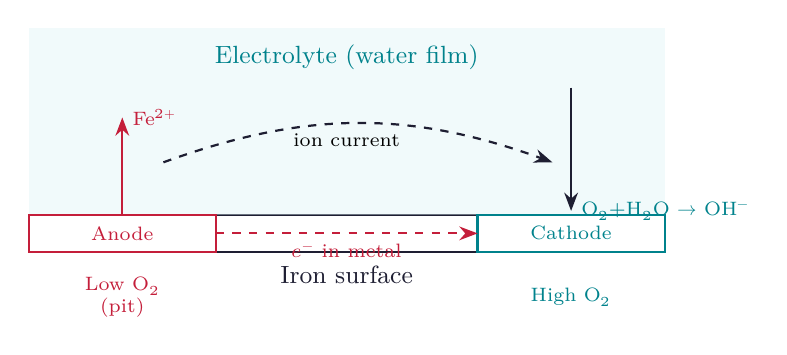
\begin{tikzpicture}[scale=0.95]
  % Iron surface
  \draw[thick, mydark] (0,0) rectangle (8.5,0.5);
  \node[font=\small, color=mydark] at (4.25,-0.3) {Iron surface};
  % Electrolyte above
  \fill[hdrteal, opacity=0.4] (0,0.5) rectangle (8.5,3.0);
  \node[font=\small, color=myteal] at (4.25,2.6) {Electrolyte (water film)};
  % Anode region (left, low O2)
  \draw[thick, myred] (0,0) rectangle (2.5,0.5);
  \node[font=\scriptsize, color=myred] at (1.25,0.25) {Anode};
  \node[font=\scriptsize, color=myred, align=center] at (1.25,-0.6) {Low O$_2$\\(pit)};
  \draw[redarrow] (1.25,0.5) -- (1.25,1.8) node[right, font=\scriptsize, color=myred] {Fe$^{2+}$};
  % Cathode region (right, high O2)
  \draw[thick, myteal] (6.0,0) rectangle (8.5,0.5);
  \node[font=\scriptsize, color=myteal] at (7.25,0.25) {Cathode};
  \node[font=\scriptsize, color=myteal, align=center] at (7.25,-0.6) {High O$_2$};
  \draw[arrow] (7.25,2.2) -- (7.25,0.55) node[right, font=\scriptsize, color=myteal] {O$_2$+H$_2$O $\to$ OH$^-$};
  % Electron flow in metal
  \draw[redarrow, dashed] (2.5,0.25) -- (6.0,0.25) node[midway, below, font=\scriptsize] {$e^-$ in metal};
  % Ion flow in electrolyte
  \draw[arrow, dashed] (1.8,1.2) to[bend left=20] (7.0,1.2);
  \node[font=\scriptsize] at (4.25,1.5) {ion current};
\end{tikzpicture}
\end{tcolorbox}

\textbf{Factors accelerating corrosion:} Higher temperature, lower pH, higher dissolved $\mathrm{O_2}$, electrolyte concentration, stressed metal, galvanic coupling with nobler metal.

\subsection{Dissolved Oxygen, BOD, and COD}
These three parameters are standard measures of water quality and appear in MAKAUT water-chemistry questions.

\begin{tcolorbox}[defbox]
\textbf{Dissolved Oxygen (DO):} Oxygen dissolved in water; typical freshwater has $8$--$14\ \mathrm{mg\,L^{-1}}$. Falls below $5\ \mathrm{mg\,L^{-1}}$ in polluted water, harming aquatic life.\\
\textbf{BOD (Biochemical Oxygen Demand):} Oxygen consumed by microorganisms to decompose organic matter in 5 days at 20$^\circ$C (BOD$_5$). High BOD = heavy organic pollution.\\
\textbf{COD (Chemical Oxygen Demand):} Oxygen equivalent needed to oxidise all organic and inorganic matter chemically (with K$_2$Cr$_2$O$_7$ as oxidant). COD $\geq$ BOD always.
\end{tcolorbox}

\begin{tabularx}{\linewidth}{|B{2.6cm}|Y|Y|}
\hline
\textbf{Parameter} & \textbf{Clean water} & \textbf{Polluted water} \\
\hline
DO (mg/L) & 8--14 & $<$5 (danger zone) \\
\hline
BOD (mg/L) & $<$1--2 & $>$100 (sewage $\sim$ 300) \\
\hline
COD (mg/L) & $<$10 & $>$150 \\
\hline
\end{tabularx}

\subsection{Passivation}
\begin{tcolorbox}[defbox]
\textbf{Passivation:} Formation of a thin, dense, adherent oxide film on a metal surface that blocks further corrosion. The film is self-healing when scratched in air. Examples: Al forms Al$_2$O$_3$ (3 nm thick), stainless steel forms Cr$_2$O$_3$, Ti forms TiO$_2$.
\end{tcolorbox}

Passivation requires the oxide to be: (i) insoluble in the corrosive medium, (ii) adherent (not flaking), (iii) dense enough to prevent ion/electron diffusion.\\
\textbf{Concentration of HNO$_3$ and passivation of iron:} Dilute HNO$_3$ dissolves iron (active dissolution); concentrated HNO$_3$ passivates iron by forming a dense Fe$_3$O$_4$/Fe$_2$O$_3$ surface layer — a standard MAKAUT viva question.

\subsection{Corrosion Prevention}
\begin{tabularx}{\linewidth}{|B{2.8cm}|Y|Y|}
\hline
\textbf{Method} & \textbf{Principle} & \textbf{Example} \\
\hline
Barrier coatings & Physically isolate metal from electrolyte & Paint, polymer coating, oxide passivation \\
\hline
Galvanisation & Sacrificial zinc oxidises preferentially to iron; even at scratches Zn protects Fe & Zn-coated steel sheets \\
\hline
Sacrificial anode & More active metal (Mg, Zn, Al) connected as anode; made to corrode instead of structure & Ship hulls, buried pipelines \\
\hline
Impressed current & External DC supply makes structure cathodic; no net oxidation & Underground pipelines, bridges \\
\hline
Alloying & Cr$_2$O$_3$ passive film on stainless steel blocks O$_2$/H$_2$O access & Stainless steel ($>11\%$ Cr) \\
\hline
Inhibitors & Adsorb on metal surface, reduce anodic/cathodic reaction rate & Boiler treatment chemicals \\
\hline
\end{tabularx}

\textbf{Sacrificial anode vs impressed current:}\par\noindent
\begin{tabularx}{\linewidth}{|B{3.0cm}|Y|Y|}
\hline
\textbf{Feature} & \textbf{Sacrificial anode} & \textbf{Impressed current} \\
\hline
Power source & None (galvanic cell) & External DC rectifier \\
\hline
Anode material & Mg, Zn, or Al alloy & Inert (platinised Ti, graphite) \\
\hline
Maintenance & Replace anode periodically & Monitor current; less material cost \\
\hline
Suitable for & Small isolated structures & Large structures, long pipelines \\
\hline
\end{tabularx}

\begin{tcolorbox}[exambox, title={Exam Points (Section 6)}]
\begin{itemize}[leftmargin=*, itemsep=2pt, topsep=2pt]
  \item Hardness ppm = mass of CaCO$_3$ equivalent per litre $\times 10^6$.
  \item Temporary hardness: bicarbonates; removed by boiling. Permanent: chlorides/sulphates; need chemical treatment.
  \item Boiler scale: CaCO$_3$ and CaSO$_4$ deposits reduce heat transfer and cause overheating.
  \item Corrosion: Fe is anode (oxidised); O$_2$/H$^+$ cathodic reduction drives current.
  \item Sacrificial anode: Zn/Mg corrodes preferentially protecting Fe.
  \item Stainless steel: passive Cr$_2$O$_3$ film blocks electrolyte contact.
\end{itemize}
\end{tcolorbox}

% ===============================================================================
\section{Ellingham Diagrams and Free Energy in Metallurgy}
% ===============================================================================

\begin{tcolorbox}[defbox]
An \textbf{Ellingham diagram} plots the standard Gibbs free energy of oxide formation ($\Delta G^\circ = \Delta H^\circ - T\Delta S^\circ$) against temperature for a series of metal--oxygen reactions. It is the primary tool for selecting a reducing agent in pyrometallurgy and for predicting the stability of oxides.
\end{tcolorbox}

\subsection{Construction and Interpretation}
For the standard reaction written as oxidation of 1 mol O$_2$:
\[
\tfrac{2x}{y}\mathrm{M}(s) + \mathrm{O_2}(g) \to \tfrac{2}{y}\mathrm{M_xO_y}(s)
\]
$\Delta G^\circ = \Delta H^\circ - T\Delta S^\circ$.

\begin{itemize}[leftmargin=*, itemsep=2pt, topsep=2pt]
  \item Mostly straight lines because $\Delta H^\circ$ and $\Delta S^\circ$ are nearly independent of $T$.
  \item Slope $= -\Delta S^\circ_{\mathrm{rxn}}$. Consuming one mole O$_2$(g) makes $\Delta S^\circ < 0$ (gas disappears), so slope is \emph{positive} (line rises with $T$) for most metal oxidations.
  \item \textbf{Exceptions:} $\mathrm{C + O_2 \to CO_2}$: $\Delta n_{\mathrm{gas}} = 0$, nearly horizontal. $\mathrm{2C + O_2 \to 2CO}$: $\Delta n_{\mathrm{gas}} = +1$, slope is \emph{negative} (line falls with $T$).
  \item \textbf{Slope changes:} A kink (sudden change in slope) occurs at the melting or boiling point of the metal because $\Delta S^\circ$ changes (latent heat term).
\end{itemize}

\begin{tcolorbox}[tikzbox, title={Schematic Ellingham Diagram (three key lines)}]
\centering
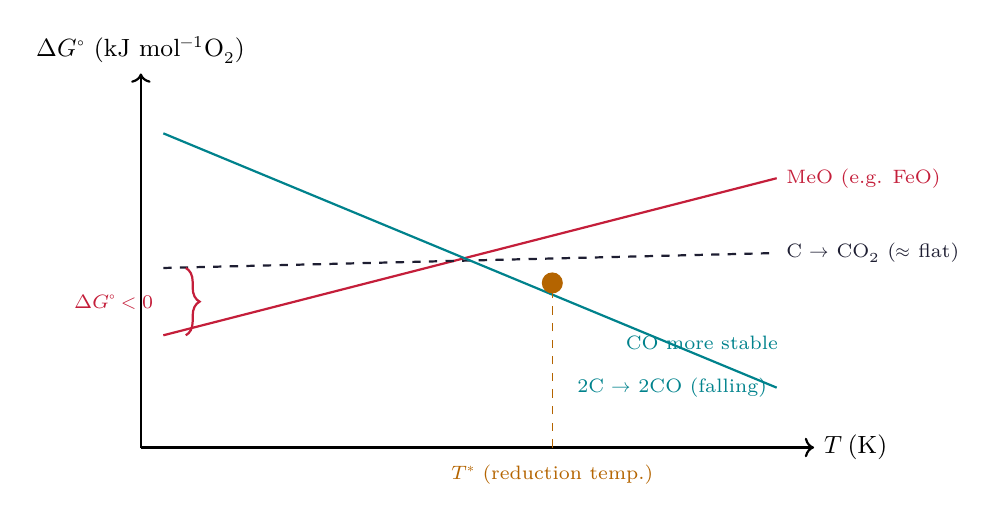
\begin{tikzpicture}[scale=0.95]
  \draw[->, thick] (0,0) -- (9.0,0) node[right, font=\small] {$T$ (K)};
  \draw[->, thick] (0,0) -- (0,5.0) node[above, font=\small] {$\Delta G^\circ$ (kJ mol$^{-1}$O$_2$)};
  % Metal oxide (rising line, e.g. Fe2O3)
  \draw[myred, thick] (0.3,1.5) -- (8.5,3.6);
  \node[myred, font=\scriptsize, anchor=west] at (8.5,3.6) {MeO (e.g. FeO)};
  % C -> CO2 (nearly horizontal)
  \draw[mydark, thick, dashed] (0.3,2.4) -- (8.5,2.6);
  \node[mydark, font=\scriptsize, anchor=west] at (8.5,2.6) {C $\to$ CO$_2$ ($\approx$ flat)};
  % 2C -> 2CO (falling line, crosses MeO at T*)
  \draw[myteal, thick] (0.3,4.2) -- (8.5,0.8);
  \node[myteal, font=\scriptsize, anchor=east] at (8.5,0.8) {2C $\to$ 2CO (falling)};
  % Crossover
  \fill[myamber] (5.5,2.2) circle (4pt);
  \draw[dashed, myamber] (5.5,0) -- (5.5,2.2);
  \node[myamber, font=\scriptsize, anchor=north] at (5.5,-0.1) {$T^*$ (reduction temp.)};
  % Arrow
  \draw[decorate, decoration={brace, amplitude=5pt}, myred, thick]
       (0.6,2.4) -- (0.6,1.5) node[midway, left=8pt, font=\scriptsize, color=myred] {$\Delta G^\circ < 0$};
  \node[font=\scriptsize, color=myteal] at (7.5,1.4) {CO more stable};
\end{tikzpicture}
\end{tcolorbox}

\subsection{Rules for Selecting a Reducing Agent}
\begin{tcolorbox}[formulabox, title={Ellingham Selection Rule}]
A metal oxide $\mathrm{MO}$ can be reduced by a reducing agent $\mathrm{R}$ at temperature $T$ if the $\Delta G^\circ$ line of $\mathrm{R+O_2 \to RO_2}$ lies \emph{below} the $\Delta G^\circ$ line of $\mathrm{2M+O_2 \to 2MO}$ at that temperature.

The overall reaction $\mathrm{MO + R \to M + RO}$ has $\Delta G^\circ = \Delta G^\circ(\mathrm{MO\;line}) - \Delta G^\circ(\mathrm{RO\;line}) > 0$ … wait --- actually \emph{subtract lower from upper}: net $\Delta G^\circ < 0$ only when the reducing agent's line is lower.

In short: \textbf{the oxide whose line is lower is more stable; its metal is harder to reduce. Use a reducing agent whose line is below the ore's line at the operating temperature.}
\end{tcolorbox}

\subsection{Carbon as a Reducing Agent: The Blast Furnace}
Carbon has two Ellingham lines: $\mathrm{C + O_2 \to CO_2}$ (flat) and $\mathrm{2C + O_2 \to 2CO}$ (descending). Above $\sim 700^\circ\mathrm{C}$ the CO line lies below most metal oxide lines, making carbon (via CO) an effective industrial reducing agent.

\textbf{Blast furnace reactions:}
\begin{align*}
\mathrm{C + O_2} &\to \mathrm{CO_2} \quad \text{(combustion zone)}\\
\mathrm{CO_2 + C} &\to \mathrm{2CO} \quad \text{(Boudouard reaction)}\\
\mathrm{Fe_2O_3 + 3CO} &\to \mathrm{2Fe + 3CO_2} \quad \text{(reduction zone)}\\
\mathrm{CaCO_3} &\to \mathrm{CaO + CO_2} \quad \text{(flux decomposition)}\\
\mathrm{CaO + SiO_2} &\to \mathrm{CaSiO_3} \quad \text{(slag formation)}
\end{align*}

\subsection{Thermite Reaction: Aluminium Reducing Iron Oxide}
Aluminium sits below iron oxide on the Ellingham diagram at room temperature, so:
\[
\mathrm{Fe_2O_3 + 2Al \to Al_2O_3 + 2Fe}, \qquad \Delta G^\circ \approx -842\ \mathrm{kJ\,mol^{-1}}
\]
The large negative $\Delta G^\circ$ means the reaction is strongly spontaneous and highly exothermic ($\Delta H \approx -847\ \mathrm{kJ\,mol^{-1}}$), producing liquid iron at $\sim 2500\ \mathrm{K}$. Used in rail welding and incendiary applications.

\begin{tcolorbox}[examplebox, title={Solved Example: Reading the Ellingham Diagram}]
\textbf{Problem:} At what minimum temperature can coke (carbon) reduce ZnO?\\
\textbf{Given:} The $\Delta G^\circ$ lines of $\mathrm{2Zn + O_2 \to 2ZnO}$ and $\mathrm{2C + O_2 \to 2CO}$ cross at approximately $T^* = 950^\circ\mathrm{C}$.
\[
\text{Above } 950^\circ\mathrm{C}: \quad \Delta G^\circ(\mathrm{C\to CO}) < \Delta G^\circ(\mathrm{Zn\to ZnO})
\]
\[
\mathrm{ZnO + C \to Zn + CO}, \qquad \Delta G^\circ_{\mathrm{net}} < 0
\]
Industrial zinc smelters operate at $\sim 1000$--$1100^\circ\mathrm{C}$.
\end{tcolorbox}

\subsection{Limitations of Ellingham Diagrams}
\begin{itemize}[leftmargin=*, itemsep=2pt, topsep=2pt]
  \item Assumes pure solid/liquid phases (unit activity); does not account for alloy formation.
  \item Does not give information about reaction rate (kinetics).
  \item Phase changes (melting, boiling) cause kinks but data is not always available for all phases.
  \item Atmospheric composition (partial pressure of O$_2$) affects actual $\Delta G$.
\end{itemize}

\subsection{Industrial Extraction Examples Using Ellingham Diagram}
\begin{tabularx}{\linewidth}{|B{2.4cm}|Y|Y|Y|}
\hline
\textbf{Metal} & \textbf{Ore} & \textbf{Reducing agent at $T$} & \textbf{Typical temperature} \\
\hline
Iron (Fe) & Fe$_2$O$_3$ (haematite) & C (as CO) in blast furnace & $800$--$1600^\circ$C \\
\hline
Copper (Cu) & Cu$_2$S (chalcocite) & Roasting to Cu$_2$O then C or self-reduction & $\sim 1000^\circ$C \\
\hline
Zinc (Zn) & ZnO (from roasting ZnS) & C (as CO/C) & $\sim 1000^\circ$C \\
\hline
Lead (Pb) & PbO (from roasting galena) & C & $\sim 700^\circ$C \\
\hline
Aluminium (Al) & Al$_2$O$_3$ (bauxite) & Electrolysis (too stable for C reduction) & Hall-H\'{e}roult at $960^\circ$C \\
\hline
\end{tabularx}

\textbf{Why aluminium cannot be reduced by carbon from Ellingham:} The Al$_2$O$_3$ line is always below the CO line even at 2000$^\circ$C. The reaction Al$_2$O$_3$ + C $\to$ Al + CO has $\Delta G^\circ > 0$ at all practical temperatures, so electrolysis is used instead.

\begin{tcolorbox}[exambox, title={Exam Points (Section 7)}]
\begin{itemize}[leftmargin=*, itemsep=2pt, topsep=2pt]
  \item Ellingham line slope = $-\Delta S^\circ$; positive (rising) for most metal oxidations; negative for $2\mathrm{C}\to2\mathrm{CO}$.
  \item Reducing agent selection: line below = more stable oxide = better reducing agent.
  \item Blast furnace: C converts to CO via Boudouard reaction; CO reduces Fe$_2$O$_3$ above $\sim700^\circ$C.
  \item Thermite: Al reduces Fe$_2$O$_3$; $\Delta G^\circ \approx -842\ \mathrm{kJ\,mol^{-1}}$.
  \item Kink in a line: phase change (melting/boiling of metal).
\end{itemize}
\end{tcolorbox}

\newpage
\begin{center}
  {\large\bfseries\color{myred} Quick Revision --- Module 4}\\[3pt]
  {\small\color{mydark} Free Energy and Chemical Equilibria $|$ BS-CH101}
\end{center}
\noindent{\color{myred}\rule{\linewidth}{1.2pt}}
\vspace{6pt}

% --- Key Formulas: longtable so it breaks cleanly across pages ---------------
\begin{tcolorbox}[formulabox, breakable, title={Key Formulas at a Glance},
  title after break={\textbf{Key Formulas at a Glance (contd.)}}]
\renewcommand{\arraystretch}{1.55}
\begin{tabularx}{\linewidth}{|B{4.6cm}|Y|}
\hline
\textbf{Formula} & \textbf{Meaning} \\
\hline
$\Delta U = q + w$ & First law: energy conserved. \\
\hline
$\Delta H = \Delta U + \Delta(PV)$ & Enthalpy; at const $P$: $q_P = \Delta H$. \\
\hline
$C_P - C_V = R$ & Ideal gas heat capacity relation. \\
\hline
$\Delta H_{\mathrm{rxn}} = \sum \Delta H_f^\circ(\text{prod}) - \sum \Delta H_f^\circ(\text{react})$ & Hess's law. \\
\hline
$\Delta S = \displaystyle\int \frac{\delta q_{\mathrm{rev}}}{T}$ & Entropy from reversible heat. \\
\hline
$\Delta S_{\mathrm{univ}} = \Delta S_{\mathrm{sys}} + \Delta S_{\mathrm{surr}} \geq 0$ & Second law. \\
\hline
$\Delta G = \Delta H - T\Delta S$ & Gibbs free energy criterion. \\
\hline
$T^* = \Delta H / \Delta S$ & Crossover temperature ($\Delta G = 0$). \\
\hline
\end{tabularx}
\vspace{3pt}
\begin{tabularx}{\linewidth}{|B{4.6cm}|Y|}
\hline
$\left(\displaystyle\frac{\partial(\Delta G/T)}{\partial T}\right)_P = -\displaystyle\frac{\Delta H}{T^2}$ & Gibbs--Helmholtz equation. \\
\hline
$\Delta G = \Delta G^\circ + RT\ln Q$ & Free energy at non-standard conditions. \\
\hline
$\Delta G^\circ = -RT\ln K$ & Standard free energy and equilibrium constant. \\
\hline
$\ln\displaystyle\frac{K_2}{K_1} = -\displaystyle\frac{\Delta H^\circ}{R}\!\left(\displaystyle\frac{1}{T_2}-\displaystyle\frac{1}{T_1}\right)$ & Van't Hoff equation. \\
\hline
$E^\circ_{\mathrm{cell}} = E^\circ_{\mathrm{cathode}} - E^\circ_{\mathrm{anode}}$ & Standard cell EMF. \\
\hline
$\Delta G = -nFE$;\; $\Delta G^\circ = -nFE^\circ$ & Free energy and EMF. \\
\hline
$E = E^\circ - \displaystyle\frac{0.0591}{n}\log Q$ & Nernst equation at 298 K. \\
\hline
$\log K = \displaystyle\frac{n E^\circ}{0.0591}$ & $K$ from standard cell EMF. \\
\hline
\end{tabularx}
\vspace{3pt}
\begin{tabularx}{\linewidth}{|B{4.6cm}|Y|}
\hline
$K_w = [\mathrm{H^+}][\mathrm{OH^-}] = 10^{-14}$ & Water ionic product (298 K). \\
\hline
$\mathrm{pH} = \tfrac12(\mathrm{pK_a} - \log C)$ & pH of weak acid solution. \\
\hline
$\mathrm{pH} = \mathrm{p}K_a + \log\displaystyle\frac{[\mathrm{A^-}]}{[\mathrm{HA}]}$ & Henderson--Hasselbalch (buffer). \\
\hline
$K_{sp} = [\mathrm{M}^{n+}]^m[\mathrm{X}^{m-}]^n$ & Solubility product. \\
\hline
$K_p = K_c\,(RT)^{\Delta n_g}$ & Relationship between $K_p$ and $K_c$. \\
\hline
$w_{\mathrm{rev}} = -nRT\ln(V_2/V_1)$ & Reversible isothermal expansion work. \\
\hline
$\Delta S_{\mathrm{vap}} = \Delta H_{\mathrm{vap}}/T_b$ & Entropy of vaporisation. \\
\hline
$\Delta H_{T_2} = \Delta H_{T_1} + \Delta C_P\,(T_2-T_1)$ & Kirchhoff's equation. \\
\hline
$s = \sqrt{K_{sp}}$ & Molar solubility of 1:1 salt. \\
\hline
\end{tabularx}
\end{tcolorbox}

\begin{tcolorbox}[defbox, title={One-Line Definitions}]
\begin{itemize}[leftmargin=*, itemsep=2pt, topsep=2pt]
  \item \textbf{Internal energy ($U$):} Total kinetic and potential energy of all molecules in a system.
  \item \textbf{Enthalpy ($H$):} $H = U + PV$; heat flow at constant pressure.
  \item \textbf{Heat capacity ($C_P$):} Heat required to raise temperature by 1 K at constant pressure.
  \item \textbf{Hess's law:} Enthalpy change is independent of reaction pathway.
  \item \textbf{Entropy ($S$):} Measure of energy dispersal; $\Delta S_{\mathrm{univ}} > 0$ for spontaneous processes.
  \item \textbf{Third law:} $S = 0$ for a perfect crystal at $T = 0\ \mathrm{K}$.
  \item \textbf{Gibbs free energy ($G$):} $G = H - TS$; $\Delta G < 0$ for spontaneous process at const $T$, $P$.
  \item \textbf{Crossover temperature ($T^*$):} Temperature at which $\Delta G = 0$; $T^* = \Delta H/\Delta S$.
  \item \textbf{Reaction quotient ($Q$):} Ratio of product to reactant activities at current conditions.
  \item \textbf{Equilibrium constant ($K$):} $Q$ at equilibrium; $\Delta G^\circ = -RT\ln K$.
  \item \textbf{Van't Hoff equation:} Describes temperature dependence of $K$; derived from $\Delta G^\circ = \Delta H^\circ - T\Delta S^\circ$.
  \item \textbf{Le Chatelier's principle:} System shifts to partially counteract any imposed change.
  \item \textbf{Standard hydrogen electrode (SHE):} Reference electrode, $E^\circ = 0.000\ \mathrm{V}$.
  \item \textbf{Nernst equation:} $E = E^\circ - (RT/nF)\ln Q$; relates cell potential to concentration.
  \item \textbf{Faraday constant ($F$):} $96485\ \mathrm{C\,mol^{-1}}$; charge per mole of electrons.
  \item \textbf{Concentration cell:} Cell with identical electrodes at different concentrations; EMF from $\log(C_1/C_2)$.
  \item \textbf{Brønsted--Lowry acid:} Proton donor; its conjugate base forms after proton loss.
  \item \textbf{Buffer solution:} Resists pH change; contains weak acid + conjugate base near $\mathrm{pK_a}$.
  \item \textbf{Henderson--Hasselbalch:} $\mathrm{pH} = \mathrm{pK_a} + \log([\mathrm{A^-}]/[\mathrm{HA}])$.
  \item \textbf{Solubility product ($K_{sp}$):} Ion activity product in a saturated solution.
  \item \textbf{Common ion effect:} Adding a common ion suppresses solubility.
  \item \textbf{Temporary hardness:} Due to bicarbonates; removed by boiling.
  \item \textbf{Permanent hardness:} Due to chlorides/sulphates; requires chemical treatment.
  \item \textbf{Scale:} Hard insulating deposit in boilers; reduces heat transfer.
  \item \textbf{Galvanisation:} Coating iron with zinc; Zn acts as sacrificial anode.
  \item \textbf{Ellingham diagram:} $\Delta G^\circ$ vs $T$ plot for metal oxide formation; used to select reducing agents.
  \item \textbf{Passivation:} Dense oxide film that blocks further corrosion on a metal surface.
  \item \textbf{BOD:} Biochemical oxygen demand; oxygen consumed by microbes to decompose organics in 5 days at 20$^\circ$C.
  \item \textbf{COD:} Chemical oxygen demand; oxygen equivalent to oxidise all matter chemically; COD $\geq$ BOD.
  \item \textbf{Lewis acid:} Electron-pair acceptor (e.g.\ BF$_3$, metal ions).
  \item \textbf{Lewis base:} Electron-pair donor (e.g.\ NH$_3$, H$_2$O).
  \item \textbf{Disproportionation:} Same element simultaneously oxidised and reduced (e.g.\ 2Cu$^+ \to$ Cu + Cu$^{2+}$).
  \item \textbf{$K_p$ and $K_c$:} Related by $K_p = K_c(RT)^{\Delta n_g}$; equal when $\Delta n_g = 0$.
  \item \textbf{Kirchhoff's equation:} $\Delta H$ varies with temperature as $d(\Delta H)/dT = \Delta C_P$.
  \item \textbf{Trouton's rule:} $\Delta S_{\mathrm{vap}} \approx 85\ \mathrm{J\,mol^{-1}\,K^{-1}}$ for non-associated liquids at their normal boiling point.
\end{itemize}
\end{tcolorbox}

\begin{tcolorbox}[exambox, title={Frequently Asked / Viva Questions}]
\begin{enumerate}[topsep=0pt, label=\textbf{Q\arabic*.}, itemsep=5pt]
  \item \Q{State the first law of thermodynamics.}
    $\Delta U = q + w$; energy is conserved; heat and work are equivalent forms of energy transfer.
  \item \Q{What is enthalpy and why is it useful?}
    $H = U + PV$; at constant pressure, $\Delta H = q_P$ — directly measurable as heat flow in open experiments.
  \item \Q{State Hess's law with one example.}
    Enthalpy change is independent of pathway. Example: $\Delta H_{\mathrm{combustion}}$ of C to CO derived from $\Delta H$ of C $\to$ CO$_2$ and CO $\to$ CO$_2$.
  \item \Q{State the second law of thermodynamics.}
    For any spontaneous process, $\Delta S_{\mathrm{universe}} > 0$; for reversible processes $= 0$.
  \item \Q{What is Gibbs free energy and its spontaneity criterion?}
    $G = H - TS$; at constant $T$ and $P$: $\Delta G < 0$ spontaneous, $\Delta G = 0$ equilibrium, $\Delta G > 0$ non-spontaneous.
  \item \Q{List the four cases of $\Delta H$ and $\Delta S$ signs.}
    $(-,+)$: always spontaneous. $(+,-)$: never. $(-,-)$: spontaneous at low $T$. $(+,+)$: spontaneous at high $T$.
  \item \Q{Derive $\Delta G^\circ = -RT\ln K$.}
    At equilibrium, $\Delta G = 0$ and $Q = K$. Substituting in $\Delta G = \Delta G^\circ + RT\ln Q$ gives $0 = \Delta G^\circ + RT\ln K$, so $\Delta G^\circ = -RT\ln K$.
  \item \Q{State the van't Hoff equation.}
    $d\ln K/dT = \Delta H^\circ/(RT^2)$; exothermic reactions have $K$ decreasing with $T$.
  \item \Q{What is the Nernst equation?}
    $E = E^\circ - (RT/nF)\ln Q = E^\circ - (0.0591/n)\log Q$ at 298 K; it accounts for concentration effects on cell EMF.
  \item \Q{How is $K$ found from $E^\circ$?}
    $\log K = nE^\circ/0.0591$ at 298 K; derived from $\Delta G^\circ = -nFE^\circ = -RT\ln K$.
  \item \Q{What is a concentration cell?}
    Cell with same electrode in solutions of different concentrations; $E = (0.0591/n)\log(C_{\mathrm{high}}/C_{\mathrm{low}})$.
  \item \Q{What is the Henderson--Hasselbalch equation?}
    $\mathrm{pH} = \mathrm{pK_a} + \log([\mathrm{A^-}]/[\mathrm{HA}])$; gives pH of a buffer; maximum capacity at $\mathrm{pH} = \mathrm{pK_a}$.
  \item \Q{Derive the pH of a weak acid solution.}
    $K_a = x^2/(C-x) \approx x^2/C$; $x = \sqrt{K_aC}$; $\mathrm{pH} = \tfrac12(\mathrm{pK_a} - \log C)$.
  \item \Q{What is $K_{sp}$ and when does precipitation occur?}
    Ion activity product at saturation; precipitation occurs when ionic product $> K_{sp}$.
  \item \Q{Explain the common ion effect on solubility.}
    Adding a common ion shifts the dissolution equilibrium backwards, reducing solubility (BaSO$_4$ in Na$_2$SO$_4$ solution).
  \item \Q{What is temporary and permanent hardness?}
    Temporary: bicarbonates, removed by boiling. Permanent: chlorides/sulphates, need lime-soda or ion exchange.
  \item \Q{Explain the mechanism of iron corrosion.}
    Iron acts as anode: $\mathrm{Fe \to Fe^{2+} + 2e^-}$; cathode reduces O$_2$: $\mathrm{O_2 + 2H_2O + 4e^- \to 4OH^-}$; products react to form Fe(OH)$_3$ (rust).
  \item \Q{What is galvanisation and how does it protect iron?}
    Coating iron with zinc; even if coating is scratched, Zn (more active, lower $E^\circ$) acts as sacrificial anode and corrodes preferentially.
  \item \Q{What does an Ellingham diagram show?}
    $\Delta G^\circ$ vs $T$ for metal oxide formation; lower line = more thermodynamically stable oxide.
  \item \Q{Why does the 2C $\to$ 2CO line fall in the Ellingham diagram?}
    The reaction $2\mathrm{C}(s) + \mathrm{O_2}(g) \to 2\mathrm{CO}(g)$ produces more moles of gas than it consumes, so $\Delta S > 0$ and the line has negative slope: $\Delta G^\circ$ decreases as $T$ rises.
  \item \Q{What is the Boudouard reaction?}
    $\mathrm{CO_2 + C \to 2CO}$; above $\sim 700^\circ$C, CO becomes the dominant reducing gas in the blast furnace.
  \item \Q{Explain the thermite reaction.}
    $\mathrm{Fe_2O_3 + 2Al \to Al_2O_3 + 2Fe}$; Al forms a more stable oxide than Fe, making $\Delta G^\circ \approx -842\ \mathrm{kJ\,mol^{-1}}$; extremely exothermic.
  \item \Q{What is BOD and COD?}
    BOD = biochemical oxygen demand (O$_2$ consumed by microbes in 5 days at 20$^\circ$C); COD = chemical oxygen demand (total O$_2$ equivalent for all oxidisable matter); COD $\geq$ BOD always; high values indicate heavy organic pollution.
  \item \Q{Why can carbon not reduce aluminium oxide?}
    The Al$_2$O$_3$ Ellingham line is always below the C$\to$CO line at all practical temperatures, so $\Delta G^\circ > 0$ for the reduction. Electrolysis (Hall-H\'{e}roult) is used instead.
  \item \Q{What is passivation?}
    Formation of a dense, adherent oxide film that prevents further corrosion. Stainless steel ($>11\%$ Cr) forms Cr$_2$O$_3$; Al forms Al$_2$O$_3$.
  \item \Q{Relate $K_p$ and $K_c$.}
    $K_p = K_c(RT)^{\Delta n_g}$; they are equal when $\Delta n_g = 0$ (no change in moles of gas).
  \item \Q{State Trouton's rule.}
    Most non-associated liquids have $\Delta S_{\mathrm{vap}} \approx 85\ \mathrm{J\,mol^{-1}\,K^{-1}}$ at their boiling point; water deviates (109 J mol$^{-1}$ K$^{-1}$) due to H-bonding.
  \item \Q{What is a Lewis acid? Give an example.}
    Electron-pair acceptor; e.g.\ BF$_3$ accepts the lone pair of NH$_3$ to form F$_3$B:NH$_3$.
  \item \Q{What is disproportionation?}
    A reaction where the same element is simultaneously oxidised and reduced; e.g.\ $2\mathrm{Cu}^+(aq) \to \mathrm{Cu}(s) + \mathrm{Cu}^{2+}(aq)$; spontaneous because $E^\circ = 0.52 - 0.16 = +0.36\ \mathrm{V}$.
  \item \Q{Write the H$_2$-O$_2$ fuel cell reactions.}
    Anode: $2\mathrm{H_2} + 4\mathrm{OH}^- \to 4\mathrm{H_2O} + 4e^-$. Cathode: $\mathrm{O_2} + 2\mathrm{H_2O} + 4e^- \to 4\mathrm{OH}^-$. Overall: $2\mathrm{H_2} + \mathrm{O_2} \to 2\mathrm{H_2O}$, $E^\circ = 1.23\ \mathrm{V}$.
\end{enumerate}
\end{tcolorbox}

\begin{tcolorbox}[tikzbox, title={Summary Reference Table --- Module 4}]
\begin{tabularx}{\linewidth}{|B{2.6cm}|Y|Y|Y|}
\hline
\textbf{Topic} & \textbf{Key concept} & \textbf{Key formula} & \textbf{Exam output} \\
\hline
First law & Energy conserved & $\Delta U = q + w$ & Hess's law cycle \\
\hline
Second law & Entropy increases & $\Delta S_{\mathrm{univ}} \geq 0$ & Entropy calculation \\
\hline
Gibbs free energy & Spontaneity at const $T$, $P$ & $\Delta G = \Delta H - T\Delta S$ & Four-case table + $T^*$ \\
\hline
Equilibrium & $\Delta G$ minimum & $\Delta G^\circ = -RT\ln K$ & $K$ from $\Delta G^\circ$ \\
\hline
Van't Hoff & $K$ vs temperature & $\ln(K_2/K_1) = \ldots$ & Temperature extrapolation \\
\hline
Electrochemistry & $\Delta G = -nFE$ & Nernst equation & Cell EMF numerical \\
\hline
Acid--base & Buffer / weak acid & Henderson--Hasselbalch & pH calculation \\
\hline
$K_{sp}$ / solubility & Precipitation & IP vs $K_{sp}$ & Solubility with common ion \\
\hline
Water chemistry & Hardness, boiler troubles & ppm as CaCO$_3$ & Scale / sludge / priming \\
\hline
Corrosion & Electrochemical oxidation & Anodic / cathodic reactions & Prevention methods table \\
\hline
Ellingham diagram & Oxide stability vs $T$ & Lower line = more stable & Reducing agent selection \\
\hline
\end{tabularx}
\end{tcolorbox}

\newpage
% ============================================================================
\renewcommand{\moduletitle}{Module 5 --- Periodic Properties}
\part{Module 5: Periodic Properties}
\setcounter{section}{0}
% ============================================================================

% =============================================================================
\section{Effective Nuclear Charge \& Slater's Rules}
% =============================================================================

\begin{tcolorbox}[defbox, title={Definitions: Shielding and Effective Nuclear Charge}]
  \textbf{Shielding (Screening) Effect:} The phenomenon where inner-shell electrons screen or shield valence-shell electrons from the electrostatic attraction of the positively charged nucleus.
  \par\vspace{4pt}
  \textbf{Effective Nuclear Charge ($Z_{\text{eff}}$):} The net positive charge experienced by an electron in a multi-electron atom. It is always less than the actual nuclear charge ($Z$) due to the shielding effect of other electrons.
\end{tcolorbox}

\subsection{Conceptual Framework}
In a hydrogenic atom (an atom with only one electron like $\text{H}$, $\text{He}^+$, or $\text{Li}^{2+}$), the electron experiences the full attraction of the nucleus of charge $+Ze$. The potential energy is simply:
\[ V(r) = -\frac{Ze^2}{4\pi\varepsilon_0 r} \]
However, in a multi-electron atom, any single electron experiences:
\begin{enumerate}
  \item The attractive electrostatic force from the positively charged nucleus.
  \item The repulsive electrostatic forces from all other electrons present in the atom.
\end{enumerate}

These electron-electron repulsions reduce the net attraction of the nucleus on the electron. Conceptually, we can view the valence electron as experiencing a spherically averaged cloud of negative charge formed by the inner electrons, which partially cancels the positive nuclear charge. The nuclear charge that the outer electron actually feels is the \textbf{Effective Nuclear Charge ($Z_{\text{eff}}$)}, defined quantitatively as:

\begin{tcolorbox}[formulabox, title={Effective Nuclear Charge Equation}]
  \[ Z_{\text{eff}} = Z - \sigma \]
  Where:
  \begin{itemize}[leftmargin=1.5cm, itemsep=1pt]
    \item[$Z$] = Actual atomic number (number of protons in the nucleus).
    \item[$\sigma$] = Shielding (screening) constant, representing the total shielding capability of all other electrons.
  \end{itemize}
\end{tcolorbox}

\subsection{Slater's Rules for Estimating \texorpdfstring{$\sigma$}{sigma}}
John C. Slater proposed a set of semi-empirical rules in 1930 to estimate the shielding constant ($\sigma$) for any electron in an atom. To apply Slater's rules, the electrons of the atom are grouped in a specific sequence, and different shielding values are assigned based on the orbital type and shell level.

\textbf{Step 1: Write the Electronic Configuration in Groups}
Write the electronic configuration of the atom in the following order and grouping:
\[ (1s) \; (2s, 2p) \; (3s, 3p) \; (3d) \; (4s, 4p) \; (4d) \; (4f) \; (5s, 5p) \; (5d) \dots \]
Notice that $s$ and $p$ orbitals of the same principal quantum number ($n$) are grouped together, whereas $d$ and $f$ orbitals are kept in their own separate groups.

\textbf{Step 2: Rules for $s$ or $p$ Valence Electrons}
For an electron residing in an $(ns, np)$ group, the screening constant $\sigma$ is calculated by summing the contributions from all other electrons in the atom:
\begin{itemize}[leftmargin=*, itemsep=2pt]
  \item \textbf{Electrons in groups to the right:} Contribute \textbf{0} to $\sigma$ (higher shells do not shield inner shells).
  \item \textbf{Electrons in the same $(ns, np)$ group:} Contribute \textbf{0.35} each (except for the $1s$ group, where the other electron shields by \textbf{0.30}).
  \item \textbf{Electrons in the $(n-1)$ shell (penultimate shell):} Contribute \textbf{0.85} each.
  \item \textbf{Electrons in the $(n-2)$ and deeper shells (inner core):} Contribute \textbf{1.00} each.
\end{itemize}

\textbf{Step 3: Rules for $d$ or $f$ Valence Electrons}
For an electron residing in an $(nd)$ or $(nf)$ group:
\begin{itemize}[leftmargin=*, itemsep=2pt]
  \item \textbf{Electrons in groups to the right:} Contribute \textbf{0} to $\sigma$.
  \item \textbf{Electrons in the same $(nd)$ or $(nf)$ group:} Contribute \textbf{0.35} each.
  \item \textbf{Electrons in all groups to the left (inner shells):} Contribute \textbf{1.00} each.
\end{itemize}
This means that for $d$ and $f$ electrons, all electrons in lower energy groups (including $s$ and $p$ electrons of the same principal quantum number $n$ if they are to the left, e.g., $3s, 3p$ for a $3d$ electron) shield completely with a factor of $1.00$.

\subsection{Worked Examples of Slater's Calculations}

\begin{tcolorbox}[examplebox, title={Example 1.1: Calculation for Carbon ($C$, $Z=6$)}]
  Determine $Z_{\text{eff}}$ experienced by a valence ($2p$) electron in a ground-state Carbon atom.
  \par\vspace{4pt}
  \textbf{Solution:}
  \begin{enumerate}
    \item Group the configuration: $(1s^2) \; (2s^2, 2p^2)$.
    \item We target one electron in the valence group $(2s, 2p)$. The remaining electrons in this group is: $(2 + 2 - 1) = 3$ electrons.
    \item The inner group $(1s)$ contains 2 electrons.
    \item Calculate $\sigma$:
      \[ \sigma = (3 \times 0.35) + (2 \times 0.85) = 1.05 + 1.70 = 2.75 \]
    \item Calculate $Z_{\text{eff}}$:
      \[ Z_{\text{eff}} = Z - \sigma = 6 - 2.75 = 3.25 \]
  \end{enumerate}
  Therefore, a valence electron in Carbon feels an effective positive charge of $+3.25e$ instead of the full nuclear charge $+6e$.
\end{tcolorbox}

\begin{tcolorbox}[examplebox, title={Example 1.2: Calculation for Iron ($Fe$, $Z=26$)}]
  Compare the effective nuclear charge ($Z_{\text{eff}}$) experienced by:
  \begin{enumerate}[label=(\alph*), itemsep=1pt, topsep=2pt]
    \item A valence $4s$ electron in Iron.
    \item A $3d$ electron in Iron.
  \end{enumerate}
  \par\vspace{4pt}
  \textbf{Solution:}
  The electronic configuration is $1s^2 2s^2 2p^6 3s^2 3p^6 3d^6 4s^2$.
  Grouping: $(1s^2) \; (2s^2, 2p^6) \; (3s^2, 3p^6) \; (3d^6) \; (4s^2)$.
  \par\vspace{4pt}
  \textbf{(a) Calculation for a $4s$ electron ($n=4$):}
  \begin{itemize}[leftmargin=*, itemsep=2pt]
    \item Electrons in same group ($4s$): $2 - 1 = 1$ electron (contributes $0.35$).
    \item Electrons in $n-1$ shell ($3s, 3p, 3d$): $2 + 6 + 6 = 14$ electrons (contribute $0.85$ each).
    \item Electrons in $n-2$ and deeper shells ($1s, 2s, 2p$): $2 + 2 + 6 = 10$ electrons (contribute $1.00$ each).
  \end{itemize}
  \[ \sigma_{4s} = (1 \times 0.35) + (14 \times 0.85) + (10 \times 1.00) = 0.35 + 11.90 + 10.00 = 22.25 \]
  \[ Z_{\text{eff}, 4s} = Z - \sigma_{4s} = 26 - 22.25 = 3.75 \]
  \par\vspace{4pt}
  \textbf{(b) Calculation for a $3d$ electron ($n=3$):}
  Since we are targeting a $3d$ electron, the outer $(4s^2)$ group is to the right and contributes $0$.
  \begin{itemize}[leftmargin=*, itemsep=2pt]
    \item Electrons in same group ($3d$): $6 - 1 = 5$ electrons (contribute $0.35$ each).
    \item Electrons in groups to the left ($1s, 2s, 2p, 3s, 3p$): $2 + 2 + 6 + 2 + 6 = 18$ electrons (contribute $1.00$ each).
  \end{itemize}
  \[ \sigma_{3d} = (5 \times 0.35) + (18 \times 1.00) = 1.75 + 18.00 = 19.75 \]
  \[ Z_{\text{eff}, 3d} = Z - \sigma_{3d} = 26 - 19.75 = 6.25 \]
  \par\vspace{4pt}
  \textbf{Conclusion:} The $3d$ electrons feel a much stronger effective nuclear charge ($6.25$) than the $4s$ electrons ($3.75$). This is why $4s$ electrons, despite being filled first in neutral atoms according to the Aufbau heuristic, are the first to be ionized when forming transition-metal cations (e.g., $\text{Fe}^{2+}$ is $[\text{Ar}]3d^6$, not $[\text{Ar}]3d^4 4s^2$).
\end{tcolorbox}

\begin{tcolorbox}[examplebox, title={Example 1.3: Calculation for Zinc ($Zn$, $Z=30$)}]
  Calculate the $Z_{\text{eff}}$ experienced by:
  \begin{enumerate}[label=(\alph*), itemsep=1pt, topsep=2pt]
    \item A valence $4s$ electron in Zinc.
    \item A $3d$ electron in Zinc.
  \end{enumerate}
  \par\vspace{4pt}
  \textbf{Solution:}
  Grouping: $(1s^2) \; (2s^2, 2p^6) \; (3s^2, 3p^6) \; (3d^{10}) \; (4s^2)$.
  \par\vspace{4pt}
  \textbf{(a) Calculation for a $4s$ electron ($n=4$):}
  \begin{itemize}[leftmargin=*, itemsep=1pt]
    \item Same group ($4s$): $2 - 1 = 1$ electron $\times 0.35 = 0.35$.
    \item $n-1$ shell ($3s, 3p, 3d$): $(2 + 6 + 10) = 18$ electrons $\times 0.85 = 15.30$.
    \item $n-2$ and inner shells ($1s, 2s, 2p$): $10$ electrons $\times 1.00 = 10.00$.
  \end{itemize}
  \[ \sigma_{4s} = 0.35 + 15.30 + 10.00 = 25.65 \]
  \[ Z_{\text{eff}, 4s} = 30 - 25.65 = 4.35 \]
  \par\vspace{4pt}
  \textbf{(b) Calculation for a $3d$ electron ($n=3$):}
  Ignore $(4s^2)$ to the right.
  \begin{itemize}[leftmargin=*, itemsep=1pt]
    \item Same group ($3d$): $10 - 1 = 9$ electrons $\times 0.35 = 3.15$.
    \item Inner groups to the left: $18$ electrons $\times 1.00 = 18.00$.
  \end{itemize}
  \[ \sigma_{3d} = 3.15 + 18.00 = 21.15 \]
  \[ Z_{\text{eff}, 3d} = 30 - 21.15 = 8.85 \]
\end{tcolorbox}

\subsection{Trends in Effective Nuclear Charge}
Across a period, as we move from left to right:
\begin{itemize}[leftmargin=*, itemsep=2pt]
  \item The atomic number ($Z$) increases by 1 unit per element.
  \item The valence electrons are added to the same principal shell, which shields other valence electrons very poorly ($\sigma$ increases by only $0.35$).
  \item Consequently, the effective nuclear charge ($Z_{\text{eff}}$) increases steadily by approximately $0.65$ with each successive element:
  \[ \Delta Z_{\text{eff}} = \Delta Z - \Delta\sigma = 1 - 0.35 = 0.65 \]
\end{itemize}
This steady increase in $Z_{\text{eff}}$ across a period pulls the electron cloud closer to the nucleus, causing atomic sizes to decrease, and ionization energies to increase.

Down a group, as we move from top to bottom:
\begin{itemize}[leftmargin=*, itemsep=2pt]
  \item New electronic shells are added.
  \item Although the actual nuclear charge $Z$ increases dramatically, the inner shell electrons screen the nucleus very effectively.
  \item Using Slater's rules, $Z_{\text{eff}}$ remains relatively constant or increases only slightly for valence electrons down a group. For instance:
    \begin{itemize}
      \item $\text{Li}$: $Z_{\text{eff}} = 3 - (2 \times 0.85) = 1.30$.
      \item $\text{Na}$: $Z_{\text{eff}} = 11 - (8 \times 0.85 + 2 \times 1.00) = 11 - 8.80 = 2.20$.
      \item $\text{K}$: $Z_{\text{eff}} = 19 - (8 \times 0.85 + 10 \times 1.00) = 19 - 16.80 = 2.20$.
    \end{itemize}
\end{itemize}

\begin{tcolorbox}[exambox, title={Exam Points: Effective Nuclear Charge}]
  \begin{itemize}[leftmargin=*, itemsep=2pt, topsep=2pt]
    \item \textbf{Slater's Grouping:} Remember to group $s$ and $p$ together, but keep $d$ and $f$ separate.
    \item \textbf{Differentiation:} $d$ and $f$ electrons do not shield other electrons in the same shell as well as $s/p$ do, resulting in higher $Z_{\text{eff}}$ for $d$ orbitals.
    \item \textbf{Transition metal ionization:} Explain why $\text{Fe}^{2+}$ forms by losing $4s$ rather than $3d$ electrons using calculated $Z_{\text{eff}}$ ($Z_{\text{eff}, 4s} = 3.75$ vs. $Z_{\text{eff}, 3d} = 6.25$).
    \item \textbf{Periodic trends:} $Z_{\text{eff}}$ increases by $0.65$ per element across a period, which is the primary driver behind periodic contractions in atomic radii.
  \end{itemize}
\end{tcolorbox}

% =============================================================================
\section{Penetration of Orbitals \& Orbital Energies}
% =============================================================================

\begin{tcolorbox}[defbox, title={Definitions: Penetration and Radial Nodes}]
  \textbf{Penetration:} The ability of an orbital to attract electron density close to the nucleus. An electron in a highly penetrating orbital experiences less shielding and feels a higher effective nuclear charge ($Z_{\text{eff}}$).
  \par\vspace{4pt}
  \textbf{Radial Node (Spherical Node):} A spherical region where the probability of finding an electron is zero. The number of radial nodes for any orbital is given by:
  \[ N_r = n - l - 1 \]
  Where $n$ is the principal quantum number and $l$ is the azimuthal quantum number.
\end{tcolorbox}

\subsection{Orbital Penetration and Radial Distribution Functions}
To understand why orbitals of the same principal quantum number $n$ have different energies in a multi-electron atom, we must analyze their radial probability density distributions. The radial distribution function $P(r) = 4\pi r^2 R_{nl}(r)^2$ represents the probability of finding the electron in a spherical shell of radius $r$ and thickness $dr$ around the nucleus.

For a given principal shell $n$, the azimuthal quantum number $l$ determines the shape and the number of nodes of the orbital. As $l$ increases, the orbital angular momentum increases, creating a centrifugal barrier that keeps the electron away from the nucleus. Consequently:
\begin{itemize}[leftmargin=*, itemsep=2pt]
  \item \textbf{$s$ orbitals ($l=0$):} Have the maximum probability density close to the nucleus ($r \to 0$). They have $(n-1)$ radial nodes, which means they contain small inner peaks of electron density very close to the nucleus.
  \item \textbf{$p$ orbitals ($l=1$):} Have less density near the nucleus than $s$ orbitals. They have $(n-2)$ radial nodes.
  \item \textbf{$d$ orbitals ($l=2$):} Have very low density near the nucleus. They have $(n-3)$ radial nodes.
  \item \textbf{$f$ orbitals ($l=3$):} Have virtually zero density near the nucleus, behaving as diffuse shells.
\end{itemize}

This ability of an electron in a given orbital to spend time close to the nucleus, passing through the inner shell electron cloud, is called \textbf{penetration}. For any given principal shell $n$, the penetration power decreases in the order:

\begin{tcolorbox}[formulabox, title={Penetration Power Trend}]
  \[ s > p > d > f \]
\end{tcolorbox}

Because an $s$ electron penetrates the inner core electrons more effectively than $p, d$, or $f$ electrons of the same shell, it is shielded less. Consequently, the $s$ electron experiences a higher effective nuclear charge ($Z_{\text{eff}}$), is bound more tightly to the nucleus, and resides at a lower energy level.

\begin{tcolorbox}[tikzbox, title={Radial Probability Distribution Curves for $n=3$ Orbitals}]
\begin{center}
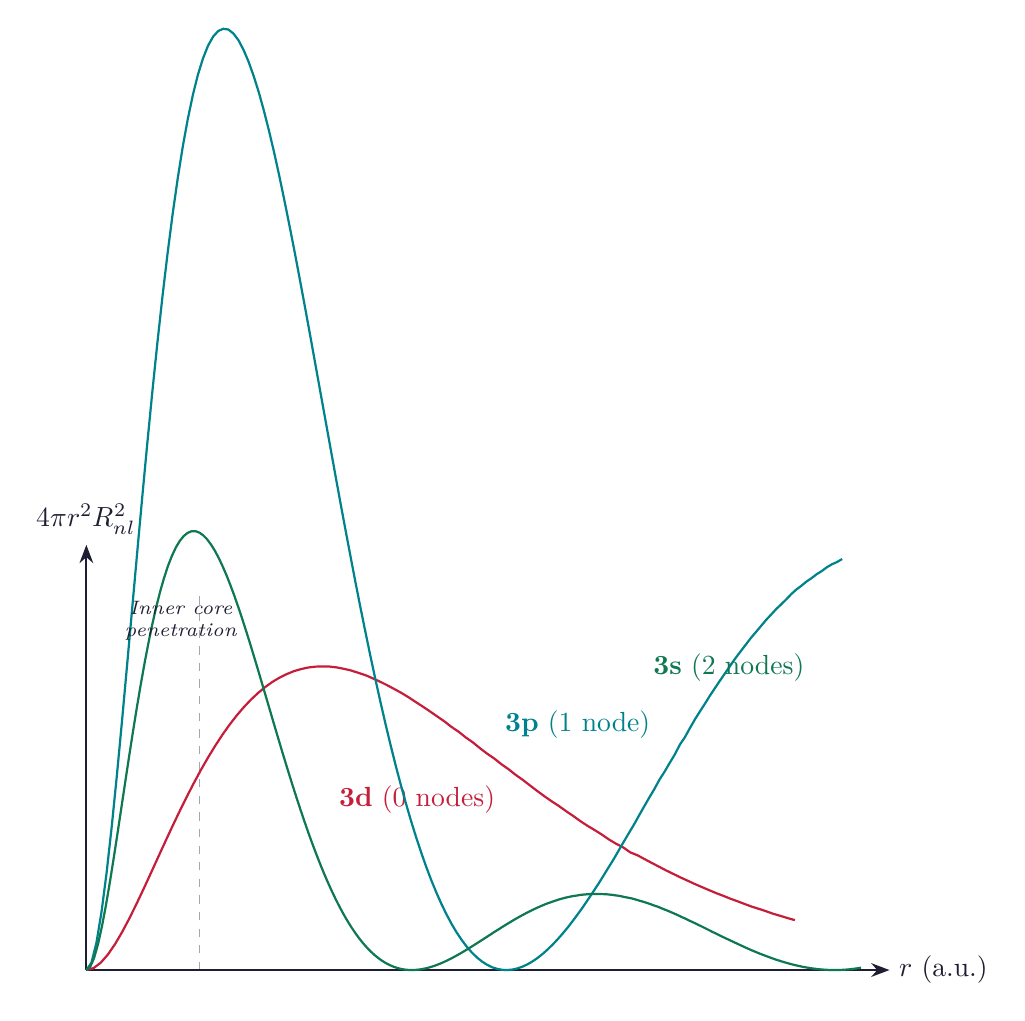
\begin{tikzpicture}[scale=1.2]
  % Draw axes
  \draw[arrow] (0,0) -- (8.5,0) node[right] {$r$ (a.u.)};
  \draw[arrow] (0,0) -- (0,4.5) node[above] {$4\pi r^2 R_{nl}^2$};
  
  % Plot 3d (1 peak, no nodes)
  \draw[thick, color=myred, domain=0:7.5, samples=100] 
    plot (\x, {3.8 * (\x)^2 * exp(-0.8*\x)});
  \node[color=myred] at (3.5, 1.8) {\textbf{3d} (0 nodes)};
  
  % Plot 3p (2 peaks, 1 node)
  \draw[thick, color=myteal, domain=0:8.0, samples=150] 
    plot (\x, {1.8 * (\x)^2 * (4 - 0.9*\x)^2 * exp(-0.7*\x)});
  \node[color=myteal] at (5.2, 2.6) {\textbf{3p} (1 node)};
  
  % Plot 3s (3 peaks, 2 nodes)
  \draw[thick, color=mygreen, domain=0:8.2, samples=200] 
    plot (\x, {0.6 * (\x)^2 * (6 - 2.5*\x + 0.22*(\x)^2)^2 * exp(-0.6*\x)});
  \node[color=mygreen] at (6.8, 3.2) {\textbf{3s} (2 nodes)};
  
  % Highlight penetration area close to nucleus
  \draw[dashed, color=mydark, opacity=0.4] (1.2, 0) -- (1.2, 4.0);
  \node[align=center, font=\scriptsize\itshape, color=mydark] at (1.0, 3.7) {Inner core\\penetration};
\end{tikzpicture}
\par\vspace{4pt}
\small\color{mydark}
Comparison of radial probability density distribution for $3s$, $3p$, and $3d$ orbitals. Note that while the main (outermost) peak of the $3d$ orbital is closer to the nucleus than that of $3s$, the $3s$ orbital has two inner peaks that penetrate the inner electron core, making $3s$ more stable (lower in energy).
\end{center}
\end{tcolorbox}

\subsection{Variations of Orbital Energies in the Periodic Table}
In hydrogenic atoms, the energy of an orbital depends solely on the principal quantum number $n$:
\[ E_n = -\frac{13.6 \cdot Z^2}{n^2}\ \text{eV} \]
Hence, $3s, 3p$, and $3d$ are degenerate (have the same energy).

In multi-electron atoms, the electrostatic shielding splits this degeneracy. The energy of an orbital depends on both $n$ and the azimuthal quantum number $l$. The ordering of orbital energies follows the $(n+l)$ rule (Madelung's rule):
\begin{enumerate}
  \item Orbitals are filled in order of increasing $(n+l)$ values.
  \item If two orbitals have the same $(n+l)$ value, the one with the lower $n$ value is filled first.
\end{enumerate}

Thus, for any shell $n$, the energy order is split by penetration and shielding into:
\[ E_{ns} < E_{np} < E_{nd} < E_{nf} \]

As the nuclear charge ($Z$) increases across the periodic table, the energies of all orbitals decrease (they become more stable) because the electrostatic attraction of the nucleus increases. However, they do not decrease at the same rate:
\begin{itemize}[leftmargin=*, itemsep=2pt]
  \item Inner shell orbitals drop rapidly in energy as $Z$ increases.
  \item Outer $s$ and $p$ orbitals drop steadily.
  \item $d$ and $f$ orbitals show a sudden, steep drop in energy (known as \textbf{orbital collapse}) when they begin to fill (e.g., $3d$ becomes lower in energy than $4s$ in transition metal cations).
\end{itemize}

\subsection{Electronic Configurations and Hund's Exchange Energy}
The ground-state electronic configuration of an atom is governed by three fundamental principles:
\begin{enumerate}
  \item \textbf{Aufbau Principle:} Electrons occupy the lowest energy orbitals available.
  \item \textbf{Pauli Exclusion Principle:} No two electrons in an atom can have the same set of four quantum numbers (an orbital can hold a maximum of 2 electrons with opposite spins).
  \item \textbf{Hund's Rule of Maximum Multiplicity:} For degenerate orbitals (orbitals with the same energy), the lowest energy configuration is the one that maximises the total spin multiplicity ($2S+1$). Electrons occupy degenerate orbitals singly with parallel spins before pairing begins.
\end{enumerate}

\textbf{Anomalous Electronic Configurations:}
Chromium ($Cr$, $Z=24$) and Copper ($Cu$, $Z=29$) are classic exceptions to the Aufbau rule:
\begin{itemize}[leftmargin=*, itemsep=1pt]
  \item Expected $Cr$: $[\text{Ar}]3d^4 4s^2$ \quad$\to$\quad Actual $Cr$: $[\text{Ar}]3d^5 4s^1$
  \item Expected $Cu$: $[\text{Ar}]3d^9 4s^2$ \quad$\to$\quad Actual $Cu$: $[\text{Ar}]3d^{10} 4s^1$
\end{itemize}

This anomalous behavior is driven by two main factors that stabilize half-filled ($d^5$) and fully-filled ($d^{10}$) subshells:
\begin{enumerate}
  \item \textbf{Symmetrical Distribution of Charge:} Symmetrical charge distribution around the nucleus reduces electron-electron repulsions and stabilizes the system.
  \item \textbf{Exchange Energy ($E_{\text{ex}}$):} Electrons with parallel spins in degenerate orbitals can exchange their positions. Each exchange releases a small quantum of energy called exchange energy, which stabilizes the atom. The number of possible exchanges ($P$) for $n$ parallel-spin electrons is given by:
  \begin{tcolorbox}[formulabox, title={Exchange Count Equation}]
    \[ P = \frac{n(n-1)}{2} \]
  \end{tcolorbox}
\end{enumerate}

\begin{tcolorbox}[examplebox, title={Example 2.1: Exchange Energy Comparison in Chromium ($Cr$)}]
  Compare the number of possible exchanges and stability between the expected and actual electronic configurations of Chromium ($Z=24$).
  \par\vspace{4pt}
  \textbf{Solution:}
  Let $K$ be the stabilizing exchange energy per exchange pair.
  \par\vspace{4pt}
  \textbf{Configuration A: $[\text{Ar}]3d^4 4s^2$ (Expected)}
  \begin{itemize}[leftmargin=*, itemsep=2pt]
    \item $3d^4$ subshell has 4 parallel-spin electrons ($\uparrow, \uparrow, \uparrow, \uparrow, \text{blank}$).
      \[ P_{3d} = \frac{4(4-1)}{2} = \frac{12}{2} = 6 \text{ exchanges} \]
    \item $4s^2$ has paired electrons ($\uparrow\downarrow$) which have opposite spins, so they cannot exchange.
    \item Total exchanges = $6$. Stabilization energy = $6K$.
  \end{itemize}
  \par\vspace{4pt}
  \textbf{Configuration B: $[\text{Ar}]3d^5 4s^1$ (Actual)}
  \begin{itemize}[leftmargin=*, itemsep=2pt]
    \item $3d^5$ subshell has 5 parallel-spin electrons ($\uparrow, \uparrow, \uparrow, \uparrow, \uparrow$).
      \[ P_{3d} = \frac{5(5-1)}{2} = \frac{20}{2} = 10 \text{ exchanges} \]
    \item $4s^1$ has 1 electron ($\uparrow$) which has a parallel spin to the $3d$ electrons. However, it resides in a different principal shell ($n=4$ vs $n=3$) and cannot exchange with $3d$.
    \item Total exchanges = $10$. Stabilization energy = $10K$.
  \end{itemize}
  \par\vspace{4pt}
  \textbf{Conclusion:} The actual configuration ($3d^5 4s^1$) has $10 - 6 = 4$ more exchanges than the expected configuration ($3d^4 4s^2$). The extra exchange energy ($4K$) easily overcomes the minor energy penalty of promoting an electron from $4s$ to $3d$, locking in the half-filled state.
\end{tcolorbox}

\begin{tcolorbox}[exambox, title={Exam Points: Penetration and Configurations}]
  \begin{itemize}[leftmargin=*, itemsep=2pt, topsep=2pt]
    \item \textbf{Penetration Order:} Always state the order $s > p > d > f$ and explain it using radial node count ($n-l-1$).
    \item \textbf{Energy splitting:} Explain why the $3s$ orbital is more stable than $3d$ in sodium despite having the same principal quantum number.
    \item \textbf{Exchange Energy:} Be ready to show the exchange energy calculation for $Cr$ or $Cu$ using the formula $P = \frac{n(n-1)}{2}$ to explain the stability of half/fully-filled shells.
    \item \textbf{Aufbau exceptions:} Clearly outline the configurations for $Cr$ ($3d^5 4s^1$) and $Cu$ ($3d^{10} 4s^1$).
  \end{itemize}
\end{tcolorbox}

% =============================================================================
\section{Atomic and Ionic Sizes}
% =============================================================================

\begin{tcolorbox}[defbox, title={Definitions: Types of Radii}]
  \textbf{Covalent Radius:} One-half of the distance between the nuclei of two identical atoms joined by a single covalent bond in a molecule (e.g., $d_{\text{Cl-Cl}} = 1.98\text{ \AA} \implies r_{\text{cov}} = 0.99\text{ \AA}$).
  \par\vspace{4pt}
  \textbf{Metallic (Crystal) Radius:} One-half of the internuclear distance between two adjacent metal cations in a metallic crystal lattice.
  \par\vspace{4pt}
  \textbf{Van der Waals Radius:} One-half of the closest internuclear distance between two non-bonded adjacent atoms belonging to two neighboring molecules in the solid state.
  \par\vspace{4pt}
  \textbf{Ionic Radius:} The effective distance from the center of the nucleus of an ion up to which it exerts influence on its electron cloud.
\end{tcolorbox}

\subsection{Comparison of Radii Types}
Because the van der Waals force is weak and non-binding, the nuclei of non-bonded adjacent atoms in a solid lattice remain relatively far apart. In contrast, covalent bonds involve significant overlap of valence electron clouds, drawing the nuclei close together. Metallic bonds represent an intermediate state where valence electrons are shared as a delocalized "sea." Therefore, for any given element, the relative sizes of these radii follow the order:

\begin{tcolorbox}[formulabox, title={Radii Comparison Trend}]
  \[ r_{\text{van der Waals}} > r_{\text{metallic}} > r_{\text{covalent}} \]
\end{tcolorbox}

\subsection{Periodic Trends in Atomic Sizes}
Atomic size is determined by the balance between the principal quantum number $n$ (which dictates the shell distance) and the effective nuclear charge $Z_{\text{eff}}$ (which pulls the shell closer).

\textbf{1. Across a Period (Left to Right):}
As we move across a period, $n$ remains constant while the effective nuclear charge $Z_{\text{eff}}$ increases by $\sim 0.65$ per element. The stronger electrostatic attraction pulls the electrons closer to the nucleus, causing the atomic radius to \textbf{decrease} steadily.

\textbf{2. Down a Group (Top to Bottom):}
As we move down a group, the principal quantum number $n$ increases (new energy shells are added). Although the nuclear charge increases, the shielding effect of the inner shells keeps $Z_{\text{eff}}$ relatively constant. The addition of new shells overrides the slight increases in $Z_{\text{eff}}$, causing the atomic radius to \textbf{increase} significantly.

\begin{tcolorbox}[tikzbox, title={Atomic Radii Trends Across Period 2 and Period 3}]
\begin{center}
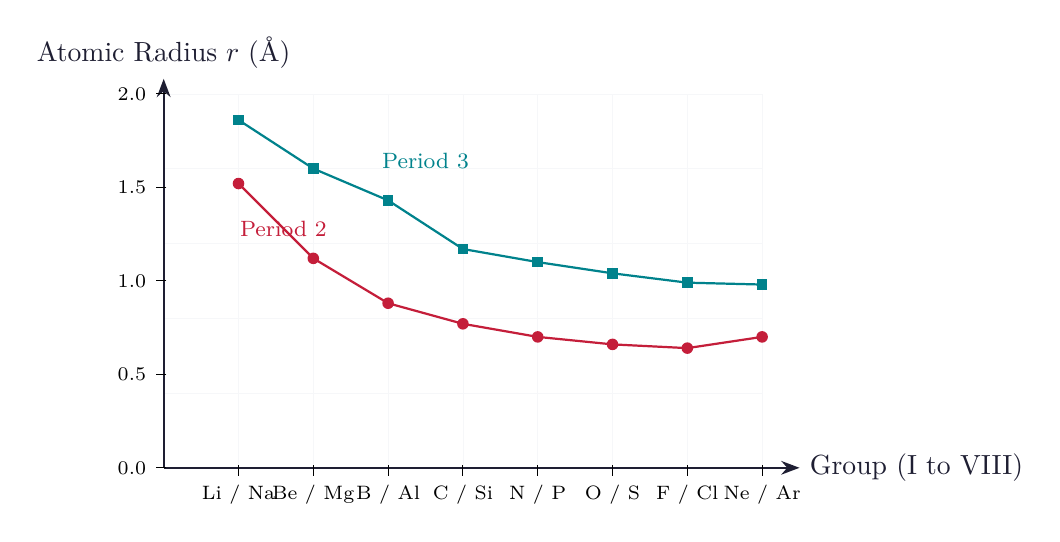
\begin{tikzpicture}[scale=0.95]
  % Draw Grid
  \draw[very thin, color=mygray, step=1.0] (0,0) grid (8,5);
  
  % Draw axes
  \draw[arrow] (0,0) -- (8.5,0) node[right] {Group (I to VIII)};
  \draw[arrow] (0,0) -- (0,5.2) node[above] {Atomic Radius $r$ (\text{\AA})};
  
  % Y-axis labels (0 to 2.0 A)
  \foreach \y/\label in {0/0.0, 1.25/0.5, 2.5/1.0, 3.75/1.5, 5.0/2.0} {
    \draw (1pt,\y) -- (-3pt,\y) node[left, font=\scriptsize] {\label};
  }
  
  % X-axis Group labels
  \foreach \x/\gp in {1/{Li / Na}, 2/{Be / Mg}, 3/{B / Al}, 4/{C / Si}, 5/{N / P}, 6/{O / S}, 7/{F / Cl}, 8/{Ne / Ar}} {
    \draw (\x,1pt) -- (\x,-3pt);
  }
  \node[below, font=\scriptsize] at (1, -0.1) {Li / Na};
  \node[below, font=\scriptsize] at (2, -0.1) {Be / Mg};
  \node[below, font=\scriptsize] at (3, -0.1) {B / Al};
  \node[below, font=\scriptsize] at (4, -0.1) {C / Si};
  \node[below, font=\scriptsize] at (5, -0.1) {N / P};
  \node[below, font=\scriptsize] at (6, -0.1) {O / S};
  \node[below, font=\scriptsize] at (7, -0.1) {F / Cl};
  \node[below, font=\scriptsize] at (8, -0.1) {Ne / Ar};

  % Period 2 Data: Li(1.52), Be(1.12), B(0.88), C(0.77), N(0.70), O(0.66), F(0.64), Ne(0.70)
  % Scaling: y_plot = y_val * 2.5
  \coordinate (P2_1) at (1, 3.8);  % Li
  \coordinate (P2_2) at (2, 2.8);  % Be
  \coordinate (P2_3) at (3, 2.2);  % B
  \coordinate (P2_4) at (4, 1.925); % C
  \coordinate (P2_5) at (5, 1.75); % N
  \coordinate (P2_6) at (6, 1.65); % O
  \coordinate (P2_7) at (7, 1.6);  % F
  \coordinate (P2_8) at (8, 1.75); % Ne (vdW)
  
  \draw[thick, color=myred] (P2_1) -- (P2_2) -- (P2_3) -- (P2_4) -- (P2_5) -- (P2_6) -- (P2_7) -- (P2_8);
  \foreach \i in {1,...,8} { \fill[color=myred] (P2_\i) circle (2.2pt); }
  \node[color=myred, font=\footnotesize] at (1.6, 3.2) {Period 2};

  % Period 3 Data: Na(1.86), Mg(1.60), Al(1.43), Si(1.17), P(1.10), S(1.04), Cl(0.99), Ar(0.98)
  % Scaling: y_plot = y_val * 2.5
  \coordinate (P3_1) at (1, 4.65); % Na
  \coordinate (P3_2) at (2, 4.0);  % Mg
  \coordinate (P3_3) at (3, 3.575);% Al
  \coordinate (P3_4) at (4, 2.925);% Si
  \coordinate (P3_5) at (5, 2.75); % P
  \coordinate (P3_6) at (6, 2.6);  % S
  \coordinate (P3_7) at (7, 2.475);% Cl
  \coordinate (P3_8) at (8, 2.45); % Ar (vdW)
  
  \draw[thick, color=myteal] (P3_1) -- (P3_2) -- (P3_3) -- (P3_4) -- (P3_5) -- (P3_6) -- (P3_7) -- (P3_8);
  \foreach \i in {1,...,8} { \fill[color=myteal] (P3_\i) +(-2pt,-2pt) rectangle +(2pt,2pt); }
  \node[color=myteal, font=\footnotesize] at (3.5, 4.1) {Period 3};

\end{tikzpicture}
\par\vspace{4pt}
\small\color{mydark}
Periodic atomic radii trends. Covalent radii decrease across Period 2 and 3. The noble gases (Ne, Ar) exhibit larger values than halogens because their radii are measured as non-bonding van der Waals radii, which do not involve orbital overlap.
\end{center}
\end{tcolorbox}

\subsection{Ionic Radii and Coordination Number Dependency}
Ionic radii depend heavily on the electric charge and configuration of the ion:
\begin{itemize}[leftmargin=*, itemsep=2pt]
  \item \textbf{Cations are always smaller than parent atoms:} Loss of valence electrons reduces electron-electron repulsion, allowing the remaining electrons to be pulled closer by the same nuclear charge (e.g., $r_{\text{Na}} = 1.86\text{ \AA}$ vs $r_{\text{Na}^+} = 1.02\text{ \AA}$).
  \item \textbf{Anions are always larger than parent atoms:} Gaining valence electrons increases electron-electron repulsions, expanding the electron cloud without any increase in nuclear charge (e.g., $r_{\text{Cl}} = 0.99\text{ \AA}$ vs $r_{\text{Cl}^-} = 1.81\text{ \AA}$).
\end{itemize}

\textbf{Coordination Number (CN) Dependency:}
An ion's radius is not a fixed constant. It varies with its coordination environment. As the coordination number (number of nearest neighbors) increases, the electrostatic repulsions between the surrounding ligands/ions squeeze the central ion less, or rather, the central ion must expand its coordination sphere to accommodate more ligands. Therefore, \textbf{ionic radius increases as the coordination number increases}. For example, the ionic radius of $\text{Li}^+$ increases from $0.59\text{ \AA}$ (for $\text{CN} = 4$) to $0.76\text{ \AA}$ (for $\text{CN} = 6$).

\subsection{Isoelectronic Series}
An isoelectronic series consists of atoms/ions that possess the same number of electrons but different nuclear charges ($Z$). 

For an isoelectronic series, the shielding constant $\sigma$ is essentially constant because the number and distribution of electrons are identical. Therefore, the effective nuclear charge experienced by the electrons is determined purely by the atomic number ($Z$). As $Z$ increases, the nuclear attraction pulls the same number of electrons closer. Thus, \textbf{in an isoelectronic series, size decreases as the atomic number ($Z$) increases}.

\begin{tcolorbox}[examplebox, title={Example 3.1: Isoelectronic Series Comparison}]
  Arrange the following species in order of decreasing size: $\text{O}^{2-}$, $\text{F}^-$, $\text{Na}^+$, $\text{Mg}^{2+}$, $\text{Al}^{3+}$.
  \par\vspace{4pt}
  \textbf{Solution:}
  All five species have exactly 10 electrons ($1s^2 2s^2 2p^6$) and are isoelectronic. We compile their nuclear charges ($Z$):
  \begin{center}
  \begin{tabularx}{0.8\linewidth}{|B{3cm}|Y|Y|Y|Y|Y|}
    \hline
    \textbf{Species} & $\text{O}^{2-}$ & $\text{F}^-$ & $\text{Na}^+$ & $\text{Mg}^{2+}$ & $\text{Al}^{3+}$ \\
    \hline
    \textbf{Nuclear Charge ($Z$)} & 8 & 9 & 11 & 12 & 13 \\
    \hline
    \textbf{Ionic Radius (\text{\AA})} & 1.40 & 1.33 & 1.02 & 0.72 & 0.54 \\
    \hline
  \end{tabularx}
  \end{center}
  As $Z$ increases from 8 to 13, the positive charge of the nucleus increases, pulling the 10 electrons tighter.
  \par\vspace{4pt}
  Therefore, the order of decreasing size is:
  \[ \text{O}^{2-} > \text{F}^- > \text{Na}^+ > \text{Mg}^{2+} > \text{Al}^{3+} \]
\end{tcolorbox}

\subsection{Lanthanide Contraction and Its Consequences}
The \textbf{Lanthanide Contraction} refers to the steady, progressive decrease in the atomic and ionic radii of the lanthanide elements (from Lanthanum ($Z=57$) to Lutetium ($Z=71$)) as the atomic number increases.

\textbf{Cause:}
As we move along the lanthanide series, electrons are added successively to the inner $4f$ subshell. The $4f$ orbitals are highly diffuse in space. As a result, the shielding of one $4f$ electron by another is extremely poor ($\sigma \approx 0.35$). However, with each element, the nuclear charge $Z$ increases by $+1$. Because the $4f$ electrons fail to screen the increasing positive charge, the effective nuclear charge felt by all outer electrons increases steadily. This pulls the outer shell closer, causing a steady contraction.

\textbf{Critical Consequences of Lanthanide Contraction:}
\begin{enumerate}
  \item \textbf{Size Similarity of $4d$ and $5d$ Elements:} In transition metal groups, we normally expect a significant increase in atomic size from the 2nd transition series ($4d$) to the 3rd transition series ($5d$) due to the addition of a new principal shell. However, the lanthanide contraction (which occurs between the $4d$ and $5d$ series) cancels out this expected increase.
    \par
    Consequently, elements of the 2nd and 3rd transition series in the same group have almost identical atomic and ionic radii.
    \begin{itemize}
      \item Group 4: $\text{Zr}$ ($4d$, $r \approx 1.60\text{ \AA}$) and $\text{Hf}$ ($5d$, $r \approx 1.59\text{ \AA}$).
      \item Group 5: $\text{Nb}$ ($4d$, $r \approx 1.46\text{ \AA}$) and $\text{Ta}$ ($5d$, $r \approx 1.46\text{ \AA}$).
    \end{itemize}
    This structural similarity makes their chemical separation extremely difficult.
  \item \textbf{Extreme Densities of Post-Lanthanide Metals:} Because the $5d$ transition elements have nearly identical sizes to their $4d$ counterparts but possess much higher atomic masses (due to 32 additional protons and neutrons), their densities are roughly double. For example, the density of Iridium ($22.56\ \text{g\,cm}^{-3}$) is twice that of Rhodium ($12.41\ \text{g\,cm}^{-3}$).
\end{enumerate}

\begin{tcolorbox}[exambox, title={Exam Points: Atomic and Ionic Sizes}]
  \begin{itemize}[leftmargin=*, itemsep=2pt, topsep=2pt]
    \item \textbf{Radii Comparison:} Explain why $r_{\text{vdW}} > r_{\text{met}} > r_{\text{cov}}$ using orbital overlap argument.
    \item \textbf{Isoelectronic Series:} Be prepared to write ionic size orders and explain them by referencing the nuclear charge ($Z$).
    \item \textbf{Lanthanide Contraction Cause:} State clearly that the cause is the "poor shielding of diffuse $4f$ orbitals."
    \item \textbf{Zr/Hf pair:} This is a MAKAUT favorite. Explain why Zr and Hf have identical properties by referencing the Lanthanide Contraction.
  \end{itemize}
\end{tcolorbox}

% =============================================================================
\section{Ionization Energy \& Electron Affinity}
% =============================================================================

\begin{tcolorbox}[defbox, title={Definitions: Ionization Energy and Electron Affinity}]
  \textbf{Ionization Energy (IE):} The minimum energy required to remove the most loosely bound electron from an isolated gaseous atom in its ground state:
  \[ \text{M(g)} + \text{IE} \to \text{M}^+\text{(g)} + e^- \]
  \par\vspace{4pt}
  \textbf{Electron Affinity (EA):} The amount of energy released when an electron is added to an isolated neutral gaseous atom to form a univalent anion:
  \[ \text{X(g)} + e^- \to \text{X}^-\text{(g)} + \text{EA} \]
  Its thermodynamic counterpart is \textbf{Electron Gain Enthalpy} ($\Delta_{\text{eg}}H \approx -\text{EA}$).
\end{tcolorbox}

\subsection{Successive Ionization Energies}
Removing successive electrons from an atom requires progressively larger amounts of energy. For any element, the successive ionization energies follow the order:
\[ IE_1 < IE_2 < IE_3 < IE_4 \dots \]

This trend is caused by:
\begin{enumerate}
  \item \textbf{Electrostatic Charge:} Removing an electron from a neutral atom ($IE_1$) only requires overcoming neutral forces. However, removing an electron from a positively charged cation ($IE_2$, $IE_3$) requires pulling a negative electron away from an increasingly positive net charge.
  \item \textbf{Size Contraction:} With each electron lost, electron-electron repulsion decreases, allowing the remaining orbital cloud to contract closer to the nucleus. This stronger binding increases the energy required for further ionization.
\end{enumerate}

A sudden, dramatic jump in successive ionization energies (e.g., $IE_2 \gg IE_1$ for Sodium) signifies the transition from removing valence-shell electrons to removing core-shell electrons from a highly stable noble-gas configuration.

\subsection{Factors Affecting Ionization Energy}
The ionization energy of an atom is determined by:
\begin{itemize}[leftmargin=*, itemsep=2pt]
  \item \textbf{Atomic Size:} As size increases, valence electrons are farther from the nucleus, experience less attraction, and are easier to remove ($\text{IE} \propto 1/r$).
  \item \textbf{Effective Nuclear Charge ($Z_{\text{eff}}$):} A higher $Z_{\text{eff}}$ pulls valence electrons tighter, increasing the energy needed to remove them ($\text{IE} \propto Z_{\text{eff}}$).
  \item \textbf{Penetration Effect:} Orbitals penetrate the inner electron core in the order $s > p > d > f$. An $s$ electron resides closer to the nucleus and experiences less shielding than a $p$ electron of the same shell, making it harder to ionize.
  \item \textbf{Electronic Configuration:} Half-filled ($d^5, p^3$) and fully-filled ($d^{10}, s^2$) subshells have extra stability due to exchange energy and symmetric charge distribution. Removing an electron from these stable configurations requires higher energy.
\end{itemize}

\subsection{Anomalies in Periodic IE Trends}
Across a period, ionization energy generally increases due to the steady increase in $Z_{\text{eff}}$. However, there are two distinct anomalies in every period:

\begin{tcolorbox}[examplebox, title={Anomaly 1: Beryllium ($Z=4$) vs. Boron ($Z=5$)}]
  Explain why the first ionization energy of Beryllium is higher than that of Boron ($IE_1(\text{Be}) = 899\ \text{kJ\,mol}^{-1}$ vs $IE_1(\text{B}) = 801\ \text{kJ\,mol}^{-1}$).
  \par\vspace{4pt}
  \textbf{Solution:}
  Let us inspect their ground-state configurations:
  \begin{itemize}[leftmargin=1cm, itemsep=2pt]
    \item $\text{Be}$: $1s^2 2s^2$ (fully-filled $2s$ subshell).
    \item $\text{B}$: $1s^2 2s^2 2p^1$ (partially-filled $2p$ subshell).
  \end{itemize}
  Two factors favor higher ionization energy for Beryllium:
  \begin{enumerate}
    \item \textbf{Penetration:} The electron to be removed from Beryllium resides in a $2s$ orbital, whereas the electron to be removed from Boron resides in a $2p$ orbital. Because $2s$ penetrates the inner core closer to the nucleus than $2p$, the $2s$ electron is bound more tightly.
    \item \textbf{Subshell Stability:} The $2s^2$ configuration of Beryllium is a fully-filled, closed-shell state which possesses extra electrostatic stability. Removing an electron disrupts this stable subshell.
  \end{enumerate}
  Therefore, Beryllium has a higher first ionization energy than Boron.
\end{tcolorbox}

\begin{tcolorbox}[examplebox, title={Anomaly 2: Nitrogen ($Z=7$) vs. Oxygen ($Z=8$)}]
  Explain why the first ionization energy of Nitrogen is higher than that of Oxygen ($IE_1(\text{N}) = 1402\ \text{kJ\,mol}^{-1}$ vs $IE_1(\text{O}) = 1314\ \text{kJ\,mol}^{-1}$).
  \par\vspace{4pt}
  \textbf{Solution:}
  Let us inspect their valence configurations:
  \begin{itemize}[leftmargin=1cm, itemsep=2pt]
    \item $\text{N}$: $2s^2 2p^3$ (half-filled $2p$ subshell: $2p_x^1 2p_y^1 2p_z^1$).
    \item $\text{O}$: $2s^2 2p^4$ (partially-filled $2p$ subshell: $2p_x^2 2p_y^1 2p_z^1$).
  \end{itemize}
  \begin{enumerate}
    \item \textbf{Exchange Energy:} Nitrogen has a stable, half-filled $2p^3$ configuration with 3 parallel-spin electrons. This configuration is stabilized by maximum exchange energy ($3$ exchange pairs) and symmetrical charge distribution.
    \item \textbf{Inter-electronic Repulsion:} In Oxygen's $2p^4$ configuration, one of the $2p$ orbitals ($2p_x$) contains a pair of electrons. These two electrons sharing the same orbital volume experience significant electrostatic repulsion. Removing one of these electrons relieves this repulsion and yields the highly stable half-filled $2p^3$ configuration.
  \end{enumerate}
  Consequently, it is easier to remove an electron from Oxygen than from Nitrogen, resulting in $IE_1(\text{N}) > IE_1(\text{O})$.
\end{tcolorbox}

\subsection{Electron Affinity and Successive Values}
Electron affinity (EA) measures the energy released when a gaseous atom gains an electron. If the process is exothermic, $\Delta_{\text{eg}}H$ is negative and EA is positive.

\textbf{Successive Electron Affinities:}
While the first electron affinity ($EA_1$) of most elements (like halogens, chalcogens) is positive (exothermic), the second electron affinity ($EA_2$) is \textbf{always highly negative (endothermic)}.
\par
For example, adding the first electron to Oxygen is exothermic:
\[ \text{O(g)} + e^- \to \text{O}^-\text{(g)} \quad \Delta_{\text{eg}}H_1 = -141\ \text{kJ\,mol}^{-1} \quad (EA_1 = +141\ \text{kJ\,mol}^{-1}) \]
However, adding the second electron to form oxide ($\text{O}^{2-}$) is highly endothermic:
\[ \text{O}^-\text{(g)} + e^- \to \text{O}^{2-}\text{(g)} \quad \Delta_{\text{eg}}H_2 = +780\ \text{kJ\,mol}^{-1} \quad (EA_2 = -780\ \text{kJ\,mol}^{-1}) \]
This occurs because the incoming electron experiences intense electrostatic repulsion from the existing negative charge of the $\text{O}^-$ anion. Overcoming this repulsion requires a significant input of energy. The formation of stable oxide lattices (like $\text{MgO}$ or $\text{Na}_2\text{O}$) in the solid state is driven by the very high lattice energy of the resulting ionic crystal, which easily compensates for this endothermic step.

\subsection{Anomalies in Electron Affinity Trends}
Within a group, electron affinity generally decreases down the column as atomic size increases, because the incoming electron is added farther from the nucleus. However, the elements of the \textbf{second period} (specifically F, O, N) exhibit anomalously low electron affinities compared to the elements of the \textbf{third period} (Cl, S, P):

\begin{tcolorbox}[examplebox, title={Anomaly: Fluorine vs. Chlorine Electron Affinity}]
  Explain why Chlorine has a higher electron affinity than Fluorine ($EA(\text{Cl}) = 349\ \text{kJ\,mol}^{-1}$ vs $EA(\text{F}) = 328\ \text{kJ\,mol}^{-1}$), even though Fluorine is smaller and more electronegative.
  \par\vspace{4pt}
  \textbf{Solution:}
  \begin{enumerate}
    \item \textbf{Valence Shell Volume:} Fluorine resides in the second period ($n=2$), and its valence electrons occupy a very compact $2p$ subshell. Chlorine resides in the third period ($n=3$), and its valence electrons occupy a much larger, more diffuse $3p$ subshell.
    \item \textbf{Inter-electronic Repulsion:} When an electron is added to the compact $2p$ subshell of Fluorine, the incoming electron experiences intense electrostatic repulsion from the seven electrons already packed in that small volume. This repulsion offsets some of the energy released by nuclear attraction.
    \item In Chlorine, the larger volume of the $3p$ subshell distributes the electron density over a wider area. The inter-electronic repulsion felt by the incoming electron is significantly lower.
  \end{enumerate}
  Therefore, more net energy is released when Chlorine gains an electron, resulting in $EA(\text{Cl}) > EA(\text{F})$.
\end{tcolorbox}

\subsection{Comparison Table: Ionization Energy vs. Electron Affinity}
\par\noindent
\begin{tabularx}{\linewidth}{|B{4.5cm}|Y|Y|}
\hline
\textbf{Property} & \textbf{Ionization Energy (IE)} & \textbf{Electron Affinity (EA)} \\
\hline
\textbf{Process} & Removal of an electron ($\text{M} \to \text{M}^+ + e^-$). & Addition of an electron ($\text{X} + e^- \to \text{X}^-$). \\
\hline
\textbf{Energy Change} & Always endothermic ($\Delta H > 0$, energy absorbed). & Usually exothermic for $EA_1$ ($\Delta H < 0$, energy released). Always endothermic for $EA_2$. \\
\hline
\textbf{Noble Gas Values} & Exceptionally high (stable closed-shell configurations). & Extremely low or negative (energy must be forced in to open a new shell). \\
\hline
\textbf{General Periodic Trend} & Increases across a period, decreases down a group. & Becomes more positive (exothermic) across a period, decreases down a group. \\
\hline
\textbf{Key Group 17 Anomaly} & $\text{IE}(\text{F}) > \text{IE}(\text{Cl})$ (normal size trend). & $\text{EA}(\text{Cl}) > \text{EA}(\text{F})$ (repulsion anomaly). \\
\hline
\end{tabularx}
\vspace{6pt}

\begin{tcolorbox}[exambox, title={Exam Points: IE and EA}]
  \begin{itemize}[leftmargin=*, itemsep=2pt, topsep=2pt]
    \item \textbf{Anomalous pairs:} Always explain Be/B and N/O in exams by writing down the subshell configurations.
    \item \textbf{F/Cl EA comparison:} This is the most common EA question. Focus on "charge density" and "inter-electronic repulsion in the compact $2p$ subshell of F."
    \item \textbf{Successive EA:} Explain why $EA_2$ is always negative (endothermic) by referencing the repulsion from the mono-negative anion.
    \item \textbf{IE Successive Trends:} Be ready to explain the massive jump in successive ionization energies (e.g. $IE_1$ vs $IE_2$ for alkali metals) as core-shell disruption.
  \end{itemize}
\end{tcolorbox}

% =============================================================================
\section{Electronegativity \& Polarizability}
% =============================================================================

\begin{tcolorbox}[defbox, title={Definitions: Electronegativity and Polarizability}]
  \textbf{Electronegativity ($\chi$):} The relative tendency of an atom in a molecule to attract the shared pair of electrons towards itself.
  \par\vspace{4pt}
  \textbf{Polarizing Power:} The ability of a cation to distort the electron cloud of an adjacent anion.
  \par\vspace{4pt}
  \textbf{Polarizability:} The ease with which the electron cloud of an anion can be distorted by a neighboring cation.
\end{tcolorbox}

\subsection{Electronegativity Scales}
Unlike ionization energy or electron affinity, electronegativity is not a direct thermodynamic property of an isolated atom. It represents a behavior within a bond, so it must be calculated using comparative scales:

\textbf{1. Pauling Scale (Bond Dissociation Energy Basis):}
Linus Pauling proposed that the excess bond energy of a polar bond $A-B$ over the average of pure homonuclear covalent bonds $A-A$ and $B-B$ is due to ionic-covalent resonance stabilization. The electronegativity difference is defined as:
\begin{tcolorbox}[formulabox, title={Pauling Electronegativity Difference}]
  \[ \chi_A - \chi_B = 0.102 \sqrt{\Delta} \]
  Where:
  \[ \Delta = E_{AB} - \sqrt{E_{AA} \cdot E_{BB}} \quad (\text{in kJ\,mol}^{-1}) \]
\end{tcolorbox}
Here, $\Delta$ represents the ionic resonance energy. Pauling arbitrarily assigned a value of $2.20$ to Hydrogen as an anchor to calibrate all other elements (Fluorine has the maximum value at $3.98$).

\textbf{2. Mulliken Scale (Atomic Energy Basis):}
Robert Mulliken proposed that an atom's ability to attract electrons in a bond is the average of its ionization energy (IE) and electron affinity (EA). If both values are measured in electron-volts ($\text{eV}$):
\begin{tcolorbox}[formulabox, title={Mulliken Electronegativity Equation}]
  \[ \chi_{\text{M}} = \frac{\text{IE} + \text{EA}}{2} \]
  To align Mulliken values with the Pauling scale:
  \[ \chi_{\text{P}} \approx \frac{\chi_{\text{M}}}{2.8} = \frac{\text{IE(eV)} + \text{EA(eV)}}{5.6} \]
\end{tcolorbox}
If IE and EA are in $\text{kJ\,mol}^{-1}$, the denominator is $540$.

\textbf{3. Allred-Rochow Scale (Electrostatic Force Basis):}
A. L. Allred and E. G. Rochow defined electronegativity as the electrostatic force of attraction exerted by the effective nuclear charge ($Z_{\text{eff}}$) of the atom on a valence electron at its bonding radius.
\begin{tcolorbox}[formulabox, title={Allred-Rochow Electronegativity Equation}]
  \[ \chi_{\text{AR}} = 0.359 \frac{Z_{\text{eff}}}{r^2} + 0.744 \]
  Where:
  \begin{itemize}[leftmargin=1.5cm, itemsep=1pt]
    \item[$Z_{\text{eff}}$] = Effective nuclear charge calculated using Slater's rules.
    \item[$r$] = Covalent radius of the atom (in \text{\AA}).
  \end{itemize}
\end{tcolorbox}

\begin{tcolorbox}[examplebox, title={Example 5.1: Calculation of Allred-Rochow Electronegativity for Carbon}]
  Calculate the Allred-Rochow electronegativity of Carbon given its covalent radius $r = 0.77\text{ \AA}$ and atomic number $Z = 6$.
  \par\vspace{4pt}
  \textbf{Solution:}
  \begin{enumerate}
    \item Calculate $Z_{\text{eff}}$ for a valence electron in Carbon using Slater's rules (from Example 1.1):
      \[ Z_{\text{eff}} = 3.25 \]
    \item Substitute $Z_{\text{eff}}$ and $r$ into the Allred-Rochow formula:
      \[ \chi_{\text{AR}} = 0.359 \left( \frac{3.25}{(0.77)^2} \right) + 0.744 \]
      \[ \chi_{\text{AR}} = 0.359 \left( \frac{3.25}{0.5929} \right) + 0.744 \approx 0.359 (5.48) + 0.744 \]
      \[ \chi_{\text{AR}} \approx 1.967 + 0.744 = 2.71 \]
  \end{enumerate}
  This calculated value ($2.71$) is very close to Carbon's experimental Pauling electronegativity ($2.55$).
\end{tcolorbox}

\subsection{Bond Character and the Hannay-Smith Equation}
The electronegativity difference between two bonded atoms determines the degree of polar covalent vs. ionic character in that bond. If $\Delta\chi = 0$, the bond is purely covalent. If $\Delta\chi > 1.7$, the bond is considered predominantly ionic.
\par
To calculate the percentage ionic character of a polar covalent bond, the \textbf{Hannay-Smith Equation} is used:

\begin{tcolorbox}[formulabox, title={Hannay-Smith Equation}]
  \[ \% \text{ Ionic Character} = 16 |\chi_A - \chi_B| + 3.5 |\chi_A - \chi_B|^2 \]
  Where $\chi_A$ and $\chi_B$ are the electronegativity values of the two bonded atoms.
\end{tcolorbox}

\begin{tcolorbox}[examplebox, title={Example 5.2: Calculating Ionic Character of Hydrogen Fluoride ($\text{HF}$)}]
  Calculate the percentage ionic character of the $\text{H-F}$ bond in hydrogen fluoride, given $\chi_{\text{F}} = 3.98$ and $\chi_{\text{H}} = 2.20$.
  \par\vspace{4pt}
  \textbf{Solution:}
  \begin{enumerate}
    \item Find the difference in electronegativity:
      \[ \Delta\chi = |\chi_{\text{F}} - \chi_{\text{H}}| = 3.98 - 2.20 = 1.78 \]
    \item Apply the Hannay-Smith equation:
      \[ \% \text{ Ionic Character} = 16 (1.78) + 3.5 (1.78)^2 \]
      \[ \% \text{ Ionic Character} = 28.48 + 3.5 (3.1684) \]
      \[ \% \text{ Ionic Character} = 28.48 + 11.09 = 39.57\% \]
  \end{enumerate}
  Thus, the bond in gaseous $\text{HF}$ is approximately $39.6\%$ ionic and $60.4\%$ covalent.
\end{tcolorbox}

\subsection{Polarizability and Fajans' Rules}
In an ideal ionic bond, electrons are completely transferred, producing spherical ions. However, in reality, when a small cation approaches a large anion, the positive charge of the cation attracts the outer electron cloud of the anion while repelling its nucleus. This distorts the anion's electron cloud, shifting electron density into the internuclear region, introducing covalent character into the ionic bond.

To predict the extent of this polarization (and thus the degree of covalent character), we use \textbf{Fajans' Rules}:

\begin{enumerate}
  \item \textbf{Small Cation Size:} A smaller cation has a higher charge density (charge-to-size ratio, $q/r$). It exerts a stronger electrostatic pull on the anion's electron cloud, increasing its polarizing power and covalent character (e.g., $\text{LiCl}$ is more covalent and soluble in organic solvents than $\text{KCl}$).
  \item \textbf{Large Anion Size:} In a large anion, the valence electrons are far from the nucleus and are shielded effectively by inner shells. The nucleus holds these electrons weakly, making the electron cloud soft and highly polarizable (e.g., $\text{LiI}$ is much more covalent than $\text{LiF}$).
  \item \textbf{High Ionic Charges:} High charges on either the cation or the anion increase the electrostatic attraction, driving stronger polarization and covalent character (e.g., $\text{AlCl}_3$ is covalent with a low melting point, whereas $\text{MgCl}_2$ and $\text{NaCl}$ are ionic).
  \item \textbf{Pseudo-Noble Gas Configuration of Cation ($ns^2 np^6 nd^{10}$):} Cations with a pseudo-noble gas configuration have greater polarizing power than those with a noble gas configuration ($ns^2 np^6$) of similar size and charge. This occurs because the $d$-electrons shield the nucleus poorly, allowing the cation to exert a stronger effective nuclear charge on the adjacent anion.
\end{enumerate}

\begin{tcolorbox}[examplebox, title={Example 5.3: Fajans' Rules Application}]
  Explain why Cuprous chloride ($\text{CuCl}$) is covalent and insoluble in water, whereas Sodium chloride ($\text{NaCl}$) is ionic and highly soluble, even though $\text{Cu}^+$ ($r = 0.96\text{ \AA}$) and $\text{Na}^+$ ($r = 0.95\text{ \AA}$) have nearly identical ionic sizes and identical charges.
  \par\vspace{4pt}
  \textbf{Solution:}
  Let us inspect the electronic configurations of the cations:
  \begin{itemize}[leftmargin=1cm, itemsep=2pt]
    \item $\text{Na}^+$: $1s^2 2s^2 2p^6$ (noble gas configuration, $8$-electron valence shell).
    \item $\text{Cu}^+$: $1s^2 2s^2 2p^6 3s^2 3p^6 3d^{10}$ (pseudo-noble gas configuration, $18$-electron valence shell).
  \end{itemize}
  The 10 electrons in the $3d$ subshell of $\text{Cu}^+$ are highly diffuse and shield the nuclear charge very poorly compared to the $s$ and $p$ electrons of $\text{Na}^+$. Consequently, $\text{Cu}^+$ has a much higher effective nuclear charge at its boundary. This allows it to polarize the electron cloud of the chloride ion ($\text{Cl}^-$) far more strongly than $\text{Na}^+$ can. This intense polarization introduces significant covalent character into $\text{CuCl}$, making it insoluble in polar water.
\end{tcolorbox}

\begin{tcolorbox}[exambox, title={Exam Points: Electronegativity and Fajans' Rules}]
  \begin{itemize}[leftmargin=*, itemsep=2pt, topsep=2pt]
    \item \textbf{Hannay-Smith Equation:} Memorize this equation ($16\Delta\chi + 3.5\Delta\chi^2$) for percentage ionic character calculations. It is a common numerical topic.
    \item \textbf{Allred-Rochow Scale:} Explain how it differs from Pauling and Mulliken scales by focusing on its physical basis (electrostatic force).
    \item \textbf{Fajans' Rules application:} Be prepared to explain melting point trends (e.g., why $\text{SnCl}_4$ is a liquid while $\text{SnCl}_2$ is a solid) or solubility trends using polarization.
    \item \textbf{Pseudo-noble gas configuration:} State clearly that $d$-electrons shield poorly, leading to higher polarizing power for cations like $\text{Cu}^+$, $\text{Ag}^+$, or $\text{Zn}^{2+}$.
  \end{itemize}
\end{tcolorbox}

% =============================================================================
\section{Oxidation States \& Coordination Numbers}
% =============================================================================

\begin{tcolorbox}[defbox, title={Definitions: Oxidation States, Coordination Numbers, and Geometries}]
  \textbf{Oxidation State (OS):} The formal charge assigned to an atom in a chemical species, assuming all bonding electron pairs are completely transferred to the more electronegative partner.
  \par\vspace{4pt}
  \textbf{Coordination Number (CN):} The number of donor atoms directly bonded (via coordinate or covalent bonds) to the central metal atom or ion in a coordination complex.
  \par\vspace{4pt}
  \textbf{Coordination Geometry:} The specific spatial arrangement of the ligand donor atoms around the central metal atom or ion.
\end{tcolorbox}

\subsection{Variable Oxidation States in Transition Metals}
One of the most defining characteristics of transition metals ($d$-block elements) is their ability to exhibit multiple, variable oxidation states. For instance, Manganese ($Mn$) shows all oxidation states from $+2$ to $+7$.

This behavior is caused by:
\begin{enumerate}
  \item \textbf{Orbital Energy Proximity:} The energy difference between the outer $ns$ orbital and the inner $(n-1)d$ orbital is extremely small.
  \item \textbf{Bond Participation:} Because of this energy proximity, transition metals can lose or share not only their valence $ns$ electrons but also their $(n-1)d$ electrons when forming chemical bonds.
\end{enumerate}

\textbf{Stability Trends in Transition Metal Oxidation States:}
\begin{itemize}[leftmargin=*, itemsep=2pt]
  \item \textbf{Valence Core Stability ($d^0$, $d^5$, $d^{10}$):} Oxidation states that leave the metal ion with a stable half-filled ($d^5$) or fully-filled ($d^{10}$) subshell, or a completely empty ($d^0$) noble-gas core, are particularly stable.
    \begin{itemize}
      \item $\text{Sc}^{3+}$ ($3d^0$, stable noble-gas $[\text{Ar}]$ configuration).
      \item $\text{Fe}^{3+}$ ($3d^5$, stable half-filled configuration) is more stable and harder to oxidize than $\text{Fe}^{2+}$ ($3d^6$).
      \item $\text{Zn}^{2+}$ ($3d^{10}$, stable fully-filled configuration).
    \end{itemize}
  \item \textbf{High vs. Low States:} The highest oxidation state shown by a transition metal in the first series ($3d$) corresponds to the loss of all $4s$ and $3d$ electrons (e.g., $+7$ for $\text{Mn}$, $+6$ for $\text{Cr}$). Beyond Manganese ($Z=25$), the $3d$ orbitals become steadily lower in energy and more core-like, so high oxidation states become unstable and transition metals favor lower oxidation states ($+2$, $+3$).
\end{itemize}

\subsection{The Inert Pair Effect in Heavier \texorpdfstring{$p$}{p}-Block Elements}
In the main group elements ($s$- and $p$-block), elements generally exhibit an oxidation state corresponding to their group number (e.g., $+3$ for Group 13, $+4$ for Group 14). However, for the heavier elements in these groups (specifically those in Period 6: Thallium, Lead, Bismuth), the most stable oxidation state is \textbf{two units lower} than the group oxidation state.

This phenomenon is called the \textbf{Inert Pair Effect}, which refers to the reluctance of the outermost $s$-orbital electron pair ($ns^2$) to participate in chemical bonding:

\begin{tcolorbox}[defbox, title={Stable Oxidation States due to Inert Pair Effect}]
  \begin{itemize}[leftmargin=*, itemsep=4pt]
    \item \textbf{Group 13 ($\text{Al}, \text{Ga}, \text{In}, \text{Tl}$):} Stable OS for $\text{Al}$ is $+3$, but for $\text{Tl}$, it is $+1$ ($\text{Tl}^+$ is stable, $\text{Tl}^{3+}$ is a powerful oxidizing agent).
    \item \textbf{Group 14 ($\text{Si}, \text{Ge}, \text{Sn}, \text{Pb}$):} Stable OS for $\text{Si}, \text{Sn}$ is $+4$, but for $\text{Pb}$, it is $+2$ ($\text{Pb}^{2+}$ is stable, $\text{Pb}^{4+}$ is a powerful oxidizing agent).
    \item \textbf{Group 15 ($\text{P}, \text{As}, \text{Sb}, \text{Bi}$):} Stable OS for $\text{P}$ is $+5$, but for $\text{Bi}$, it is $+3$ ($\text{Bi}^{3+}$ is stable, $\text{Bi}^{5+}$ is a powerful oxidizing agent).
  \end{itemize}
\end{tcolorbox}

\textbf{Underlying Cause:}
\begin{enumerate}
  \item \textbf{Poor Shielding:} The heavier post-transition elements (Period 6) contain filled $4f^{14}$ and $5d^{10}$ subshells. As established, $f$ and $d$ orbitals shield the nucleus very poorly.
  \item \textbf{Valence $s$-Orbital Contraction:} The high nuclear charge ($Z$) is not effectively screened, causing a very high effective nuclear charge $Z_{\text{eff}}$ to act on the outermost valence shell.
  \item Because $s$ orbitals ($l=0$) have the highest penetration power, they are drawn extremely close to the nucleus. This contraction stabilizes the $ns^2$ pair, making it inert and difficult to involve in chemical bonding. The energy released during chemical bonding (bond energy) is no longer enough to unpair and promote these $ns^2$ electrons.
\end{enumerate}

\subsection{Coordination Geometries and Hybridization}
The coordination number (CN) of a central metal ion dictates its local coordinate geometry. The valence bond theory (VBT) explains these geometries by matching them to specific orbital hybridizations:

\par\vspace{4pt}\noindent
\begin{tabularx}{\linewidth}{|B{2.2cm}|B{3.2cm}|Y|B{4.5cm}|}
\hline
\textbf{CN} & \textbf{Hybridization} & \textbf{Coordination Geometry} & \textbf{Example} \\
\hline
\textbf{2} & $sp$ & Linear & $[\text{Ag(NH}_3)_2]^+$ \\
\hline
\textbf{3} & $sp^2$ & Trigonal Planar & $[\text{HgI}_3]^-$ \\
\hline
\multirow{2}{*}{\textbf{4}} & $sp^3$ & Tetrahedral & $[\text{Ni(CO)}_4]$, $[\text{Zn(NH}_3)_4]^{2+}$ \\
\cline{2-4}
 & $dsp^2$ & Square Planar & $[\text{Ni(CN)}_4]^{2-}$, $[\text{PtCl}_4]^{2-}$ \\
\hline
\textbf{5} & $sp^3d$ & Trigonal Bipyramidal & $\text{Fe(CO)}_5$, $\text{PCl}_5$ \\
\hline
\textbf{6} & $sp^3d^2$ (or $d^2sp^3$) & Octahedral & $[\text{Fe(H}_2\text{O)}_6]^{3+}$, $[\text{Co(NH}_3)_6]^{3+}$ \\
\hline
\end{tabularx}
\vspace{6pt}

\begin{tcolorbox}[examplebox, title={Example 6.1: Inert Pair Effect Oxidation Reaction}]
  Explain why Lead dioxide ($\text{PbO}_2$, where $\text{Pb}$ is $+4$) reacts with concentrated hydrochloric acid to release chlorine gas, while Lead monoxide ($\text{PbO}$, where $\text{Pb}$ is $+2$) reacts normally without releasing chlorine.
  \par\vspace{4pt}
  \textbf{Solution:}
  \begin{enumerate}
    \item Due to the inert pair effect, the $+2$ oxidation state of Lead ($\text{Pb}^{2+}$) is highly stable, whereas the $+4$ state ($\text{Pb}^{4+}$) is unstable and behaves as a powerful oxidizing agent.
    \item In $\text{PbO}_2$, Lead is in the $+4$ oxidation state. It readily acts as an oxidizing agent, oxidizing chloride ions ($\text{Cl}^-$) from $\text{HCl}$ to elemental chlorine gas ($\text{Cl}_2$) while reducing itself to the stable $+2$ state:
      \[ \text{PbO}_2\text{(s)} + 4\text{HCl(aq)} \to \text{PbCl}_2\text{(s)} + \text{Cl}_2\text{(g)} + 2\text{H}_2\text{O(l)} \]
    \item In $\text{PbO}$, Lead is already in its stable $+2$ state. It has no tendency to undergo reduction, so it behaves as a simple basic oxide, reacting with $\text{HCl}$ in a standard acid-base neutralization:
      \[ \text{PbO\text{(s)}} + 2\text{HCl(aq)} \to \text{PbCl}_2\text{(s)} + \text{H}_2\text{O(l)} \]
  \end{enumerate}
\end{tcolorbox}

\begin{tcolorbox}[exambox, title={Exam Points: Oxidation States and CN}]
  \begin{itemize}[leftmargin=*, itemsep=2pt, topsep=2pt]
    \item \textbf{Transition metal oxidation states:} Explain why transition metals have variable states by referencing the small energy gap between $(n-1)d$ and $ns$ orbitals.
    \item \textbf{Inert Pair Effect definition:} Be ready to write the explanation focusing on "poor shielding of $d/f$ shells" and "outer $s$ orbital stabilization."
    \item \textbf{Oxidizing power:} Explain why $\text{Pb}^{4+}$ compounds are strong oxidizing agents whereas $\text{Sn}^{2+}$ compounds are strong reducing agents.
    \item \textbf{Coordination Geometries:} Memorize the hybridization and geometry mapping for coordination numbers 4 (distinguish between tetrahedral and square planar) and 6.
  \end{itemize}
\end{tcolorbox}

% =============================================================================
\section{Hard Soft Acids and Bases (HSAB) Principle}
% =============================================================================

\begin{tcolorbox}[defbox, title={Definitions: Pearson's HSAB Classification}]
  \textbf{Hard Acids:} Cations of small size, high charge, low polarizability, and high positive charge density. Their valence electrons are held tightly and are not easily distorted (e.g., $\text{H}^+$, $\text{Li}^+$, $\text{Na}^+$, $\text{Mg}^{2+}$, $\text{Al}^{3+}$, $\text{Fe}^{3+}$).
  \par\vspace{4pt}
  \textbf{Soft Acids:} Cations of large size, low or zero charge, high polarizability, and low positive charge density. Their valence electron cloud is easily distorted (e.g., $\text{Cu}^+$, $\text{Ag}^+$, $\text{Au}^+$, $\text{Hg}^{2+}$, $\text{Cd}^{2+}$, $\text{Pt}^{2+}$).
  \par\vspace{4pt}
  \textbf{Hard Bases:} Lewis bases containing highly electronegative donor atoms (O, N, F) of small size, which hold their electron pairs tightly, are highly resistant to oxidation, and have low polarizability (e.g., $\text{F}^-$, $\text{OH}^-$, $\text{H}_2\text{O}$, $\text{NH}_3$).
  \par\vspace{4pt}
  \textbf{Soft Bases:} Lewis bases containing less electronegative donor atoms (I, S, P) of large size, which have loosely bound electron pairs, are easily oxidized, and have high polarizability (e.g., $\text{I}^-$, $\text{H}^-$, $\text{S}^{2-}$, $\text{CN}^-$, $\text{PR}_3$).
\end{tcolorbox}

\subsection{Pearson's HSAB Principle}
Ralph G. Pearson proposed a simple qualitative rule in 1963 to predict the thermodynamic stability and reactivity of coordination complexes:

\begin{tcolorbox}[formulabox, title={Pearson's HSAB Principle}]
  \textbf{Statement:} Hard acids prefer to coordinate with hard bases, and soft acids prefer to coordinate with soft bases, to form stable chemical complexes.
\end{tcolorbox}

\subsection{Thermodynamic Basis of HSAB}
The preference of hard-hard and soft-soft combinations can be explained by the physical nature of the chemical bonds formed:

\begin{enumerate}
  \item \textbf{Hard-Hard Interactions (Electrostatic/Ionic):}
    Hard acids and hard bases are both small in size and possess high localized charges or electronegativity. The overlap between their orbitals is relatively poor due to the large energy gap. Instead, their interaction is dominated by \textbf{electrostatic (ionic) attraction}. The high positive charge density of the hard acid and high negative charge density of the hard base create a highly stable, strongly ionic lattice or complex, releasing substantial electrostatic potential energy.
  \item \textbf{Soft-Soft Interactions (Covalent):}
    Soft acids and soft bases are large, highly polarizable, and have similar electronegativities. The energy levels of their valence orbitals are very close, which allows for highly effective orbital overlap. Consequently, their interaction is dominated by \textbf{covalent bonding}. The mutual polarization of their soft electron clouds creates a stable, strongly covalent bond.
  \item \textbf{Hard-Soft Interactions (Unstable Mismatch):}
    A combination of a hard partner with a soft partner creates a mismatch. The bond is neither strongly ionic (due to the low charge density or low electronegativity of the soft partner) nor strongly covalent (due to the mismatch in orbital energies and polarizabilities). Thus, these complexes are thermodynamically less stable and react readily to swap partners.
\end{enumerate}

\subsection{Quantitative Hardness \texorpdfstring{($\eta$)}{(eta)} and Softness \texorpdfstring{($S$)}{(S)}}
In 1983, Pearson and Robert Parr quantified chemical hardness ($\eta$) using Density Functional Theory (DFT). They defined chemical hardness as the second derivative of the total energy of the system with respect to the number of electrons at constant nuclear potential. Operationally, it is calculated from the first ionization energy ($I$) and electron affinity ($A$):

\begin{tcolorbox}[formulabox, title={Chemical Hardness and Softness Equations}]
  \[ \eta = \frac{I - A}{2} \]
  Chemical softness ($S$) is defined simply as the reciprocal of hardness:
  \[ S = \frac{1}{\eta} = \frac{2}{I - A} \]
\end{tcolorbox}
A hard species has a large energy gap between its Homo (Highest Occupied Molecular Orbital) and Lumo (Lowest Occupied Molecular Orbital), representing high resistance to charge transfer. A soft species has a small Homo-Lumo gap, allowing for easy electron distortion and sharing.

\subsection{Applications of HSAB}

\textbf{1. Stability of Complexes:}
We can predict which complexes will form preferentially.
For example, the complex ion $[\text{AgI}_2]^-$ is highly stable, whereas $[\text{AgF}_2]^-$ is unstable and does not readily form in solution. This is because the silver ion ($\text{Ag}^+$) is a soft acid. It coordinates stably with the soft iodide ion ($\text{I}^-$) but forms an unstable mismatch with the hard fluoride ion ($\text{F}^-$).

\textbf{2. Predicting Direction of Reactions:}
Chemical reactions proceed to form more stable hard-hard and soft-soft pairs.
\par
Consider the exchange reaction:
\[ \text{LiI} + \text{CsF} \to \text{LiF} + \text{CsI} \]
Here, $\text{Li}^+$ is a hard acid, $\text{Cs}^+$ is a soft acid, $\text{F}^-$ is a hard base, and $\text{I}^-$ is a soft base. The reactants contain mismatched pairs ($\text{Li}^+-\text{I}^-$ is hard-soft; $\text{Cs}^+-\text{F}^-$ is soft-hard). The reaction proceeds spontaneously to the right to form the highly stable hard-hard pair ($\text{LiF}$) and soft-soft pair ($\text{CsI}$).

\textbf{3. Solubility of Halides:}
The solubility of metal halides in water can be explained by HSAB.
Silver iodide ($\text{AgI}$) is extremely insoluble in water, whereas Silver fluoride ($\text{AgF}$) is highly soluble. Water is a hard solvent (donor oxygen atom is hard).
In $\text{AgI}$, the soft-soft covalent interaction holds the lattice together very tightly, and the hard solvent water cannot solvate the soft ions effectively. In $\text{AgF}$, the hard-soft interaction is weak, and the hard fluoride ion is solvated extremely strongly by the hard water molecules, driving dissolution.

\textbf{4. Occurrence of Minerals in Nature:}
Geochemical elements are classified as lithophiles (rock-loving) or chalcophiles (ore-loving):
\begin{itemize}[leftmargin=*, itemsep=2pt]
  \item \textbf{Lithophilic metals:} Hard acids like $\text{Mg}^{2+}$, $\text{Al}^{3+}$, $\text{Ca}^{2+}$ occur in the Earth's crust as oxides, carbonates, or silicates. The oxygen donor atom in these anions is a hard base. Thus, they occur as stable hard-hard combinations.
  \item \textbf{Chalcophilic metals:} Soft acids like $\text{Cu}^+$, $\text{Pb}^{2+}$, $\text{Hg}^{2+}$, $\text{Zn}^{2+}$ occur predominantly as sulfide ores ($\text{Cu}_2\text{S}$, $\text{PbS}$, $\text{HgS}$, $\text{ZnS}$). The sulfur donor atom in sulfide ($\text{S}^{2-}$) is a soft base, resulting in stable soft-soft combinations.
\end{itemize}

\subsection{Summary of Classifications}
\par\noindent
\begin{tabularx}{\linewidth}{|B{3.2cm}|Y|Y|}
\hline
\textbf{Category} & \textbf{Hard Cases} & \textbf{Soft Cases} \\
\hline
\textbf{Acids (Cations)} & $\text{H}^+$, $\text{Li}^+$, $\text{Na}^+$, $\text{Mg}^{2+}$, $\text{Al}^{3+}$, $\text{Fe}^{3+}$, $\text{Cr}^{3+}$, $\text{Ti}^{4+}$ & $\text{Cu}^+$, $\text{Ag}^+$, $\text{Au}^+$, $\text{Hg}^{2+}$, $\text{Pt}^{2+}$, $\text{Pd}^{2+}$, $\text{Cd}^{2+}$ \\
\hline
\textbf{Bases (Anions)} & $\text{F}^-$, $\text{Cl}^-$, $\text{OH}^-$, $\text{H}_2\text{O}$, $\text{NH}_3$, $\text{CO}_3^{2-}$, $\text{SO}_4^{2-}$ & $\text{I}^-$, $\text{H}^-$, $\text{S}^{2-}$, $\text{CN}^-$, $\text{CO}$, $\text{PR}_3$, $\text{SCN}^-$ \\
\hline
\textbf{Borderline} & \multicolumn{2}{c|}{\textbf{Acids:} $\text{Fe}^{2+}$, $\text{Co}^{2+}$, $\text{Ni}^{2+}$, $\text{Zn}^{2+}$, $\text{Cu}^{2+}$, $\text{Pb}^{2+}$; \quad \textbf{Bases:} $\text{NO}_2^-$, $\text{SO}_3^{2-}$, $\text{py}$} \\
\hline
\end{tabularx}
\vspace{6pt}

\begin{tcolorbox}[examplebox, title={Example 7.1: Reactivity Prediction}]
  Predict the direction of the following reaction and explain it using the HSAB principle:
  \[ \text{HgF}_2 + \text{BeI}_2 \rightleftharpoons \text{HgI}_2 + \text{BeF}_2 \]
  \par\vspace{4pt}
  \textbf{Solution:}
  Let us identify the hard/soft nature of all participating ions:
  \begin{itemize}[leftmargin=1cm, itemsep=1pt]
    \item Cations: $\text{Hg}^{2+}$ is a large, polarizable cation (Soft Acid). $\text{Be}^{2+}$ is a very small cation with a high positive charge density (Hard Acid).
    \item Anions: $\text{F}^-$ is highly electronegative and small (Hard Base). $\text{I}^-$ is large and polarizable (Soft Base).
  \end{itemize}
  In the reactants:
  \begin{itemize}[leftmargin=1cm, itemsep=1pt]
    \item $\text{HgF}_2$ is a mismatched Soft Acid -- Hard Base pair.
    \item $\text{BeI}_2$ is a mismatched Hard Acid -- Soft Base pair.
  \end{itemize}
  In the products:
  \begin{itemize}[leftmargin=1cm, itemsep=1pt]
    \item $\text{HgI}_2$ is a highly stable Soft Acid -- Soft Base covalent combination.
    \item $\text{BeF}_2$ is a highly stable Hard Acid -- Hard Base ionic combination.
  \end{itemize}
  Therefore, the reaction spontaneous proceeds from left to right to swap the mismatched reactants into the stable products. The equilibrium lies heavily on the side of $\text{HgI}_2$ and $\text{BeF}_2$.
\end{tcolorbox}

\begin{tcolorbox}[exambox, title={Exam Points: HSAB Principle}]
  \begin{itemize}[leftmargin=*, itemsep=2pt, topsep=2pt]
    \item \textbf{Basic statement:} Always state Pearson's rule: "Hard prefers hard, soft prefers soft."
    \item \textbf{Bonding differences:} Explain that hard-hard is driven by electrostatic (ionic) forces, whereas soft-soft is driven by orbital overlap (covalent forces).
    \item \textbf{Geochemical occurrences:} This is a standard exam question. Explain why calcium occurs as calcium carbonate but copper occurs as copper sulfide using HSAB.
    \item \textbf{DFT definitions:} Know the equations for chemical hardness $\eta = (I-A)/2$ and softness $S = 1/\eta$.
  \end{itemize}
\end{tcolorbox}

% =============================================================================
\section{Molecular Geometries \& VSEPR Theory}
% =============================================================================

\begin{tcolorbox}[defbox, title={Definitions: VSEPR and Steric Number}]
  \textbf{VSEPR Theory:} A model used in chemistry to predict the geometry of individual molecules from the number of electron pairs surrounding their central atoms.
  \par\vspace{4pt}
  \textbf{Steric Number (SN):} The total number of bonding partners (single bonds, double bonds, etc., each counted as 1) and lone pairs surrounding the central atom:
  \[ \text{SN} = \text{Bonded Atoms} + \text{Lone Pairs} \]
\end{tcolorbox}

\subsection{Fundamental Postulates of VSEPR Theory}
Valence Shell Electron Pair Repulsion (VSEPR) theory was developed by Ronald Gillespie and Ronald Nyholm to predict molecular shapes based on the electrostatic repulsions of electron pairs:

\begin{enumerate}
  \item The spatial arrangement of bonds around the central atom is determined by the total number of valence shell electron pairs (bonding pairs and lone pairs).
  \item These electron pairs behave as charge clouds and orient themselves in space as far apart as possible to minimize electrostatic repulsion.
  \item \textbf{Repulsion Intensity Order:} Because lone pairs are attracted to only one nucleus, they are more spread out in space than bonding pairs, which are localized between two nuclei. Therefore, the repulsive forces between electron pairs follow the order:
    \begin{tcolorbox}[formulabox, title={VSEPR Repulsion Order}]
      \[ \text{lp--lp} > \text{lp--bp} > \text{bp--bp} \]
      \par\centering\small (Where: \; \text{lp} = \text{Lone Pair}, \; \text{bp} = \text{Bonding Pair})
    \end{tcolorbox}
  \item Double and triple bonds are treated as a single "super-active" bonding electron pair. The larger charge density of multiple bonds causes them to repel adjacent bonding/lone pairs more strongly than single bonds.
  \item Distortion of bond angles from ideal geometries (e.g., $109.5^\circ$ for tetrahedral, $120^\circ$ for trigonal planar) occurs when lone pairs or electronegativity differences introduce asymmetric repulsions.
\end{enumerate}

\subsection{Detailed Analysis of Molecular Geometries}

\textbf{1. Water ($\text{H}_2\text{O}$): $sp^3$ Hybridization, Bent (V-shaped) Shape}
\begin{itemize}[leftmargin=*, itemsep=1pt]
  \item Central atom: Oxygen ($1s^2 2s^2 2p^4$). It has 6 valence electrons.
  \item Bonds: 2 single bonds with Hydrogen, sharing 2 electrons.
  \item Electron pairs: $\text{SN} = 2\text{ (bp)} + 2\text{ (lp)} = 4$ electron pairs.
  \item Geometry: The 4 electron pairs point toward the corners of a tetrahedron. However, since two positions are occupied by lone pairs, the actual shape is \textbf{Bent (V-shaped)}.
  \item Angle: The ideal tetrahedral angle is $109.5^\circ$. The two lone pairs repel each other strongly ($\text{lp-lp}$ repulsion) and push the two $\text{O-H}$ bonding pairs closer together ($\text{lp-bp}$ repulsion), compressing the $\text{H-O-H}$ bond angle to $104.5^\circ$.
\end{itemize}

\textbf{2. Ammonia ($\text{NH}_3$): $sp^3$ Hybridization, Trigonal Pyramidal Shape}
\begin{itemize}[leftmargin=*, itemsep=1pt]
  \item Central atom: Nitrogen ($1s^2 2s^2 2p^3$). It has 5 valence electrons.
  \item Bonds: 3 single bonds with Hydrogen, sharing 3 electrons.
  \item Electron pairs: $\text{SN} = 3\text{ (bp)} + 1\text{ (lp)} = 4$ electron pairs.
  \item Geometry: The 4 electron pairs point toward the corners of a tetrahedron. Since one position is occupied by a lone pair, the molecular shape is \textbf{Trigonal Pyramidal}.
  \item Angle: The single lone pair repels the three $\text{N-H}$ bonding pairs ($\text{lp-bp}$ repulsion), compressing the $\text{H-N-H}$ bond angle from $109.5^\circ$ to $107.0^\circ$.
\end{itemize}

\textbf{3. Phosphorus Pentachloride ($\text{PCl}_5$): $sp^3d$ Hybridization, Trigonal Bipyramidal Shape}
\begin{itemize}[leftmargin=*, itemsep=1pt]
  \item Central atom: Phosphorus ($[\text{Ne}]3s^2 3p^3$). It has 5 valence electrons.
  \item Bonds: 5 single bonds with Chlorine, sharing 5 electrons.
  \item Electron pairs: $\text{SN} = 5\text{ (bp)} + 0\text{ (lp)} = 5$ electron pairs.
  \item Geometry: The molecular shape is an undistorted \textbf{Trigonal Bipyramidal}.
  \item Bond Length Inequality: There are two types of $\text{P-Cl}$ bonds:
    \begin{itemize}
      \item \textbf{Three Equatorial Bonds:} Lie in a flat plane at $120^\circ$ to each other (bond length $= 2.04\text{ \AA}$).
      \item \textbf{Two Axial Bonds:} Point straight up and down, perpendicular to the equatorial plane (bond length $= 2.19\text{ \AA}$).
    \end{itemize}
    The axial bonds are longer because they experience stronger electrostatic repulsions from the three equatorial bonds at $90^\circ$, whereas the equatorial bonds only experience repulsions from two axial bonds at $90^\circ$ and two equatorial bonds at $120^\circ$.
\end{itemize}

\begin{tcolorbox}[tikzbox, title={VSEPR Geometries (Part A): Tetrahedral-based and Octahedral-based}]
\begin{center}
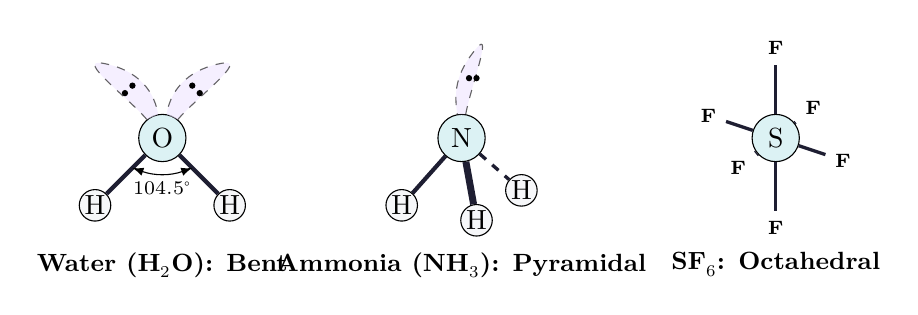
\begin{tikzpicture}[scale=0.95]
  % --- Water (Bent) ---
  \begin{scope}[xshift=-4.0cm, yshift=1.5cm]
    \node[draw, circle, fill=hdrteal, minimum size=0.6cm, inner sep=0pt] (O) at (0,0) {O};
    \node[draw, circle, fill=mygray, minimum size=0.4cm, inner sep=0pt] (H1) at (-0.9,-0.9) {H};
    \node[draw, circle, fill=mygray, minimum size=0.4cm, inner sep=0pt] (H2) at (0.9,-0.9) {H};
    
    \draw[line width=1.5pt, color=mydark] (O) -- (H1);
    \draw[line width=1.5pt, color=mydark] (O) -- (H2);
    
    % Draw lone pair lobes
    \draw[dashed, fill=hdrpurple, opacity=0.6] (O) to[out=50,in=10] (0.8,1.0) to[out=190,in=80] (O);
    \draw[dashed, fill=hdrpurple, opacity=0.6] (O) to[out=130,in=170] (-0.8,1.0) to[out=350,in=100] (O);
    \fill (0.4,0.7) circle (1.2pt); \fill (0.5,0.6) circle (1.2pt);
    \fill (-0.4,0.7) circle (1.2pt); \fill (-0.5,0.6) circle (1.2pt);
    
    % Angle label
    \draw[latex-latex, thin] (-0.4,-0.4) to[bend right=20] (0.4,-0.4);
    \node[below, font=\scriptsize] at (0,-0.45) {$104.5^\circ$};
    \node[below, font=\small\bfseries] at (0,-1.4) {Water ($\text{H}_2\text{O}$): Bent};
  \end{scope}

  % --- Ammonia (Trigonal Pyramidal) ---
  \begin{scope}[xshift=0.0cm, yshift=1.5cm]
    \node[draw, circle, fill=hdrteal, minimum size=0.6cm, inner sep=0pt] (N) at (0,0) {N};
    \node[draw, circle, fill=mygray, minimum size=0.4cm, inner sep=0pt] (H1) at (-0.8,-0.9) {H};
    \node[draw, circle, fill=mygray, minimum size=0.4cm, inner sep=0pt] (H2) at (0.2,-1.1) {H};
    \node[draw, circle, fill=mygray, minimum size=0.4cm, inner sep=0pt] (H3) at (0.8,-0.7) {H};
    
    \draw[line width=1.5pt, color=mydark] (N) -- (H1);
    \draw[line width=2.5pt, color=mydark] (N) -- (H2); % Wedged
    \draw[dashed, line width=1.2pt, color=mydark] (N) -- (H3); % Dashed
    
    % Lone pair lobe
    \draw[dashed, fill=hdrpurple, opacity=0.6] (N) to[out=80,in=50] (0.2,1.2) to[out=230,in=100] (N);
    \fill (0.1,0.8) circle (1.2pt); \fill (0.2,0.8) circle (1.2pt);
    
    \node[below, font=\small\bfseries] at (0,-1.4) {Ammonia ($\text{NH}_3$): Pyramidal};
  \end{scope}

  % --- Sulfur Hexafluoride (Octahedral) ---
  \begin{scope}[xshift=4.2cm, yshift=1.5cm]
    \node[draw, circle, fill=hdrteal, minimum size=0.6cm, inner sep=0pt] (S) at (0,0) {S};
    \node[font=\scriptsize\bfseries] (F1) at (0,1.2) {F};
    \node[font=\scriptsize\bfseries] (F2) at (0,-1.2) {F};
    \node[font=\scriptsize\bfseries] (F3) at (-0.9,0.3) {F};
    \node[font=\scriptsize\bfseries] (F4) at (0.9,-0.3) {F};
    \node[font=\scriptsize\bfseries] (F5) at (-0.5,-0.4) {F};
    \node[font=\scriptsize\bfseries] (F6) at (0.5,0.4) {F};
    
    \draw[line width=1.2pt, color=mydark] (S) -- (F1);
    \draw[line width=1.2pt, color=mydark] (S) -- (F2);
    \draw[line width=1.2pt, color=mydark] (S) -- (F3);
    \draw[line width=1.2pt, color=mydark] (S) -- (F4);
    \draw[line width=2.2pt, color=mydark] (S) -- (F5); % Wedged
    \draw[dashed, line width=1.2pt, color=mydark] (S) -- (F6); % Dashed
    
    \node[below, font=\small\bfseries] at (0,-1.4) {$\text{SF}_6$: Octahedral};
  \end{scope}
\end{tikzpicture}
\par\vspace{4pt}
\small\color{mydark}
3D orbital and bonding representations of tetrahedral-based shapes ($\text{H}_2\text{O}$ with 2 lone pairs; $\text{NH}_3$ with 1 lone pair) and octahedral geometry ($\text{SF}_6$ with 6 equivalent bonding directions).
\end{center}
\end{tcolorbox}

\textbf{4. Sulfur Tetrafluoride ($\text{SF}_4$): $sp^3d$ Hybridization, Seesaw Shape}
\begin{itemize}[leftmargin=*, itemsep=1pt]
  \item Central atom: Sulfur ($[\text{Ne}]3s^2 3p^4$). It has 6 valence electrons.
  \item Bonds: 4 single bonds with Fluorine, sharing 4 electrons.
  \item Electron pairs: $\text{SN} = 4\text{ (bp)} + 1\text{ (lp)} = 5$ electron pairs.
  \item Geometry: Based on a trigonal bipyramid. The single lone pair can occupy either an axial position or an equatorial position:
    \begin{itemize}
      \item \textbf{Axial lone pair:} Experiences three $90^\circ$ lone pair-bonding pair repulsions.
      \item \textbf{Equatorial lone pair:} Experiences only two $90^\circ$ lone pair-bonding pair repulsions.
    \end{itemize}
    To minimize electrostatic repulsions, the lone pair occupies the roomier \textbf{equatorial position}. The resulting shape is called a \textbf{Seesaw}.
  \item Distortion: The equatorial lone pair repels the axial and equatorial $\text{S-F}$ bonds, compressing the axial $\text{F-S-F}$ angle from $180^\circ$ to $173^\circ$, and the equatorial $\text{F-S-F}$ angle from $120^\circ$ to $101.5^\circ$.
\end{itemize}

\textbf{5. Chlorine Trifluoride ($\text{ClF}_3$): $sp^3d$ Hybridization, T-shaped Shape}
\begin{itemize}[leftmargin=*, itemsep=1pt]
  \item Central atom: Chlorine ($[\text{Ne}]3s^2 3p^5$). It has 7 valence electrons.
  \item Bonds: 3 single bonds with Fluorine, sharing 3 electrons.
  \item Electron pairs: $\text{SN} = 3\text{ (bp)} + 2\text{ (lp)} = 5$ electron pairs.
  \item Geometry: Based on a trigonal bipyramid. To minimize repulsions, both lone pairs occupy the \textbf{equatorial positions}. The three Fluorine atoms occupy the two axial and one equatorial positions, yielding a \textbf{T-shaped} molecule.
  \item Distortion: The two equatorial lone pairs exert strong repulsions, bending the axial $\text{F-Cl-F}$ bond axis slightly towards the equatorial Fluorine atom, compressing the axial-equatorial angles from $90^\circ$ to $87.5^\circ$.
\end{itemize}

\textbf{6. Xenon Difluoride ($\text{XeF}_2$): $sp^3d$ Hybridization, Linear Shape}
\begin{itemize}[leftmargin=*, itemsep=1pt]
  \item Central atom: Xenon ($5s^2 5p^6$). It has 8 valence electrons.
  \item Bonds: 2 single bonds with Fluorine, sharing 2 electrons.
  \item Electron pairs: $\text{SN} = 2\text{ (bp)} + 3\text{ (lp)} = 5$ electron pairs.
  \item Geometry: Based on a trigonal bipyramid. All three lone pairs occupy the three \textbf{equatorial positions} where they lie at $120^\circ$ to each other, cancelling their electrostatic repulsions. The two Fluorine atoms occupy the two axial positions. The molecular shape is perfectly \textbf{Linear} ($\text{F-Xe-F}$ bond angle $= 180^\circ$).
\end{itemize}

\textbf{7. Xenon Tetrafluoride ($\text{XeF}_4$): $sp^3d^2$ Hybridization, Square Planar Shape}
\begin{itemize}[leftmargin=*, itemsep=1pt]
  \item Central atom: Xenon ($5s^2 5p^6$). It has 8 valence electrons.
  \item Bonds: 4 single bonds with Fluorine, sharing 4 electrons.
  \item Electron pairs: $\text{SN} = 4\text{ (bp)} + 2\text{ (lp)} = 6$ electron pairs.
  \item Geometry: Based on an octahedron. The two lone pairs can be placed adjacent ($90^\circ$) or opposite ($180^\circ$) to each other.
    To minimize the strong lone pair-lone pair repulsion, the two lone pairs occupy the \textbf{axial positions} opposite each other ($180^\circ$). The four Fluorine atoms occupy the equatorial positions, yielding a symmetric \textbf{Square Planar} geometry (bond angles $= 90^\circ$).
\end{itemize}

\begin{tcolorbox}[tikzbox, title={VSEPR Geometries (Part B): Trigonal Bipyramidal-based shapes}]
\begin{center}
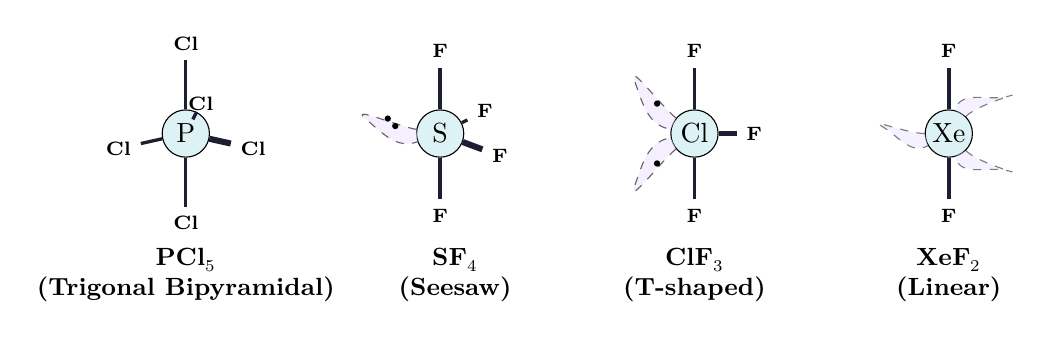
\begin{tikzpicture}[scale=0.95]
  % --- PCl5 (Trigonal Bipyramidal) ---
  \begin{scope}[xshift=-5.1cm]
    \node[draw, circle, fill=hdrteal, minimum size=0.6cm, inner sep=0pt] (P) at (0,0) {P};
    \node[font=\scriptsize\bfseries] (Cl1) at (0,1.2) {Cl};
    \node[font=\scriptsize\bfseries] (Cl2) at (0,-1.2) {Cl};
    \node[font=\scriptsize\bfseries] (Cl3) at (-0.9,-0.2) {Cl};
    \node[font=\scriptsize\bfseries] (Cl4) at (0.9,-0.2) {Cl};
    \node[font=\scriptsize\bfseries] (Cl5) at (0.2,0.4) {Cl};
    
    \draw[line width=1.2pt, color=mydark] (P) -- (Cl1);
    \draw[line width=1.2pt, color=mydark] (P) -- (Cl2);
    \draw[line width=1.2pt, color=mydark] (P) -- (Cl3);
    \draw[line width=2.2pt, color=mydark] (P) -- (Cl4); % Wedged
    \draw[dashed, line width=1.2pt, color=mydark] (P) -- (Cl5); % Dashed
    
    \node[below, font=\small\bfseries, align=center] at (0,-1.4) {$\text{PCl}_5$ \\ (Trigonal Bipyramidal)};
  \end{scope}

  % --- SF4 (Seesaw) ---
  \begin{scope}[xshift=-1.7cm]
    \node[draw, circle, fill=hdrteal, minimum size=0.6cm, inner sep=0pt] (S) at (0,0) {S};
    \node[font=\scriptsize\bfseries] (F1) at (0,1.1) {F};
    \node[font=\scriptsize\bfseries] (F2) at (0,-1.1) {F};
    \node[font=\scriptsize\bfseries] (F3) at (0.8,-0.3) {F};
    \node[font=\scriptsize\bfseries] (F4) at (0.6,0.3) {F};
    
    \draw[line width=1.2pt, color=mydark] (S) -- (F1);
    \draw[line width=1.2pt, color=mydark] (S) -- (F2);
    \draw[line width=2.2pt, color=mydark] (S) -- (F3); % Wedged
    \draw[dashed, line width=1.2pt, color=mydark] (S) -- (F4); % Dashed
    
    % Equatorial lone pair lobe
    \draw[dashed, fill=hdrpurple, opacity=0.6] (S) to[out=170,in=140] (-1.0,0.2) to[out=320,in=200] (S);
    \fill (-0.6,0.1) circle (1.2pt); \fill (-0.7,0.2) circle (1.2pt);
    
    \node[below, font=\small\bfseries, align=center] at (0.2,-1.4) {$\text{SF}_4$ \\ (Seesaw)};
  \end{scope}

  % --- ClF3 (T-shaped) ---
  \begin{scope}[xshift=1.7cm]
    \node[draw, circle, fill=hdrteal, minimum size=0.6cm, inner sep=0pt] (Cl) at (0,0) {Cl};
    \node[font=\scriptsize\bfseries] (F1) at (0,1.1) {F};
    \node[font=\scriptsize\bfseries] (F2) at (0,-1.1) {F};
    \node[font=\scriptsize\bfseries] (F3) at (0.8,0.0) {F};
    
    \draw[line width=1.2pt, color=mydark] (Cl) -- (F1);
    \draw[line width=1.2pt, color=mydark] (Cl) -- (F2);
    \draw[line width=1.5pt, color=mydark] (Cl) -- (F3);
    
    % Two equatorial lone pairs
    \draw[dashed, fill=hdrpurple, opacity=0.6] (Cl) to[out=140,in=110] (-0.8,0.7) to[out=290,in=170] (Cl);
    \draw[dashed, fill=hdrpurple, opacity=0.6] (Cl) to[out=220,in=250] (-0.8,-0.7) to[out=70,in=190] (Cl);
    \fill (-0.5,0.4) circle (1.2pt); \fill (-0.5,-0.4) circle (1.2pt);
    
    \node[below, font=\small\bfseries, align=center] at (0,-1.4) {$\text{ClF}_3$ \\ (T-shaped)};
  \end{scope}

  % --- XeF2 (Linear) ---
  \begin{scope}[xshift=5.1cm]
    \node[draw, circle, fill=hdrteal, minimum size=0.6cm, inner sep=0pt] (Xe) at (0,0) {Xe};
    \node[font=\scriptsize\bfseries] (F1) at (0,1.1) {F};
    \node[font=\scriptsize\bfseries] (F2) at (0,-1.1) {F};
    
    \draw[line width=1.5pt, color=mydark] (Xe) -- (F1);
    \draw[line width=1.5pt, color=mydark] (Xe) -- (F2);
    
    % Three equatorial lone pairs
    \draw[dashed, fill=hdrpurple, opacity=0.5] (Xe) to[out=180,in=150] (-0.9,0.1) to[out=330,in=210] (Xe);
    \draw[dashed, fill=hdrpurple, opacity=0.5] (Xe) to[out=45,in=15] (0.8,0.5) to[out=195,in=75] (Xe);
    \draw[dashed, fill=hdrpurple, opacity=0.5] (Xe) to[out=-45,in=-15] (0.8,-0.5) to[out=165,in=-75] (Xe);
    
    \node[below, font=\small\bfseries, align=center] at (0,-1.4) {$\text{XeF}_2$ \\ (Linear)};
  \end{scope}
\end{tikzpicture}
\par\vspace{4pt}
\small\color{mydark}
The evolution of shapes within the Steric Number 5 family ($\text{PCl}_5, \text{SF}_4, \text{ClF}_3, \text{XeF}_2$). Note that lone pairs always preferentially occupy the equatorial positions to minimize close $90^\circ$ repulsions.
\end{center}
\end{tcolorbox}

\subsection{Summary of SN and Molecular Shapes}
\par\vspace{4pt}\noindent
\begin{tabularx}{\linewidth}{|B{1.6cm}|B{2.2cm}|B{2.0cm}|B{2.8cm}|Y|}
\hline
\textbf{SN} & \textbf{Bond Pairs} & \textbf{Lone Pairs} & \textbf{Molecular Shape} & \textbf{Example} \\
\hline
\textbf{2} & 2 & 0 & Linear & $\text{CO}_2$, $\text{BeCl}_2$ \\
\hline
\multirow{2}{*}{\textbf{3}} & 3 & 0 & Trigonal Planar & $\text{BF}_3$, $\text{AlCl}_3$ \\
\cline{2-5}
 & 2 & 1 & Bent (V-shaped) & $\text{SO}_2$, $\text{O}_3$ \\
\hline
\multirow{3}{*}{\textbf{4}} & 4 & 0 & Tetrahedral & $\text{CH}_4$, $\text{SiCl}_4$ \\
\cline{2-5}
 & 3 & 1 & Trigonal Pyramidal & $\text{NH}_3$, $\text{PH}_3$ \\
\cline{2-5}
 & 2 & 2 & Bent (V-shaped) & $\text{H}_2\text{O}$, $\text{OF}_2$ \\
\hline
\multirow{4}{*}{\textbf{5}} & 5 & 0 & Trigonal Bipyramidal & $\text{PCl}_5$, $\text{SbF}_5$ \\
\cline{2-5}
 & 4 & 1 & Seesaw & $\text{SF}_4$, $\text{SeF}_4$ \\
\cline{2-5}
 & 3 & 2 & T-shaped & $\text{ClF}_3$, $\text{ICl}_3$ \\
\cline{2-5}
 & 2 & 3 & Linear & $\text{XeF}_2$, $\text{I}_3^-$ \\
\hline
\multirow{3}{*}{\textbf{6}} & 6 & 0 & Octahedral & $\text{SF}_6$, $\text{SeF}_6$ \\
\cline{2-5}
 & 5 & 1 & Square Pyramidal & $\text{BrF}_5$, $\text{IF}_5$ \\
\cline{2-5}
 & 4 & 2 & Square Planar & $\text{XeF}_4$, $\text{ICl}_4^-$ \\
\hline
\end{tabularx}
\vspace{6pt}

\begin{tcolorbox}[exambox, title={Exam Points: VSEPR and Shapes}]
  \begin{itemize}[leftmargin=*, itemsep=2pt, topsep=2pt]
    \item \textbf{Postulates:} State Gillespie-Nyholm rules clearly, emphasizing $\text{lp-lp} > \text{lp-bp} > \text{bp-bp}$ repulsion hierarchy.
    \item \textbf{Bond Angle Distortions:} Explain the angles of $\text{H}_2\text{O}$ ($104.5^\circ$) and $\text{NH}_3$ ($107^\circ$) by referencing lone pair repulsions.
    \item \textbf{Trigonal Bipyramid rule:} State clearly that lone pairs must occupy the equatorial positions first.
    \item \textbf{Bond length inequality in $\text{PCl}_5$:} Explain why axial bonds are longer than equatorial ones by counting $90^\circ$ repulsions.
    \item \textbf{Square Planar $\text{XeF}_4$:} Explain why the lone pairs occupy axial positions ($180^\circ$ apart) to minimize lp-lp repulsion.
  \end{itemize}
\end{tcolorbox}

\newpage
\begin{center}
  {\large\bfseries\color{myred} Quick Revision --- Module 5}\\[3pt]
  {\small\color{mydark} Periodic Properties $|$ BS-CH101}
\end{center}
\noindent{\color{myred}\rule{\linewidth}{1.2pt}}
\vspace{4pt}

\begin{tcolorbox}[formulabox, breakable, title={Key Formulas at a Glance},
  title after break={\textbf{Key Formulas at a Glance (contd.)}}]
\renewcommand{\arraystretch}{1.55}
\begin{tabularx}{\linewidth}{|B{4.5cm}|Y|}
\hline
\textbf{Formula} & \textbf{Meaning} \\
\hline
$Z_{\text{eff}} = Z - \sigma$ & Effective Nuclear Charge. \\
\hline
$\sigma = (n_{\text{same}} \times 0.35) + (n_{n-1} \times 0.85) + (n_{\text{inner}} \times 1.00)$ & Slater's rule for valence $(ns, np)$ electrons (except $1s$: $\sigma = 0.30$). \\
\hline
$\sigma = (n_{\text{same}} \times 0.35) + (n_{\text{left}} \times 1.00)$ & Slater's rule for $(nd)$ or $(nf)$ valence electrons. \\
\hline
$N_r = n - l - 1$ & Radial (spherical) nodes. \\
\hline
$N_a = l$ & Angular nodes (nodal planes). \\
\hline
$N_{\text{total}} = n - 1$ & Total nodes. \\
\hline
$P = \displaystyle\frac{n(n-1)}{2}$ & Hund's rule: possible exchange count for $n$ parallel-spin electrons. \\
\hline
$\chi_A - \chi_B = 0.102 \sqrt{\Delta}$ & Pauling electronegativity difference ($\Delta$ in $\text{kJ\,mol}^{-1}$). \\
\hline
$\Delta = E_{AB} - \sqrt{E_{AA} \cdot E_{BB}}$ & Pauling's ionic resonance stabilization energy. \\
\hline
$\chi_{\text{M}} = \displaystyle\frac{\text{IE} + \text{EA}}{2}$ & Mulliken electronegativity ($\text{IE}$, $\text{EA}$ in $\text{eV}$). \\
\hline
$\chi_{\text{P}} \approx \displaystyle\frac{\text{IE(eV)} + \text{EA(eV)}}{5.6}$ & Mulliken-to-Pauling electronegativity scale conversion. \\
\hline
$\chi_{\text{P}} \approx \displaystyle\frac{\text{IE} + \text{EA}}{540}$ & Mulliken-to-Pauling conversion ($\text{IE}$, $\text{EA}$ in $\text{kJ\,mol}^{-1}$). \\
\hline
$\chi_{\text{AR}} = 0.359 \displaystyle\frac{Z_{\text{eff}}}{r^2} + 0.744$ & Allred-Rochow electronegativity ($r$ in \text{\AA}). \\
\hline
$\% \text{ Ionic Character} = 16 |\chi_A - \chi_B| + 3.5 |\chi_A - \chi_B|^2$ & Hannay-Smith equation. \\
\hline
$\% \text{ Ionic Character} = 100 \left(1 - e^{-0.25(\chi_A - \chi_B)^2}\right)$ & Pauling's ionic character formula. \\
\hline
$\eta = \displaystyle\frac{I - A}{2}$ & DFT Chemical Hardness ($I = \text{IE}$, $A = \text{EA}$). \\
\hline
$S = \displaystyle\frac{1}{\eta} = \displaystyle\frac{2}{I - A}$ & DFT Chemical Softness. \\
\hline
$\text{SN} = \text{Bonded Atoms} + \text{Lone Pairs}$ & Steric Number for VSEPR/hybridization. \\
\hline
$\phi = \displaystyle\frac{q}{r}$ & Ionic potential (charge density) for Fajans' polarization. \\
\hline
\end{tabularx}
\end{tcolorbox}

\begin{tcolorbox}[defbox, title={One-Line Definitions}]
\begin{itemize}[leftmargin=*, itemsep=2.pt, topsep=2pt]
  \item \textbf{Shielding effect:} The screening of outer electrons from nuclear attraction by inner electrons.
  \item \textbf{Effective nuclear charge ($Z_{\text{eff}}$):} The net positive charge experienced by an electron in a multi-electron atom.
  \item \textbf{Penetration power:} The relative probability density of finding an orbital's electron close to the nucleus.
  \item \textbf{Radial node:} A spherical surface around the nucleus where the electron probability density is zero.
  \item \textbf{Aufbau principle:} The rule stating that electrons fill subshells in order of increasing $(n+l)$ energy.
  \item \textbf{Pauli exclusion principle:} A rule stating that no two electrons in an atom can have the same four quantum numbers.
  \item \textbf{Hund's rule:} Degenerate orbitals are filled singly with parallel spins before electron pairing begins.
  \item \textbf{Exchange energy:} The electrostatic stabilization energy released when parallel-spin electrons swap degenerate positions.
  \item \textbf{Covalent radius:} One-half of the distance between the nuclei of two identical single-bonded atoms.
  \item \textbf{Metallic radius:} One-half of the distance between adjacent metal cations in a crystal lattice.
  \item \textbf{Van der Waals radius:} One-half of the closest distance between non-bonded adjacent atoms in a solid lattice.
  \item \textbf{Ionic radius:} The effective distance from an ion's nucleus where it exerts electrostatic control over its electron cloud.
  \item \textbf{Lanthanide contraction:} The steady contraction in atomic and ionic radii along the lanthanide series ($La \to Lu$).
  \item \textbf{Isoelectronic species:} Atoms or ions sharing the same number and distribution of electrons.
  \item \textbf{Ionization energy:} The minimum energy required to remove the most loosely bound electron from a gaseous atom.
  \item \textbf{Successive ionization energies:} Energies required to remove further electrons sequentially ($IE_1 < IE_2 < IE_3 \dots$).
  \item \textbf{Electron affinity:} The energy released when an electron is added to a neutral gaseous atom.
  \item \textbf{Electron gain enthalpy ($\Delta_{\text{eg}}H$):} The enthalpy change accompanying the addition of an electron to an atom.
  \item \textbf{Electronegativity:} The tendency of an atom in a molecule to attract the shared bonding electron pair.
  \item \textbf{Polarizing power:} The ability of a cation to distort the electron cloud of an adjacent anion.
  \item \textbf{Polarizability:} The susceptibility of an anion's electron cloud to distortion by a cation.
  \item \textbf{Fajans' rules:} A set of empirical rules predicting the degree of covalent character in an ionic bond.
  \item \textbf{Pseudo-noble gas configuration:} Cation valence configurations with 18 electrons ($ns^2 np^6 nd^{10}$).
  \item \textbf{Oxidation state:} The formal charge an atom would carry if all bonds were purely ionic.
  \item \textbf{Coordination number:} The number of donor atoms directly bonded to a central metal ion.
  \item \textbf{Coordination geometry:} The spatial arrangement of coordinating ligands around the central metal ion.
  \item \textbf{Inert pair effect:} The reluctance of the outermost valence $ns^2$ pair to participate in chemical bonding in heavier post-transition metals.
  \item \textbf{Hard acid/base:} Cations/anions of small size and low polarizability.
  \item \textbf{Soft acid/base:} Cations/anions of large size and high polarizability.
  \item \textbf{Steric number:} The sum of bonded atoms and lone pairs around a central atom in VSEPR theory.
\end{itemize}
\end{tcolorbox}

\begin{tcolorbox}[exambox, title={Frequently Asked / Viva Questions}]
  \Q{Q1. Why is the first ionization energy of Nitrogen greater than that of Oxygen?}
  Nitrogen has a stable, half-filled $2p^3$ subshell ($2p_x^1 2p_y^1 2p_z^1$) which possesses high exchange energy. Oxygen has $2p^4$, containing a paired electron in the $2p_x$ orbital. The inter-electronic repulsion between these paired electrons makes it easier to remove an electron from Oxygen, resulting in $IE_1(\text{N}) > IE_1(\text{O})$.
  \par\vspace{6pt}
  \Q{Q2. Why does Chlorine have a higher electron affinity than Fluorine?}
  Fluorine is extremely small, and its valence electrons occupy a highly compact $2p$ subshell. Adding an electron to this small volume causes intense inter-electronic repulsion, which offsets some of the energy released. Chlorine is larger and its diffuse $3p$ subshell accommodates the incoming electron with much less repulsion, releasing more net energy.
  \par\vspace{6pt}
  \Q{Q3. What is the cause of the Lanthanide Contraction?}
  The addition of electrons to the inner $4f$ subshell. The $4f$ orbitals are diffuse and shield the increasing nuclear charge ($+1$ per element) very poorly. Consequently, the effective nuclear charge felt by outer electrons increases steadily, contracting the shell.
  \par\vspace{6pt}
  \Q{Q4. Explain why Zirconium ($\text{Zr}$) and Hafnium ($\text{Hf}$) have almost identical atomic radii.}
  Hafnium ($5d$, $Z=72$) follows the lanthanides ($La \to Lu$). The intervening 14 lanthanide elements undergo a steady atomic shrinkage (lanthanide contraction). This shrinkage cancels out the normal size increase expected from adding a new principal shell, making $r_{\text{Zr}} \approx r_{\text{Hf}}$.
  \par\vspace{6pt}
  \Q{Q5. Why is the first ionization energy of Beryllium greater than that of Boron?}
  Beryllium ($1s^2 2s^2$) has a fully-filled $2s$ subshell. The valence electron is removed from a $2s$ orbital, which is more penetrating and bound tighter than the $2p$ valence electron in Boron ($1s^2 2s^2 2p^1$).
  \par\vspace{6pt}
  \Q{Q6. State Fajans' rules for covalent character in ionic compounds.}
  Covalent character increases with: (i) small cation size, (ii) large anion size, (iii) high charges on the ions, and (iv) pseudo-noble gas configurations ($ns^2 np^6 nd^{10}$) of the cation.
  \par\vspace{6pt}
  \Q{Q7. Explain why $\text{CuCl}$ is insoluble in water whereas $\text{NaCl}$ is soluble.}
  $\text{Cu}^+$ has a pseudo-noble gas configuration ($3d^{10}$). The $d$-electrons shield the nucleus poorly, giving $\text{Cu}^+$ a higher polarizing power than $\text{Na}^+$ (noble gas configuration). This strong polarization introduces covalent character in $\text{CuCl}$, making it insoluble in water.
  \par\vspace{6pt}
  \Q{Q8. What is the inert pair effect?}
  The reluctance of the outermost $ns^2$ valence pair to participate in chemical bonding in heavier post-transition elements of Groups 13-15 (Tl, Pb, Bi) due to poor shielding by $d/f$ subshells and valence shell contraction.
  \par\vspace{6pt}
  \Q{Q9. Why is $\text{PbO}_2$ a strong oxidizing agent while $\text{PbO}$ is stable?}
  Due to the inert pair effect, the stable oxidation state for Lead is $+2$. Lead in the $+4$ state ($\text{PbO}_2$) is unstable and acts as a powerful oxidizing agent to reduce itself to the stable $+2$ state ($\text{Pb}^{2+}$).
  \par\vspace{6pt}
  \Q{Q10. State the Pearson HSAB principle.}
  Hard acids prefer to coordinate with hard bases (forming stable ionic bonds), and soft acids prefer to coordinate with soft bases (forming stable covalent bonds).
  \par\vspace{6pt}
  \Q{Q11. Explain why calcium occurs as $\text{CaCO}_3$ in nature but copper occurs as $\text{Cu}_2\text{S}$.}
  $\text{Ca}^{2+}$ is a hard acid and coordinates stably with the hard base carbonate ($\text{CO}_3^{2-}$). $\text{Cu}^+$ is a soft acid and coordinates stably with the soft base sulfide ($\text{S}^{2-}$).
  \par\vspace{6pt}
  \Q{Q12. Why is $\text{AgI}$ insoluble in water but $\text{AgF}$ is soluble?}
  $\text{Ag}^+$ and $\text{I}^-$ are both soft. The soft-soft covalent lattice in $\text{AgI}$ is highly stable and cannot be broken by the hard solvent water. In $\text{AgF}$, the mismatched hard-soft interaction is weak, and the hard $\text{F}^-$ is strongly hydrated, driving dissolution.
  \par\vspace{6pt}
  \Q{Q13. State the postulates of VSEPR theory.}
  Valence electron pairs (bonding and lone pairs) around a central atom repel each other and orient in space to maximize distance and minimize repulsion.
  \par\vspace{6pt}
  \Q{Q14. What is the order of repulsive forces between electron pairs in VSEPR?}
  $\text{Lone Pair -- Lone Pair (lp-lp)} > \text{Lone Pair -- Bonding Pair (lp-bp)} > \text{Bonding Pair -- Bonding Pair (bp-bp)}$.
  \par\vspace{6pt}
  \Q{Q15. Why is the bond angle of $\text{H}_2\text{O}$ ($104.5^\circ$) smaller than that of $\text{NH}_3$ ($107^\circ$)?}
  Water has two lone pairs on Oxygen which repel each other and compress the bonding pairs strongly. Ammonia has only one lone pair on Nitrogen, which exerts less compressive repulsion.
  \par\vspace{6pt}
  \Q{Q16. Why are the axial $\text{P-Cl}$ bonds in $\text{PCl}_5$ longer than the equatorial ones?}
  The two axial chlorine atoms experience stronger electrostatic repulsions from the three equatorial chlorine atoms at $90^\circ$, forcing the axial bonds to lengthen to minimize repulsions.
  \par\vspace{6pt}
  \Q{Q17. What is the shape of $\text{SF}_4$?}
  Seesaw. The lone pair occupies an equatorial position to minimize $90^\circ$ repulsions (it experiences only two $90^\circ$ repulsions, compared to three if it were axial).
  \par\vspace{6pt}
  \Q{Q18. What are isoelectronic species? Give an example.}
  Atoms or ions containing the same number of electrons. Example: $\text{N}^{3-}, \text{O}^{2-}, \text{F}^-, \text{Na}^+, \text{Mg}^{2+}$, all of which have 10 electrons.
  \par\vspace{6pt}
  \Q{Q19. Why does ionic radius increase with coordination number?}
  A higher coordination number requires the central ion to expand its coordination sphere to accommodate more ligands, reducing steric repulsions and effectively increasing its radius.
  \par\vspace{6pt}
  \Q{Q20. Write the Slater's rules groupings.}
  $(1s) \; (2s, 2p) \; (3s, 3p) \; (3d) \; (4s, 4p) \; (4d) \; (4f) \; (5s, 5p) \; (5d) \dots$
  \par\vspace{6pt}
  \Q{Q21. Why are $s$-electrons more penetrating than $p$-electrons?}
  The angular momentum barrier is zero for $s$-orbitals ($l=0$). This allows the radial wavefunction of $s$-orbitals to have significant density peaks very close to the nucleus.
  \par\vspace{6pt}
  \Q{Q22. Define chemical hardness and write its operational formula.}
  Resistance of a chemical species to charge transfer and polarization. Formula: $\eta = (I-A)/2$.
  \par\vspace{6pt}
  \Q{Q23. Why do noble gases have positive electron gain enthalpies?}
  Noble gases have stable, closed-shell configurations ($ns^2 np^6$). Adding an electron requires forcing it into a higher principal energy shell ($n+1$), which is highly endothermic.
  \par\vspace{6pt}
  \Q{Q24. Why is $\text{ClF}_3$ T-shaped and not trigonal planar?}
  The central Chlorine has 5 electron pairs ($\text{SN} = 5$). To minimize repulsions, the two lone pairs occupy equatorial positions, leaving the three Fluorine atoms to form a T-shape.
  \par\vspace{6pt}
  \Q{Q25. Why is $\text{XeF}_4$ square planar?}
  Xenon has 6 electron pairs ($\text{SN} = 6$). The two lone pairs occupy axial positions directly opposite each other ($180^\circ$ apart) to minimize repulsions, leaving the four fluorines in a square plane.
  \par\vspace{6pt}
  \Q{Q26. Why does electronegativity increase across a period?}
  As nuclear charge increases and atomic size contracts, the nucleus can exert a stronger electrostatic pull on bonding electron pairs.
  \par\vspace{6pt}
  \Q{Q27. How does the Allred-Rochow scale calculate electronegativity?}
  Based on the electrostatic force of attraction: $\chi_{\text{AR}} = 0.359 (Z_{\text{eff}}/r^2) + 0.744$.
  \par\vspace{6pt}
  \Q{Q28. What is the significance of the Hannay-Smith equation?}
  It calculates the percentage of ionic character in a polar covalent bond from electronegativity differences: $\% = 16\Delta\chi + 3.5\Delta\chi^2$.
  \par\vspace{6pt}
  \Q{Q29. What is orbital collapse?}
  The sudden, rapid stabilization and drop in energy of $d$ or $f$ orbitals as nuclear charge increases, occurring when those shells begin to fill.
  \par\vspace{6pt}
  \Q{Q30. What is exchange energy and how does it stabilize half-filled orbitals?}
  It is the stabilization energy released when electrons of parallel spin swap degenerate orbital positions. Half-filled shells have maximum possible parallel-spin pairs, maximizing exchanges.
\end{tcolorbox}

\begin{tcolorbox}[tikzbox, title={Summary of Periodic Trends}]
\renewcommand{\arraystretch}{1.55}
\begin{tabularx}{\linewidth}{|B{3.2cm}|Y|Y|Y|}
\hline
\textbf{Property} & \textbf{Definition} & \textbf{Trend (Across Period)} & \textbf{Trend (Down Group)} \\
\hline
\textbf{Effective Nuclear Charge ($Z_{\text{eff}}$)} & Net positive charge felt by valence electrons. & Increases (by $+0.65$ per element) & Remains relatively constant or increases slightly \\
\hline
\textbf{Atomic Size ($r$)} & Bonding or non-bonding atomic boundary. & Decreases (stronger nuclear pull) & Increases (new shells added) \\
\hline
\textbf{Ionization Energy (IE)} & Energy required to remove valence electron. & Increases (valence shell bound tighter) & Decreases (outer electron farther away) \\
\hline
\textbf{Electron Affinity (EA)} & Energy released upon gaining valence electron. & Becomes more positive (except noble gases) & Generally decreases \\
\hline
\textbf{Electronegativity ($\chi$)} & Pull on shared bonding electron pairs. & Increases & Decreases \\
\hline
\end{tabularx}
\end{tcolorbox}

\end{document}
